\documentclass[10pt,journal,compsoc]{IEEEtran}

\usepackage{graphicx,amsmath,amsfonts,amstext,float,mathtools,hyperref,multicol,array,amssymb}

%\usepackage[ruled,vlined]{algorithm2e}
\usepackage{algorithm, algpseudocode}
%\usepackage{psfig)
\usepackage{soul}
\usepackage{color}
\usepackage{booktabs}
\usepackage{bm}
\usepackage{balance}
\usepackage[font=footnotesize,labelfont=bf]{caption}
%\usepackage{kbordermatrix}

%\usepackage[para,online,flushleft]{threeparttable}
\usepackage{subcaption}
% \usepackage{flushend}
%\usepackage{float
%\usepackage{epsfig}
%\usepackage{subfigure}
%\newfloat{fig}{thp}{lof}[chapter]
\floatname{fig}{Figure}




\newcommand\Tstrut{\rule{0pt}{2.6ex}}
\let\bbordermatrix\bordermatrix
%\patchcmd{\bbordermatrix}{8.75}{4.75}{}{}
%\patchcmd{\bbordermatrix}{\left(}{\left[}{}{}
%\patchcmd{\bbordermatrix}{\right)}{\right]}{}{}

%\usepackage{float}

\newtheorem{example}{Example}
\newtheorem{definition}{Definition}
\usepackage[font=footnotesize]{caption}

%\usepackage{flushend}
\ifCLASSOPTIONcompsoc
  \usepackage[nocompress]{cite}
\else
  \usepackage{cite}
\fi
\ifCLASSINFOpdf
\else
\fi

% correct bad hyphenation here
\hyphenation{op-tical net-works semi-conduc-tor}

% version 8
\begin{document}

\title{Evolutionary Multi-Objective Optimization for Web Service Location Allocation Problem}


\author{Boxiong~Tan,
        Hui~Ma,
        Yi~Mei,
        and~Mengjie~Zhang
\IEEEcompsocitemizethanks{\IEEEcompsocthanksitem School of Engineering and Computer Science, Victoria University of Wellington,
PO Box 600, Wellington 6140, New Zealand.\protect\\
E-mail: \{boxiong.tan, hui.ma, yi.mei, mengjie.zhang\}@ecs.vuw.ac.nz}
\thanks{Manuscript received x x, x; revised x x, x.}}

% The paper headers
\markboth{IEEE Transactions on Services Computing, ~Vol.~\textless XX\textgreater, No.~\textless 000\textgreater, \textless Month\textgreater~2018}%
{Boxiong \MakeLowercase{\textit{et al.}}: Evolutionary Multi-Objective Optimization for Web Service Location Allocation Problem}

\vspace{-20 mm}


\IEEEtitleabstractindextext{
\begin{abstract}
With the ever increasing number of functionally similar web services being available on the Internet, the market competition is becoming intense. Web service providers (WSPs) realize that good Quality of Service (QoS) is a key of business success and low network latency is a critical measurement of good QoS. Because network latency is related to location, a straightforward way to reduce network latency is to allocate services to proper locations. However, Web Service Location Allocation Problem (WSLAP) is a challenging task since there are multiple objectives potentially conflicting with each other and the solution search space has a combinatorial nature. In this paper, we consider minimizing the network latency and total cost simultaneously and model the WSLAP as a multi-objective optimization problem. We develop a new PSO-based algorithm to provide a set of trade-off solutions. The results show that the new algorithm can provide a more diverse range of solutions than the compared three well known multi-objective optimization algorithms.
Moreover, the new algorithm performs better especially on large problems.
\end{abstract}

% Note that keywords are not normally used for peer review papers.
\begin{IEEEkeywords}
Web Service Location Allocation, Quality of Service, Evolutionary Computation, Particle Swarm Optimization.
\end{IEEEkeywords}}


% make the title area
\maketitle
\IEEEdisplaynontitleabstractindextext
\IEEEpeerreviewmaketitle

\vspace{-20 mm}

\IEEEraisesectionheading{\section{Introduction}\label{sec:introduction}}

\IEEEPARstart{R}{}ecently, companies have been employing service-oriented computing (SOC) developed softwares in an agile and cost efficient way \cite{Dan:2008}. 
As the building blocks of SOC, web services are well-defined, self-contained modules that provide standard business functionality and customers can access them via the Internet \cite{Ran}. 
Web service providers always face a tradeoff while trying to improve the Quality of Service (QoS) \cite{Menasce:2002:QIW:613357.613758} (e.g. service response time) and reduce the total cost.
This study proposes a new algorithm to solve cost--QoS trade-off. Specifically, we use response time as the QoS criteria. Service providers can choose the most suitable allocation according to their budget and required service response time.

Web service allocation affects both service response time and total cost. Deploying services to user concentrated locations improves service response time largely because it reduces network latency \cite{916684}. On the other hand, deploying services at multiple locations invariably raised the total cost. Hence, the Web Service Location Allocation Problem (WSLAP) is
essentially a multi-objective optimization problem \cite{Multiobjective} with two conflicting objectives, minimizing the response time and minimizing the total cost. Therefore, 
solutions of WSLAP have no single global optimum but a set of Pareto-optimal solutions. Although much research \cite{7108071} discusses location-awareness, WSLAP has not been well studied.

WSLAP is an extension of P median problem \cite{mladenovic2007p} that has been proved as an NP-hard problem.
WSLAP has a combinatorial search space. For example, to deploy 8 services at 4 locations. Each service can be deployed at multiple locations. Then, the number of deployment solution is $2^{8 \times 4}$. It is difficult for exhaustive algorithms to find optimal solutions in such a huge search space.  

Current studies have two drawbacks. First, Aboolian and Sun \cite{Aboolian, Sun} treat the WSLAP as a single-objective problem and use traditional approaches, e.g. integer linear programming (ILP), to solve the problem. The algorithm generates only one solution based on the assumption that we know service providers' preferences on budget and required response time. Second, their methods do not scale \cite{klotz2013practical}. 

Multi-objective evolutionary algorithms (MOEAs) can address the above drawbacks effectively. First, MOEAs maintain a population of solutions during the search, and thus are able to obtain a set of non-dominated solutions in a single run. Second, MOEAs scale much better than ILPs due to the nature of heuristic search.

To address WSLAP as a multi-objective problem, we first proposed an aggregation approach with Binary Particle Swarm Optimization (BPSO) \cite{Tan2016a}. Even though the BPSO approach can solve the problem, a single-objective algorithm can only provide one solution for each run, hence, BPSO cannot provide alternatives when service providers do not have preferences. Therefore, we further investigated a Pareto front approach \cite{Tan2016} with Sorting Genetic Algorithm-II (NSGA-II).

Solutions from BPSO and NSGA-II suggest that the proposed multi-objective approaches suit the problem well. This is because BPSO and NSGA-II are population-based algorithms. MOEA methodologies are ideal \cite{key:article} for solving combinatorial optimization problems \cite{tuladhar2016multi,senouci2016static}.

However, we also found a disadvantage in both BPSO and NSGA-II. Their performances (in terms of convergence) drop rapidly when the problem size increases. In addition, the diversity of solutions is not maintained when problem size grows. 

Hence this study focuses on how to maintain the performance when problem size increases. We consider a Multi-Objective Particle Swarm Optimization with Crowding Distance (MOPSOCD). Raquel et al \cite{Raquel} propose MOPSOCD which can produce a well-distributed set of non-dominated solutions. MOPSOCD has two desired features: \emph{an external archive set} and \emph{a mutation operator}. These two features enhance the ability to avoid being stuck at local optima and maintaining a distributed non-dominated set. 

% With an emphasis on moving towards the true Pareto-optimal region, an MOEA algorithm can be used to find multiple Pareto-optimal solutions in one single simulation run .




% In this paper, we explore effectiveness and efficiency of using MOEA approaches to solving WSLAP. It has been discovered(\cite{hassan2005}) that PSO can achieve very promising performance when solving multi-objective optimization problems regarding both solution quality and computational efficiency. Therefore, in this paper, we consider a PSO-based multi-objective optimization framework to solve the WSLAP.

However, the major obstacle is that MOPSOCD is a continuous optimization algorithm whereas WSLAP is a binary problem. Therefore, we develop a new binary version - BMOPSOCD. To this end, we use \emph{rounding functions} to transform continuous values into binary ones. We propose three types of rounding functions and study their effects. 


The overall goal is to develop a new binary multi-objective PSO-based approach to the WSLAP by considering two potentially conflicting objectives - minimizing cost and minimizing network latency. More specifically, we have the following objectives:
\begin{enumerate}
  \item To design rounding functions for transforming continuous PSO to binary PSO;
  \item To develop a new multi-objective PSO approach that can produce a set of solutions with good diversity and can perform well when problem sizes increase;
 \item To evaluate our proposed approach by comparing it with previous approaches on benchmark datasets.
\end{enumerate}


% The paper is organized as follows. Section \ref{sec:back} provides background knowledge of Evolutionary Multi-Objective Optimization techniques and various PSO approaches. Section \ref{sec:prelimminary} describes the WSLAP with formal models.  Section \ref{sec:methods} presents our approach of BMOPSOCD. Section \ref{sec:exp} illustrates the experiment design and results. Section \ref{sec:related} discusses advantages and disadvantages of related works and the relation between these approaches with our method. Section \ref{sec:conclusion} provides a conclusion and discusses the future work.

\vspace{-5 mm}

\section{Background}\label{sec:back}


\subsection{Multi-Objective Optimization}

A multi-objective optimization problem consists of multiple objective functions. It can be stated as follows:
\begin{small}
\begin{align}
\min \ \ & \vec{f}(\vec{x}) = (f_1(\vec{x}), \dots, f_m(\vec{x})), \\
s.t. \ \ & \vec{x} \in \Omega.
\end{align}
\end{small}
where $\Omega$ stands for the feasible region of $\vec{x}$.

The objective functions $(f_1(\vec{x}), \dots, f_m(\vec{x}))$ are assumed to be conflicting, i.e. no single solution can achieve the optimal value for all the objective functions. In this case, the goal is to find a set of \emph{Pareto-optimal} solutions. First, we introduce the concept of the \emph{dominance relation} between solutions in multi-objective optimization.
\begin{definition}[Dominance relation 1]
	A solution $\vec{x}_1$ is said to \emph{dominate} another solution $\vec{x}_2$ if 
	\begin{enumerate}
		\item for all $k \in \{1 \dots, m\}$, $f_k(\vec{x}_1) \leq f_k(\vec{x}_2)$ and
		\item there exists at least one $k \in \{1 \dots, m\}$, so that $f_k(\vec{x}_1) < f_k(\vec{x}_2)$.
	\end{enumerate}
\end{definition}
\begin{definition}[Dominance relation 2]
	Two solutions $\vec{x}_1$ and $\vec{x}_2$ are said to be \emph{non-dominated} to each other, if \emph{neither $\vec{x}_1$ dominates $\vec{x}_2$, nor $\vec{x}_2$ dominates $\vec{x}_1$}.
\end{definition}
Then, the Pareto optimality is defined as follows.
\begin{definition}[Pareto optimality]
	A solution $\vec{x}^*$ is a \emph{Pareto optimal solution}, if it is not dominated by any $\vec{x} \in \Omega$.
\end{definition}


To measure the performance of a multi-objective optimization algorithm, three aspects need to be considered \cite{Okabe:je,7360024}: convergence, diversity, and the number of solutions.
Convergence denotes the closeness between a non-dominated solution set to the theoretical Pareto front. Diversity denotes the distribution and spread of a non-dominated solution set.

\subsection{Evolutionary Multi-objective Optimization}
The Evolutionary Computation (EC) method is good at solving multi-objective optimization problems due to its capability of maintaining a set of solutions in its population. It finds a set of Pareto-optimal solutions in a single run. Evolutionary Multi-objective Optimization (EMO) has been extensively studied, and numerous EMO algorithms have been proposed.

NSGA-II \cite{nsgaii} is a widely used multi-objective algorithm. NSGA-II proposes two innovative approaches: fast non-dominated sorting and crowding distance comparison-based diversity preservation. 
Strength Pareto Evolutionary Algorithm (SPEA2)\cite{kim2004spea2} uses an external archive to store non-dominated solutions and a nearest neighbor density estimation technique to guide the search process. MOEA/D \cite{zhang2007moea} decomposes a multi-objective problem into a number of scalar optimization subproblems and optimizes them simultaneously.

% MOEA/D has a lower computational complexity than NSGA-II and a better performance on multiobjective 0-1 knapsack problems and continuous optimization problems.
\vspace{-3 mm}

\subsection{Particle Swarm Optimization (PSO)}
Kennedy and Eberhart proposed PSO in 1995 \cite{kennedy2011particle}. It is a meta-heuristic algorithm inspired by the social behavior of birds. In PSO, each individual --- a particle --- searches the solution space. The underlying phenomenon of PSO is to use the collective knowledge to find the optimal solution.

At the initial state, each particle has a random initial position in the search space which is represented by a vector $\vec{x}_i = (x_{i1}, x_{i2}, \dots, x_{iD})$, where \emph{D} is the dimension of the search space. A particle has a velocity as $\vec{v}_i = (v_{i1}, v_{i2}, \dots, v_{iD})$. The velocity is limited by a threshold $v_{\max}$ so that for any $i$ and $d$, $v_{id} \in [-v_{\max}, v_{\max}]$. During the search process, each particle maintains a record of its best position so far, called the \emph{personal best} ($pbest$). The best positions among all the personal best positions of its neighbors is the \emph{global best} ($gbest$). The position and velocity of each particle are updated according to the following equations:
\vspace{-1 mm}
\begin{small}
\begin{equation}
\label{eq:updatePosition}
 x^{t+1}_{id} = x^{t}_{id} + v^{t+1}_{id},
\end{equation}
\vspace{-10 mm}

\begin{equation}
% \footnotesize
\label{eq:updateVelocity}
 v^{t+1}_{id} = w \cdot v^{t}_{id} + c_1 \cdot r_{1i} \cdot (p_{id} - x^t_{id}) + c_2 \cdot r_{2i} \cdot (p_{pg} - x^i_{id}).
\end{equation}
\end{small}

Here, $t$ is the index of iteration, $d$ is the index of dimension. The inertia weight $w$ is used to balance the local and global search abilities. The parameters $c_1$ and $c_2$ are the acceleration constants. $r_{1i}$ and $r_{2i}$ are random constants following the uniform distribution in the interval $[0, 1]$. $p_{id}$ and $p_{gd}$ denote the values of $pbest$ and $gbest$ in the $d^{th}$ dimension of the $i^{th}$ particle.

PSO was initiated to solve continuous optimization problems: position update function has been developed for real numbers. 
% The representations of both position and velocity are vectors of real numbers. However, this representation is not suitable for discrete optimization problems. 
To address discrete problems, Kennedy and Eberhart developed a binary PSO \cite{Kennedy:1997hd}. We applied BPSO in WSLAP in previous study \cite{Tan2016a} and used the linear aggregation (weighted sum) approach to transform the multiple objective values into a single aggregated value.
BPSO can provide a single solution and therefore it is used in the scenarios where a service provider knows their budget and required service response time. 

% The result shows that BPSO provides a narrow range of solutions. 
% That is because the evolution process is directed by the fixed weights of the objectives.
% As a result, BPSO evolves in the same direction as the predefined weight vector, and loses the capability of exploring other regions. 
% Consequently, single-objective BPSO is impossible to provide a diverse set of solutions. 
Several multi-objective optimization algorithms are based on PSO such as Multi-Objective PSO (MOPSO) \cite{1304847}, and Non-Dominated Sorting PSO (NSPSO) \cite{NSPSO}. Coello et al \cite{1304847} study several multi-objective algorithms, NSGA-II, Micro-GA \cite{Micro} and MOPSO, and shows that MOPSO is the most capable of generating the best set of non-dominated solutions close to the true Pareto front with low computational cost. To improve the diversity of non-dominated solutions, Raquel et al. \cite{Raquel} propose an MOPSOCD extended from the MOPSO. They select the global best from an external archive set. The selection is based on crowding distance values (larger the better). MOPSOCD is able to generate a well-distributed set of non-dominated solutions, in this paper, we develop a binary version of MOPSOCD to solve the WSLAP.

%Pareto front approach was first introduced by Goldberg in \cite{goldberg1988genetic}. Goldberg suggested using nondominated ranking and selection to move a population to the Pareto front. This idea  is the mainstream in MOEA.

%NSGA-II is a multi-objective algorithm based on genetic algorithm (GA). It was proposed by Klyanony et.al \cite{996017} in 2002. NSGA-II performs well in convergence and permits a remarkable level of flexibility. It has four innovative properties, a fast non-dominated sorting procedure, an elitist strategy, a parameterless approach and an efficient constraint-handling method.


\section{Problem Description} \label{sec:prelimminary}

We consider the WSLAP as a multi-objective problem with two conflicting objectives, minimizing the total deployment cost and minimizing the network latency. This section explains symbols and variables of the problem.

We consider a set of user centers $\mathcal{U }= \{U_1, \dots, U_m \}$ and a set of candidate locations $\mathcal{A} = \{A_1, \dots, A_n\}$. A user center denotes the center of a user-centered area which allows latency estimation between user groups and services. Candidate locations are locations that are suitable to deploy web services, e.g., locations of datacenters. A service provider needs to deploy a set of web services $\mathcal{W} = \{W_1, \dots, W_s\}$. Each service needs to be deployed to at least one location. One can deploy duplicated copies of the same web service to multiple locations in order to reduce the service response time. For each web service $W_i \in \mathcal{W}$ and each candidate location $A_j \in A$, there is a deployment cost $C_{ij}$ induced by deploying service $W_i$ to candidate location $A_j$. $F_{ki}$ denotes service invocation frequency from user centers $U_k$ to services $W_i$ over a unit period of time. In reality, service request frequency patterns may change over time at a steady pace (e.g. in periods of month). Therefore, we consider WSLAP as an off-line problem and assume services' frequencies are fixed \cite{Energy_9}. This study takes an average number of invocations over a period of time to represent the frequencies. This way, the problem is simplified and the research is focused on developing algorithms to search effectively in the complex search space. For each user center $U_k \in \mathcal{U}$ and each candidate location $A_j \in \mathcal{A}$, a latency $L_{kj}$ represents the response time from the location $A_j$ to the user center $U_k$. Because the networking topology is complex, we treat it as a black box.
% Another assumption is that a service provider would conduct this optimization process periodically to overcome the demand changing of services as well as the structural changing of network topology. 
We use a \emph{service location matrix} $X = [X_{ij}]$ to represent the location allocation plan, where $X_{ij}$ represents whether a service $W_i$ is deployed at a candidate location $A_j$. WSLAP allocates a set of services $\mathcal{W} = \{ W_1, W_2, \dots,  W_s\}$  to a set of candidate locations $\mathcal{A}= \{ A_1, A_2, \dots,  A_n \}$ so that the total deployment cost $f_1$ and response time $f_2$ are minimized. Total deployment cost $f_1$ and total network latency $f_2$ can be calculated as follows:

\begin{small}
\begin{equation} \label{eq:fit-cost}
\begin{aligned}
& & &  f_1 = \sum\limits_{i=1}^s \sum\limits_{j = 1}^n C_{ij} X_{ij},
\end{aligned}
\end{equation}

\begin{equation} \label{eq:fit-latency}
\begin{aligned}
& & & f_2 = \sum\limits_{k=1}^m \sum\limits_{i=1}^s F_{ki} R_{ki},
\end{aligned}
\end{equation}
\end{small}


\noindent where $X_{ij}$ takes 1 if service $W_i$ is allocated to location $A_j$, and 0 otherwise. $R_{ki}$ stands for the shortest response time of accessing service $W_i$ from user center $U_k$, which is calculated as
\begin{small}
 \begin{equation}
 \label{eq:response}
  R_{ki} = \min\{L_{kj} \mid j \in \{1, 2, ..., n\} \text{ and } X_{ij} = 1\}
 \end{equation}
 \end{small}

Here, $R_{ki}$ is represented by the smallest latency $L_{kj}$ chosen from deployed locations.

WSLAP has the following two objective functions and one constraint.

\begin{small}
\begin{equation} \label{eq:cost}
\begin{aligned}
& {\text{minimize}}
& &  f_1 = \sum\limits_{i=1}^s \sum\limits_{j = 1}^n C_{ij} X_{ij},\\
\end{aligned}
\end{equation}

\begin{equation}
\begin{aligned} \label{eq:latency}
& {\text{minimize}}
& & f_2 = \sum\limits_{k=1}^m \sum\limits_{i=1}^s F_{ki} R_{ki},\\
\end{aligned}
\end{equation}

\begin{equation} \label{eq:constraint}
\begin{aligned}
& \text{subject to}
%& & \displaystyle \sum_{j} a_{sj} \geqslant 1
& &  \sum_{j=1}^n X_{ij} \geqslant 1, \forall i \in {1, \cdots, s}\\
& & & x_{ij} \in {0, 1}, \forall i \in {1, \cdots, s}, \forall j \in {1, \cdots, n}
\end{aligned}
\end{equation}
\end{small}

% In this paper, we will use the following matrices to model the above mentioned information.
% \begin{center}
% {
% %\centering
%  \footnotesize
%  \begin{tabular}{l*{2}{l}r}
%   \hline
%   \textbf{Matrices} \cr
%   $L$ & server network latency matrix $L = \{l_{kj}\}$ \cr
%   $A$ & service location matrix $X = \{x_{ij}\}$ \cr
%   $F$ & service invocation frequency matrix $F = \{f_{ki}\}$ \cr
%   $C$ & cost matrix $C = \{c_{ij}\}$ \cr
%   $R$ & user response time matrix $R = \{r_{ki}\}$ \cr
%   \hline
%  \end{tabular}
% \\
% }
% \end{center}

To solve the WSLAP we aim to find an allocation matrix $X = [X_{ij}]$ such that it results in minimal overall network latency and overall deployment cost.

For example, assume we are given the service invocation frequency matrix $F$, latency matrix $L$, deployment cost matrix $C$, and the allocation matrix $X$ as follows, we will show how to calculate the overall deployment cost and network latency.

\begin{small}
\noindent\parbox{.45\linewidth}{
 {\centering
%   \begin{equation*}
\begin{displaymath}
\begin{aligned}
F = \bbordermatrix{~ & W_{1} & W_{2} & W_{3}  \cr
					U_{1}	&150 &83 &40	\cr
					U_{2}	&36  &42 &13 \cr
					U_{3}	&72 &65 &9 \cr}, 
\end{aligned}
%\end{equation*}
\end{displaymath}
 \\}
 }
 \parbox{.45\linewidth}{
 {\centering
 \begin{displaymath}
\begin{aligned}
\;\;\;\;\; L = \bbordermatrix{~ & A_{1} & A_{2} & A_{3} \cr
 					U_{1}	&0 &2.8 &7.6	\cr
 					U_{2}	&2.8  &0 &3.1 \cr
 					U_{3}	&0.8 &1.2	&3.4 \cr}
\end{aligned}
\end{displaymath}
 \\}
 }

% For example, the network latency between user center $i_{2}$ with candidate location $j_{1}$ is 5.776s. These data could be collected by monitoring network latencies \cite{6076756} \cite{5552800}.


%For example, $c_{12} = $ 80 denotes the cost of deploying service $s_{1}$ at candidate location $j_{2}$ is 80 cost units.
%
\noindent
 \parbox{.46\linewidth}{
 {\centering
 \begin{equation*}
\begin{aligned}
C = \bbordermatrix{~ & A_{1} & A_{2} & A_{3}\cr
 					W_{1}	&120 &95 &60\cr
					W_{2}	&37  &43 &65\cr
 					W_{3}	&68 &27 &46\cr},
 \end{aligned}
\end{equation*}
\\ }
 }
 \parbox{.46\linewidth}{
 {\centering
 \begin{equation*}
\begin{aligned}
\;\;\;\; X = \bbordermatrix{~ & A_{1} & A_{2} & A_{3}\cr
 					W_{1}	&1 &0 &0	\cr
 					W_{2}	&0  &1 &0	\cr
 					W_{3}	&0 &1 &1	\cr}
\end{aligned}
\end{equation*}
 \\}
 }
 \end{small}

The calculation of the overall deployment cost sums up the deployment costs of all the deployments.
\begin{small}
\begin{align*}
f_1 & = \sum\limits_{i=1}^s \sum\limits_{j = 1}^n C_{ij} X_{ij}\\
& = C_{11} X_{11} + C_{12} X_{12} + C_{13} X_{13} + ... + C_{33} X_{33} \\
& = 120 + 43 + 27 + 46 \\
& = 236
\end{align*}
 \end{small}

To calculate the overall network latency, we need to first calculate the response time matrix $R$ using the matrices $L$ and $X$. For each service $W_i$, by checking matrix $X$, we found out which locations the service has been deployed in. Then, we check matrix $L$ to find out the corresponding latency from each deployed location $A_j$ to each user center $U_k$. Finally, the smallest latency is selected to be the response time from each service $W_i$ to each user center $U_k$. In the above example, the corresponding response matrix is
\begin{small}
$$
R = \bbordermatrix{~ & W_{1} & W_{2} & W_{3}\cr
	U_{1}	&0 &2.8 &2.8	\cr
	U_{2}	&2.8  &0 &0	\cr
	U_{3}	&0.8 &1.2 &1.2	\cr}
$$
\end{small}

Finally, we can calculate the overall network latency as
\begin{small}
\begin{equation*}
\begin{aligned}
f_2 & = \sum\limits_{k=1}^m \sum\limits_{i=1}^s F_{ki} R_{ki}\\
  & = F_{11} R_{11} + F_{12} R_{12} + F_{13} R_{13} + ... + F_{33} R_{33} \\
  &= 150 * 0 + 83 * 2.8 + 40 * 2.8 + \dots + 9 * 1.2 \\
  &= 591.6
\end{aligned}
\end{equation*}
\end{small}


The constraint requires a web service is at least deployed to one location. The example matrix $X$ above satisfies the constraint.

\vspace{-3 mm}
\section{BMOPSOCD for Web Service Location Allocation Problem} \label{sec:methods}

This section presents the proposed BMOPSOCD. We first define the representation of the problem followed by rounding methods that can be used to transform a continuous representation into a binary form. We then present fitness functions and constraint handling method.

\vspace{-3 mm}
\subsection{Particle Representation}
A solution for WSLAP is a $s \times n$ allocation matrix $X =[X_{ij}]$. We need to transform the $s \times n$ matrix into a vector $y$ in order to use PSO to generate vector-based solutions. The element $X_{ij}$ in $X$ corresponds to the $ (n \cdot (i-1) +j)^{th}$ element in $Y$. Also, for continuous PSO, each element of a particle takes value from 0 to 1, i.e., $0 \leq  Y_u  \leq 1$. For example, the following $3 \times 3$ matrix

\begin{small}
\begin{equation*}
\begin{aligned}
 X = \bbordermatrix{~ & A_{1} & A_{2} & A_{3} \cr
      W_{1} &0.12 &0.87 &0.42 \cr
      W_{2} &0.07  &0.32 &0.95 \cr
      W_{3} &0.76 &0.64 &0.27 \cr}\\
\end{aligned}
\end{equation*}\\
\end{small}
can be transformed into a vector:
\begin{small}
$$
Y = [0.12, 0.87, 0.42, 0.07, 0.32, 0.95, 0.76, 0.64, 0.27].
$$
\end{small}

% As we know that the final output of WSLAP is an allocation matrix $X_{ij}$, the particle with the continuous representation needs to be transformed into the binary representation. 
To transform continuous particle representation to binary form, rounding functions can be applied. The choice of the rounding function plays an important role in the quality of the final results. The following sections discuss different rounding methods. Note that the vector $Y$ is used in the evolution of PSO. During the fitness evaluation phase, each $Y$ is first decoded into a matrix $X$. Then, a rounding function is used to round $X$ into a binary representation. At last, the evaluation is processed on binary solutions.


\vspace{-3 mm}
\subsection{Rounding Functions}

The original MOPSOCD is designed as a continuous version of PSO. Instead of changing the particle to a binary representation, we still use the continuous representation. This is because the binary position updating function is frequently criticized for being independent between the current value and the next value \cite{khanesar2007novel}. However, the position updating of continuous PSO is a well-defined mechanism. Therefore, we keep the continuous representation and related evolutionary operators. Furthermore, we explore using rounding functions as a mechanism of transferring a continuous representation to a binary representation.

 % \begin{equation}
 %  \label{eq:binaryUpdate}
 %  x^{t+1}_{id} =
 %  \begin{cases}
 %   1 & \quad \text{if } rand() < \frac{1}{1 + e^{-v_{id}(t + 1))}} \\
 %   0 & \quad \text{otherwise} \\
 %  \end{cases}
 % \end{equation}

At the initial stage, particles are initialized in real values as before. The updates of velocity and position are performed as usual. At the evaluation stage, particles in continuous representation need to be transformed to binary representation, and then to be evaluated by fitness functions. A particle does not change after evaluation; only its ``binary representation'' is evaluated. 

The rounding function maps real values to binary values. The common strategy is to round a real value to its closest integer number. A round-down strategy is adopted in Laskari \cite{1004478} to solve integer programming problem. Xue \cite{xue2013particle} defines a static rounding function for feature selection problem. Whether a feature is selected or not is determined by a predefined static threshold $\theta$. Haupt et al\cite{4120263} use a real-valued representation of chromosome for GA. Then, a real-valued chromosome is rounded to an integer representation. Nonetheless, there is no thorough study of how to choose rounding functions or a comparison between different rounding functions. Hence, we propose three types of rounding functions and study their effects.

\vspace{-3 mm}
\subsubsection{Static Rounding Function}

The static rounding function is shown in Equation \ref{eq:1}: a parameter threshold $\theta$ is introduced to round up or round down a particle entry $X'_{ij}$.
The threshold value $\theta$ is ad-hoc and is usually set based on empirical study.
\begin{small}
 \begin{equation}
  \label{eq:1}
  X_{ij} =
  \begin{cases}
   1 & \quad \text{if } X'_{ij} > \theta \\
   0 & \quad \text{otherwise} \\
  \end{cases}
 \end{equation}
 \end{small}
\vspace{-5 mm}

\subsubsection{Dynamic Rounding Functions}
\label{sec:dynamic}
The threshold plays an important role in searching for solutions for a given problem \cite{Tan2016a}. The static rounding function has the following drawbacks. Firstly, it needs to be predefined and problem specific. It is hard to estimate the effect of $\theta$ before observing results. Secondly, the influence of different threshold values is not completely studied. Therefore, we propose dynamic rounding functions two steps. First, the function adjusts the value of threshold $\theta$ according to two predefined parameters: a lower bound $l$ and an upper bound $u$ of the threshold ($l < u$), and a dynamic parameter: the current generation $t$. The second step either rounds up or down the value of $X_{ij}$ according to $\theta$. Three dynamic rounding functions: \emph{Linear function}, \emph{Quadratic function} and \emph{Reciprocal function} are considered. Specifically, current generation $t$ cannot equal $max\_gen$ in order to keep the result valid. 
\vspace{-3 mm}
\begin{small}
\begin{equation}
\label{eq:linear}
 \theta_{linear} = \frac{l - u}{\text{max\_gen}} t + u
\end{equation}
\begin{equation}
\label{eq:quadratic}
 \theta_{quad} = \frac{l - u}{(\text{max\_gen})^2} t^2 + u
\end{equation}
\begin{equation}
\label{eq:reciprocal}
 \theta_{recip} = u - \frac{u - l}{\text{max\_gen} - t}  (t \neq \text{max\_gen})
\end{equation}
\end{small}
The reason that we design three dynamic functions is to compare the impact of different trajectories of dynamic thresholds (see Figure \ref{fig:dynamic}. 
% the three dynamic functions' trajectories are shown in Figure \ref{fig:dynamic} with $l$ being set to 0.3, $u$ being set to 0.7, and $max\_gen$ being set to 50 as an example. The principle for setting the lower and upper bound is based on the empirical study of static rounding function in Section \ref{sec:result_static}. 
The threshold values with a Linear function are uniformly distributed, whereas Reciprocal and Quadratic functions are unevenly distributed. The performances of these rounding functions are studied in Section \ref{sec:expdy}. 

% Furthermore, the selection of lower and upper bound of dynamic function is derived from the experiment of static function illustrated in Section \ref{sec:result_static}.  




\begin{figure}[H]
\centering
  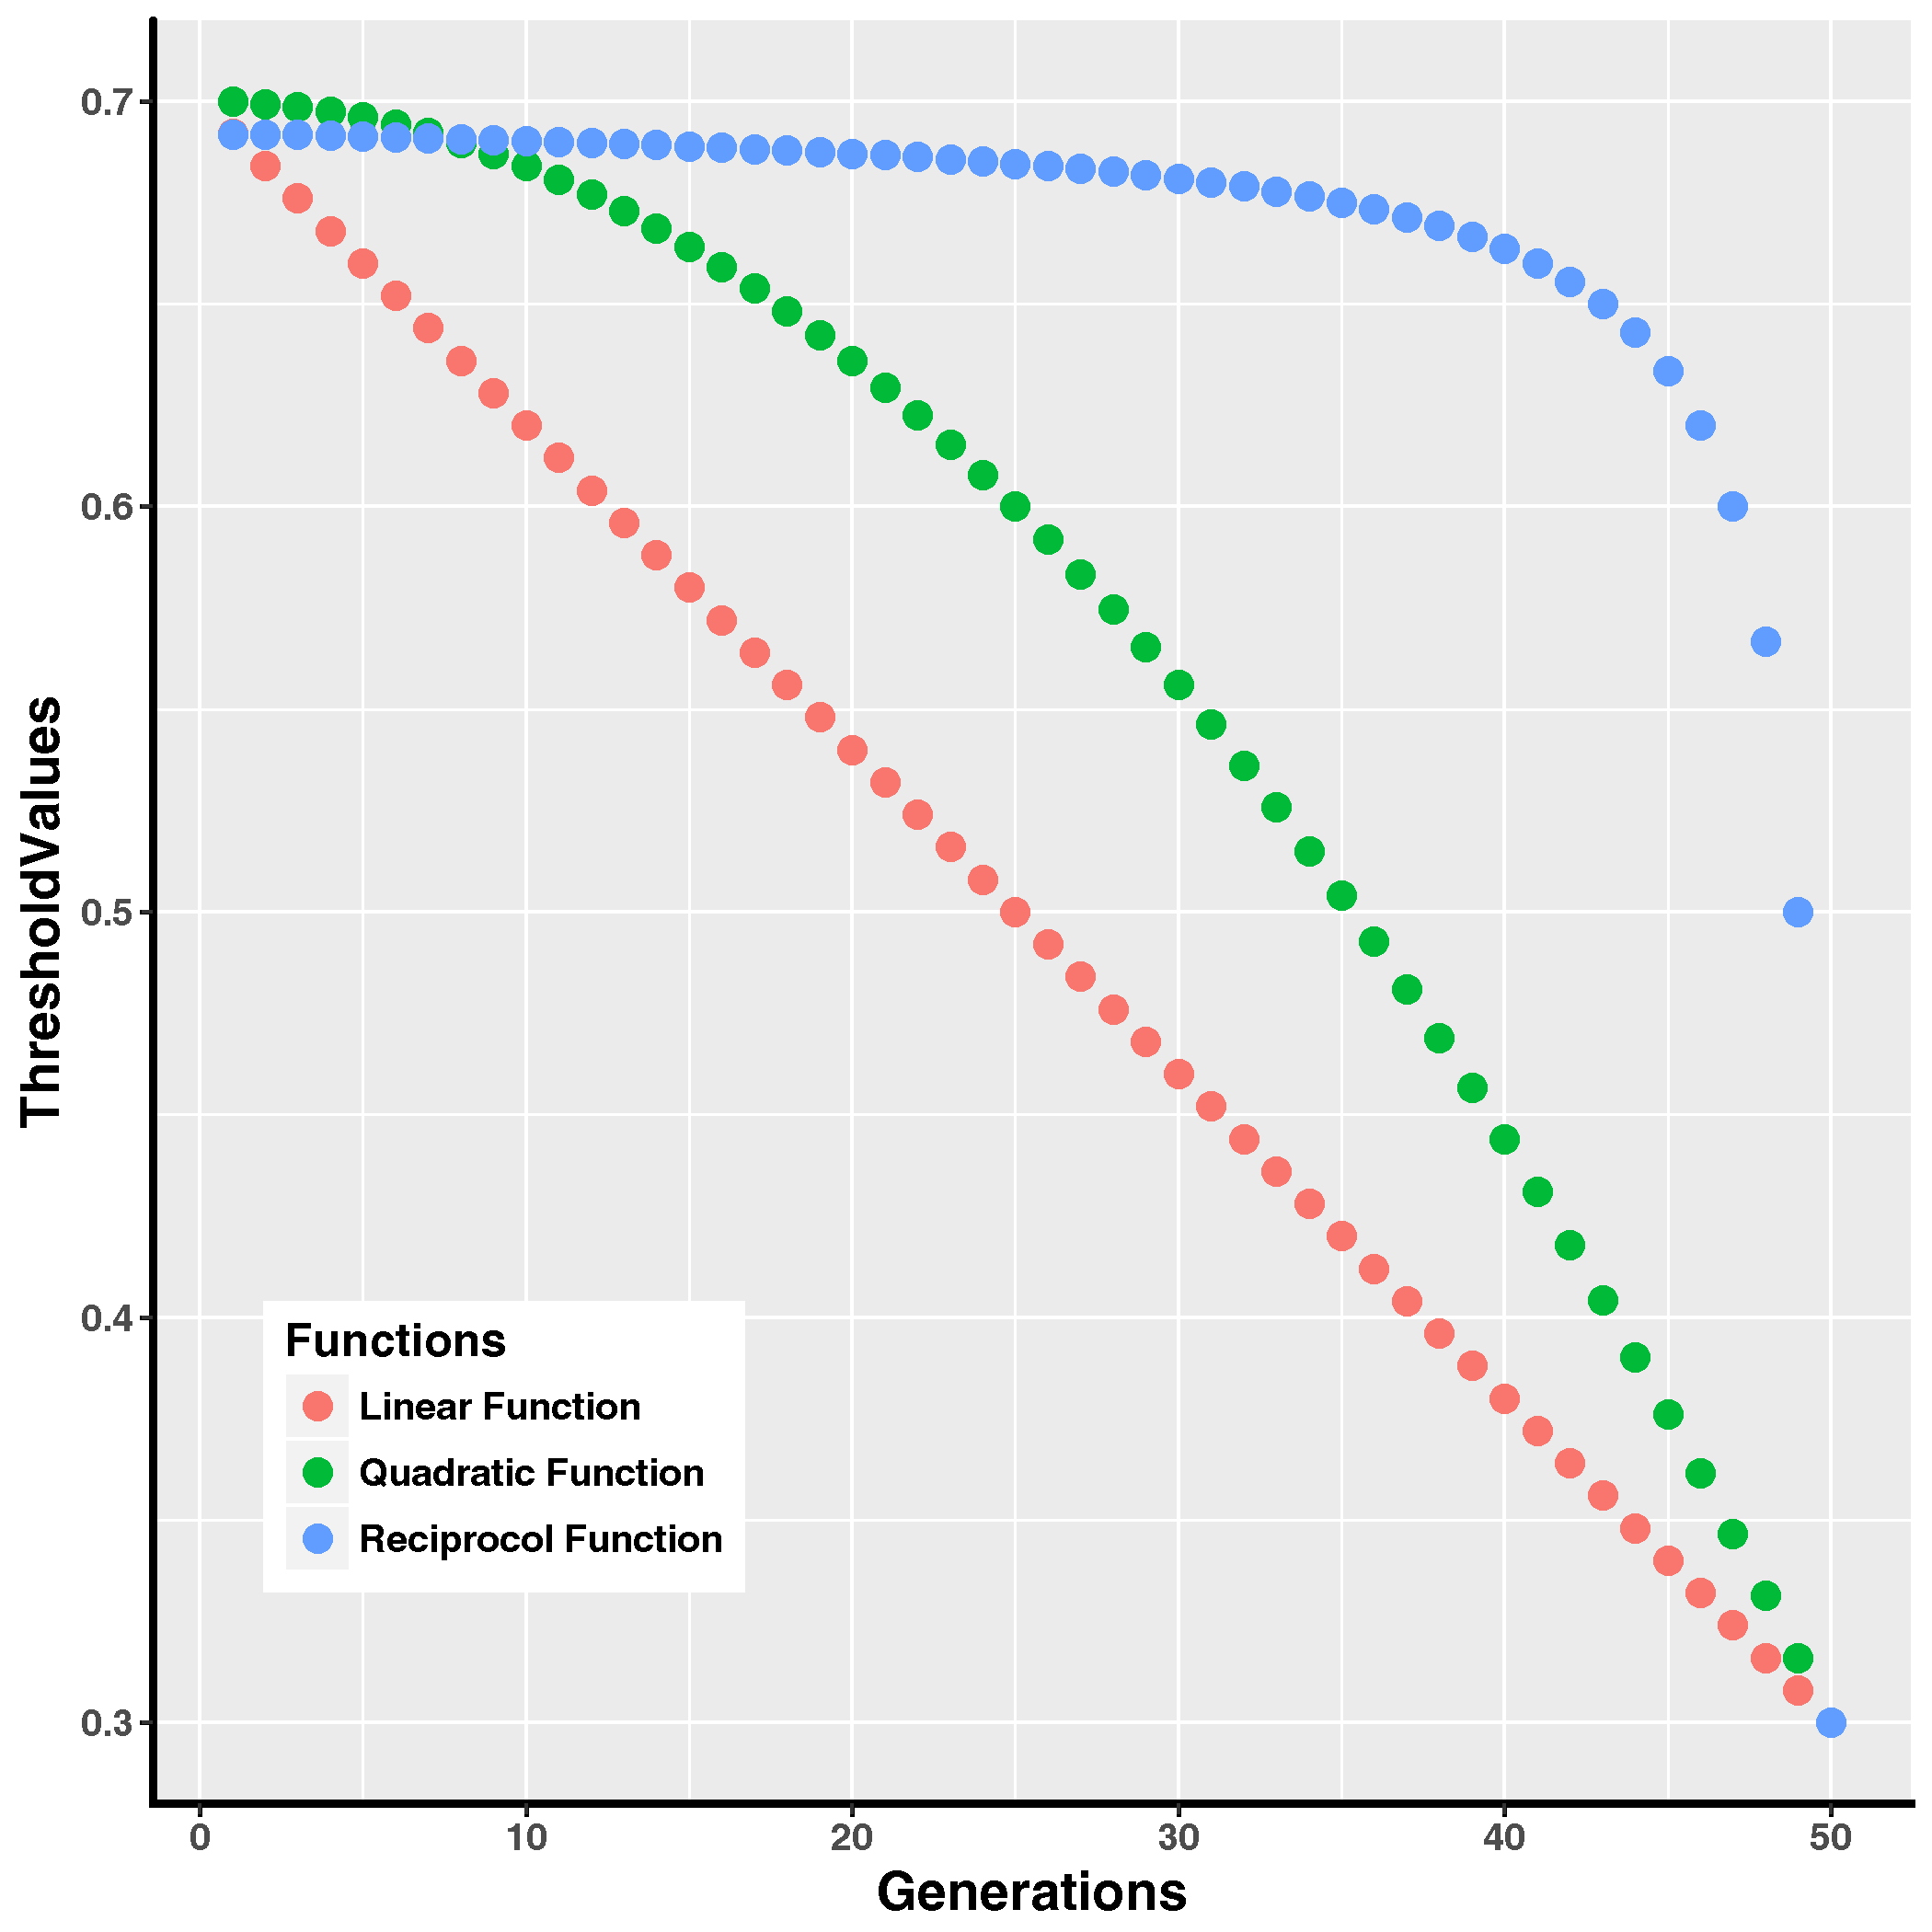
\includegraphics[width=0.3\textwidth]{pics/roundingFunctions.png}
  \caption{Trajectories of the three dynamic thresholds}
  \label{fig:dynamic}
\end{figure}
%
% The parameter $threshold$ is an empirical parameter that introduced into the algorithm.
\vspace{-3 mm}
\subsubsection{Stepped Rounding Function}
\label{sec:transfer}
% As the problem becomes getting larger and larger, the performance of evolutionary computation drops.
As the dimensionality of the problem increases, the performance of evolutionary computation drops.
It is necessary to build a system that can reuse the learned knowledge.
Transfer learning is a process to reuse the knowledge in solving unseen tasks \cite{olivas}.
This section proposes a Stepped rounding function that is embodied in the transfer learning process.

Figure \ref{fig:adaptive} shows the evolutionary process with a Stepped rounding function. % The idea of transfer learning is inspired by \cite{Verbancsics}.
Initially, the threshold $\theta$ is set to an upper bound $u$ (e.g. 0.7). Then the PSO runs with this setting for a predefined interval of $i$ (e.g. 10) generations. At the beginning of the next interval (e.g. 11) generation, the threshold $\theta$ is changed according to Equation \ref{eq:transfer} and remains until next interval. This process is repeated until the lower bound $l$ is reached. The optimization is equivalent to initializing a new set of a population with the old one. Therefore, the knowledge is inherited. An underlying assumption is that, if the particle swarm has converged within an interval, then it is better to explore a different direction. Therefore, in the next interval, the swarm will explore a slightly different area and is directed by an adjacent threshold value. 
% The potential problem of the method is that it is hard to know whether the PSO is converged. 
The Stepped rounding function is shown in Equation \ref{eq:transfer} where $\theta'$ denotes the current threshold value.

\begin{figure}[H]
 \centering
   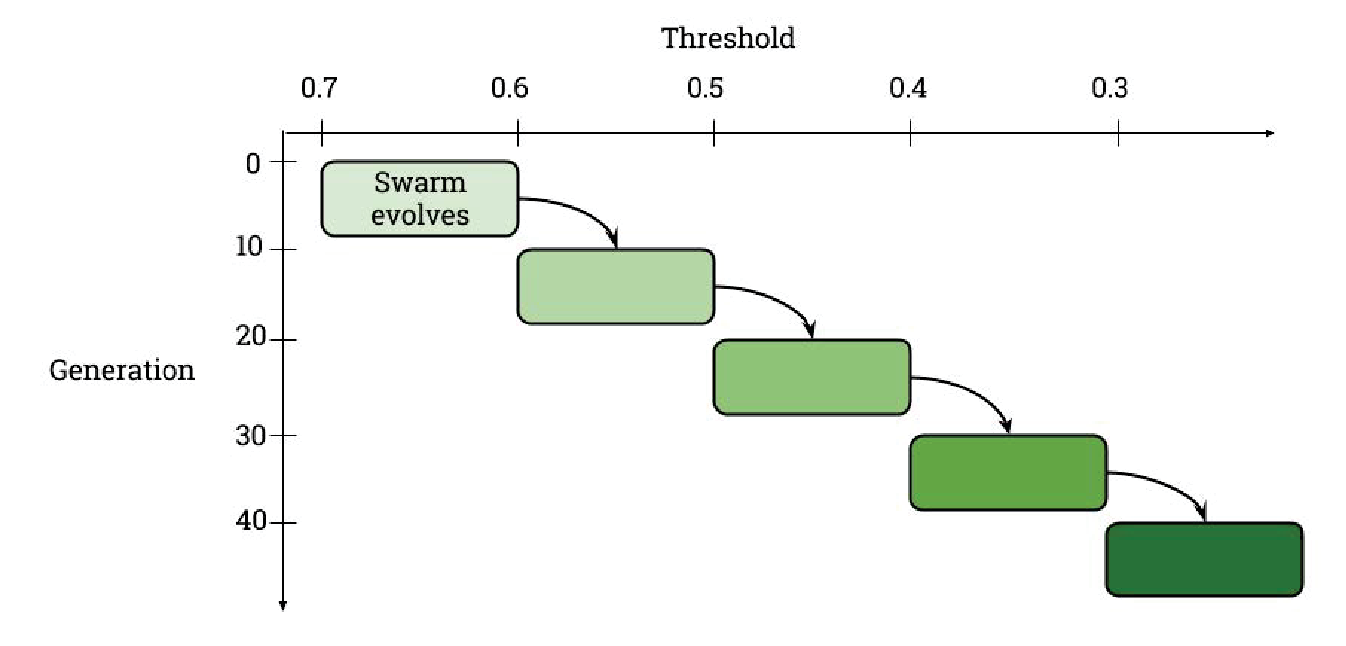
\includegraphics[width=0.4\textwidth]{pics/transfer.eps}
   \caption{Evolutionary process with the Stepped rounding function}
   \label{fig:adaptive}
 \end{figure}

\begin{small}
\begin{equation}
\label{eq:transfer}
  \theta =
  \begin{cases}
   \theta' - \frac{u - l}{(\text{max\_gen}/i - 1)} & \quad \text{if } (\text{cur\_gen}\mod i) = 0\\
   \theta' & \quad \text{otherwise} \\
  \end{cases}
\end{equation}
\end{small}

\vspace{-3 mm}
\subsection{Fitness Function and Constraint Handling}

After the particles represented as vectors have been transformed to allocation matrices, two fitness functions, Equation \ref{eq:fit-cost} and \ref{eq:fit-latency},  are used to evaluate the fitness of particles that represent allocation plans. Based on the fitness of solutions a set of non-dominated solutions are returned.

As we see in Section \ref{sec:prelimminary}, WSLAP needs to satisfy the constraint defined by Equation \ref{eq:constraint}, which means that each service needs to be allocated to at least one location. However, during the searching process of PSO, the constraint may be violated. That is, some services might be allocated to none of the locations during the process of searching.

%As in \cite{tan2016evocop}, we employ a penalty method, named \emph{death penalty}, to assign infeasible particles the highest possible fitness values. Specifically,

%\begin{equation*}
%\hat{f}_i(Y) =
%  \begin{cases}
%   \hat{f}_i(Y)  & \quad \text {if } $Y$ \text{ is feasible}\\
%   1 & \quad \text{otherwise} \\
%  \end{cases}, i = 1, 2.
%\end{equation*}

The constraint handling method used by BMOPSOCD is a ranking of violations. A solution $I$ is considered to constraint-dominate a solution $J$ if any of the following conditions is true:
\begin{enumerate}
 \item Solution $I$ is feasible while solution $J$ is not,
 \item Both solutions are infeasible and solution $I$ has fewer violations,
 \item Both solutions are feasible, and solution $I$ dominates solution $J$.
\end{enumerate}

The particle with fewer violations is always considered as a better solution. If there is only one constraint, this constraint handling method provides the same effect as the death penalty method in \cite{coello2002theoretical}.

\subsection{The BMOPSOCD algorithm for Web Service Location Allocation Problem}

Algorithm \ref{alg:BMOPSOCD} presents our BMOPSOCD algorithm for solving the WSLAP. The algorithm iteratively improves results by keeping good solutions and eliminating poor solutions.

First, a population of particles is random initialized from a uniform distribution and evaluated (lines 1--5). Notice that, instead of randomly generating population, we can design an initialization operator that only generates feasible solutions. However, this is not our focus. Therefore, this work only uses random initilization.

Next, non-dominated solutions are stored in the external archive (line 6). Lines 7--20 are the evolution process, where the population evolves maximal $MAXT$ generations and $t$ is the current generation. In each generation, solutions are ranked by their crowding distances (lines 8--9). Line 10 randomly selects a global best since they are equally good. Lines 12--13 update position and velocity values. Line 14 guarantees a particle will not leave its domain by reversing its direction. Lines 15 conducts the mutation, where $P_m$ is the mutation rate (see Section. \ref{sec:parameters}). Line 16--17 round the population and evaluate them with fitness functions. Line 19 updates the best solutions in the archive.

The selection of $pbest$ and $gbest$ is one of the key steps in BMOPSOCD. $pbest$ is the personal best solution of each particle in a population. The $pbest$ is updated only if the new particle dominates the current one. Otherwise, it remains unchanged. In the BMOPSOCD, any non-dominated solutions in the archive can be a $gbest$. Therefore, it is important to ensure that the particles move to an unexplored area. The $gbest$ is selected from non-dominated solutions with the highest crowding distance value. It ensures that the swarm move to a less crowded area.


\begin{algorithm}[!htb]
 \caption{BMOPSOCD for WSLAP}
 \footnotesize
 \textbf{Inputs:} \\
  Cost Matrix $C$, \\
  Server network latency matrix $L$, \\
  Service invocation frequency matrix $F$ \\
 \textbf{Outputs:}
  Pareto Front: the $Archive$ set

 \begin{algorithmic}[1]
  \State Initialize each individual $X_{ij}$ in a Population $P$ with a random real value $\in$ (0, 1).
  \State Initialize $v_i$ = 0
  \State \textbf{For each individual $i$ in $P$ Rounding and Evaluating fitness}
  \State Initialize $pbest$ of each individual $i$.
  \State Initialize $gbest$
  \State Initialize $Archive$ with non-dominated vectors in $P$

  \Repeat
   \State Compute the crowding distances of each solution $i$ in $Archive$
   \State Sort solutions in $Archive$ in descending crowding distances
   \For ( each particle)
    \State Randomly select the global best guide for $P[i]$ from a specified top portion of the sorted archive $A$ and store its position to $gbest$.
    \State Compute the new velocity $v_i$ using Eq.\ref{eq:updateVelocity}
    \State Update its position $x_i$ using Eq.\ref{eq:updatePosition}
    \State If $X_{ij} >$ 1 or $X_{ij} <$ 0, set its value to 1 or 0 and multiply its velocity by -1.
    \State If ($t < (MAXT * P_m)$), apply Mutation
    \State \textbf{Rounding and Evaluating fitness}
    \State Update its $pbest$
    \EndFor
  \State Insert new non-dominated solutions into $Archive$, remove dominated solutions from $Archive$
  \State $t$ increment by 1
  \Until{ $t$ reaches $MAXT$}
  \State return $Archive$
 \end{algorithmic}
 \label{alg:BMOPSOCD}
\end{algorithm}

The fitness of particles can be evaluated using the objective functions presented in Equation  \ref{eq:fit-cost} and \ref{eq:fit-latency}. Line 12 updates velocity $v_i$ as:
\begin{small}
\begin{equation}
 v_{id} = w * v_{id} + c_1 * r_{1i} * (p_{id} - x_{id}) + c_2 * r_{2i} * (p_{pg} - x_{id})
\end{equation}
\end{small}
\noindent where $w$ is the inertia weight, $c_1$ and $c_2$ are the acceleration factors, $r_{1i}$ and $r_{2i}$ are the random variables sampled from the uniform distribution between 0 and 1, $v_{id}, x_{id}, p_{id}$ and $g_{d}$ denote the value in dimension $d$ of $\vec{v_i}, \vec{x_i},\vec{p_i}$ and $\vec{g}$, respectively.  Note that the main difference between our algorithm and the original \cite{Raquel} are in Lines 3 and 16, which is the use of rounding function. For WSLAP, the decision variable is binary. Therefore, in our algorithm (Line 3 and 16) we apply a rounding function to transform continuous values to binary values.

The mutation operator (Line 15) changes the value of each dimension of an individual according to a nonlinear function \cite{1304847}. The nonlinear function is related to the total number of iteration and the current number of iteration. The mutation operator is designed to increase the diversity of the initial population.

% was introduced by Carlos Coello \cite{1304847} to improve the exploration capability at the beginning of the search. At the beginning, the mutation operator affects the entire population. As the iteration increases, the mutation operator affects less population . The intuition of the mutation operator is to prevent the PSO from stucking at local optima at the early stage. Meanwhile, mutation affects less population at the late stage to encourage the convergence of PSO.

In Line 19, dominated solutions from the \textit{archive} are removed. For example, if there are two solutions $A$ with cost of 560 and overall latency as 1120.5 and $B$ with cost of 780 and overall latency as 1589.9 in the archive. In this case, solution $A$ dominates $B$ since $A$'s cost and latency are better than $B$'s. Then solution $B$ is removed
from the \textit{archive}. At the end of the algorithm, an \textit{archive} with non-dominated
solutions is returned as the best solutions found during the entire evolutionary process.

%\section{Experiment Design}
\section{Experiment Design} \label{sec:experiment}
\label{sec:exp}

This study proposes a multi-objective approach to WSLAP to produce well-distributed Pareto-optimal solutions. Meanwhile, the performance of the proposed algorithm performs well with the increasing size of problems. 
The above section presents our BMOPSOCD approach to WSLAP. We develop static and dynamic rounding methods with different threshold settings. We conduct a set of experiments over three variant of the proposed algorithm. The first variant uses the static threshold. We study the influence of different threshold values; the second variant uses the dynamic rounding functions. We examine the effect of three dynamic rounding functions; The third variant is the Stepped rounding function. We compare its results with dynamic functions. In addition, we make a comparison between a dynamic function with a congregation of
several static rounding functions with different thresholds. 
Lastly, we conduct an experiment considering the overall performance of a BMOPSOCD with a dynamic rounding function in comparison with three other algorithms: PSO, BNSPSO and NSGA-II (see \cite{Tan2016}). 

All algorithms were implemented in R version 3.3.3 and the experiments were conducted on an i7-4790 3.6 GHz with 8GB of RAM memory running Linux Arch 4.9.6.
\subsection{Comparison Design}
We use different ways to compare three variants of BMOPSOCD, and BMOPSOCD with other algorithms (e.g NSGA-II). The major difference is that we compare three variants with the solutions from a single run while we compare BMOPSOCD and other algorithms with their best solutions from 40 runs.

Explicitly, for comparing three variants of BMOPSOCD, we first find out the median HyperVolume value (explained in Section \ref{sec:metrics}) in 40 runs. Then we find out in which run that the variant of BMOPSOCD produces the median HyperVolume value. Finally, we plot the solutions from that run in terms of two objectives fitness values.

To compare with BMOPSOCD, we first aggregate the solutions from 40 runs and then apply an non-dominated sorting on the aggregated results to find the best results from that algorithm. Finally, we plot the solutions. 

All fitness values are normalized between 0 and 1 with a linear normalization method described in \cite{Tan2016}. 
The normalization method requires the maximum and minimum values of cost and response time 
that we found during optimization. 

We obtained these extreme values as follows. For each instance, we collected the solutions from all the four compared algorithms: NSGA-II, BPSO, NSPSO, and BMOPSOCD. Then, we applied non-dominated sorting on these solutions to obtain the non-dominated solutions. Finally, we can find the extreme values of cost and response time from the non-dominated solutions abtained from all the solutions found by all the compared algorithms.

\subsection{Test instances}
\label{sec:datasets}


% The test instances are combined with a real-world dataset \textit{WS-Dream} \cite{Service_dataset} and synthetic datasets \cite{Tan2016a}. 



We designed 14 test instances with increasing size of search space (see Table \ref{test_instances}). The instances were generated randomly, and thus were not biased to any algorithm. The search space is decided by the number of services and candidate locations (e.g $2^{service \cdot candidate}$). Because the computation complexity is not solely determined by the search space of test instances, from instance 3 onwards, for each search space, we vary the number of user centers. 



We constructed test instances based on real-world WS-Dream dataset \cite{Service_dataset}. The dataset
contains only the latencies between candidate locations and user centers, but lacks the deployment costs for candidate locations and invocation frequencies for web services. Therefore, to generate a complete WSLAP instance, we randomly generated the deployment costs for candidate locations according to a normal distribution with the mean of 100 and standard deviation of 20. We generated the invocation frequencies from a uniform distribution between 1 and 120. 

% The \textit{WS-Dream} dataset includes a network latency matrix between 339 user centers and 5825 candidate locations. In this project, there are mainly three matrices to be provided: network latencies between candidate locations and user centers, deployment cost in candidate locations, and web service invocation frequency. In principle, deployment cost can be either fixed fees (monthly rent) or variable fees (e.g. depending on storage and other resource usages). For the sake of simplicity, we consider fixed deployment fee.

% Table \ref{tab:problem} shows fourteen representative instances, listed with increasing size.

\begin{table}[h]
\footnotesize
\centering
\scalebox{0.8}{
\begin{tabular}{l|c|c|c|c}
\hline
Test instances   & \multicolumn{1}{l|}{\begin{tabular}[c]{@{}l@{}}No. of \\ Services\end{tabular}} & \multicolumn{1}{l|}{\begin{tabular}[c]{@{}l@{}}No. of \\ Candidate Locations\end{tabular}} & \multicolumn{1}{l|}{\begin{tabular}[c]{@{}l@{}}No. of \\ user centers\end{tabular}} & \multicolumn{1}{l}{\begin{tabular}[c]{@{}l@{}}Size of \\ search space\end{tabular}}\\ \hline
instance 1  & 20                                                                             & 5                                                                                         & 10 & $2^{100}$ \Tstrut                                                                                 \\ \hline
instance 2  & 20                                                                                                                                                                    & 10 & 10 & $2^{200}$ \Tstrut                                                                                \\ \hline
instance 3  & 50                                                                             & 15                                                                                        & 20 & $2^{750}$ \Tstrut                                                                                 \\ \hline
instance 4  & 50                                                                             & 15                                                                                        & 40& $2^{750}$  \Tstrut                                                                                \\ \hline
instance 5  & 50                                                                             & 25                                                                                        & 20 & $2^{1250}$ \Tstrut                                                                                 \\ \hline
instance 6  & 50                                                                             & 25                                                                                        & 40 & $2^{1250}$ \Tstrut                                                                                  \\ \hline
instance 7  & 100                                                                            & 15                                                                                        & 20 & $2^{1500}$  \Tstrut                                                                                \\ \hline
instance 8  & 100                                                                            & 15                                                                                        & 40& $2^{1500}$  \Tstrut                                                                                \\ \hline
instance 9  & 100                                                                            & 25                                                                                        & 20 & $2^{2500}$ \Tstrut                                                                                 \\ \hline
instance 10 & 100                                                                            & 25                                                                                        & 40 & $2^{2500}$  \Tstrut                                                                                \\ \hline
instance 11 & 200                                                                            & 25                                                                                        & 40 & $2^{5000}$  \Tstrut                                                                                \\ \hline
instance 12 & 200                                                                            & 25                                                                                        & 80& $2^{5000}$    \Tstrut                                                                              \\ \hline
instance 13 & 200                                                                            & 40                                                                                        & 40& $2^{8000}$   \Tstrut                                                                               \\ \hline
instance 14 & 200                                                                            & 40                                                                                        & 80 & $2^{8000}$  \Tstrut                                                                                \\ \hline
\end{tabular}
}
\caption{Test instances}\label{test_instances}
\end{table}



\subsection{Performance Metrics}
\label{sec:metrics}
We use HyperVolume (HV) and IGD as the evaluation metrics. HyperVolume indicator \cite{Zitzler1998, 7360024} is a measure used in evolutionary multi-objective optimization, which reflects the volume enclosed by a solution set and a reference point. A larger HyperVolume value indicates a better solution set. The IGD \cite{1501598} is a modified version of generational distance \cite{veldhuizen99} as a way of estimating how far the elements in the true Pareto front are from those in the non-dominated set produced by an algorithm. IGD calculates the sum of the distances from each point from the true Pareto front to the nearest point from the non-dominated set produced by an algorithm. The lower the IGD, the better quality the solution is. Calculating the IGD value needs a true Pareto front. For our problem, the true Pareto front is unknown. Therefore, an approximated Pareto front is produced by combining all the solutions produced by the four compared algorithms (BMOPSOCD, NSGA-II, BNSPSO, BPSO) and then applying a non-dominated sorting to obtain the final non-dominated set. The approximated Pareto front dominates all the other solutions we found.



\subsection{Parameter Settings}
\label{sec:parameters}
The parameters of the PSO algorithms are set as follows. We applied static inertia weight and set $w$ to 0.4. Although it is found in \cite{xin2009particle} that inertia weight $w$ decreasing from 0.9 to 0.4 provides excellent results, this work only focuses on rounding functions. Therefore, the influence of dynamic $w$ has to be eliminated. Mutation probability is in range of [0, 1]. This study follows the original paper's \cite{Raquel} and set $P_m$ to 0.5. The cognitive parameter and social parameter $c_1$ and $c_2$ are generally selected from the range of [0, 4]. This study sets both parameters to 1 \cite{Raquel} so that cognitive and social parameter have an equal influence on the swarm. The archive size and a population size are set to 250 and 50 respectively according to the original paper's \cite{Raquel} recommendation. Generally, the population size has a relation with the search space. A larger population size denotes a stronger search ability because 
more space are explored \cite{qi1994theoretical}.
Our study focuses on the binary PSO technique instead of selecting the best parameter set. Therefore an empirical value is selected and the maximal number of iteration is set to 50 in all experiments. 
The ``empirical value'' means we tried several values for the number of generation and see whether the solutions has converged (has little changes of fitness values between two consecutive generations). 
We chose the minimum number of generation that allows all the four compared algorithms converging. Hence, it is fair for all compared algorithms


We used (1, 1) as the reference point in HyperVolume. Because we normalize two objectives between 0 and 1, reference point (1, 1) is the extreme point of objective values. Moreover, we do not have particular preference to objectives. Therefore, a balanced point (1, 1) is suitable for the reference point.

For each experiment, the proposed algorithm was run for 40 times independently. The best results of all the runs are compared.  To obtain the \emph{best result} of 40 runs, the results of all 40 runs are combined and sorted by the fast non-dominated sorting \cite{nsgaii}.

% Please add the following required packages to your document preamble:
% \usepackage{booktabs}
% Please add the following required packages to your document preamble:
% \usepackage{booktabs}
\begin{table}[]
\centering
\scalebox{0.8}{
\begin{tabular}{@{}cccc@{}}
\toprule
Parameter & value & Parameter          & value  \\ \midrule
$w$         & 0.4 \cite{xin2009particle}   & population size    & 250 \cite{Raquel}    \\
$P_m$      & 0.5  \cite{Raquel} & archive size       & 250 \cite{Raquel}    \\
$c_1$      & 1 \cite{Raquel}    & iteration          & 50 \cite{Raquel}     \\
$c_2$      & 1 \cite{Raquel}    & HV reference point & (1, 1) \cite{Raquel} \\ \bottomrule
\end{tabular}}
\caption{Parameter Settings for BMOPSOCD}
\label{parameter}
\end{table}


% Please add the following required packages to your document preamble:
% \usepackage{booktabs}

\subsection{Experiments on Rounding Functions}\label{sec:expRound}
This section designs four experiments to study the effect of different types of rounding functions. We applied Wilcoxon signed rank test on all results between variants of BMOPSOCD. We chose these four representative instances (instances 2 to 5) to show the results. The other test instances showed similar patterns.

% The cost constraint is not considered in these experiments since it is not the study priority.
% The repair function of NSGA-II will also only use the Web service number constraint.

\subsubsection{Static Rounding Function}
\label{sec:static_exp}
There are two questions that we would like to answer with this experiment. The first question is \textit{what the influence of the threshold is}. The second question is \textit{how to select a proper static threshold}. We conduct several experiments to evaluate the performance of various threshold values ranging from 0 to 1 divided equally into 10 segments. 

\subsubsection{Result Analysis of Static Rounding Function}
\label{sec:result_static}
\begin{figure}[h!]
	\centering
	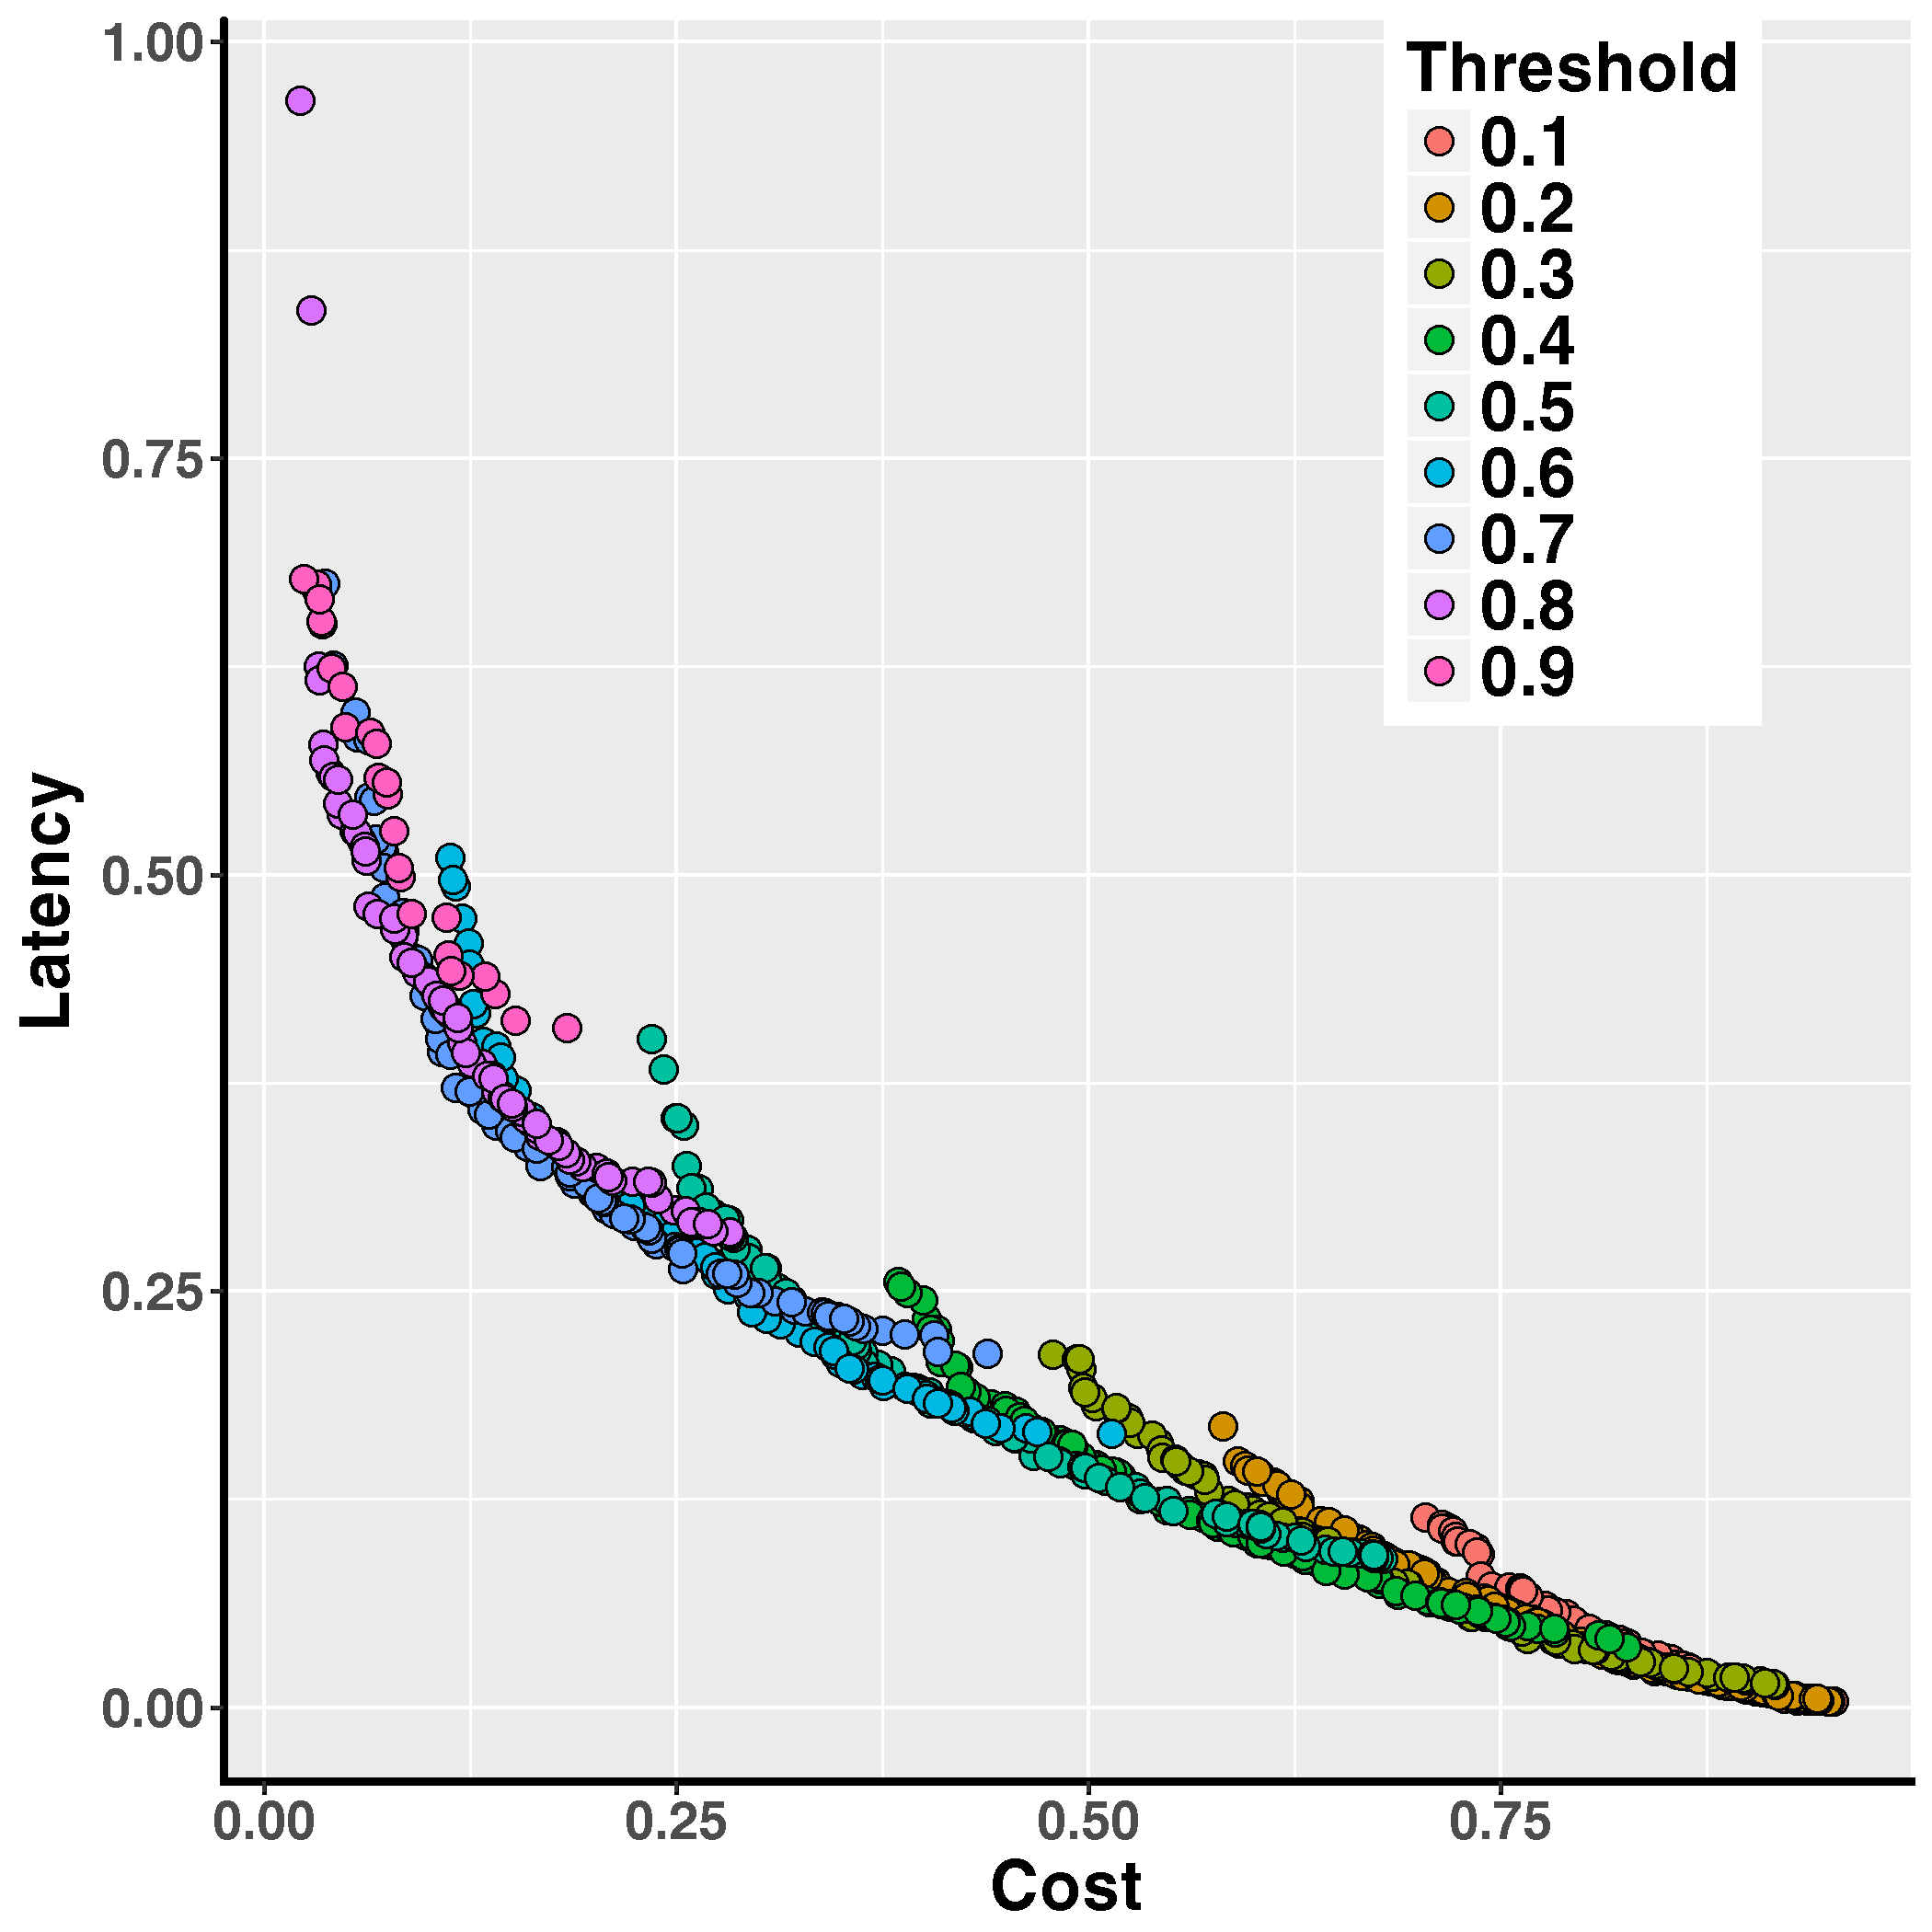
\includegraphics[width=0.3\textwidth]{pics/static_threshold_problem_extra2.png}
	\caption{Solve Test instance 2 with Static thresholds ranging from 0.1 to 0.9}
	\label{fig:fullThreshold}
\end{figure}

A representative result is given in Figure \ref{fig:fullThreshold}, where each color represents a threshold value and each point denotes a service allocation solution in the 2D objective space. It shows that in the BMOPSOCD with a different static threshold value will lead to solutions covering a different partial region of the Pareto front. 

The impact of a static threshold can be explained as a preference factor between two objectives. Take the threshold value of 0.7 as an example, 
when the rounding function rounds a real value to a binary value with the threshold of 0.7, it means that 70\% of probability rounds this value to zero. It denotes that there are 70\% of chances not deploying a web service in a location. 
Intuitively, the optimization with threshold of 0.7 would consider optimizing cost over latency by deploying fewer web services. The swarm is under the 
guidance of a ``savings'' policy. 



% This effect can be observed in Figure \ref{fig:staticFunctions} where all four test the solutions with 0.7 threshold scattered along the area with lower cost and higher latency (e.g. orange points). On the other hand, the solutions with $\theta < 0.5$favor quality
% over cost, that is, more web services are deployed. 

Another important point is that, the solutions generated using various thresholds, from 0.3 to 0.7, almost cover the entire Pareto front (with the zero cost-fitness eliminated because of the service number constraint). That is, the solutions from thresholds under 0.3 and greater than 0.7 have trivial improvement for a final solution set \ref{fig:staticFunctions}.
Therefore, 0.3 and 0.7 can be set as the lower and upper bound of a variant threshold without losing many solutions.

The experimental results answered the first question: \textit{the influence of different thresholds}. 
However, it does not offer a guideline for selection of a proper threshold, because none of the solutions could cover the entire Pareto front.
The combination of all the results boosts the diversity of the non-dominated set. However, repeating the experiment with different threshold values is time consuming. It is necessary to discover a method with widely spread solutions as well as a low computational complexity.
The observation of thresholds inspires the development of the dynamic rounding functions.

\begin{figure}[h!]
   \centering
   \begin{subfigure}{0.49\linewidth}
       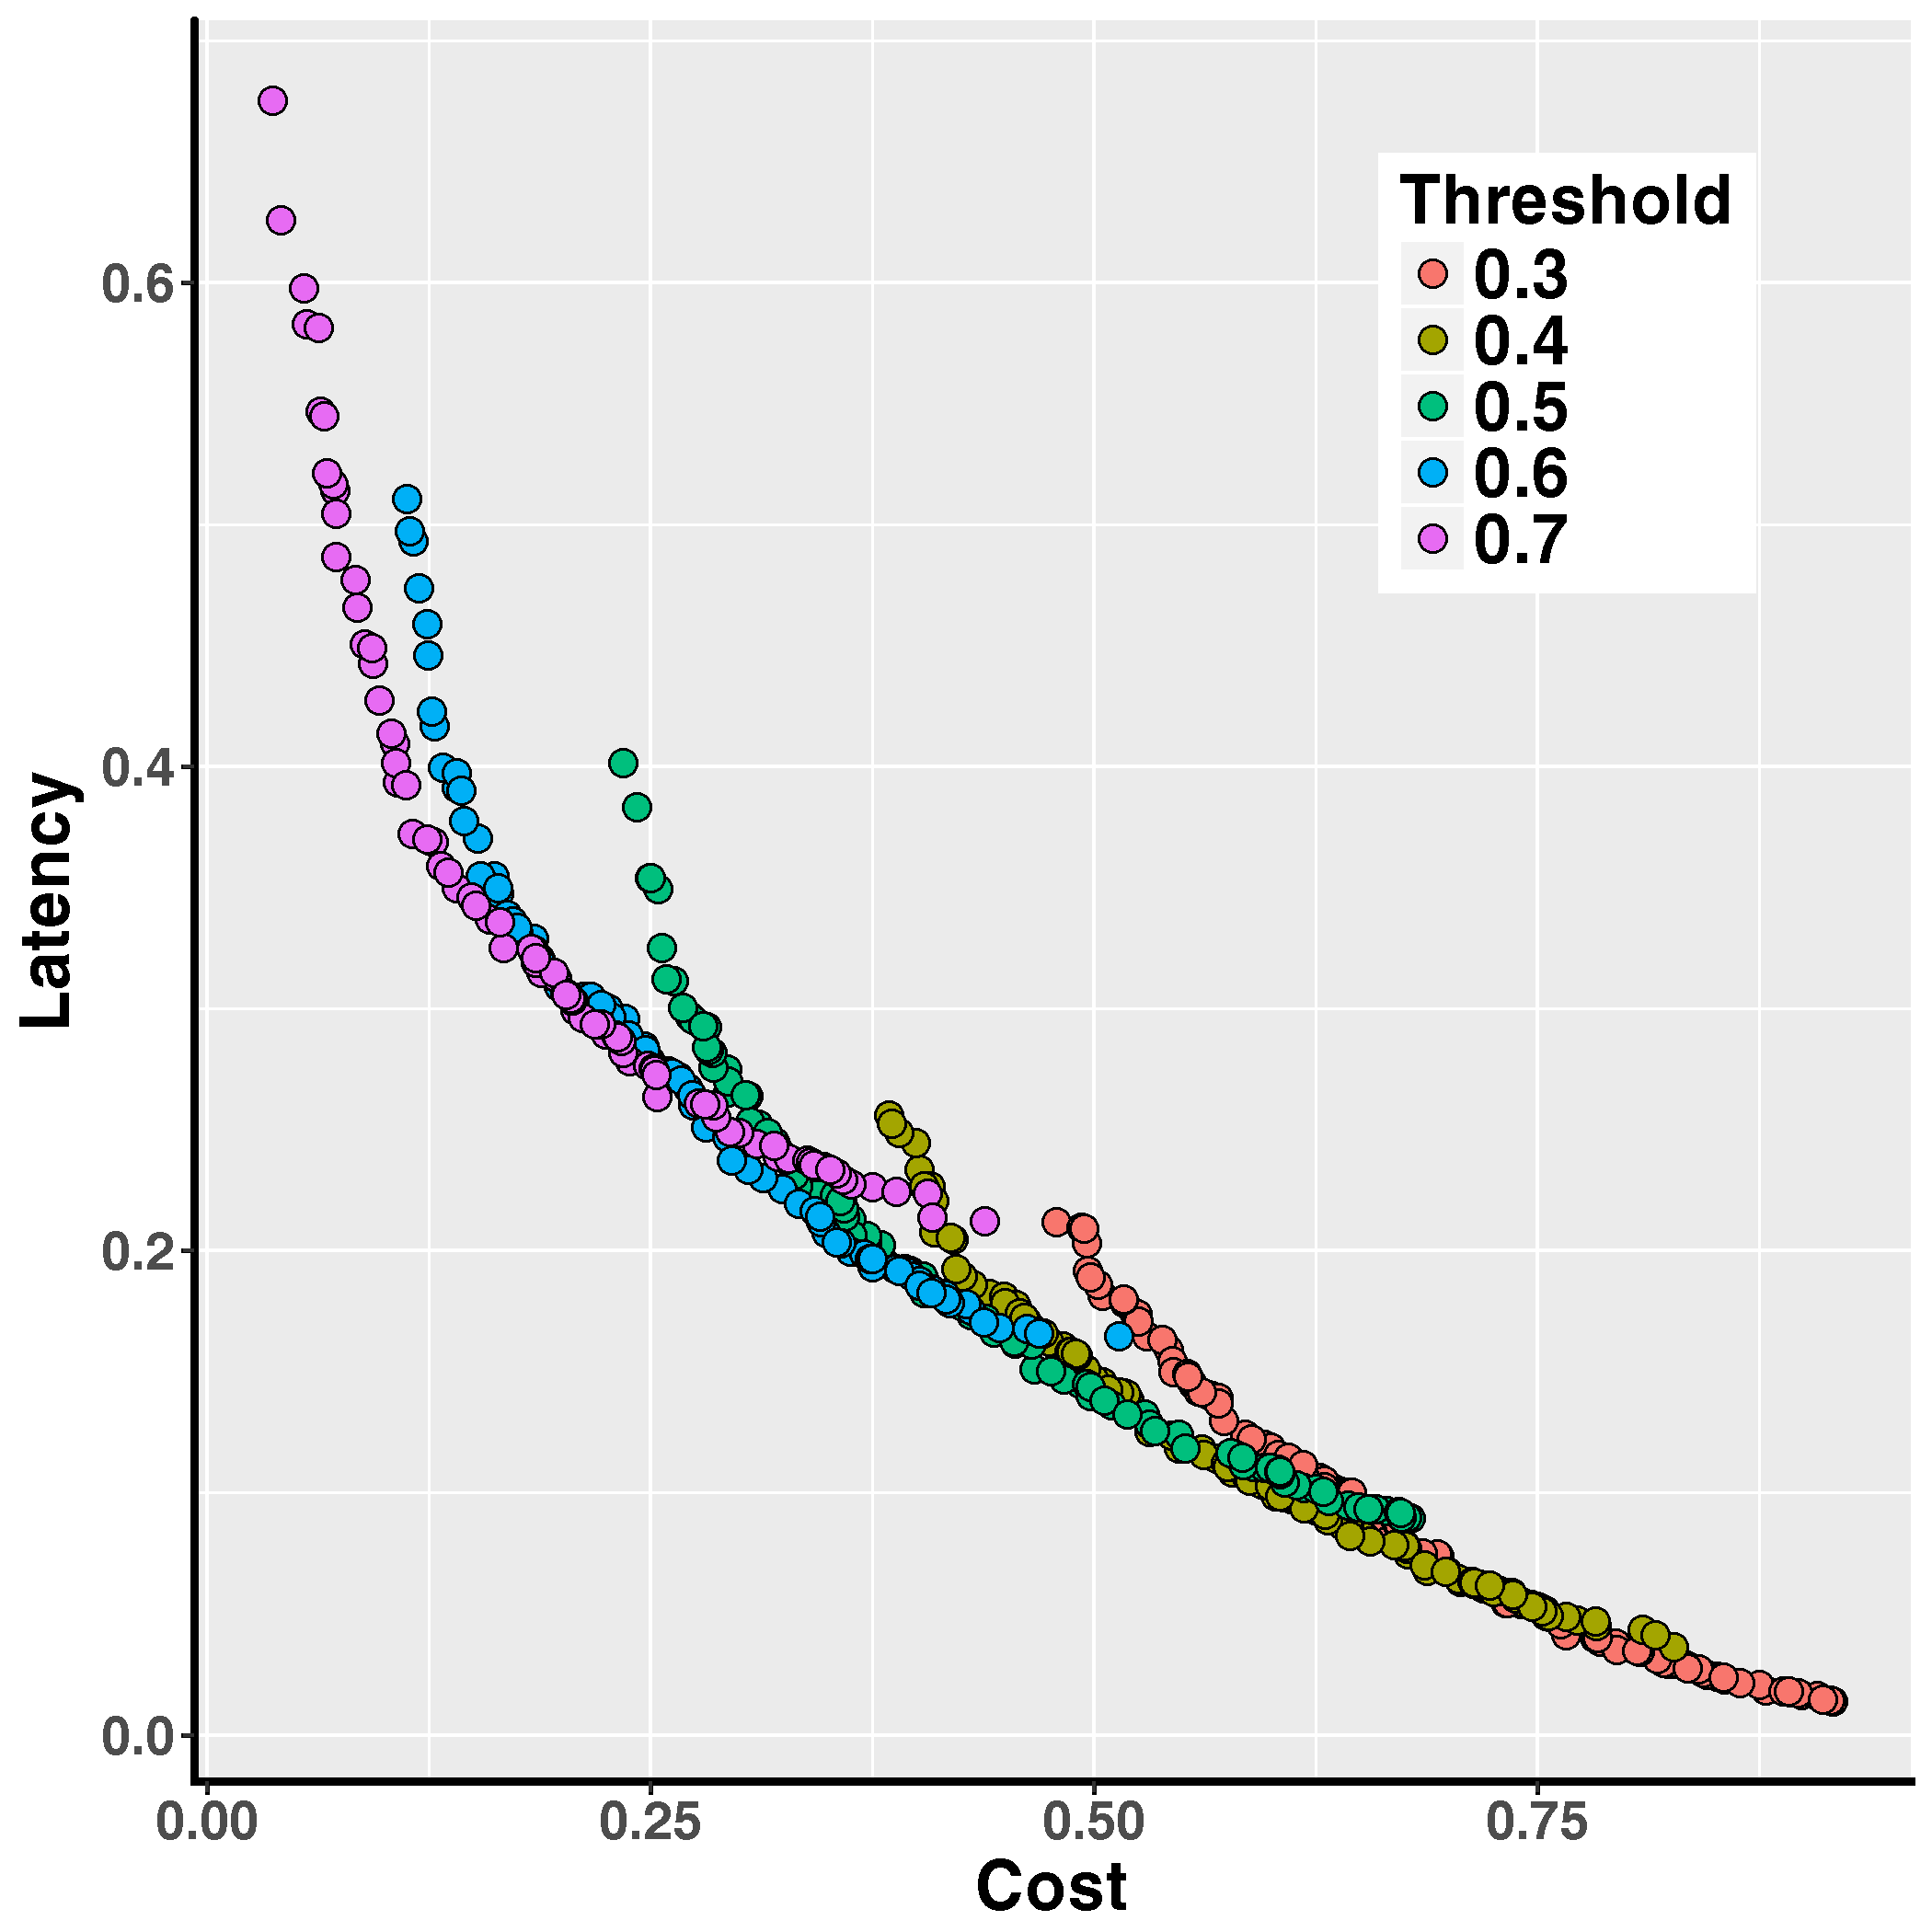
\includegraphics[width=\textwidth]{pics/static_threshold_problem_2.png}
    \caption{instance 2}
   \end{subfigure}
   \begin{subfigure}{0.49\linewidth}
       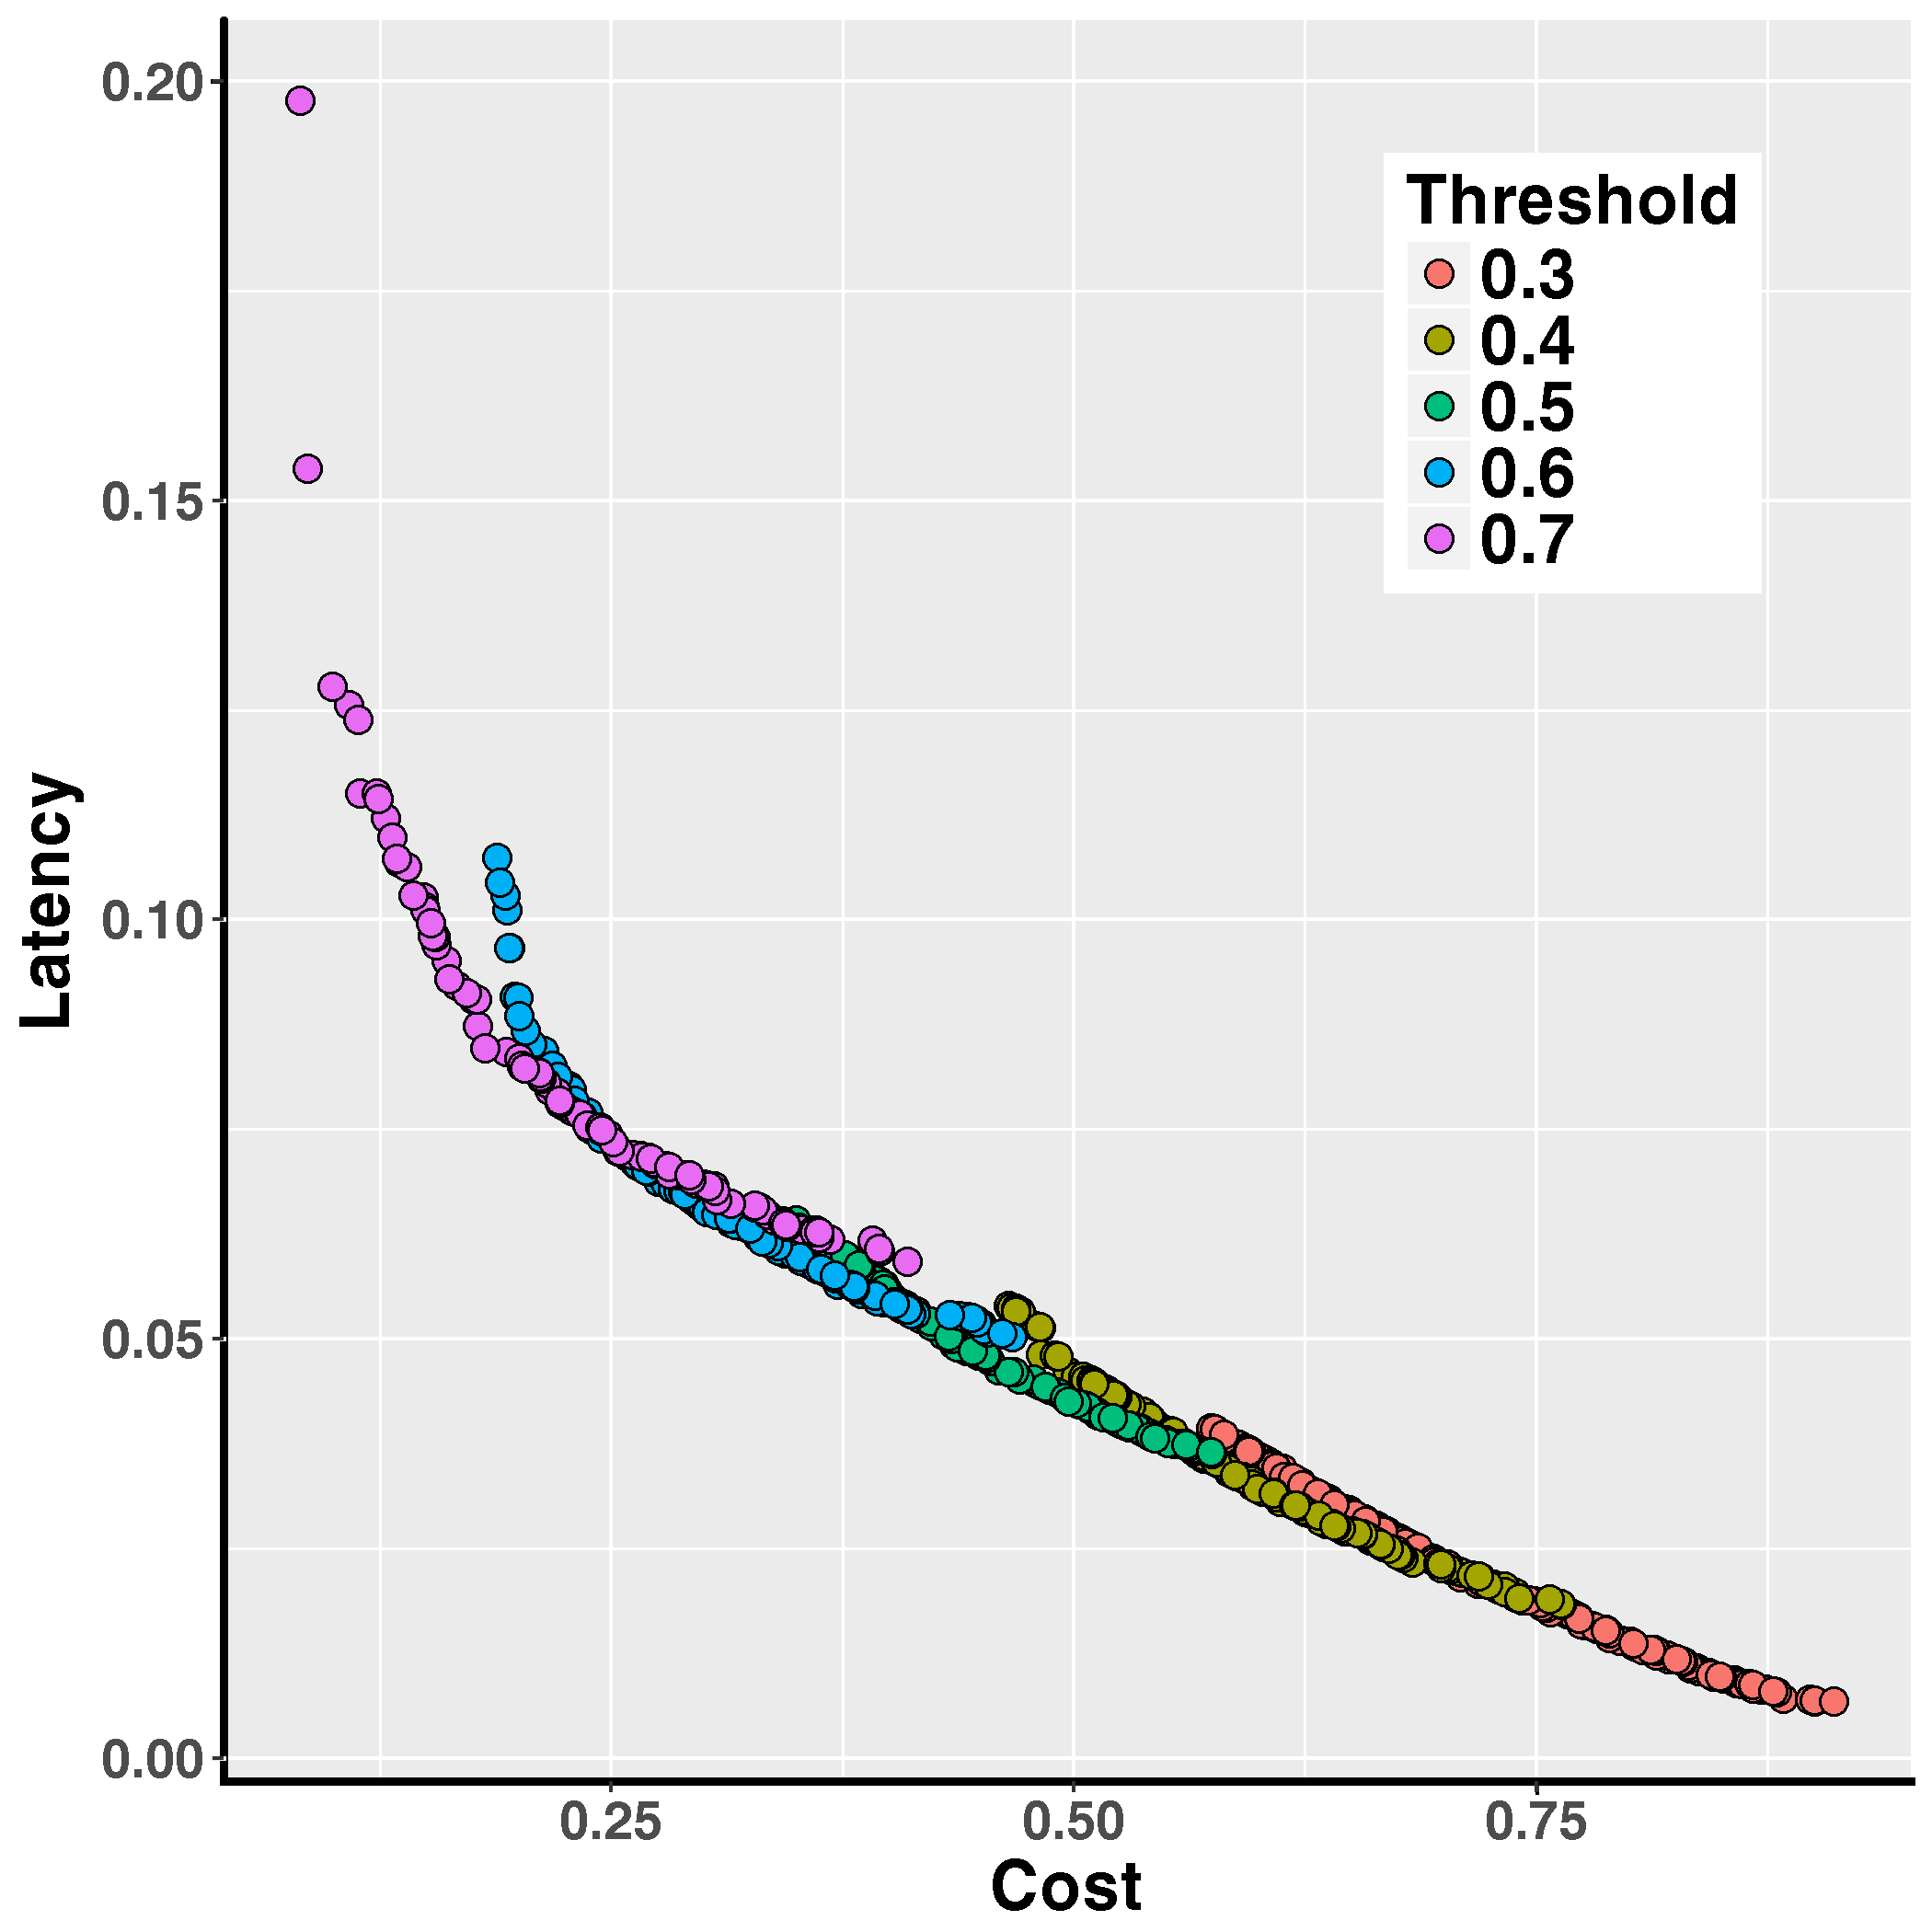
\includegraphics[width=\textwidth]{pics/static_threshold_problem_3.png}
    \caption{instance 3}
   \end{subfigure}
   \begin{subfigure}{0.49\linewidth}
       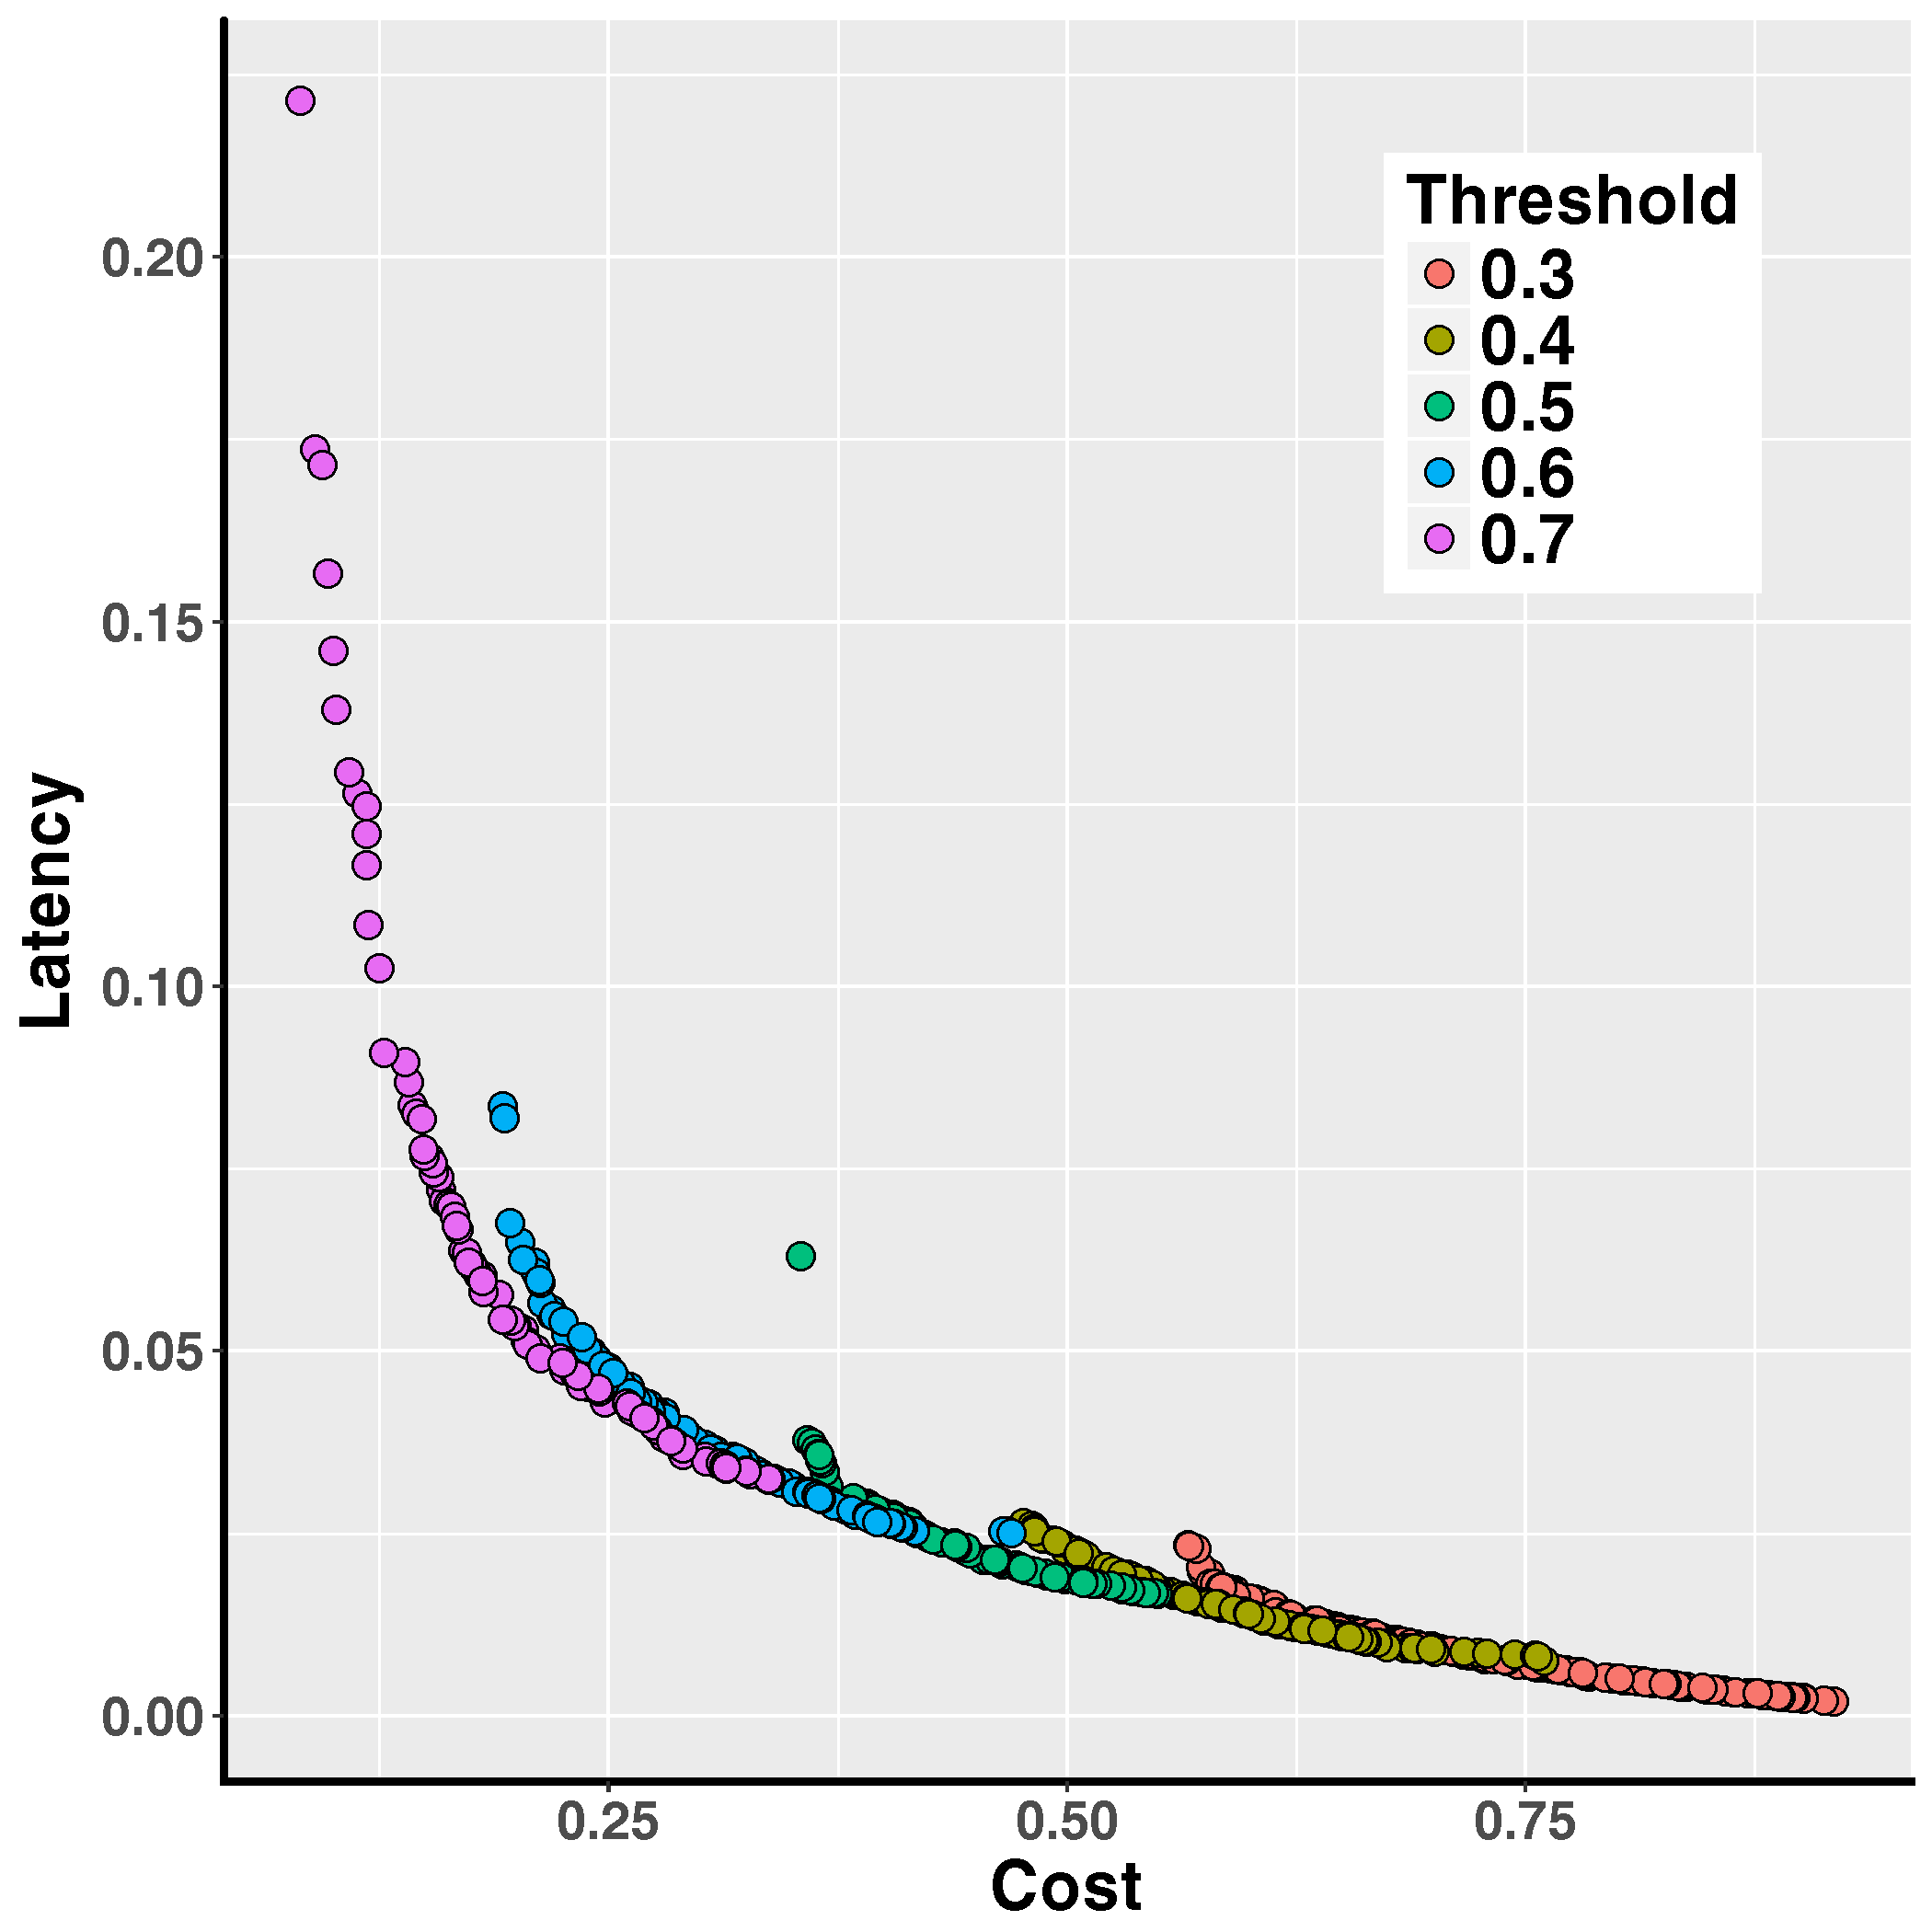
\includegraphics[width=\textwidth]{pics/static_threshold_problem_4.png}
    \caption{instance 4}
   \end{subfigure}
   \begin{subfigure}{0.49\linewidth}
       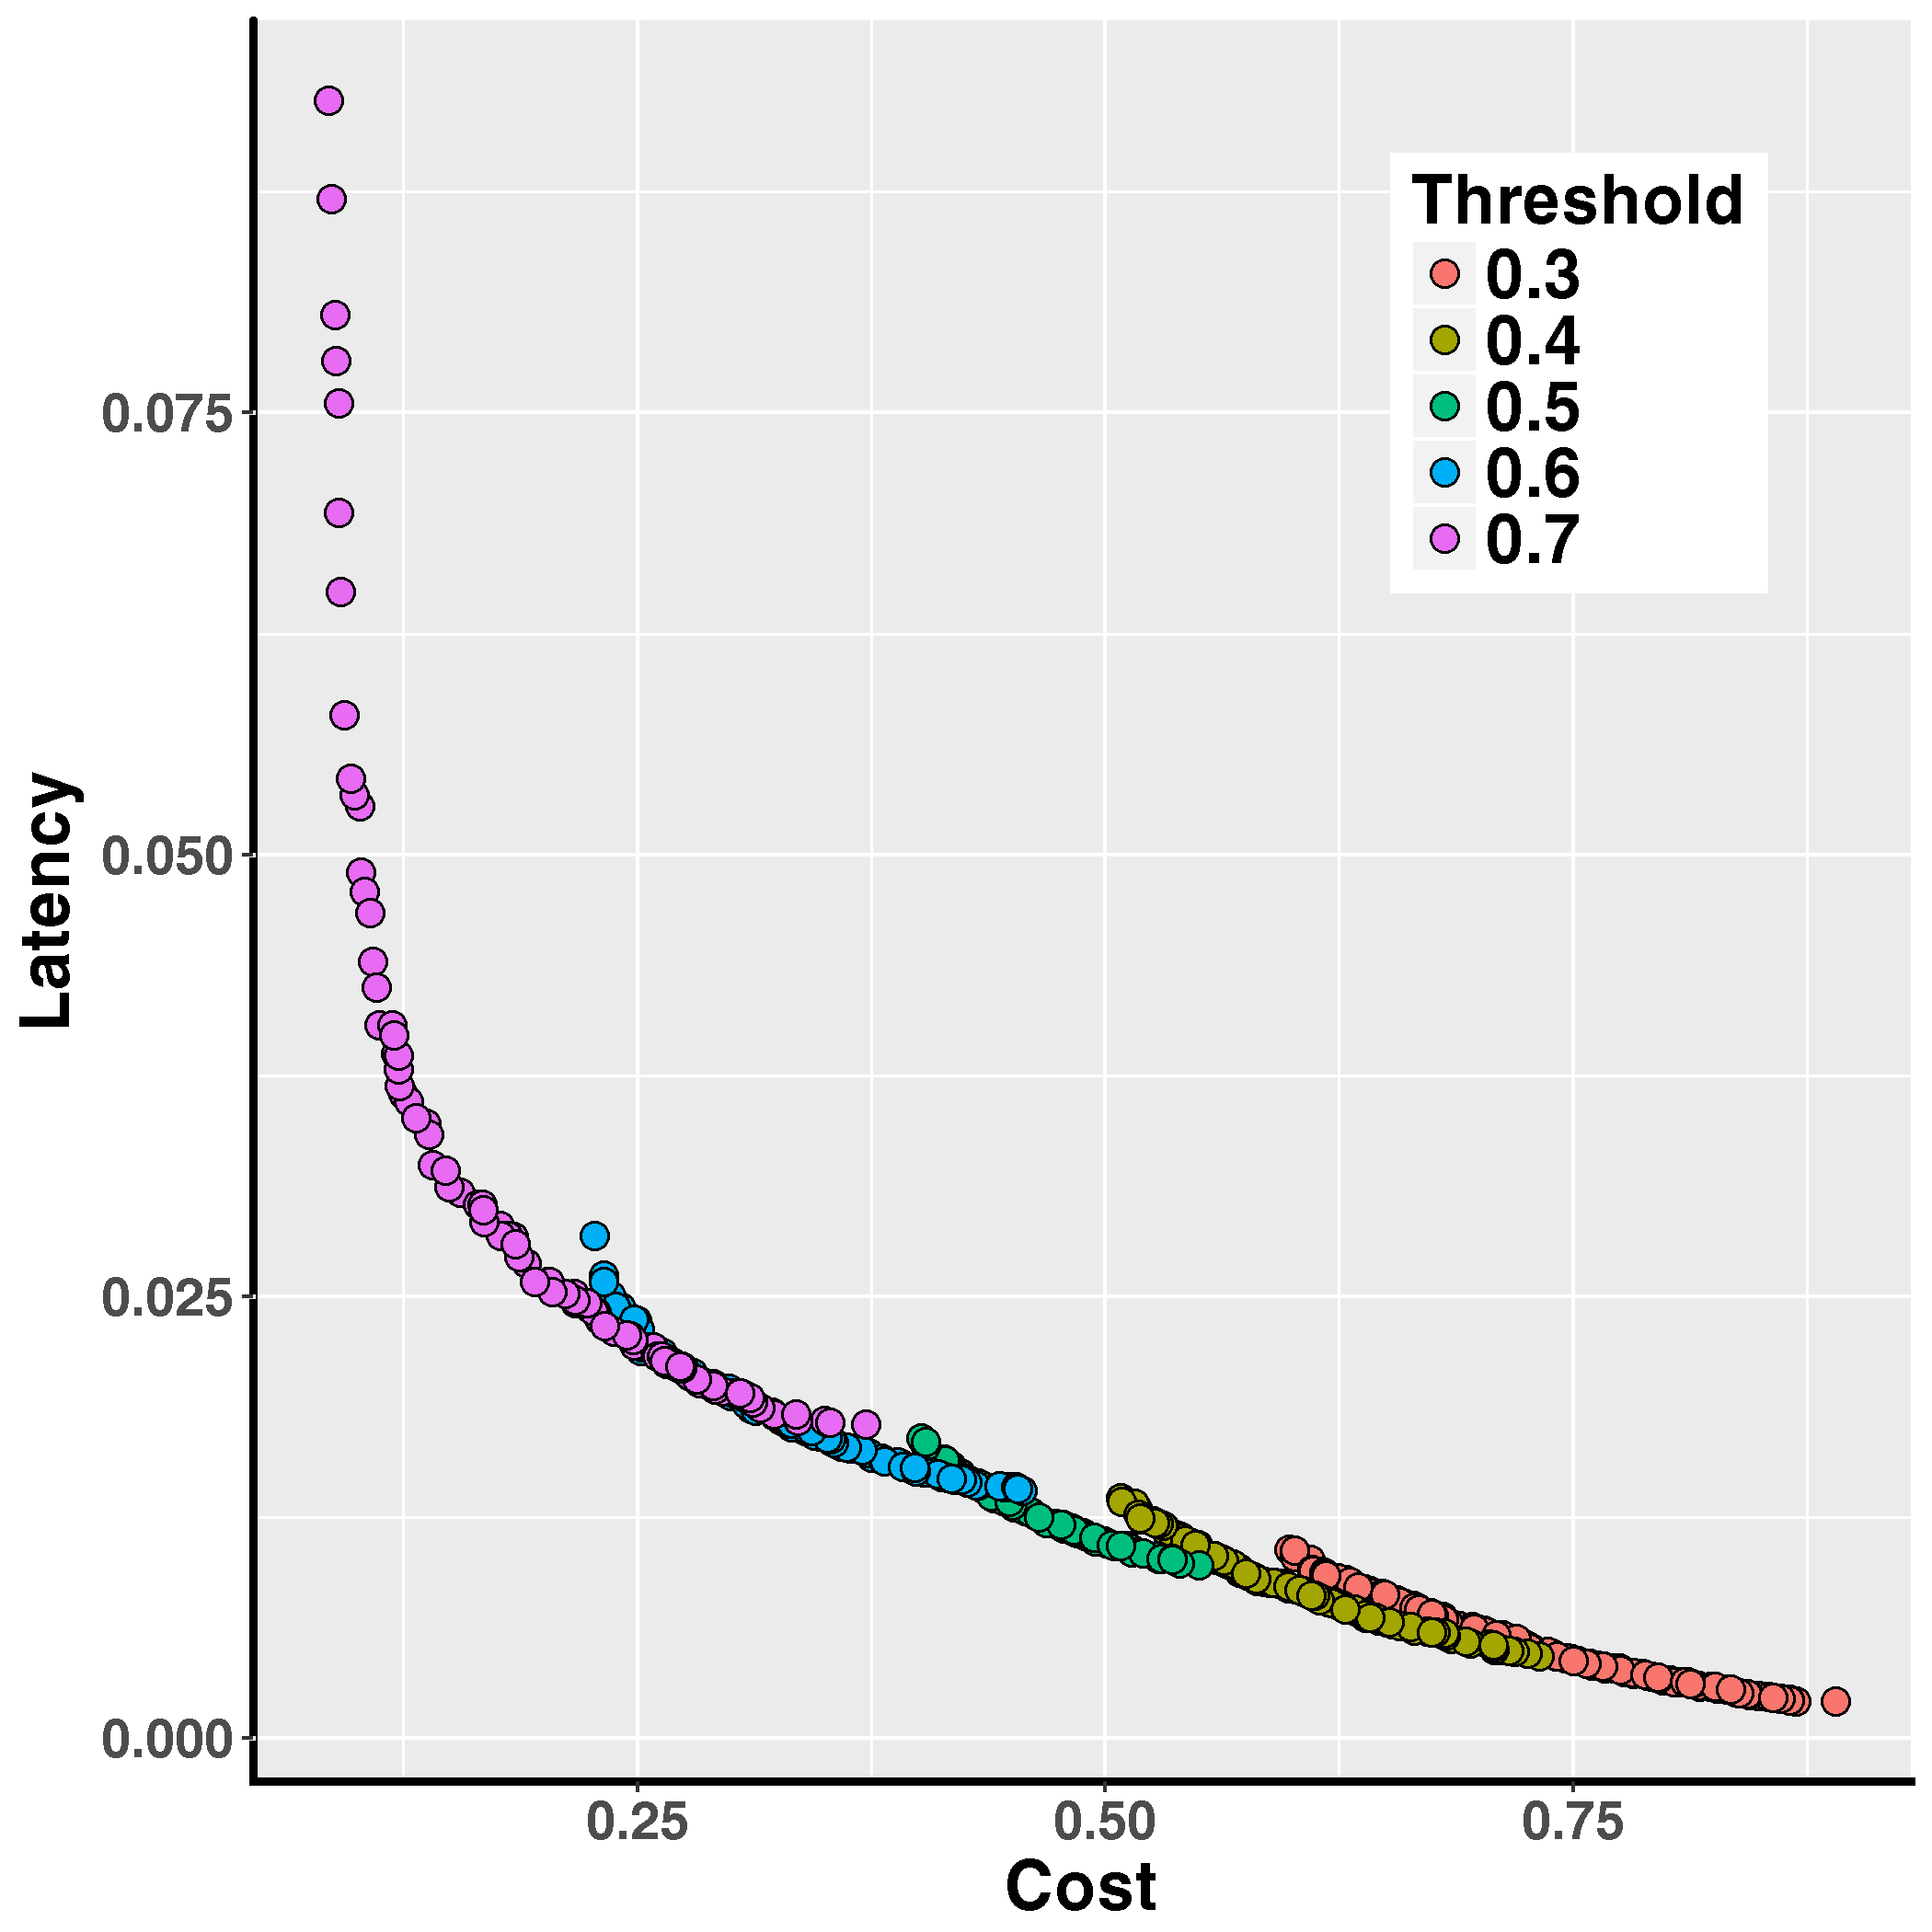
\includegraphics[width=\textwidth]{pics/static_threshold_problem_5.png}
    \caption{instance 5}
   \end{subfigure}
   \caption{Static Rounding Function Experiments:Solutions for Test instances 2 to 5 with different static threshold values}
   \label{fig:staticFunctions}
\end{figure}


\subsubsection{Dynamic Rounding Function}
In Section \ref{sec:dynamic}, three dynamic rounding functions are proposed. In this section, we evaluate the performances of these three rounding functions to find out which dynamic rounding function provides the best results.  The upper bound of dynamic threshold $u$ is set to 0.7 and the lower bound of dynamic threshold $l$ is set to 0.3. The results are compared in terms of mean IGD and HV.

\subsubsection{Comparison between Dynamic Rounding Functions}
\label{sec:expdy}
Table \ref{tab:hyperDynamic} shows the average performance of the three dynamic functions that are evaluated by HyperVolume.
The results indicate that the Reciprocal function outperformed other two dynamic functions in all test cases. This could be visually observed by plotting the best results (Figure \ref{fig:dynamicFunctions}).
Figure \ref{fig:dynamicFunctions} shows that the Reciprocal function slightly dominates the other two dynamic functions. However, the problem of the Reciprocal function is that it may miss some regions in the Pareto front, e.g. the regions between dashed-vertical lines of 0.45 and 0.55 in Figure \ref{fig:dynamicFunctions}. The gap is created because of the lack of uniformity (Figure \ref{fig:dynamic}).

\begin{figure}[h!]
   \centering
   \begin{subfigure}{0.49\linewidth}
       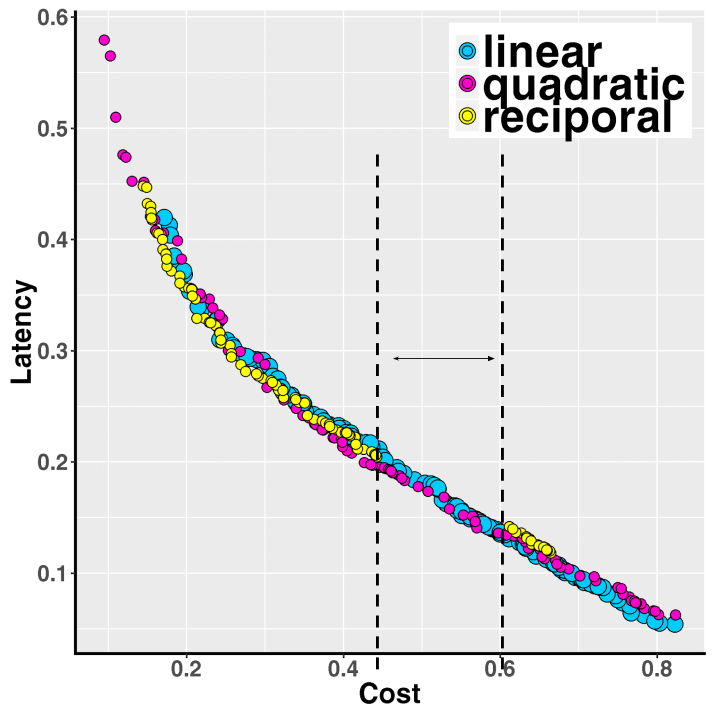
\includegraphics[width=\textwidth]{pics/dynamic_problem_2.png}
    \caption{instance 2}
   \end{subfigure}
   \begin{subfigure}{0.49\linewidth}
       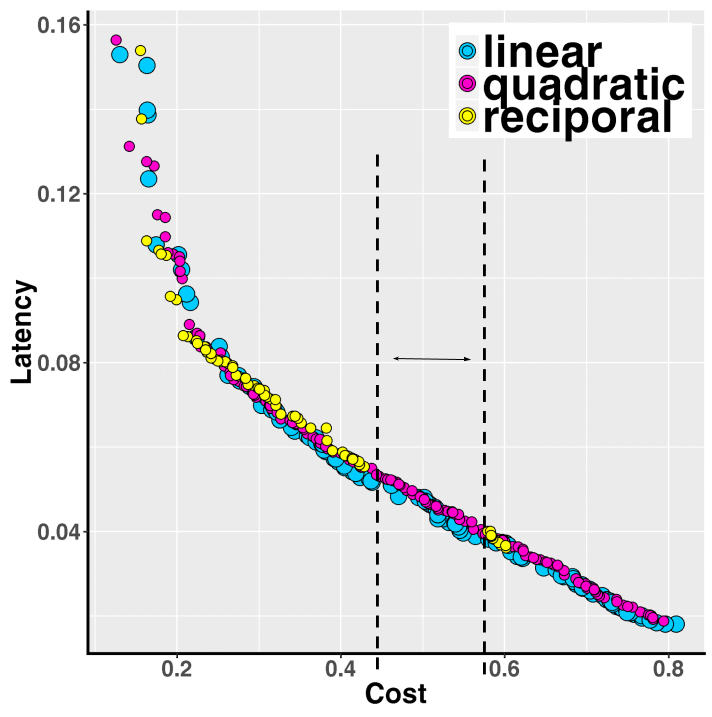
\includegraphics[width=\textwidth]{pics/dynamic_problem_3.png}
    \caption{instance 3}
   \end{subfigure}
   \begin{subfigure}{0.49\linewidth}
       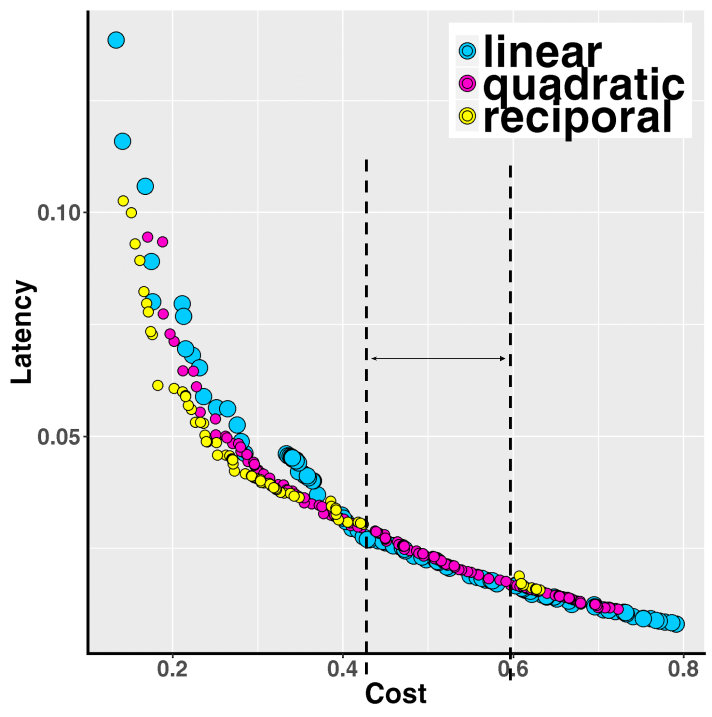
\includegraphics[width=\textwidth]{pics/dynamic_problem_4.png}
    \caption{instance 4}
   \end{subfigure}
   \begin{subfigure}{0.49\linewidth}
       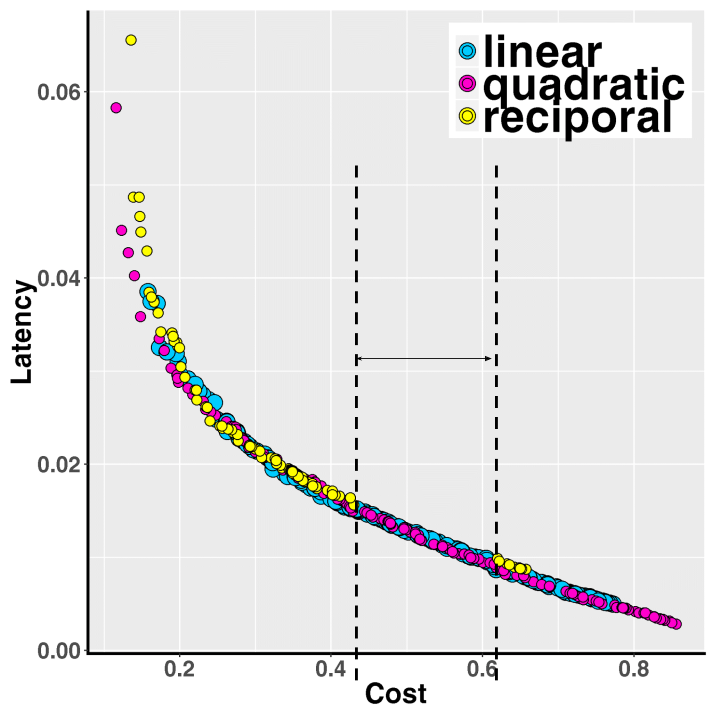
\includegraphics[width=\textwidth]{pics/dynamic_problem_5.png}
    \caption{instance 5}
   \end{subfigure}
   \caption{Dynamic Rounding Function Experiments : The non-dominated solutions among the sets obtained by 40 independent runs of BMOPSOCD with different dynamic functions. The dashed-vertical lines mark the missing solutions from the Reciprocal function.}
   \label{fig:dynamicFunctions}
\end{figure}


\begin{table}[H]
\centering
\footnotesize
\scalebox{0.8}{
\begin{tabular}{l|c|c|c}
\hline
          & \multicolumn{1}{l|}{Linear} & \multicolumn{1}{l|}{Quadratic} & \multicolumn{1}{l}{Reciprocal}  \\ \hline
instance 2 & 0.72 $\pm$ 0.011            & 0.73 $\pm$ 0.008               & \textbf{0.74 $\pm$ 0.013}    \\
instance 3 & 0.80 $\pm$ 0.012            & 0.81 $\pm$ 0.012               & \textbf{0.815 $\pm$ 0.013}    \\
instance 4 & 0.82 $\pm$ 0.012            & 0.86 $\pm$ 0.016               & \textbf{0.87 $\pm$ 0.014}   \\
instance 5 & 0.80 $\pm$ 0.014            & 0.85 $\pm$ 0.023               & \textbf{0.86 $\pm$ 0.020}   \\ \hline
\end{tabular}}
\caption{The mean and standard deviation of the HyperVolume values over the 40 independent runs}
\label{tab:hyperDynamic}

\end{table}

The experimental results \ref{tab:hyperDynamic} show that in terms of convergence, the Reciprocal function produces the best result. 
However, it also shows the disadvantage of the Reciprocal function, which cannot provide a non-dominated set that covers the entire Pareto front. 
In contrast, the Quadratic function performs
slightly worse in convergence but obtains a good-coverage non-dominated set. The Linear function is dominated by Quadratic function in both aspects.

The better convergence with the Reciprocal function can be explained, as there is a minor change in threshold in the most generations and the swarm has a longer time to search along the same direction. However, with the Linear and Quadratic function, the constant changing in direction does not give the algorithm enough time to find a good solution.

Between the Quadratic function and the Linear function, their changing rate of threshold value are different: the Linear function changes equally, while the Quadratic function changes little at the beginning and then become larger. As the swarm searches the low-cost region (as the threshold starts decreasing from 0.7) and moves to high-cost region, it has more time to search in the low-cost region with the Quadratic function. This is the key reason that the performance of the Quadratic function is better than that of Linear function, because we have observed that the number of solutions in the low-cost region is much smaller than in the high-cost region, as shown in Figure \ref{fig:staticFunctions}, the low-cost regions are quite sparse compare with the low-latency regions. Therefore, it is reasonable to give the algorithm more time to search the low-cost region, while, in the low-latency region, the algorithm can spend much less effort because the solutions are rich. In general, algorithm with the Quadratic function obtains better solutions in the low-cost region than with Linear function.

From table \ref{tab:hyperDynamic}, in terms of HyperVolume, the Reciprocal function has the best performance. However, we can observe that the Reciprocal function cannot provide a good coverage of the Pareto front in Figure \ref{fig:dynamicFunctions}. That is, the Reciprocal function missed many useful solutions because it lacks uniformity. Therefore, we cannot determine which algorithm is better solely 
depending on the HyperVolume values. We conclude that the Quadratic function performances the best. Although the Quadratic function is worse than the Reciprocal function in terms of HyperVolume value, the disadvantage of Reciprocal function cannot be ignored.

\subsubsection{Stepped Rounding Function}
We study the performance of the Stepped rounding function in this experiment. The upper and lower bound $u$ and $l$ are set to 0.7 and 0.3 respectively. The interval is set to 10 generations. The results are compared with dynamic functions.

\subsubsection{Results for the Stepped Rounding function}
We compared the performance of the Stepped rounding function with the Reciprocal rounding function. The averages of HV of three rounding functions are shown in Table \ref{tab:transfercomp}. Table \ref{tab:transfercomp} shows that in terms of HV, Reciprocal function performs better than the Stepped threshold approach in most cases.
However, Figure \ref{fig:transfer} shows that the Stepped rounding function dominates in instance 3 and has better diversity in instance 4.
The results indicate that the Stepped rounding function could provide a uniformly distributed non-dominated set.
Overall, the performance of the Stepped rounding function is very close to the Reciprocal function and almost the same with the Quadratic function.

\begin{table}[]
\centering
\footnotesize
\scalebox{0.75}{
\begin{tabular}{l|c|c}
\hline
                                                                                                            & Reciprocal                                                                                                                                     & Stepped                                                                                                                     \\ \hline
\multicolumn{1}{c|}{\begin{tabular}[c]{@{}c@{}}instance 2\\ instance 3\\ instance 4\\ instance 5\end{tabular}} & \begin{tabular}[c]{@{}c@{}}\textbf{0.74 $\pm$ 0.013} \\ 0.815 $\pm$ 0.013\\ \textbf{0.87 $\pm$ 0.014} \\ \textbf{0.86 $\pm$ 0.020}  \end{tabular} & \begin{tabular}[c]{@{}c@{}}0.72 $\pm$ 0.011\\  \textbf{0.83 $\pm$ 0.014} \\ 0.85 $\pm$ 0.014\\ 0.85 $\pm$ 0.022\end{tabular} \\ \hline
\end{tabular}}
\caption{A comparison between the Reciprocal function and the Stepped function, the mean and standard deviation of HyperVolume values over the 40 independent runs}
\label{tab:transfercomp}
\end{table}



\begin{figure}[h!]
   \centering
   \begin{subfigure}{0.49\linewidth}
       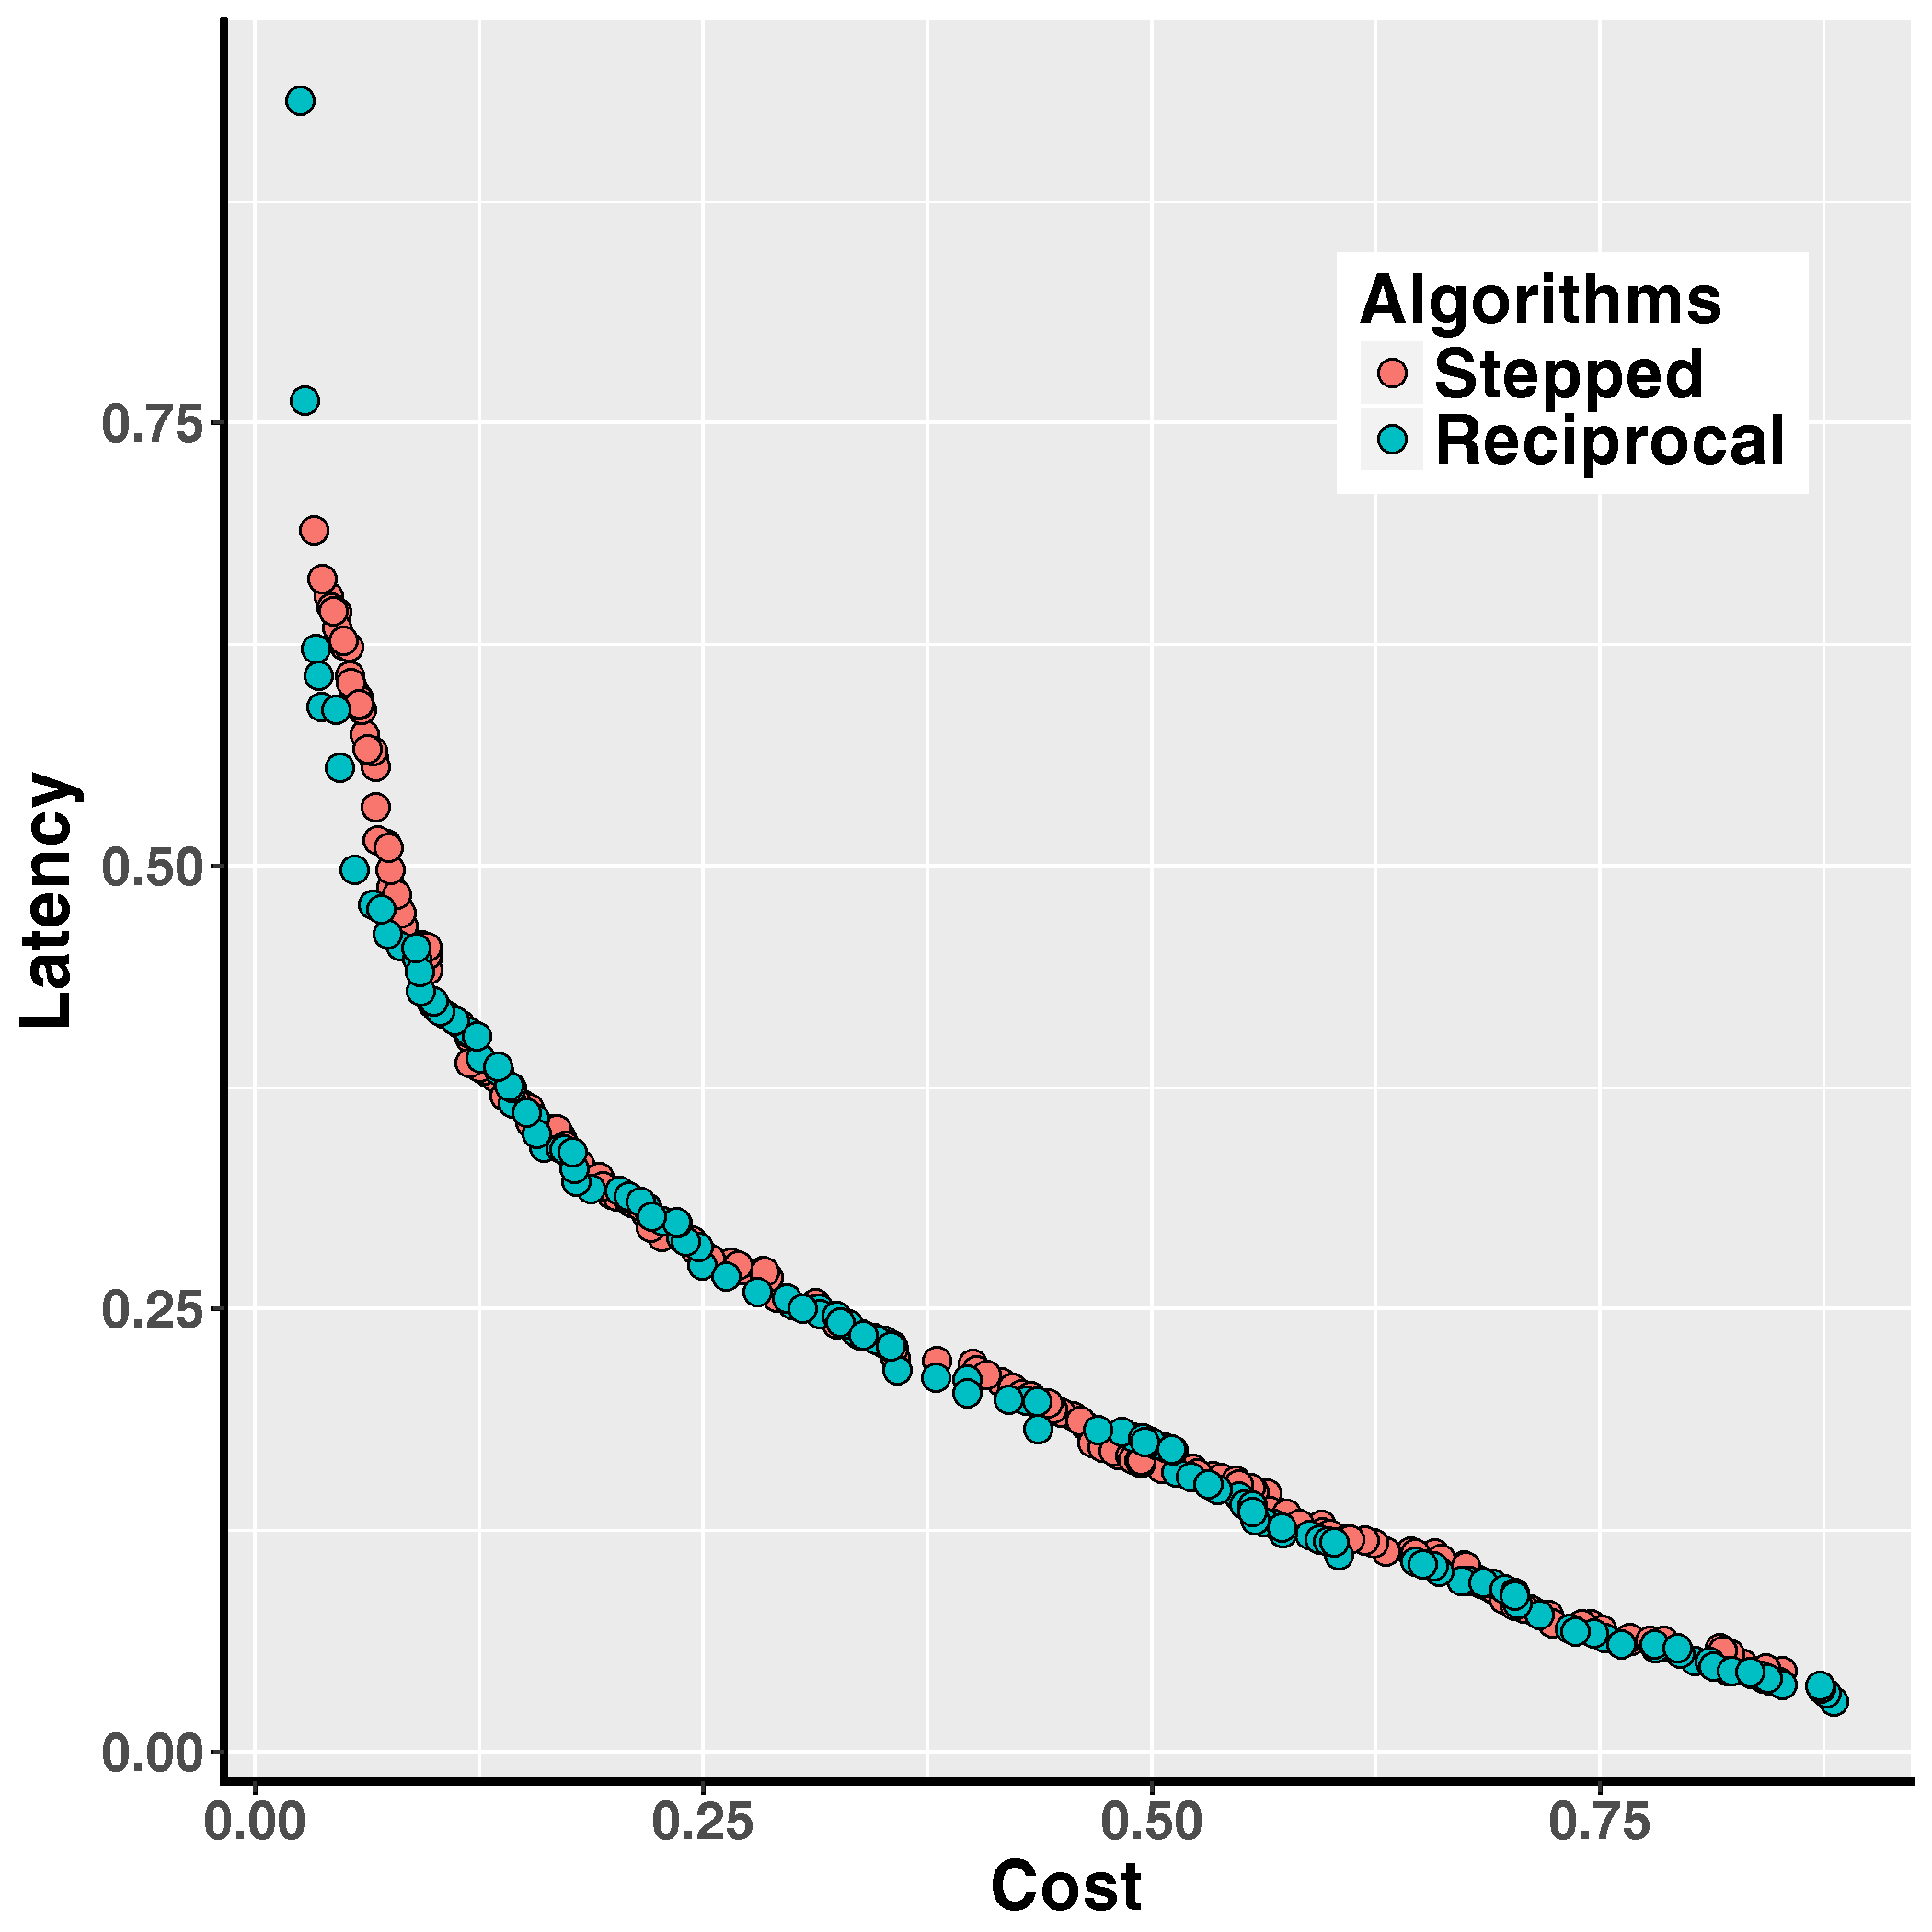
\includegraphics[width=\textwidth]{pics/transfer_problem2.png}
    \caption{instance 2}
   \end{subfigure}
   \begin{subfigure}{0.49\linewidth}
       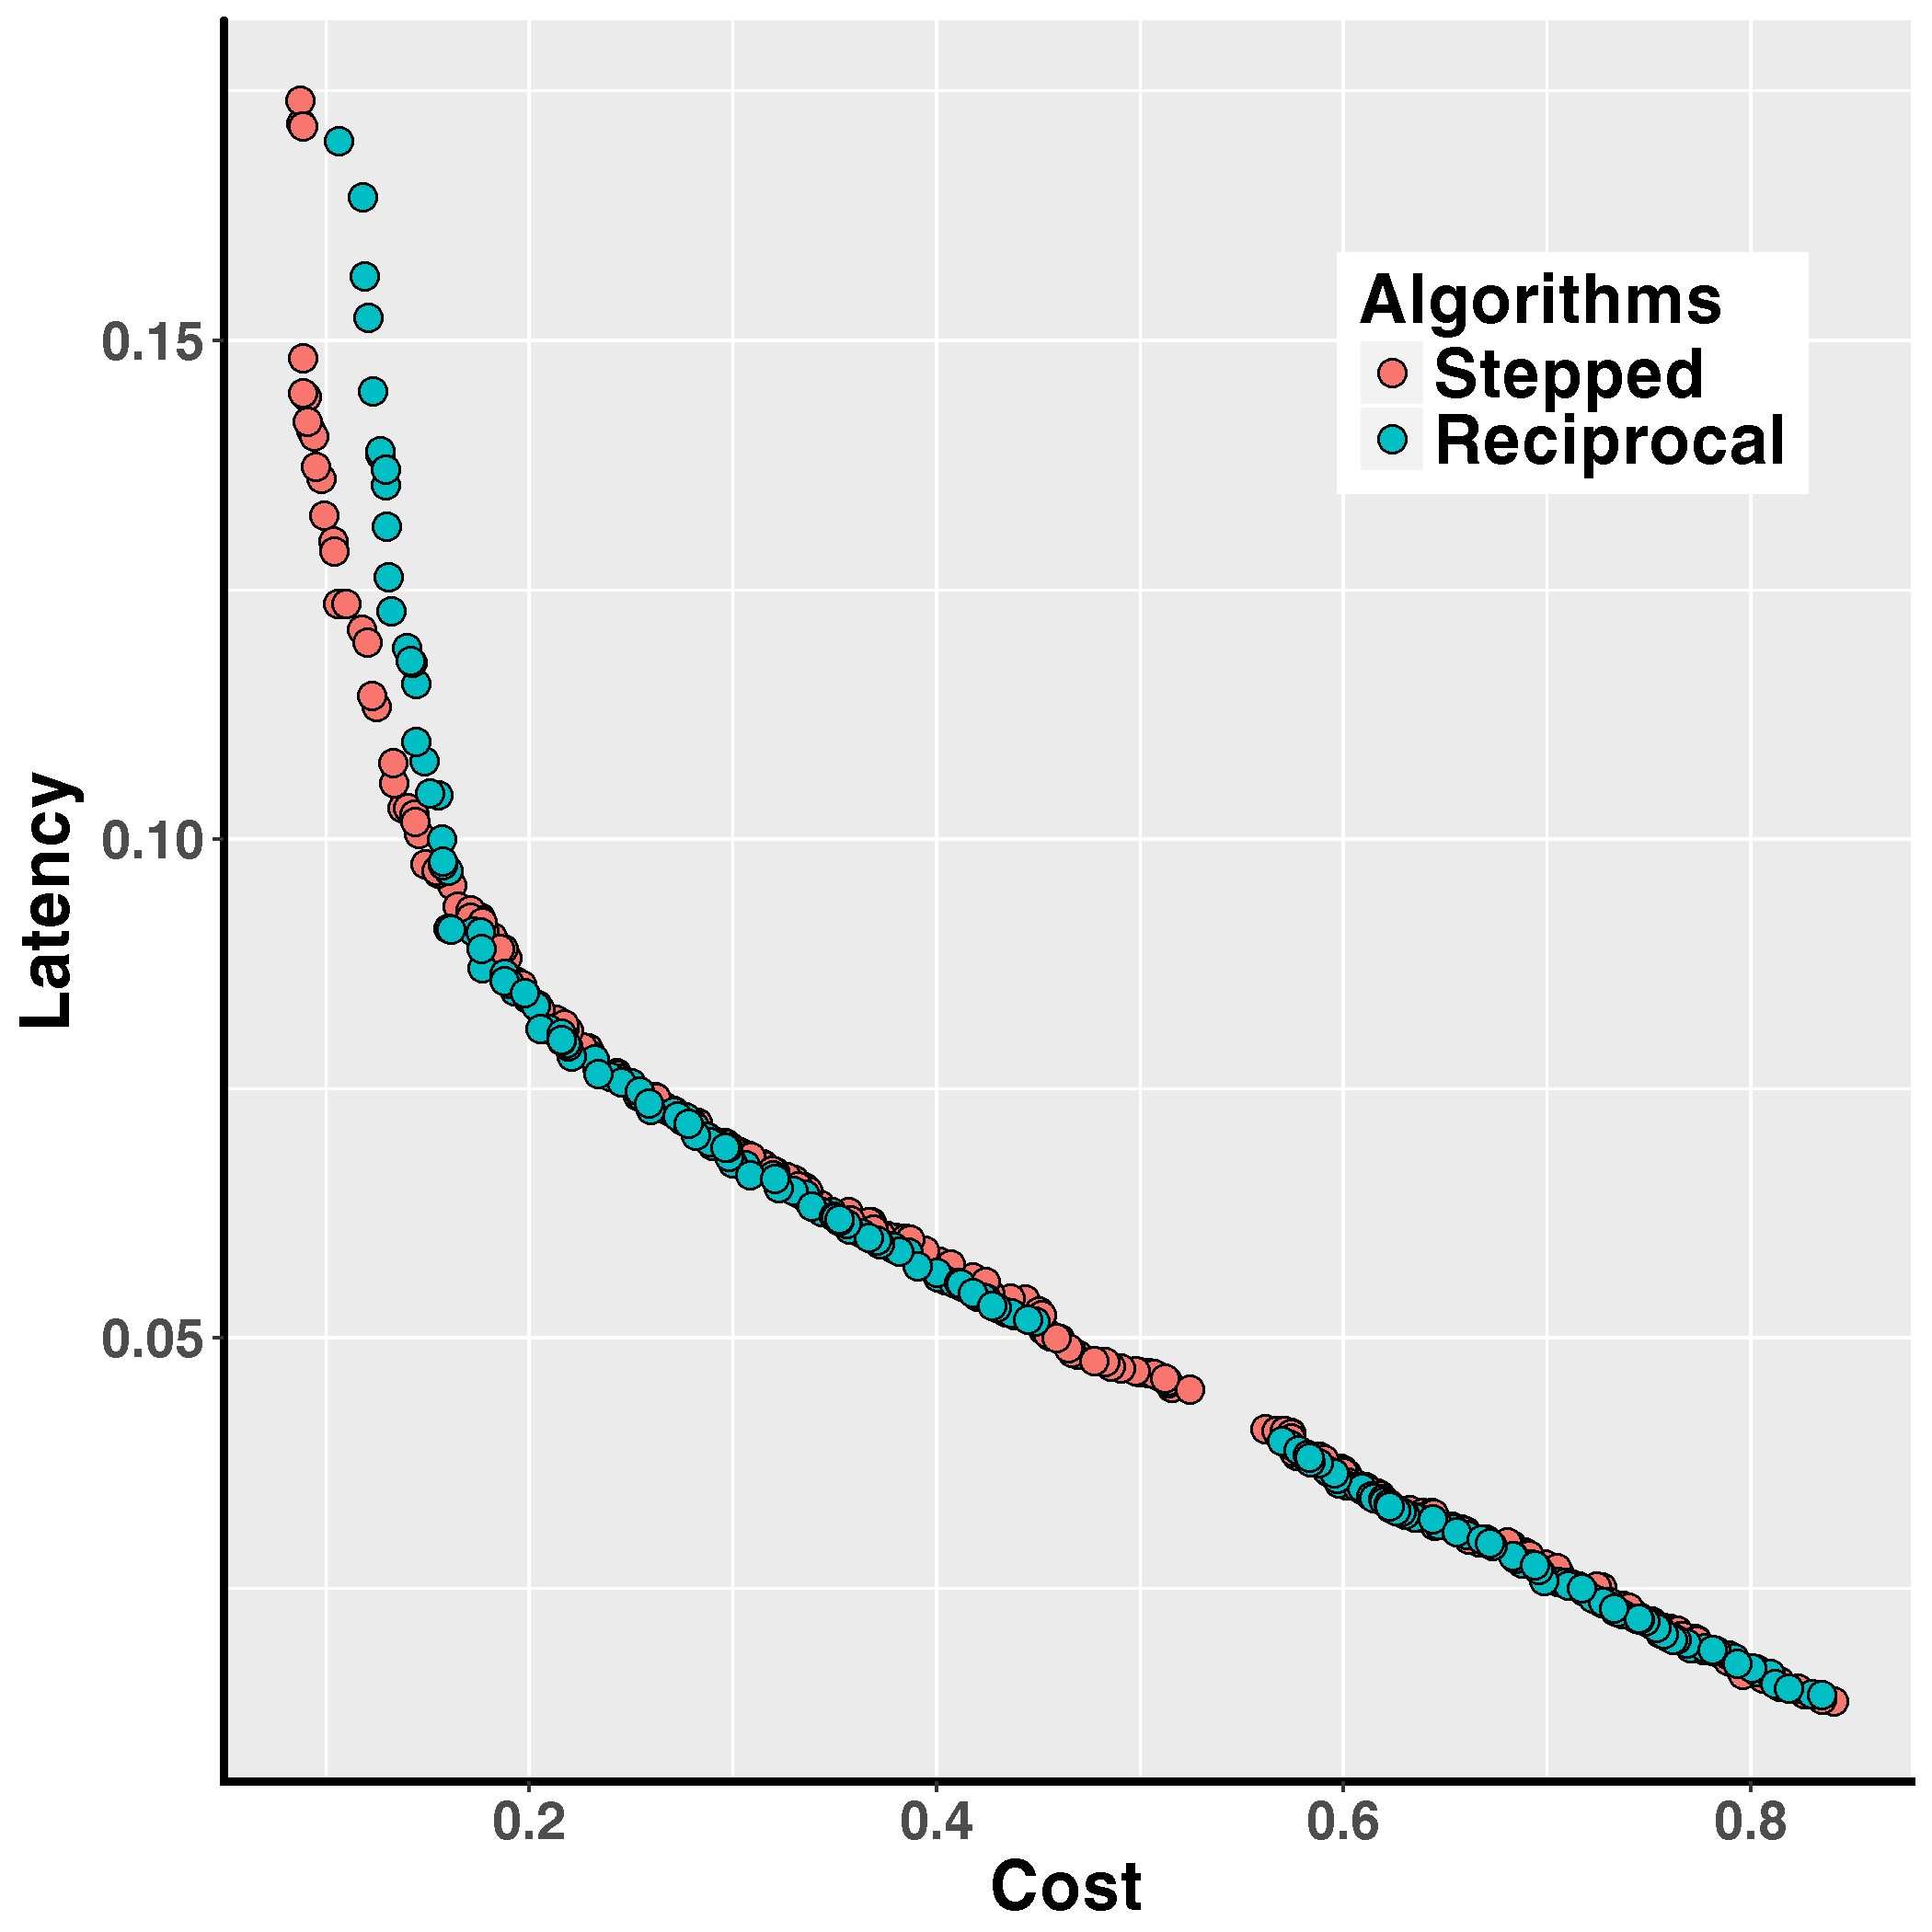
\includegraphics[width=\textwidth]{pics/transfer_problem3.png}
    \caption{instance 3}
   \end{subfigure}
   \begin{subfigure}{0.49\linewidth}
       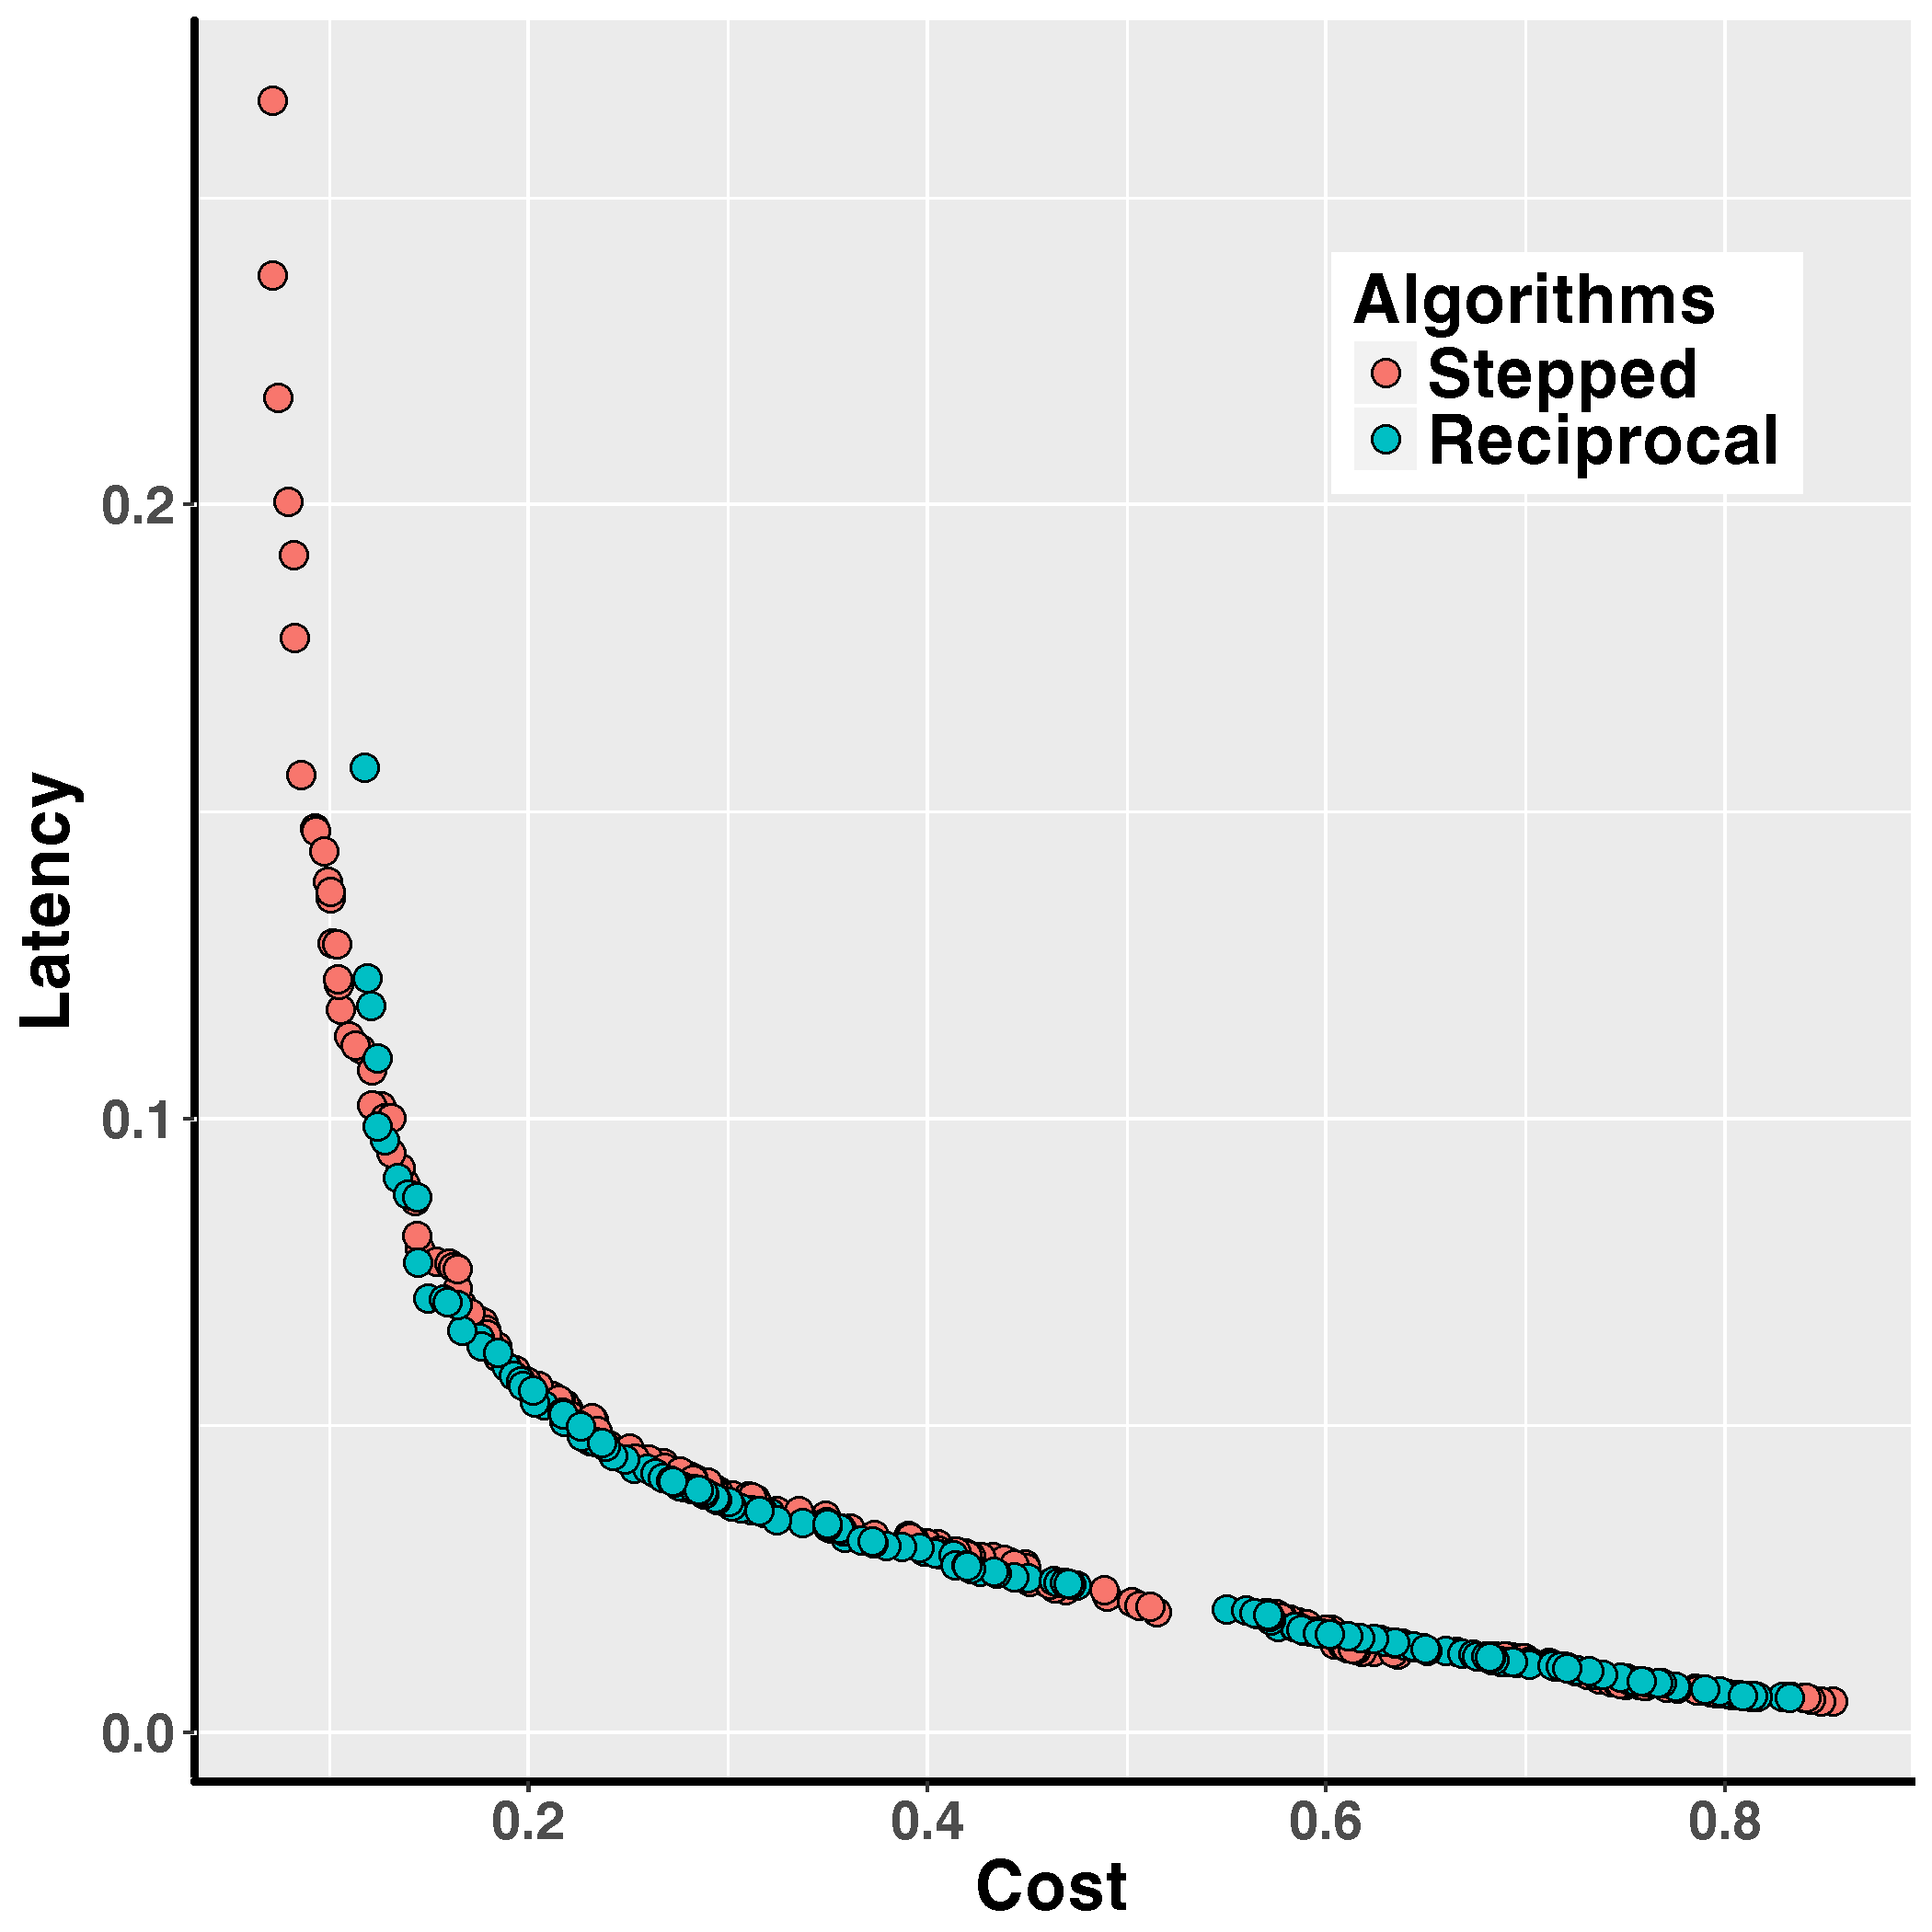
\includegraphics[width=\textwidth]{pics/transfer_problem4.png}
    \caption{instance 4}
   \end{subfigure}
   \begin{subfigure}{0.49\linewidth}
       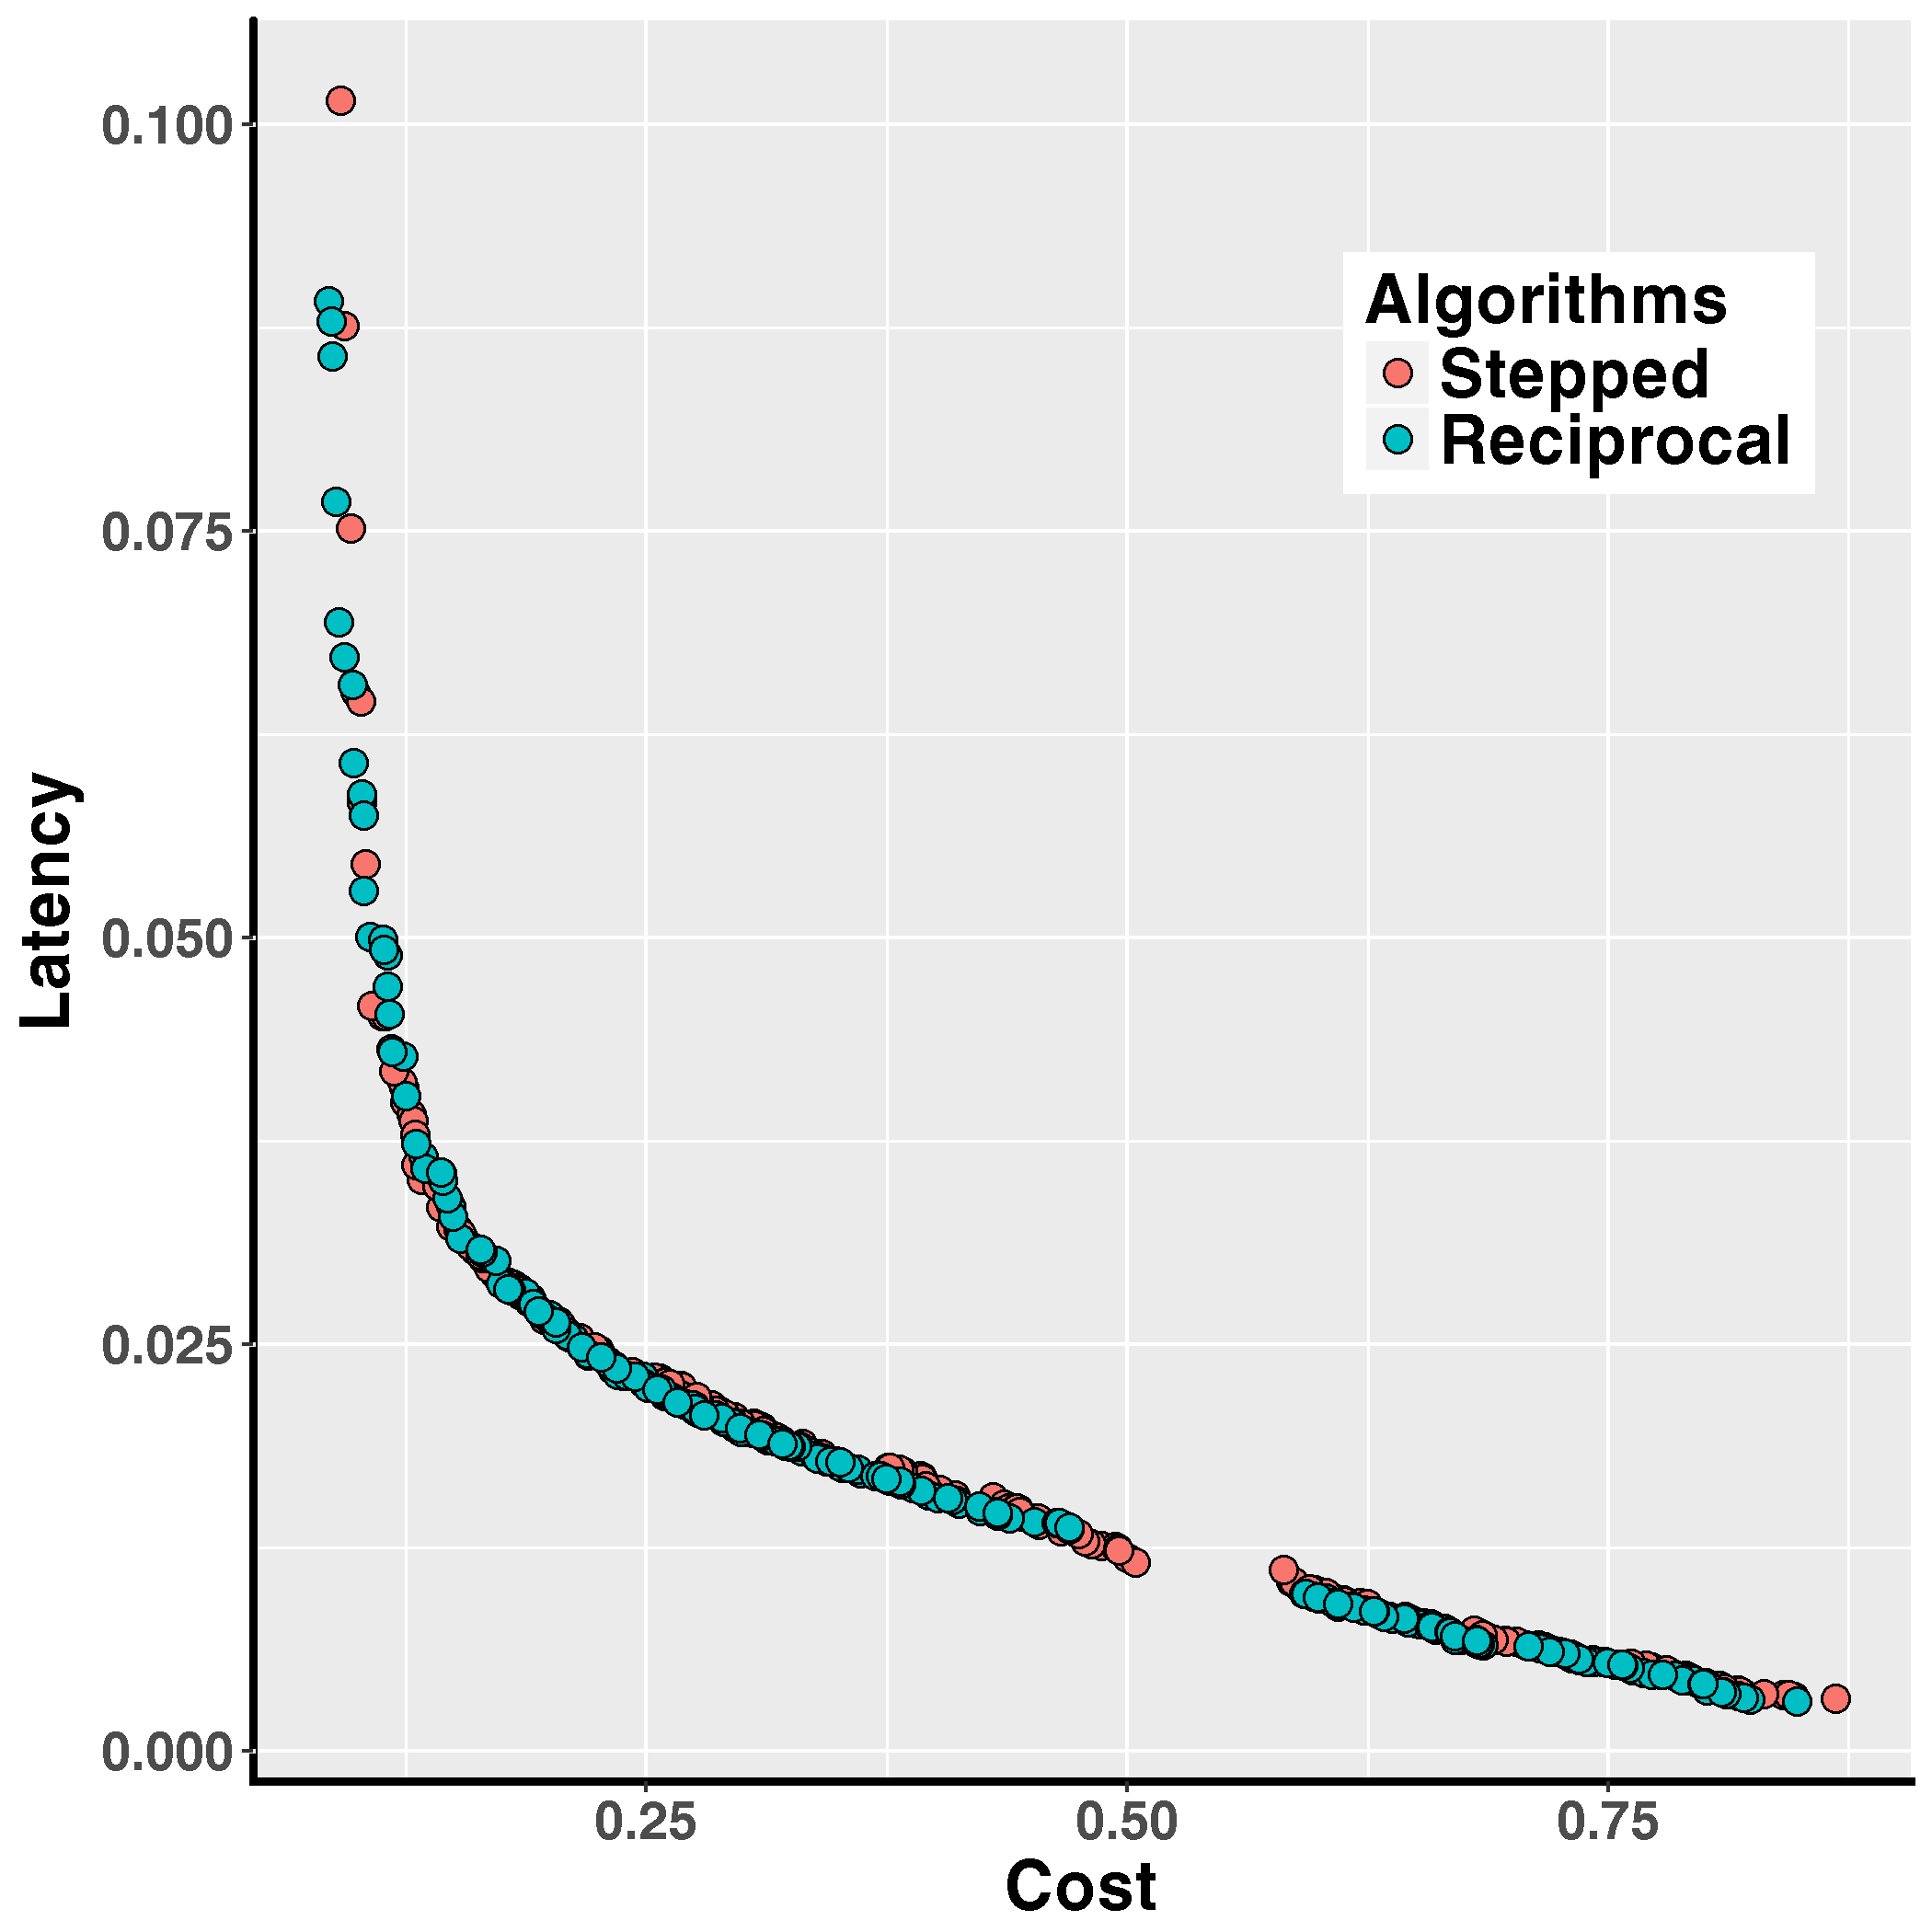
\includegraphics[width=\textwidth]{pics/transfer_problem5.png}
    \caption{instance 5}
   \end{subfigure}
   \caption{The Stepped Rounding Function Experiments: The non-dominated solutions among the sets obtained by 40 independent runs of the Stepped function and the Reciprocal
   function}
   \label{fig:transfer}
\end{figure}

\vspace{-3 mm}
\subsubsection{Combination of Static Function}
In this experiment, we combined all solutions from 5 static rounding functions mentioned in Section \ref{sec:static_exp} and applied
a fast non-dominated sorting over it. The performance is compared with the Reciprocal rounding function in Figure \ref{fig:combination}.
As the figure shows, the combined non-dominated set dominates all the other results in all the test instances. The solutions are not only diverse but also uniformly distributed.
However, the method takes five times longer than using the Reciprocal function.

\begin{figure}[h!]
   \centering
   \begin{subfigure}{0.49\linewidth}
       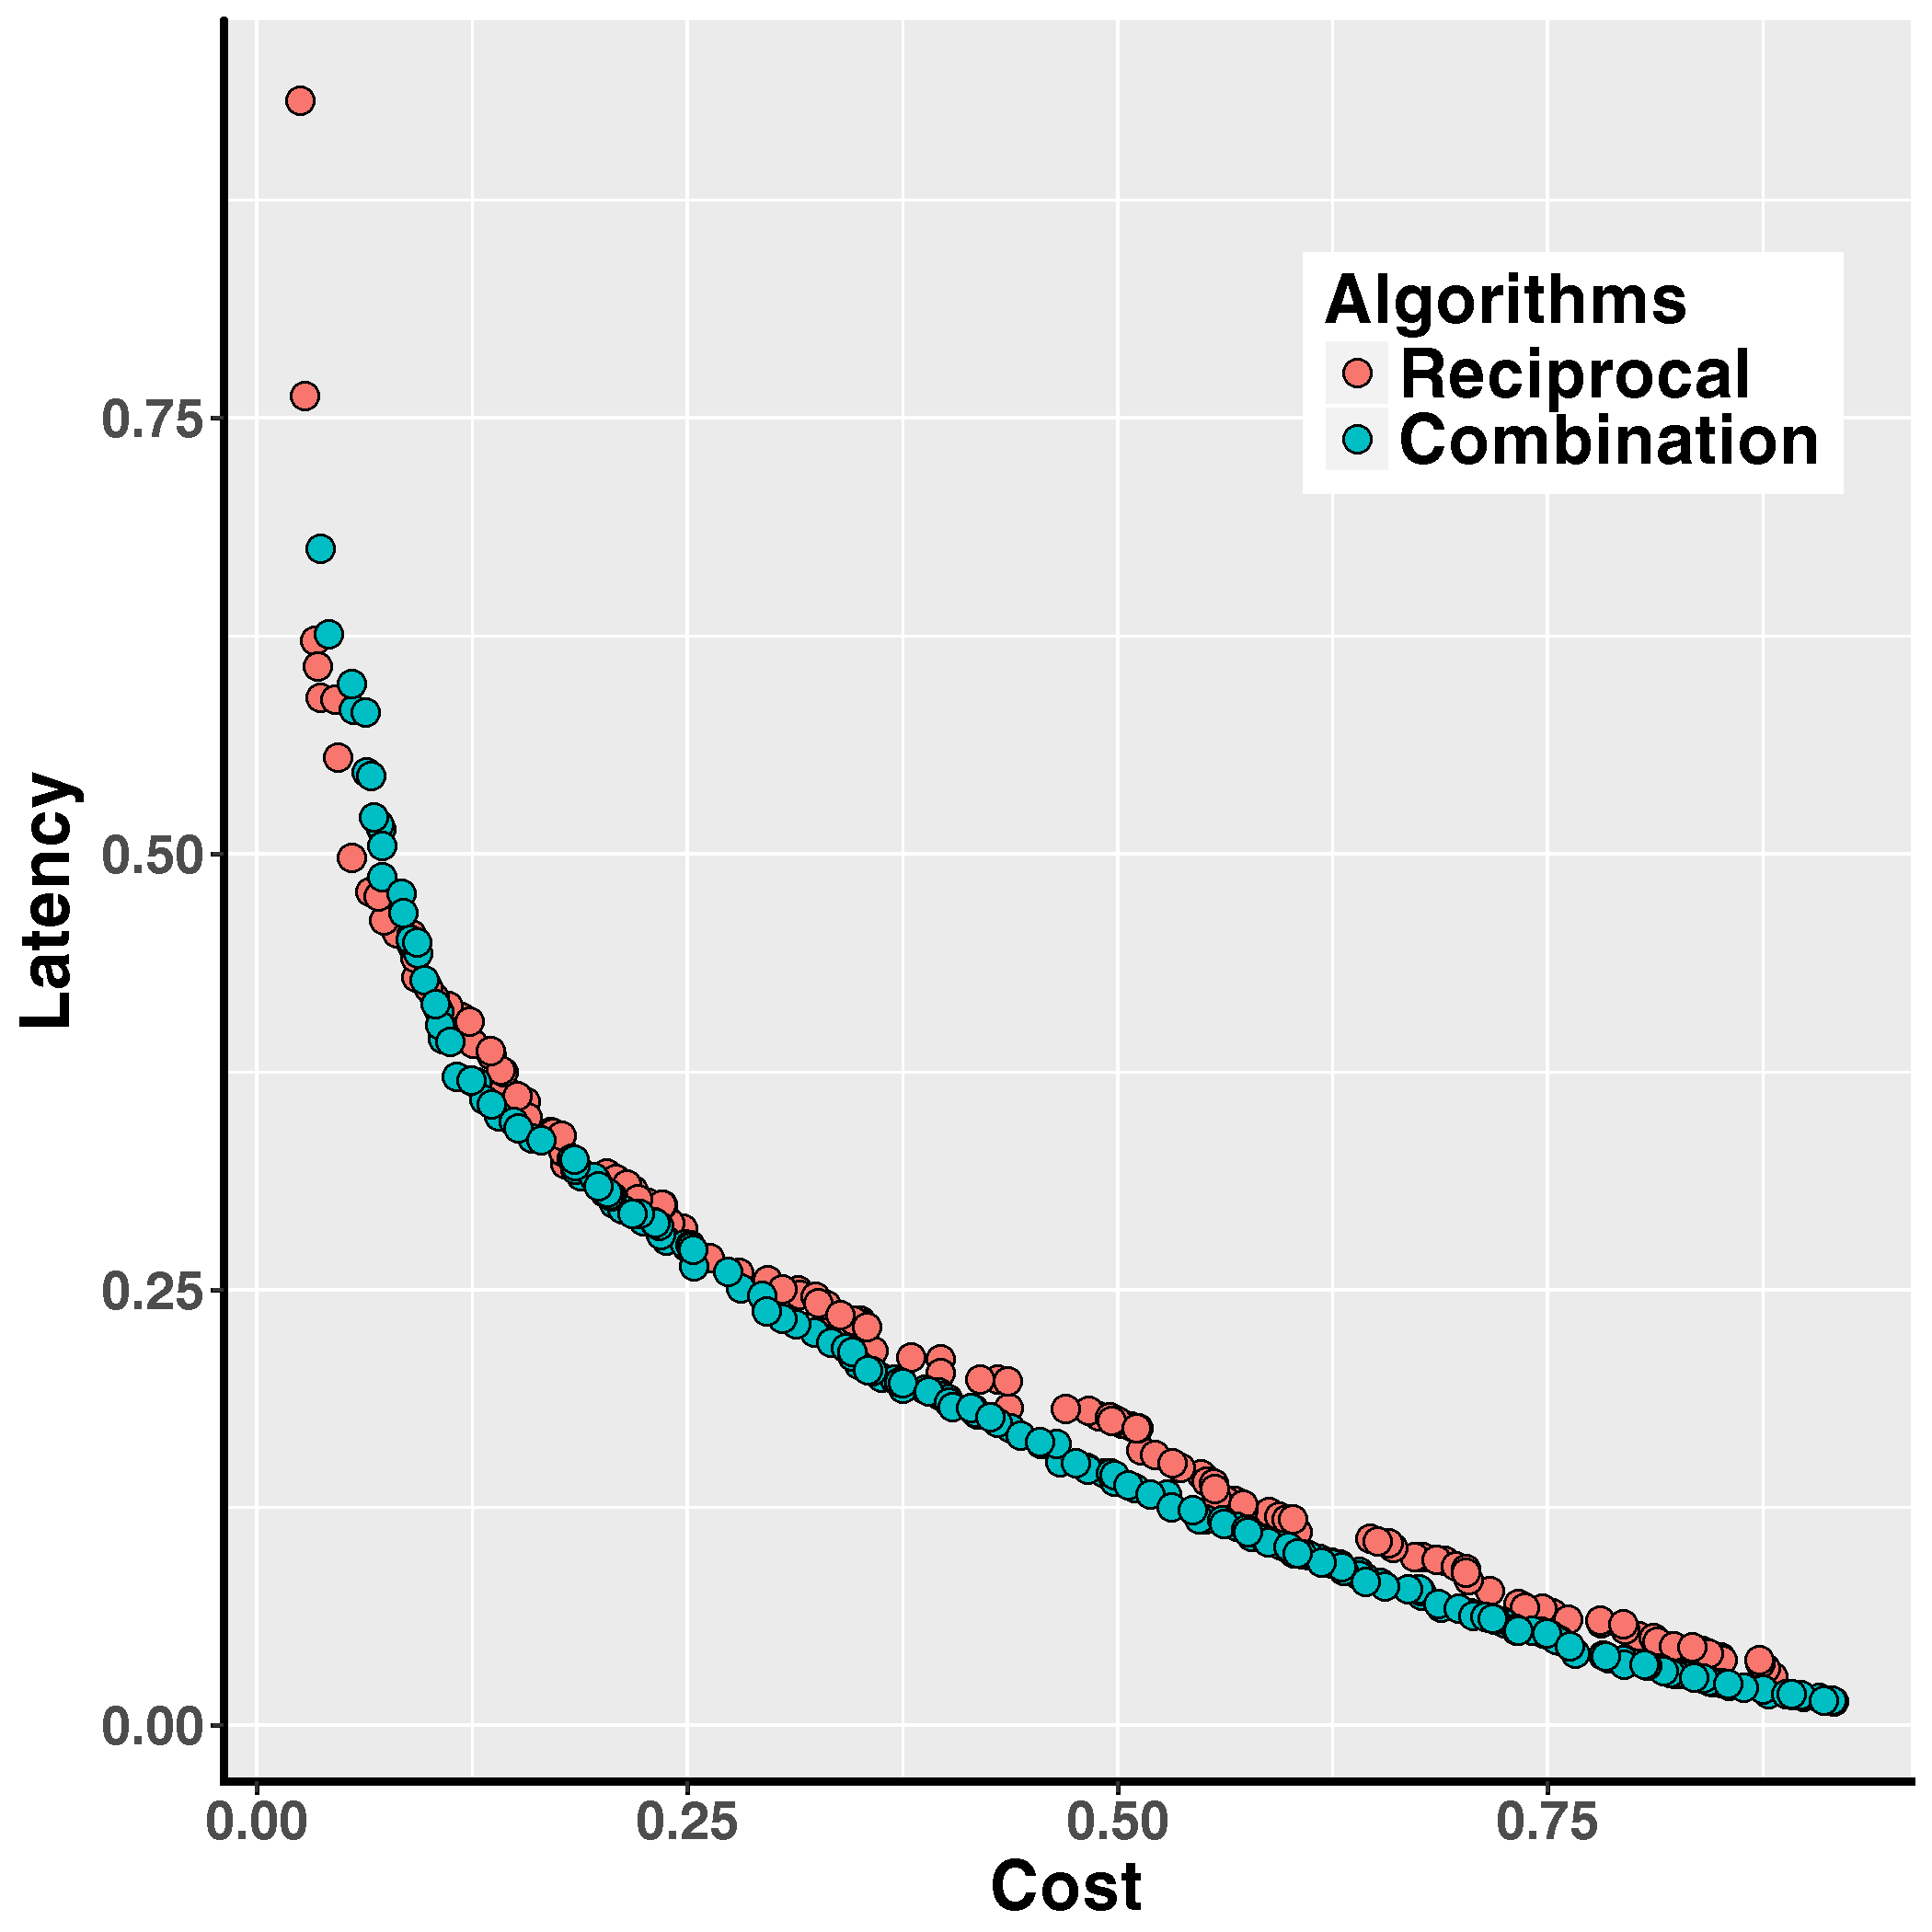
\includegraphics[width=\textwidth]{pics/combination_problem2.png}
    \caption{instance 2}
   \end{subfigure}
   \begin{subfigure}{0.49\linewidth}
       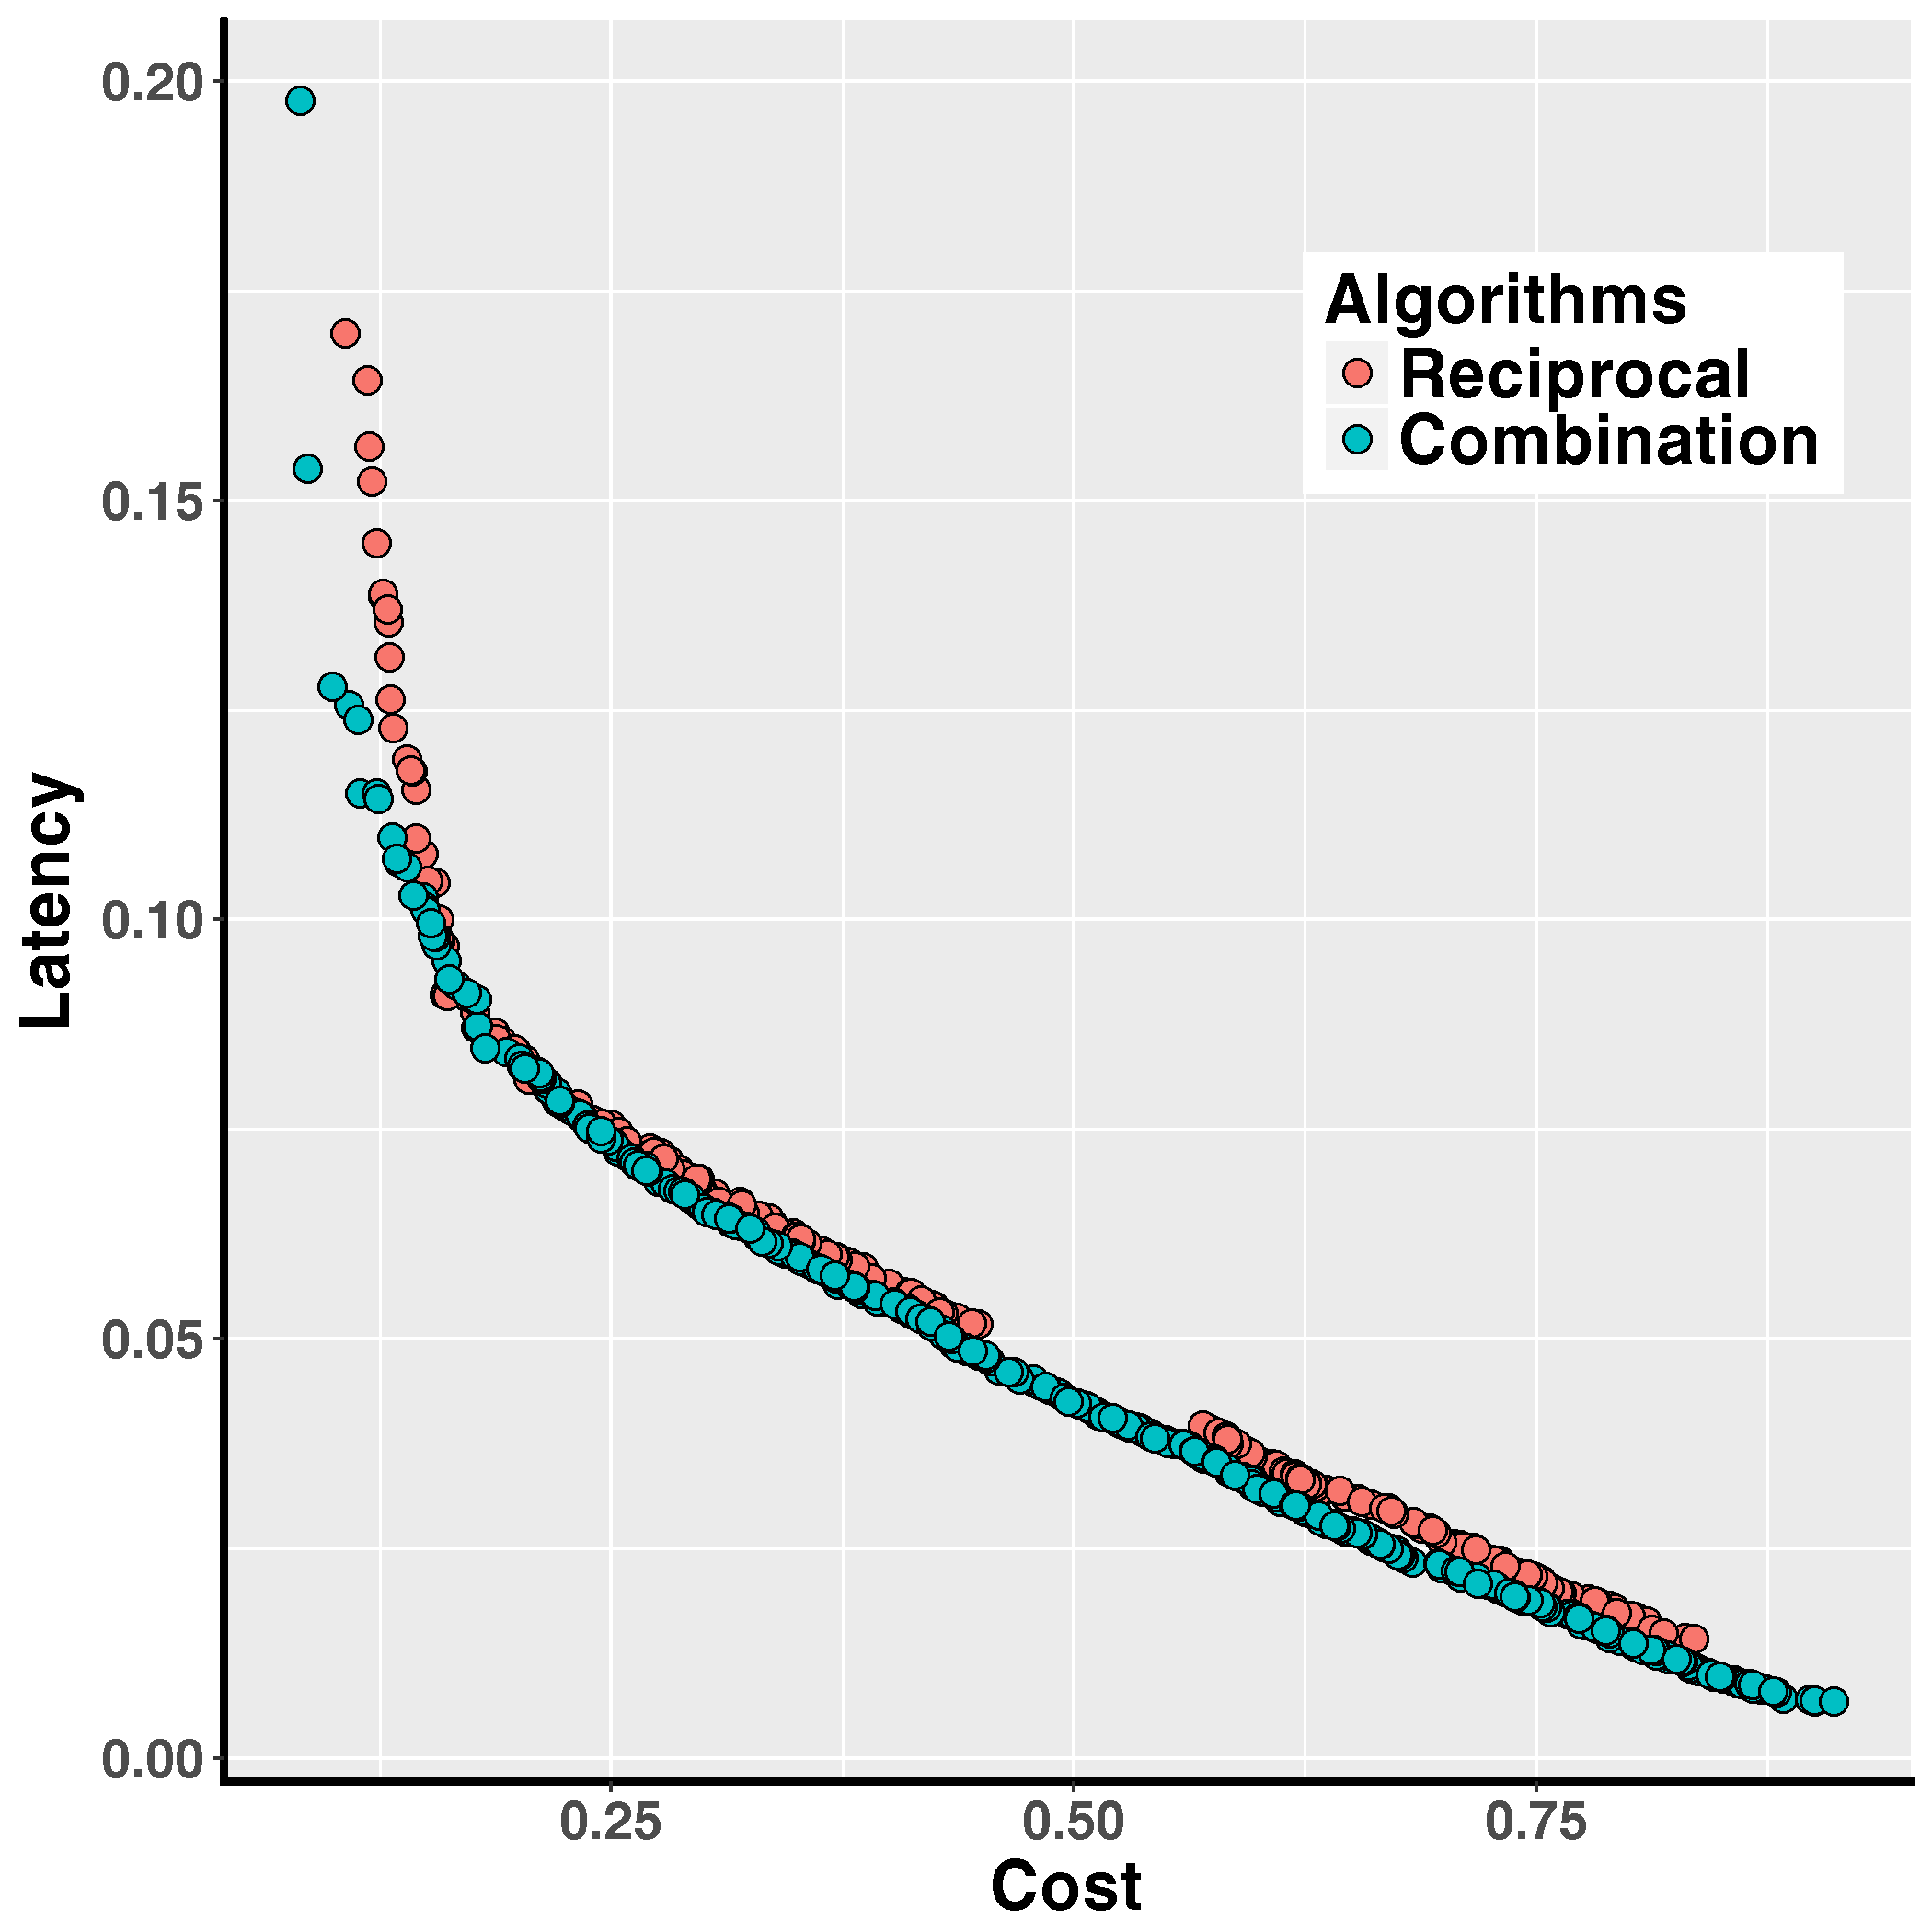
\includegraphics[width=\textwidth]{pics/combination_problem3.png}
    \caption{instance 3}
   \end{subfigure}
   \begin{subfigure}{0.49\linewidth}
       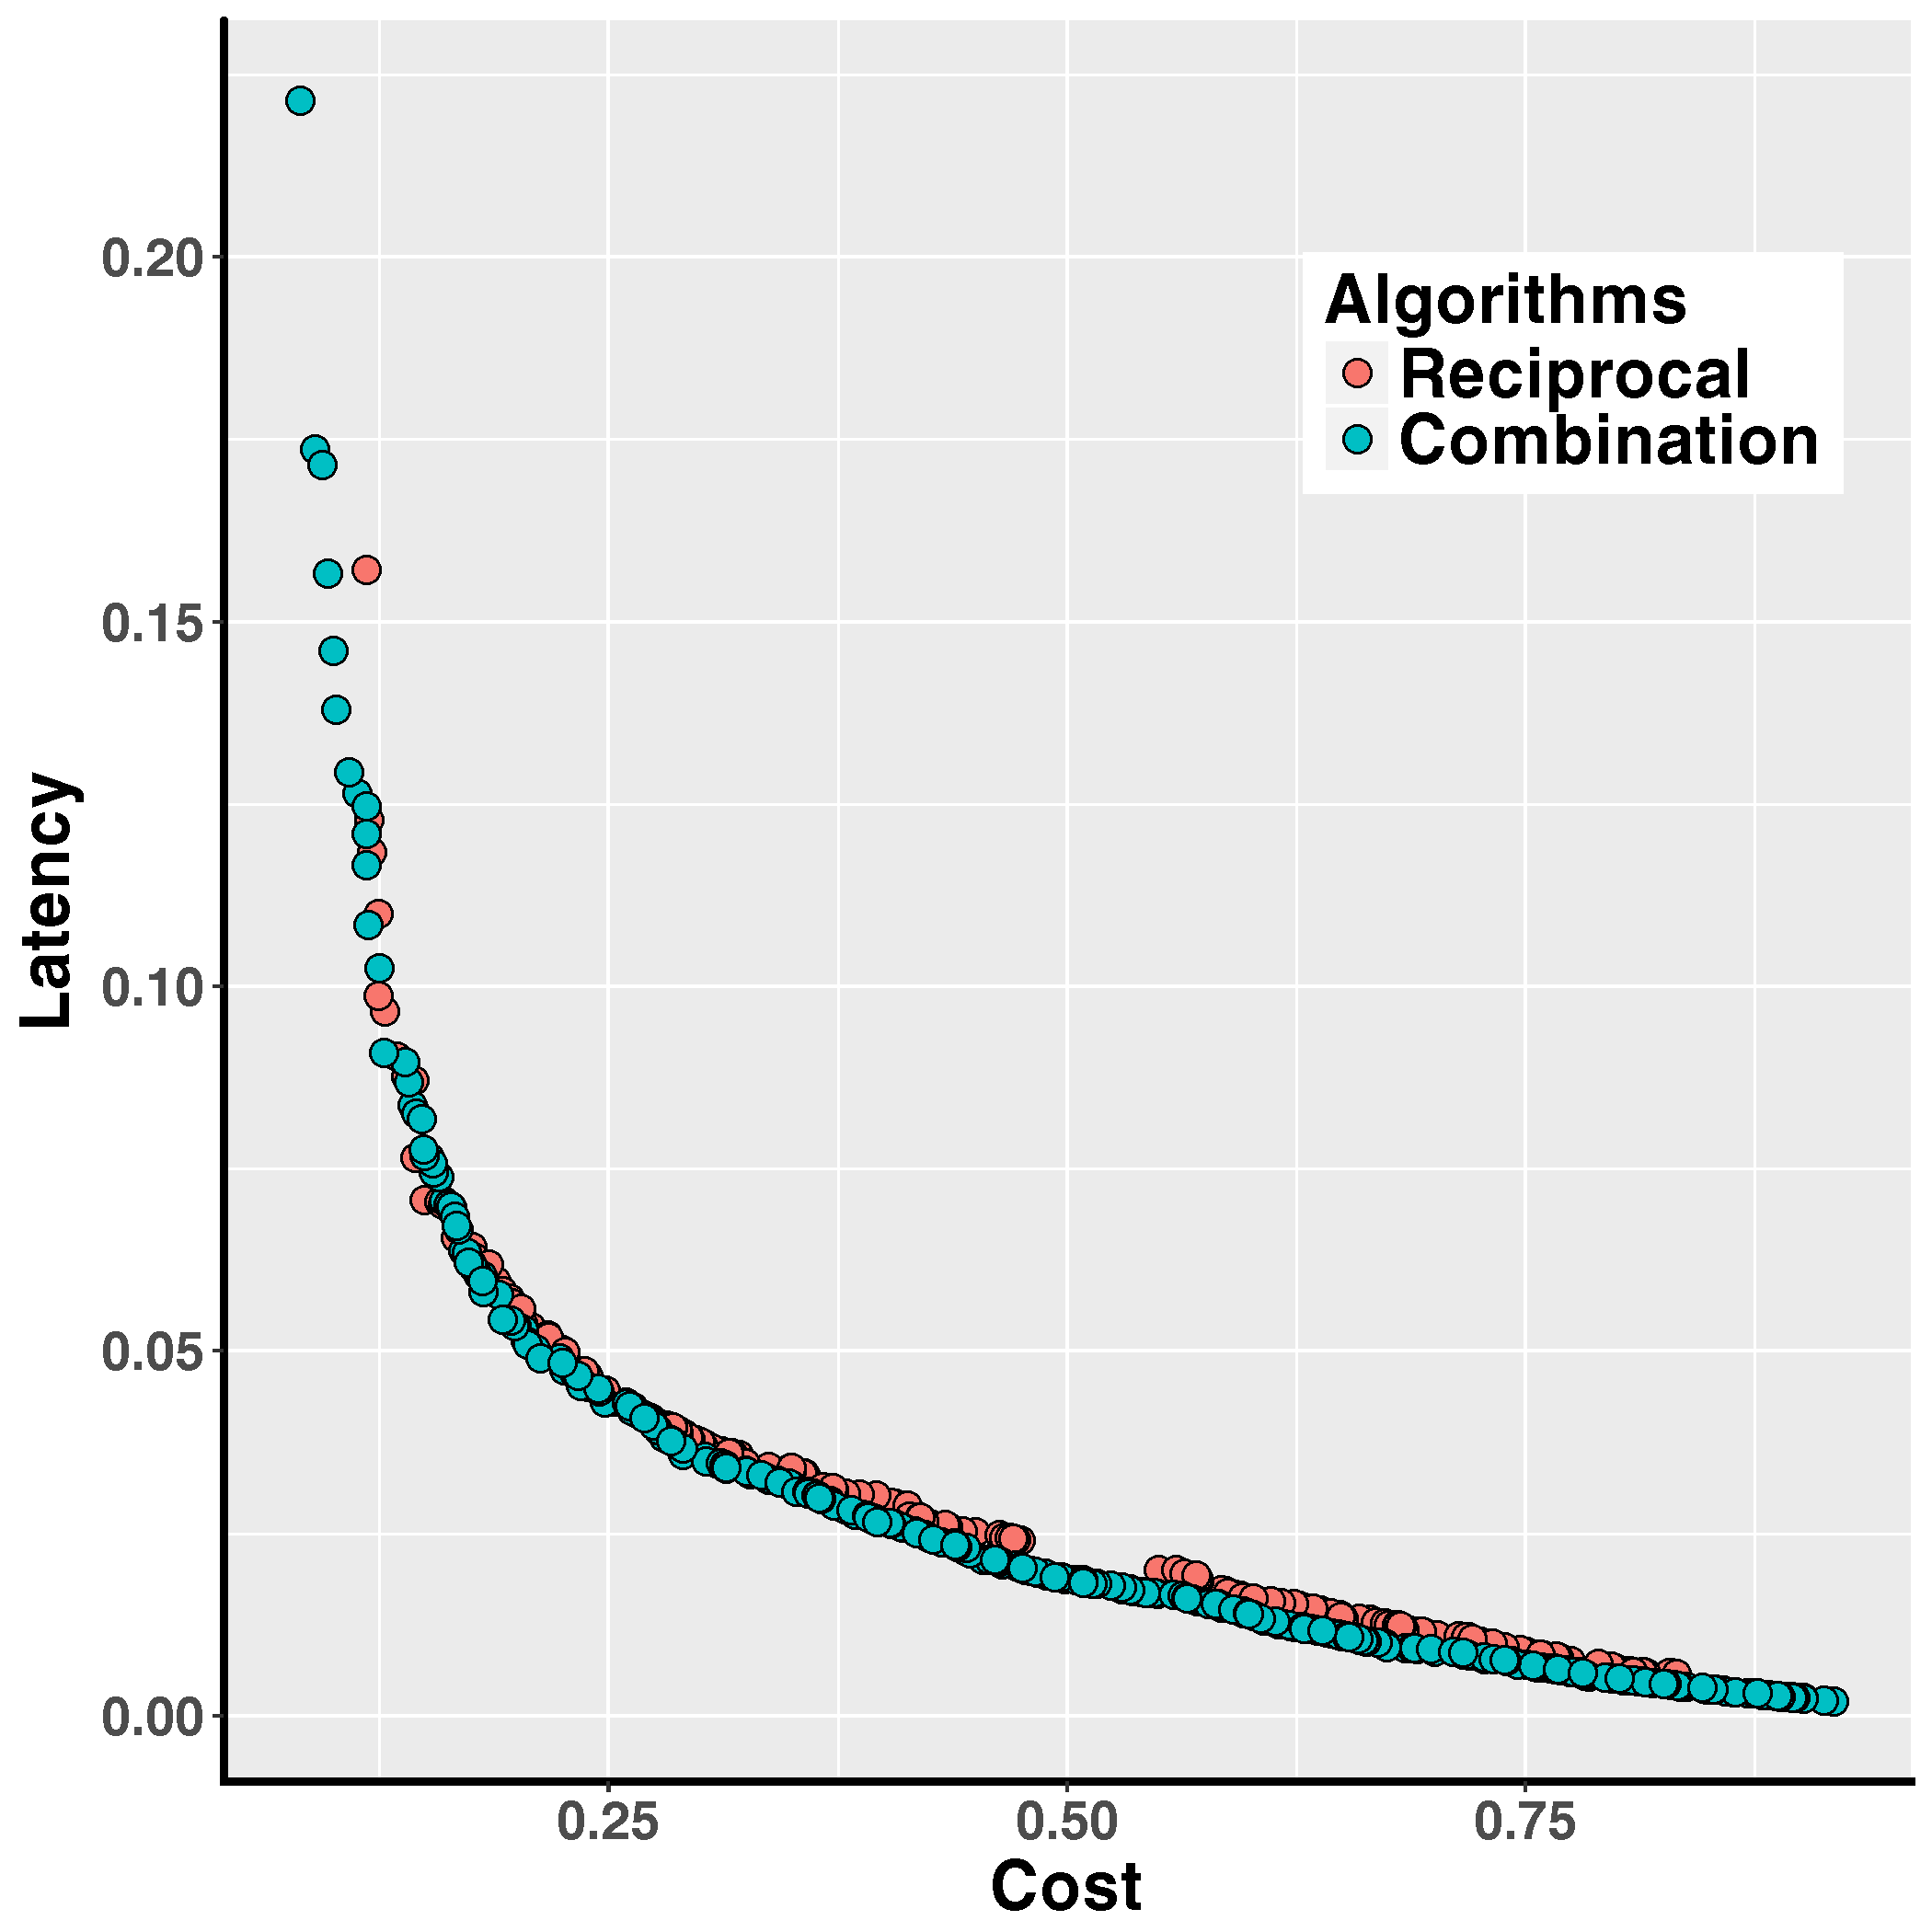
\includegraphics[width=\textwidth]{pics/combination_problem4.png}
    \caption{instance 4}
   \end{subfigure}
   \begin{subfigure}{0.49\linewidth}
       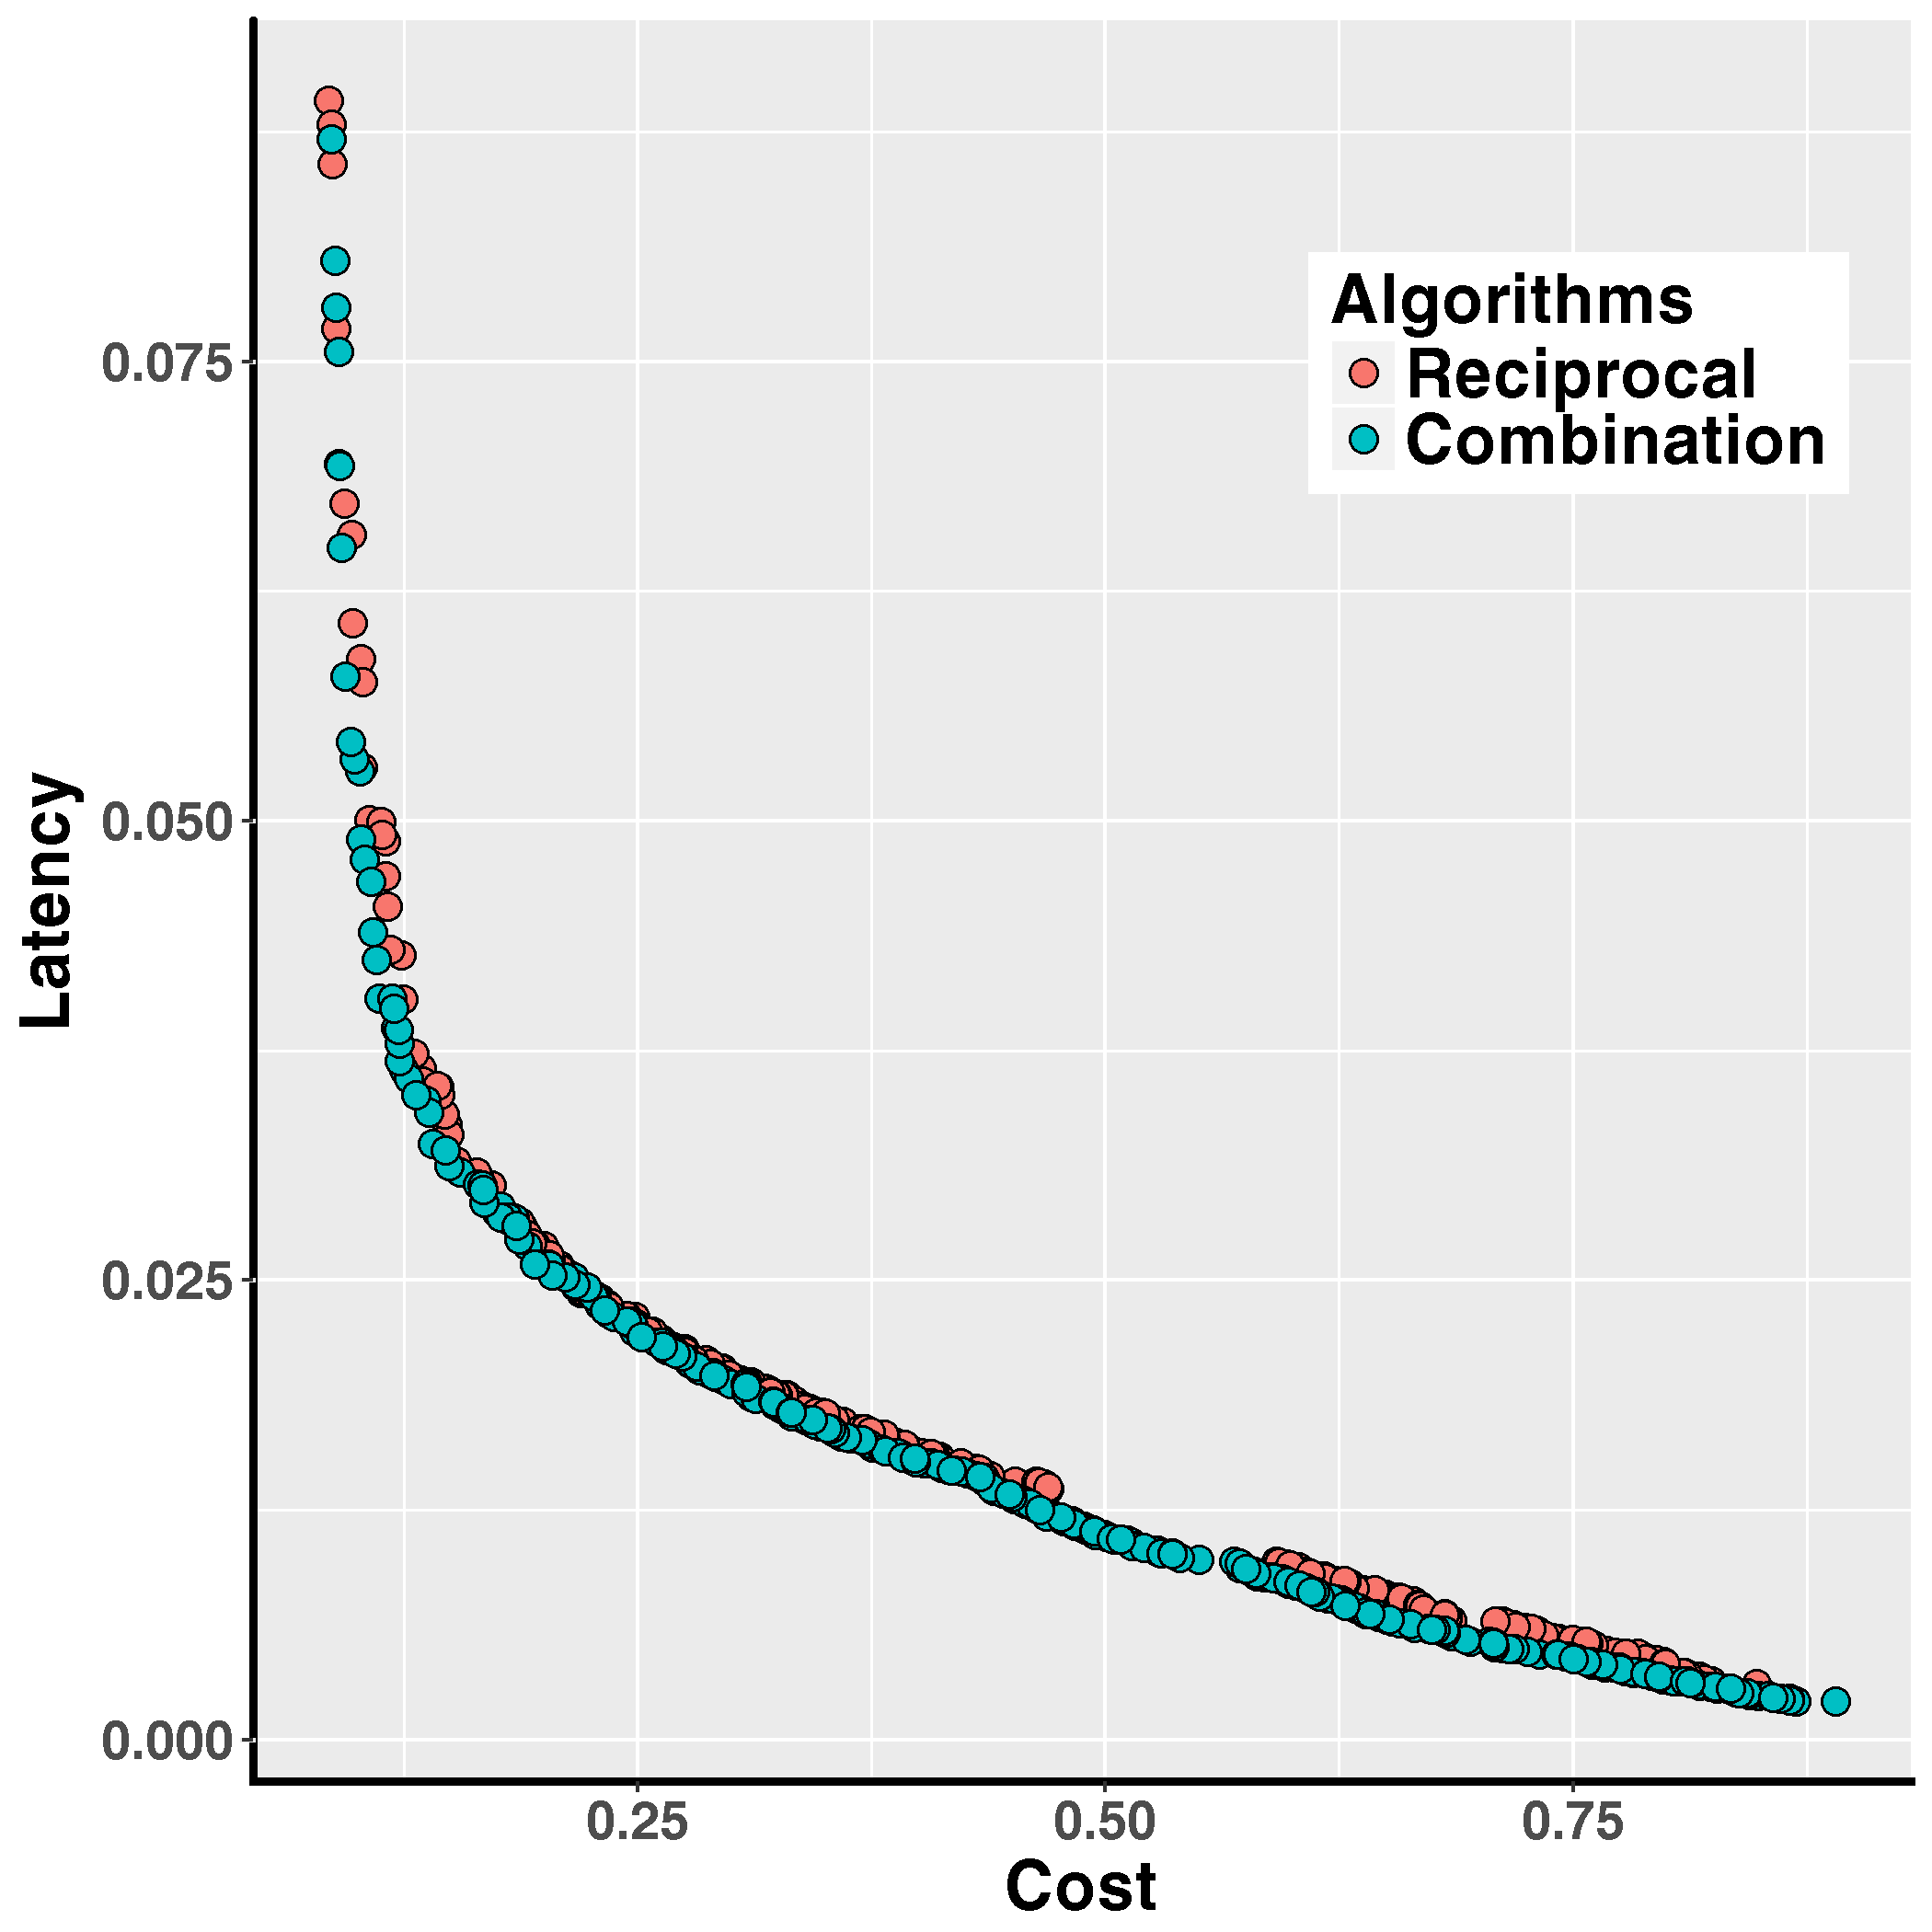
\includegraphics[width=\textwidth]{pics/combination_problem5.png}
    \caption{instance 5}
   \end{subfigure}
   \caption{Combination of Static Function Experiments:  The non-dominated solutions among
the sets obtained by 40 independent runs of combination of static thresholds and the Reciprocal function}
   \label{fig:combination}
\end{figure}

\vspace{-3 mm}
\subsection{BMOPSOCD versus BNSPSO, NSGA-II, and BPSO}

To evaluate the performance of our proposed BMOPSOCD with dynamic function, we conducted experiments to compare its performance with
BNSPSO, BPSO from our previous research \cite{Tan2016a}, and NSGA-II from \cite{Tan2016}. Based on the analysis in Section \ref{sec:expRound}, we use the Quadratic function as the rounding function. The results are shown in Table \ref{tab:results} and in Figure \ref{fig:total}. The figures show that our proposed BMOPSOCD dominate other algorithms in IGD (the small the better) and dominate other algorithms in HV (the bigger the better) except the instance 1. The margin between BMOPSOCD and other algorithms are huge. We can also observe a decline trend in the performance of other algorithms in HV. But the performance of BMOPSOCD maintains well in large test instances.
The only exception is instance 1, BPSO has the best HV value. On all instances, the $p$ value between BMOPSOCD is less than $10^{-10}$ which means BMOPSOCD is significantly better. In addition, only BMOPSOCD shows an excellent performance in terms of HV, when the number of variables increases. On all instances, BMOPSOCD achieved a considerably better performance than other three algorithms in IGD, due to the better coverage.

In comparison with BNSPSO and NSGA-II, BMOPSOCD with dynamic rounding function achieved significantly better convergence and diversity. One reason is that with the dynamic
rounding function, BMOPSOCD could move out of local optima. 
% In contrast, NSGA-II and BNSPSO are easy to be stuck at local optima. 
Other reason is the BMOPSOCD
keeps an external archive. Although the three algorithms maintain the same population, they produce different sizes of solutions. BMOPSOCD outputs an archive with a size of 250 while other two algorithms output a population of size 50.

In instance 1, the convergence of BMOPSOCD is worse than that of BPSO. 
% One reason is that BPSO runs 50 generations with the same weight for both objectives, it has more time to search alone the same direction. On the other hand, with dynamic rounding function, MOSPCOD might not completely converge. 
One reason is related to the problem size. BPSO has better performance in small problems. When the problem size increases, its performance drops rapidly. In contrast, BMOPSOCD with the dynamic rounding function is not much affected by the number of variables.

% \begin{figure*}
% \centering
%   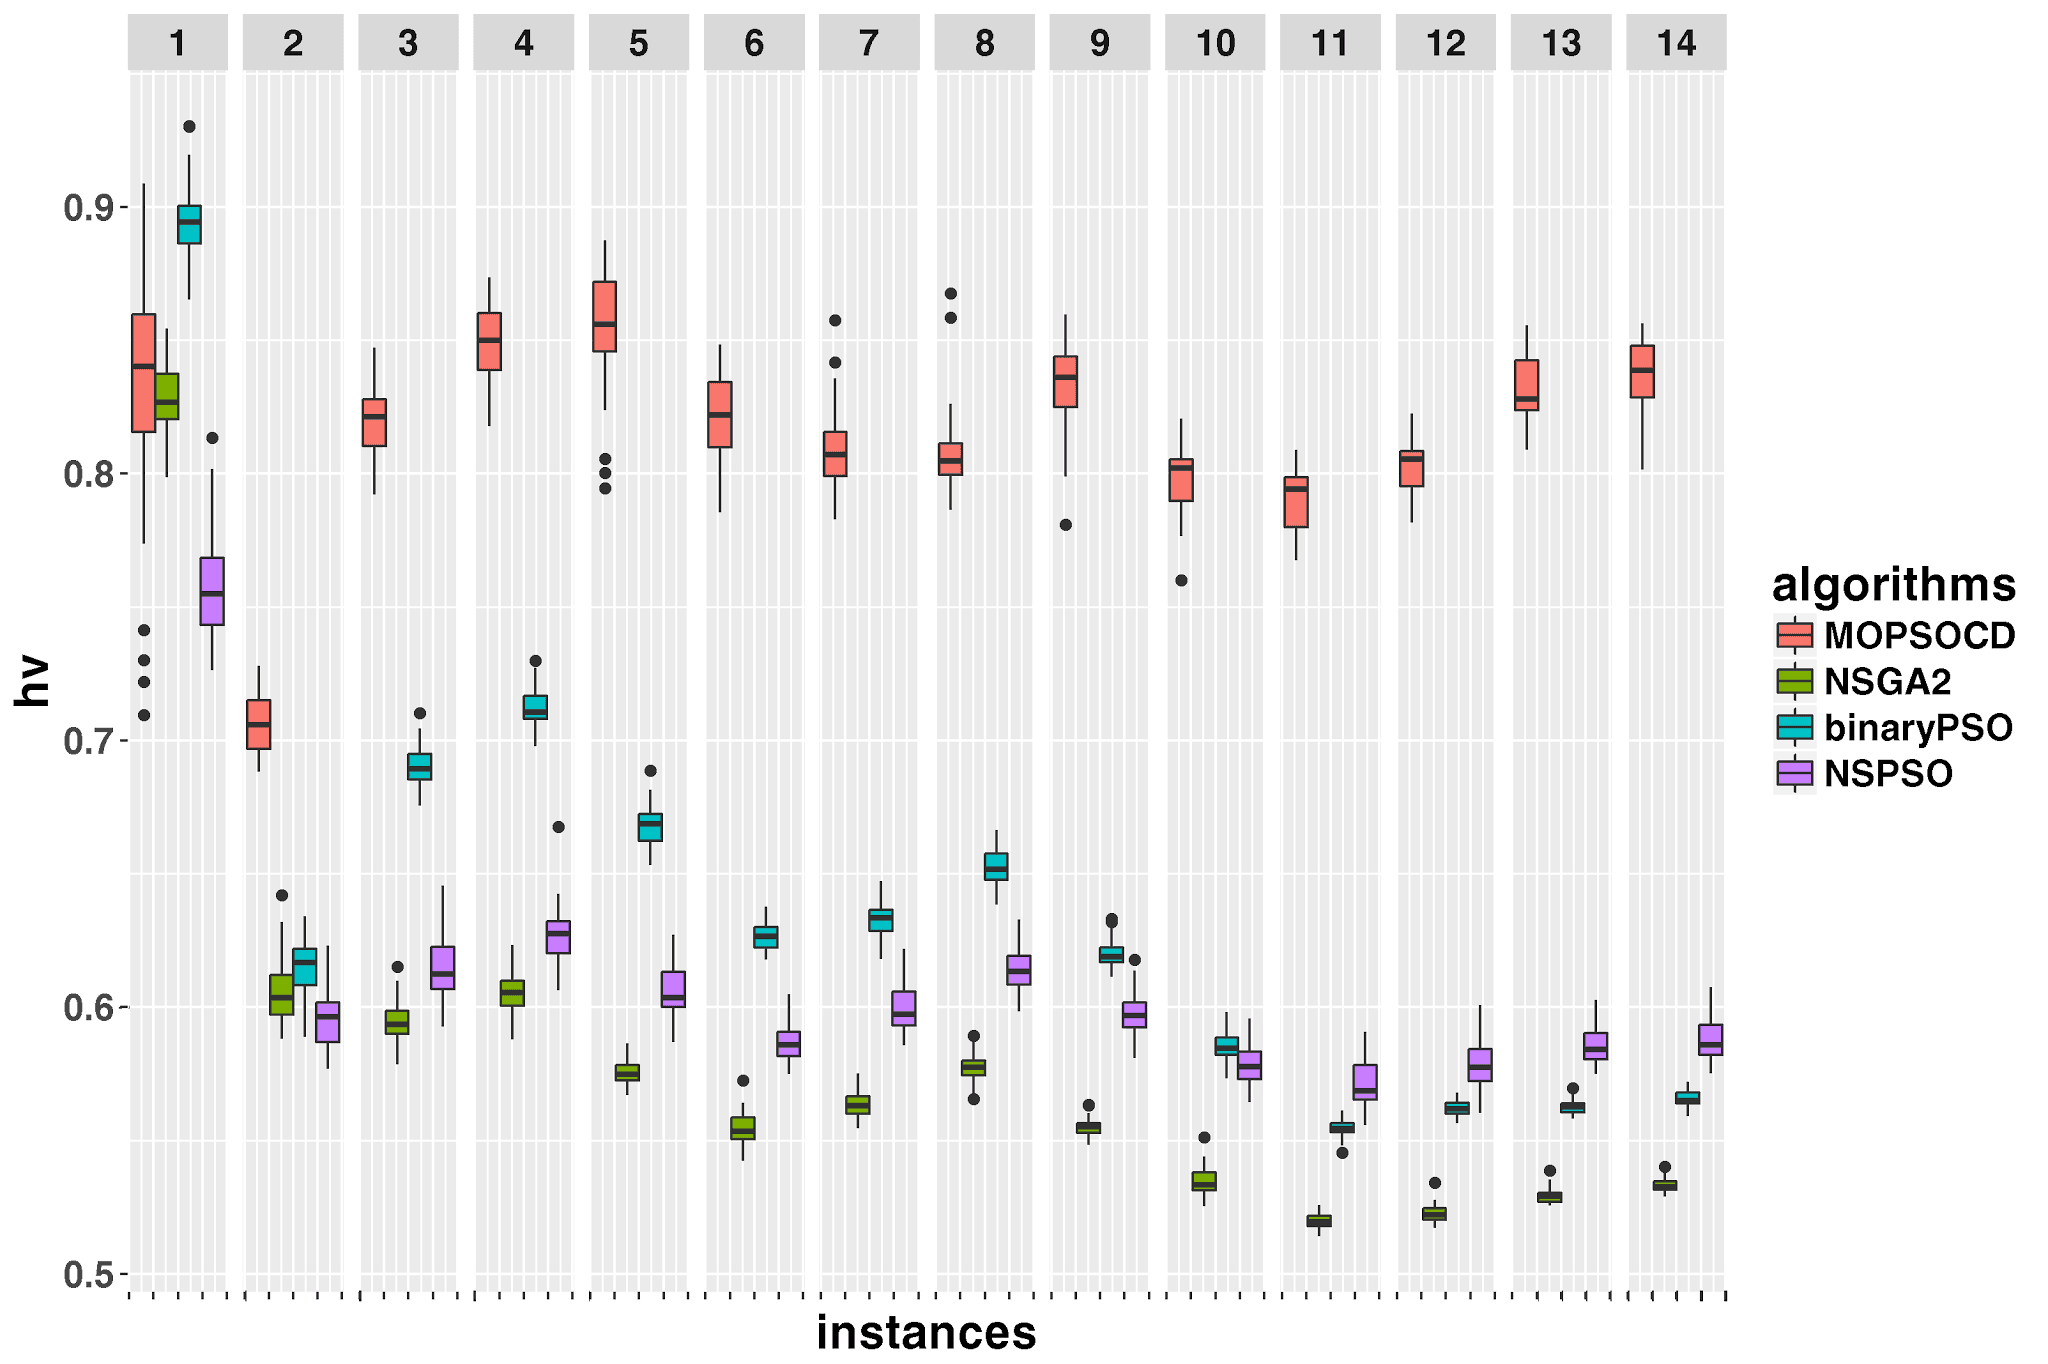
\includegraphics[width=0.7\textwidth]{pics/hv.png}
%   \caption{HyperVolume of BMOPSOCD, BNSPSO, NSGA-II and BPSO from 14 instances}
%   \label{fig:final_HyperVolume}
% \end{figure*}
% \begin{figure*}
% \centering
%   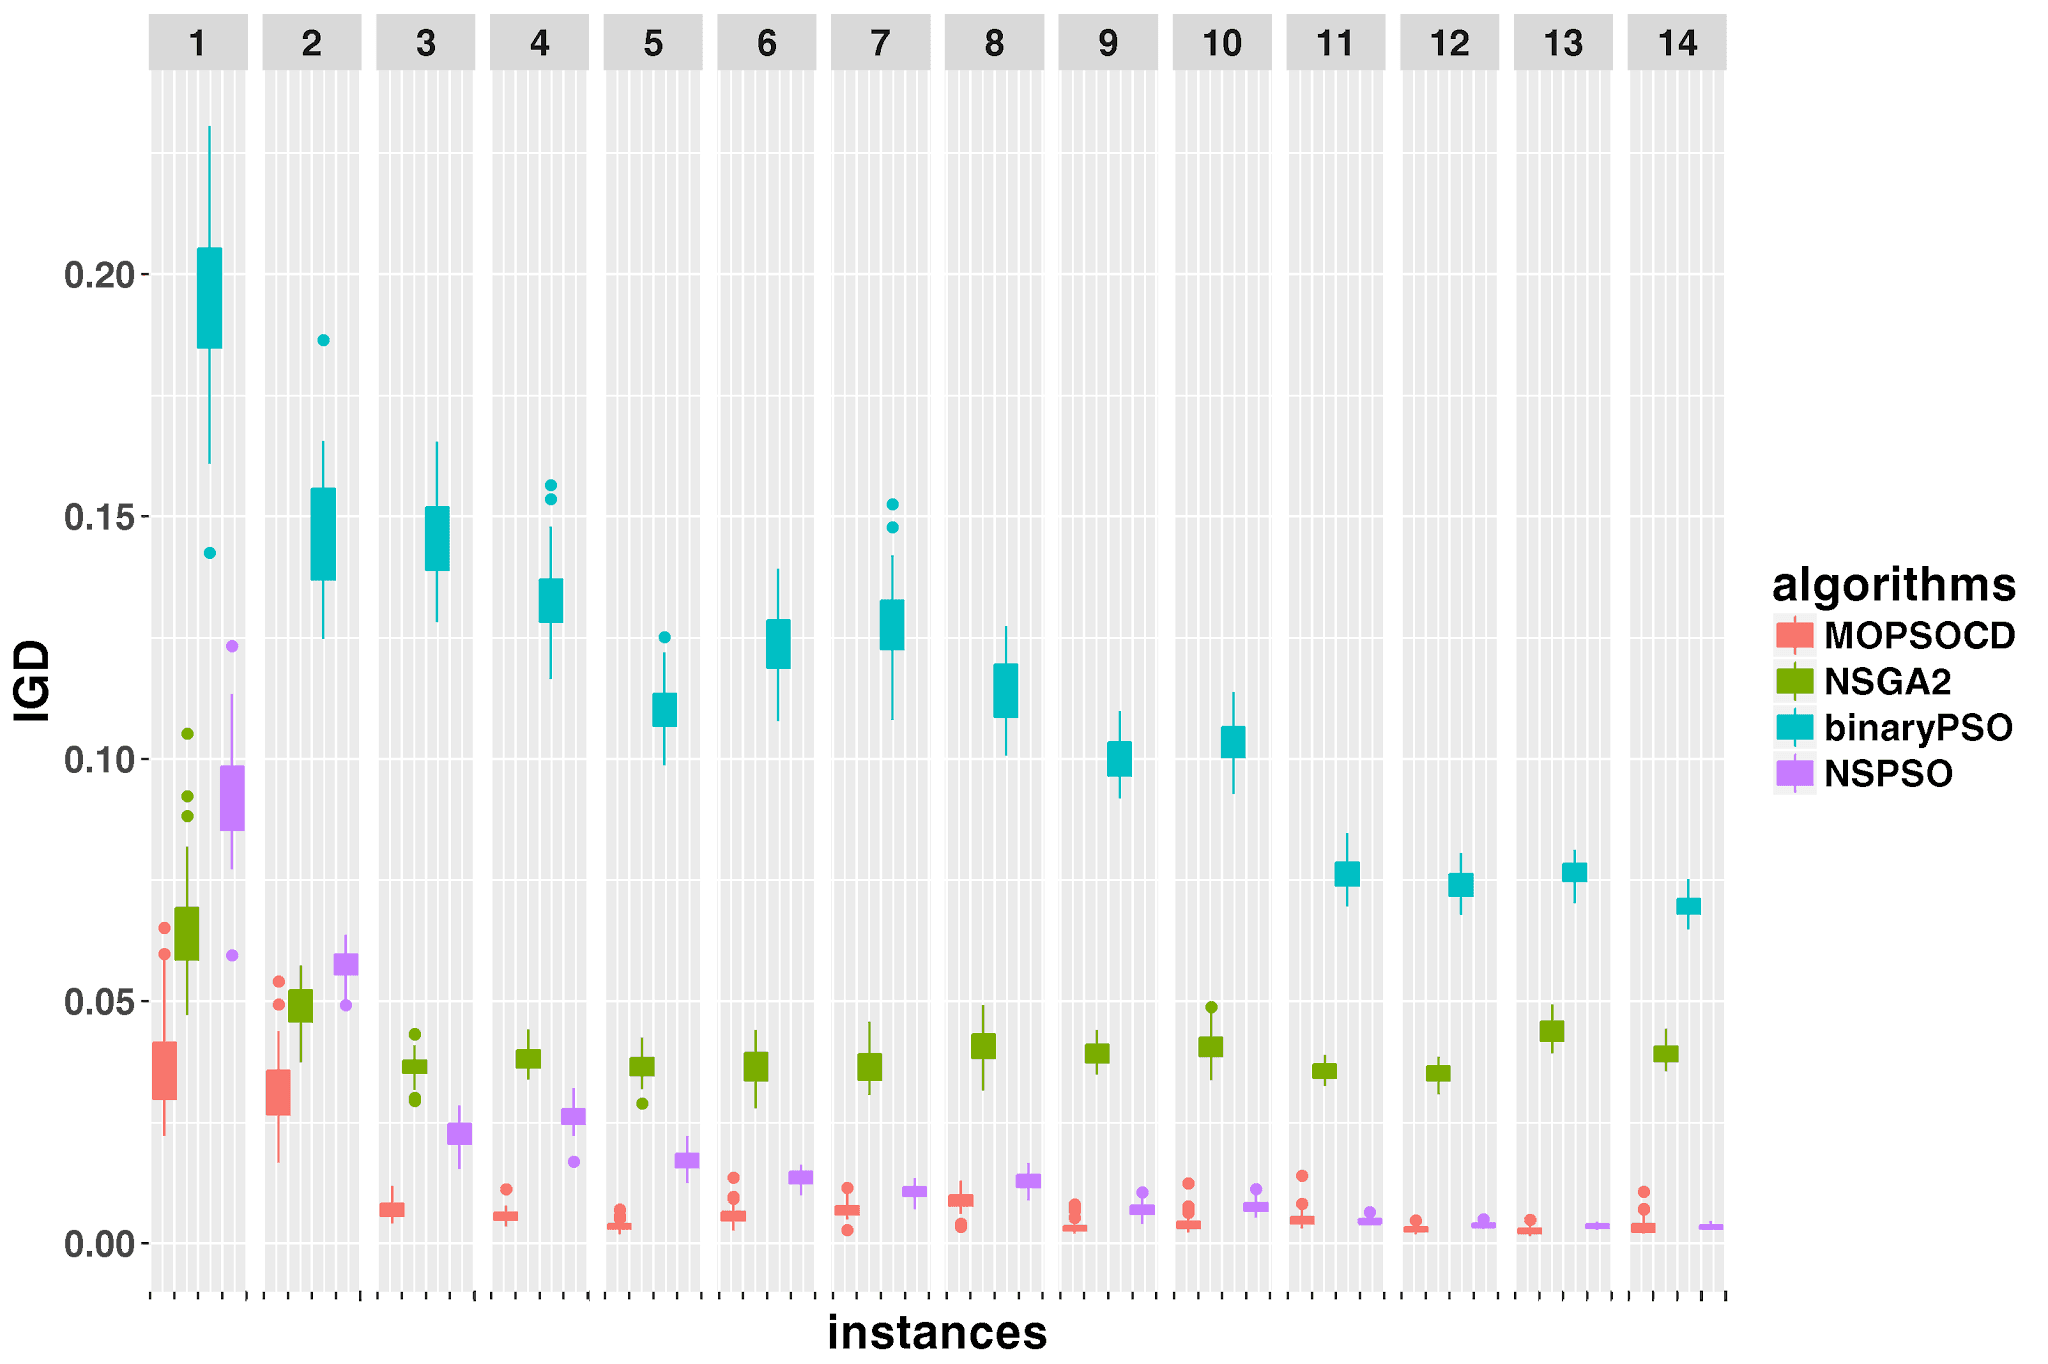
\includegraphics[width=0.7\textwidth]{pics/igd.png}
%   \caption{IGD of BMOPSOCD, BNSPSO, NSGA-II and BPSO from 14 instances}
%   \label{fig:final_igd}
% \end{figure*}

\begin{table*}[!htb]
\centering
\footnotesize



\scalebox{0.8}{
\begin{subtable}{.5\textwidth}
\centering
\begin{tabular}{|c|l|c|c|}
\hline
instances                         & \multicolumn{1}{c|}{Method}                                              & HV (avg $\pm$ sd)                                                                                                     & \multicolumn{1}{l|}{IGD (avg $\pm$ sd)}                                                                                                    \\ \hline
instance 1                       & \begin{tabular}[c]{@{}l@{}}BMOPSOCD\\ BNSPSO\\ NSGA-II\\ BPSO\end{tabular} & \begin{tabular}[c]{@{}c@{}}0.90 $\pm$ 0.04\\ 0.82 $\pm$ 0.018\\ 0.86 $\pm$ 0.013\\ \textbf{0.95 $\pm$ 0.015} \end{tabular}  & \begin{tabular}[c]{@{}c@{}}\textbf{3.73E-02 $\pm$ 1.03E-02} \\ 0.16 $\pm$ 3.45E-02\\  0.19 $\pm$ 3.21E-02\\ 0.46 $\pm$ 2.45E-02\end{tabular} \\ \hline
instance 2                       & \begin{tabular}[c]{@{}l@{}}BMOPSOCD\\ BNSPSO\\ NSGA-II\\ BPSO\end{tabular} & \begin{tabular}[c]{@{}c@{}}\textbf{0.77 $\pm$ 0.011} \\ 0.64 $\pm$ 0.001\\ 0.65 $\pm$ 0.011\\  0.65 $\pm$ 0.001\end{tabular} & \begin{tabular}[c]{@{}c@{}}\textbf{3.15E-02 $\pm$ 7.92E-03} \\ 0.15 $\pm$ 1.46E-02\\ 0.19 $\pm$ 1.81E-02\\  0.42 $\pm$ 1.54E-02\end{tabular} \\ \hline
instance 3                       & \begin{tabular}[c]{@{}l@{}}BMOPSOCD\\ BNSPSO\\ NSGA-II\\ BPSO\end{tabular} & \begin{tabular}[c]{@{}c@{}}\textbf{0.84 $\pm$ 0.012} \\ 0.64 $\pm$ 0.011\\ 0.61 $\pm$ 0.008\\ 0.71 $\pm$ 0.007\end{tabular}  & \begin{tabular}[c]{@{}c@{}}\textbf{7.03E-03 $\pm$ 1.92E-03} \\ 0.10 $\pm$ 6.35E-03\\ 0.16 $\pm$ 7.25E-03\\  0.30 $\pm$ 8.94E-03\end{tabular} \\ \hline
instance 4                       & \begin{tabular}[c]{@{}l@{}}BMOPSOCD\\ BNSPSO\\ NSGA-II\\ BPSO\end{tabular} & \begin{tabular}[c]{@{}c@{}}\textbf{0.86 $\pm$ 0.016} \\ 0.67 $\pm$ 0.012\\ 0.63 $\pm$ 0.008\\ 0.74 $\pm$ 0.008\end{tabular}  & \begin{tabular}[c]{@{}c@{}}\textbf{5.80E-03 $\pm$ 1.37E-03} \\ 0.11 $\pm$ 8.55E-03\\ 0.17 $\pm$ 9.11E-03 \\ 0.30 $\pm$ 8.62E-03\end{tabular} \\ \hline
instance 5                       & \begin{tabular}[c]{@{}l@{}}BMOPSOCD\\ BNSPSO\\ NSGA-II\\ BPSO\end{tabular} & \begin{tabular}[c]{@{}c@{}}\textbf{0.87 $\pm$ 0.014} \\ 0.63 $\pm$ 0.009\\ 0.59 $\pm$ 0.005\\ 0.69 $\pm$ 0.007\end{tabular}  & \begin{tabular}[c]{@{}c@{}}\textbf{3.74E-03 $\pm$ 1.02E-03} \\ 0.11 $\pm$ 7.93E-03\\ 0.17 $\pm$ 6.89E-03\\  0.24 $\pm$ 5.02E-03\end{tabular} \\ \hline
\multicolumn{1}{|l|}{instance 6} & \begin{tabular}[c]{@{}l@{}}BMOPSOCD\\ BNSPSO\\ NSGA-II\\ BPSO\end{tabular} & \begin{tabular}[c]{@{}c@{}}\textbf{0.84 $\pm$ 0.014} \\ 0.60 $\pm$ 0.007\\ 0.57 $\pm$ 0.006\\ 0.64 $\pm$ 0.005\end{tabular}  & \begin{tabular}[c]{@{}c@{}}\textbf{5.81E-03 $\pm$ 1.95E-03} \\ 0.11 $\pm$ 5.06E-03\\ 0.18 $\pm$ 8.01E-03 \\ 0.28 $\pm$ 5.88E-03\end{tabular} \\ \hline
instance 7                       & \begin{tabular}[c]{@{}l@{}}BMOPSOCD\\ BNSPSO\\ NSGA-II\\ BPSO\end{tabular} & \begin{tabular}[c]{@{}c@{}}\textbf{0.86 $\pm$ 0.015} \\ 0.62 $\pm$ 0.008\\ 0.57 $\pm$ 0.005\\ 0.65 $\pm$ 0.006\end{tabular}  & \begin{tabular}[c]{@{}c@{}}\textbf{7.13E-03 $\pm$ 1.70E-03} \\ 0.10 $\pm$ 4.58E-03\\ 0.17 $\pm$ 6.48E-03 \\ 0.27 $\pm$ 7.92E-03\end{tabular} \\ \hline
\end{tabular}
\end{subtable}

\begin{subtable}{.5\textwidth}
\centering
\begin{tabular}{|c|l|c|c|}
\hline
instances                         & \multicolumn{1}{c|}{Method}                                              & HV (avg $\pm$ sd)                                                                                                     & \multicolumn{1}{l|}{IGD (avg $\pm$ sd)}                                                                                                    \\ \hline
instance 8                       & \begin{tabular}[c]{@{}l@{}}BMOPSOCD\\ BNSPSO\\ NSGA-II\\ BPSO\end{tabular} & \begin{tabular}[c]{@{}c@{}}\textbf{0.87 $\pm$ 0.015} \\ 0.63 $\pm$ 0.008\\ 0.59 $\pm$ 0.005\\ 0.67 $\pm$ 0.007\end{tabular}  & \begin{tabular}[c]{@{}c@{}}\textbf{8.77E-03 $\pm$ 1.90E-03} \\ 0.12 $\pm$ 5.81E-03\\ 0.19 $\pm$ 6.17E-03 \\ 0.27 $\pm$ 5.86E-03\end{tabular} \\ \hline
instance 9                       & \begin{tabular}[c]{@{}l@{}}BMOPSOCD\\ BNSPSO\\ NSGA-II\\ BPSO\end{tabular} & \begin{tabular}[c]{@{}c@{}}\textbf{0.86 $\pm$ 0.016} \\ 0.62 $\pm$ 0.009\\ 0.56 $\pm$ 0.004\\ 0.63 $\pm$ 0.005\end{tabular}  & \begin{tabular}[c]{@{}c@{}}\textbf{3.58E-03 $\pm$ 1.53E-03} \\ 0.11 $\pm$ 5.33E-03\\ 0.17 $\pm$ 3.56E-03 \\ 0.22 $\pm$ 3.22E-03\end{tabular} \\ \hline
instance 10                      & \begin{tabular}[c]{@{}l@{}}BMOPSOCD\\ BNSPSO\\ NSGA-II\\ BPSO\end{tabular} & \begin{tabular}[c]{@{}c@{}}\textbf{0.83 $\pm$ 0.012} \\ 0.60 $\pm$ 0.008\\ 0.55 $\pm$ 0.005\\ 0.6 $\pm$ 0.005\end{tabular}  & \begin{tabular}[c]{@{}c@{}}\textbf{4.30E-03 $\pm$ 1.75E-03} \\ 0.11 $\pm$ 4.97E-03\\ 0.19 $\pm$ 5.62E-03 \\ 0.25 $\pm$ 3.91E-03\end{tabular} \\ \hline
instance 11                      & \begin{tabular}[c]{@{}l@{}}BMOPSOCD\\ BNSPSO\\ NSGA-II\\ BPSO\end{tabular} & \begin{tabular}[c]{@{}c@{}}\textbf{0.82 $\pm$ 0.012} \\ 0.59 $\pm$ 0.009\\ 0.53 $\pm$ 0.003\\ 0.56 $\pm$ 0.003\end{tabular} & \begin{tabular}[c]{@{}c@{}}\textbf{5.19E-03 $\pm$ 1.81E-03} \\ 0.12 $\pm$ 4.22E-03\\ 0.20 $\pm$ 2.74E-03 \\ 0.24 $\pm$ 3.36E-03\end{tabular} \\ \hline
instance 12                      & \begin{tabular}[c]{@{}l@{}}BMOPSOCD\\ BNSPSO\\ NSGA-II\\ BPSO\end{tabular} & \begin{tabular}[c]{@{}c@{}}\textbf{0.82 $\pm$ 0.01} \\ 0.60 $\pm$ 0.009\\ 0.53 $\pm$ 0.003\\ 0.57 $\pm$ 0.003\end{tabular} & \begin{tabular}[c]{@{}c@{}}\textbf{3.12E-03 $\pm$ 6.71E-04} \\ 0.12 $\pm$ 4.15E-03\\ 0.20 $\pm$ 3.08E-03 \\ 0.24 $\pm$ 2.50E-03\end{tabular} \\ \hline
instance 13                      & \begin{tabular}[c]{@{}l@{}}BMOPSOCD\\ BNSPSO\\ NSGA-II\\ BPSO\end{tabular} & \begin{tabular}[c]{@{}c@{}}\textbf{0.86 $\pm$ 0.012} \\ 0.60 $\pm$ 0.008\\ 0.54 $\pm$ 0.003\\ 0.57 $\pm$ 0.004\end{tabular} & \begin{tabular}[c]{@{}c@{}}\textbf{2.63E-03 $\pm$ 6.73E-04} \\ 0.12 $\pm$ 3.46E-03\\ 0.20 $\pm$ 3.04E-03 \\ 0.22 $\pm$ 2.01E-03\end{tabular} \\ \hline
instance 14                      & \begin{tabular}[c]{@{}l@{}}BMOPSOCD\\ BNSPSO\\ NSGA-II\\ BPSO\end{tabular} & \begin{tabular}[c]{@{}c@{}}\textbf{0.86 $\pm$ 0.015} \\ 0.61 $\pm$ 0.009\\ 0.54 $\pm$ 0.002\\ 0.57 $\pm$ 0.003\end{tabular} & \begin{tabular}[c]{@{}c@{}}\textbf{3.66E-03 $\pm$ 1.75E-03} \\ 0.13 $\pm$ 3.85E-03\\ 0.22 $\pm$ 3.24E-03 \\ 0.25 $\pm$ 1.83E-03\end{tabular} \\ \hline
\end{tabular}
\end{subtable}

}
\caption{Comparison between BMOPSOCD, BNSPSO, NSGA-II and BPSO: The non-dominated solutions among the sets obtained by 40 independent runs of different algorithms}
\label{tab:results}
\end{table*}

Regarding execution time (Table \ref{tab:time}), BMOPSOCD has similar execution time with other approaches. It achieves the best or the second best performance for 11 out of 14 instances.
The reason is the velocity and position calculation (Equation \ref{eq:updatePosition} and \ref{eq:updateVelocity}) are linear so that these calculations can be vectorized. Conversely, for binary PSO, new positions are calculated by a sigmoid function which is non-linear. Therefore, an implementation of binary PSO must apply loop in the calculation.

% \begin{figure}
% \centering
%   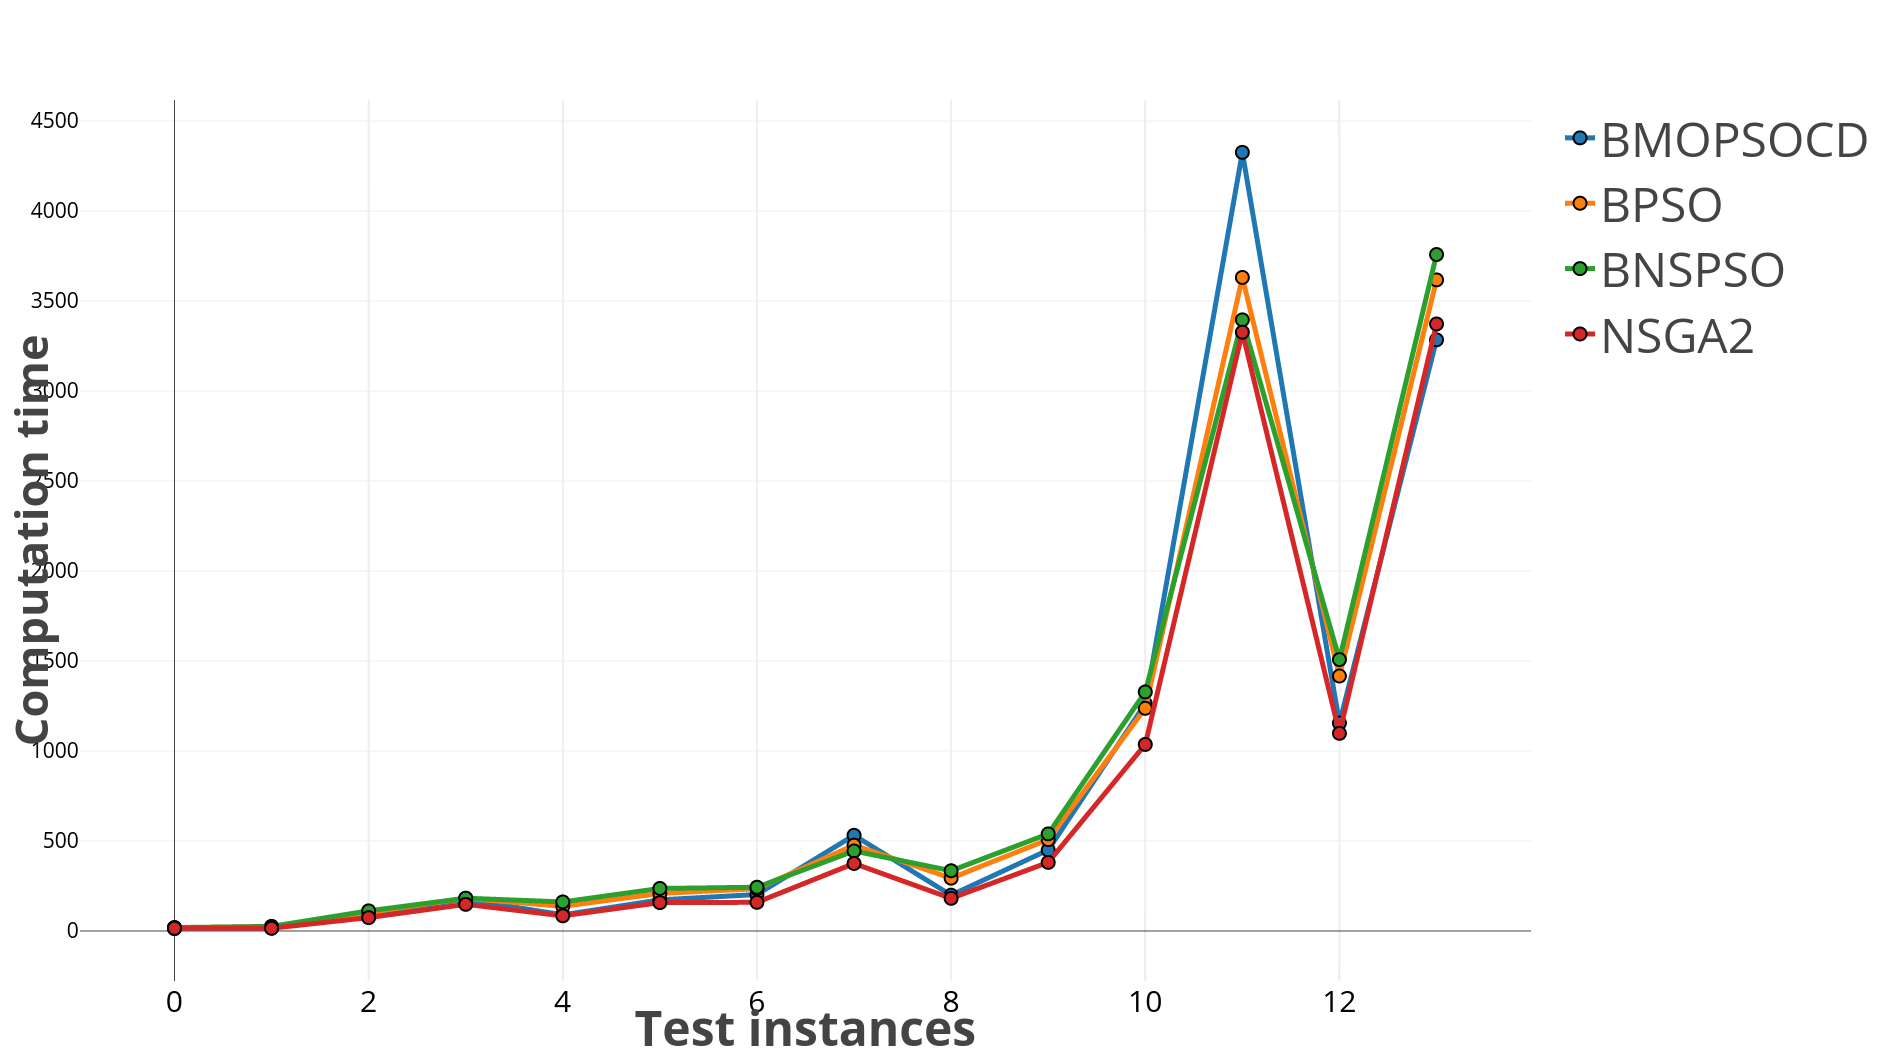
\includegraphics[width=0.45\textwidth]{pics/time.png}
%   \caption{Computation time of BMOPSOCD, BNSPSO, NSGA-II and BPSO from 14 instances}
%   \label{fig:final_time}
% \end{figure}


\begin{table*}[th]
\centering
\footnotesize
\scalebox{0.8}{

\begin{subtable}{.6\textwidth}
\centering
\begin{tabular}{lllll}
\hline
\multicolumn{1}{l|}{}           & BPSO            & BMOPSOCD         & BNSPSO          & NSGA-II         \\ \hline
\multicolumn{1}{l|}{instance 1} & 17.99 $\pm$  0.26 & \textbf{12.98 $\pm$ 0.18}   & 19.00 $\pm$ 0.17  & 15.35 $\pm$ 0.15  \\ 
\multicolumn{1}{l|}{instance 2} & 23.55 $\pm$ 0.27  & 16.18 $\pm$ 0.26   & 25.52 $\pm$ 0.27  & \textbf{15.38 $\pm$ 0.31}  \\
\multicolumn{1}{l|}{instance 3} & 103.65 $\pm$ 1.87 & 94.98 $\pm$ 7.28   & 111.86 $\pm$ 1.11 & \textbf{74.34 $\pm$ 0.61}  \\
\multicolumn{1}{l|}{instance 4} & 181.20 $\pm$ 4.40 & 175.99 $\pm$ 9.67  & 182.09 $\pm$ 1.86 & 147.98 $\pm$ 1.30 \\
\multicolumn{1}{l|}{instance 5} & 137.03 $\pm$ 0.87 & 89.74 $\pm$ 8.53   & 161.31 $\pm$ 0.95 & \textbf{84.17 $\pm$ 1.03}  \\
\multicolumn{1}{l|}{instance 6} & 208.63 $\pm$ 2.23 & 172.80 $\pm$ 7.68  & 236.23 $\pm$ 2.72 & \textbf{157.52 $\pm$ 1.62} \\
\multicolumn{1}{l|}{instance 7} & 234.73 $\pm$ 6.42 & 202.68 $\pm$ 10.46 & 242.94 $\pm$ 9.00 & \textbf{159.26 $\pm$ 1.31} \\
\hline
\end{tabular}
\end{subtable}

\begin{subtable}{.6\linewidth}
\centering
\begin{tabular}{lllll}
\hline
\multicolumn{1}{l|}{}            & BPSO              & BMOPSOCD           & BNSPSO             & NSGA-II           \\ \hline
\multicolumn{1}{l|}{instance 8}  & 476.76 $\pm$ 22.40  & 531.64 $\pm$ 43.14   & 444.41 $\pm$ 22.86   & \textbf{375.05 $\pm$ 4.11}   \\ 
\multicolumn{1}{l|}{instance 9}  & 293.43 $\pm$ 3.01   & 198.81 $\pm$ 7.11    & 334.62 $\pm$ 2.81    & \textbf{181.30 $\pm$ 3.06}   \\
\multicolumn{1}{l|}{instance 10} & 507.72 $\pm$ 4.19   & 449.91 $\pm$ 26.00   & 539.51 $\pm$ 4.06    & \textbf{381.18  $\pm$ 3.06}  \\
\multicolumn{1}{l|}{instance 11} & 1237.30 $\pm$ 42.06 & 1262.79 $\pm$ 91.65  & 1328.17 $\pm$ 12.67  & \textbf{1036.53 $\pm$ 35.38} \\
\multicolumn{1}{l|}{instance 12} & 3631.14 $\pm$ 17.70 & 4326.22 $\pm$ 478.14 & 3395.47 $\pm$ 100.51 & \textbf{3326.94 $\pm$ 38.21} \\
\multicolumn{1}{l|}{instance 13} & 1416.63 $\pm$ 26.60 & 1155.21 $\pm$ 28.85  & 1507.92 $\pm$ 25.74  & \textbf{1098.08 $\pm$ 17.36} \\
\multicolumn{1}{l|}{instance 14} & 3617.53 $\pm$ 34.13 & \textbf{3284.66 $\pm$ 124.13} & 3759.51 $\pm$ 61.49  & 3372.53 $\pm$ 31.05 \\
\hline
\end{tabular}
\end{subtable}
}
\caption{Execution time (average and standard deviation in seconds)}
\label{tab:time}
\end{table*}





\begin{figure*}[ht]
   \centering
   \begin{subfigure}{0.21\linewidth}
       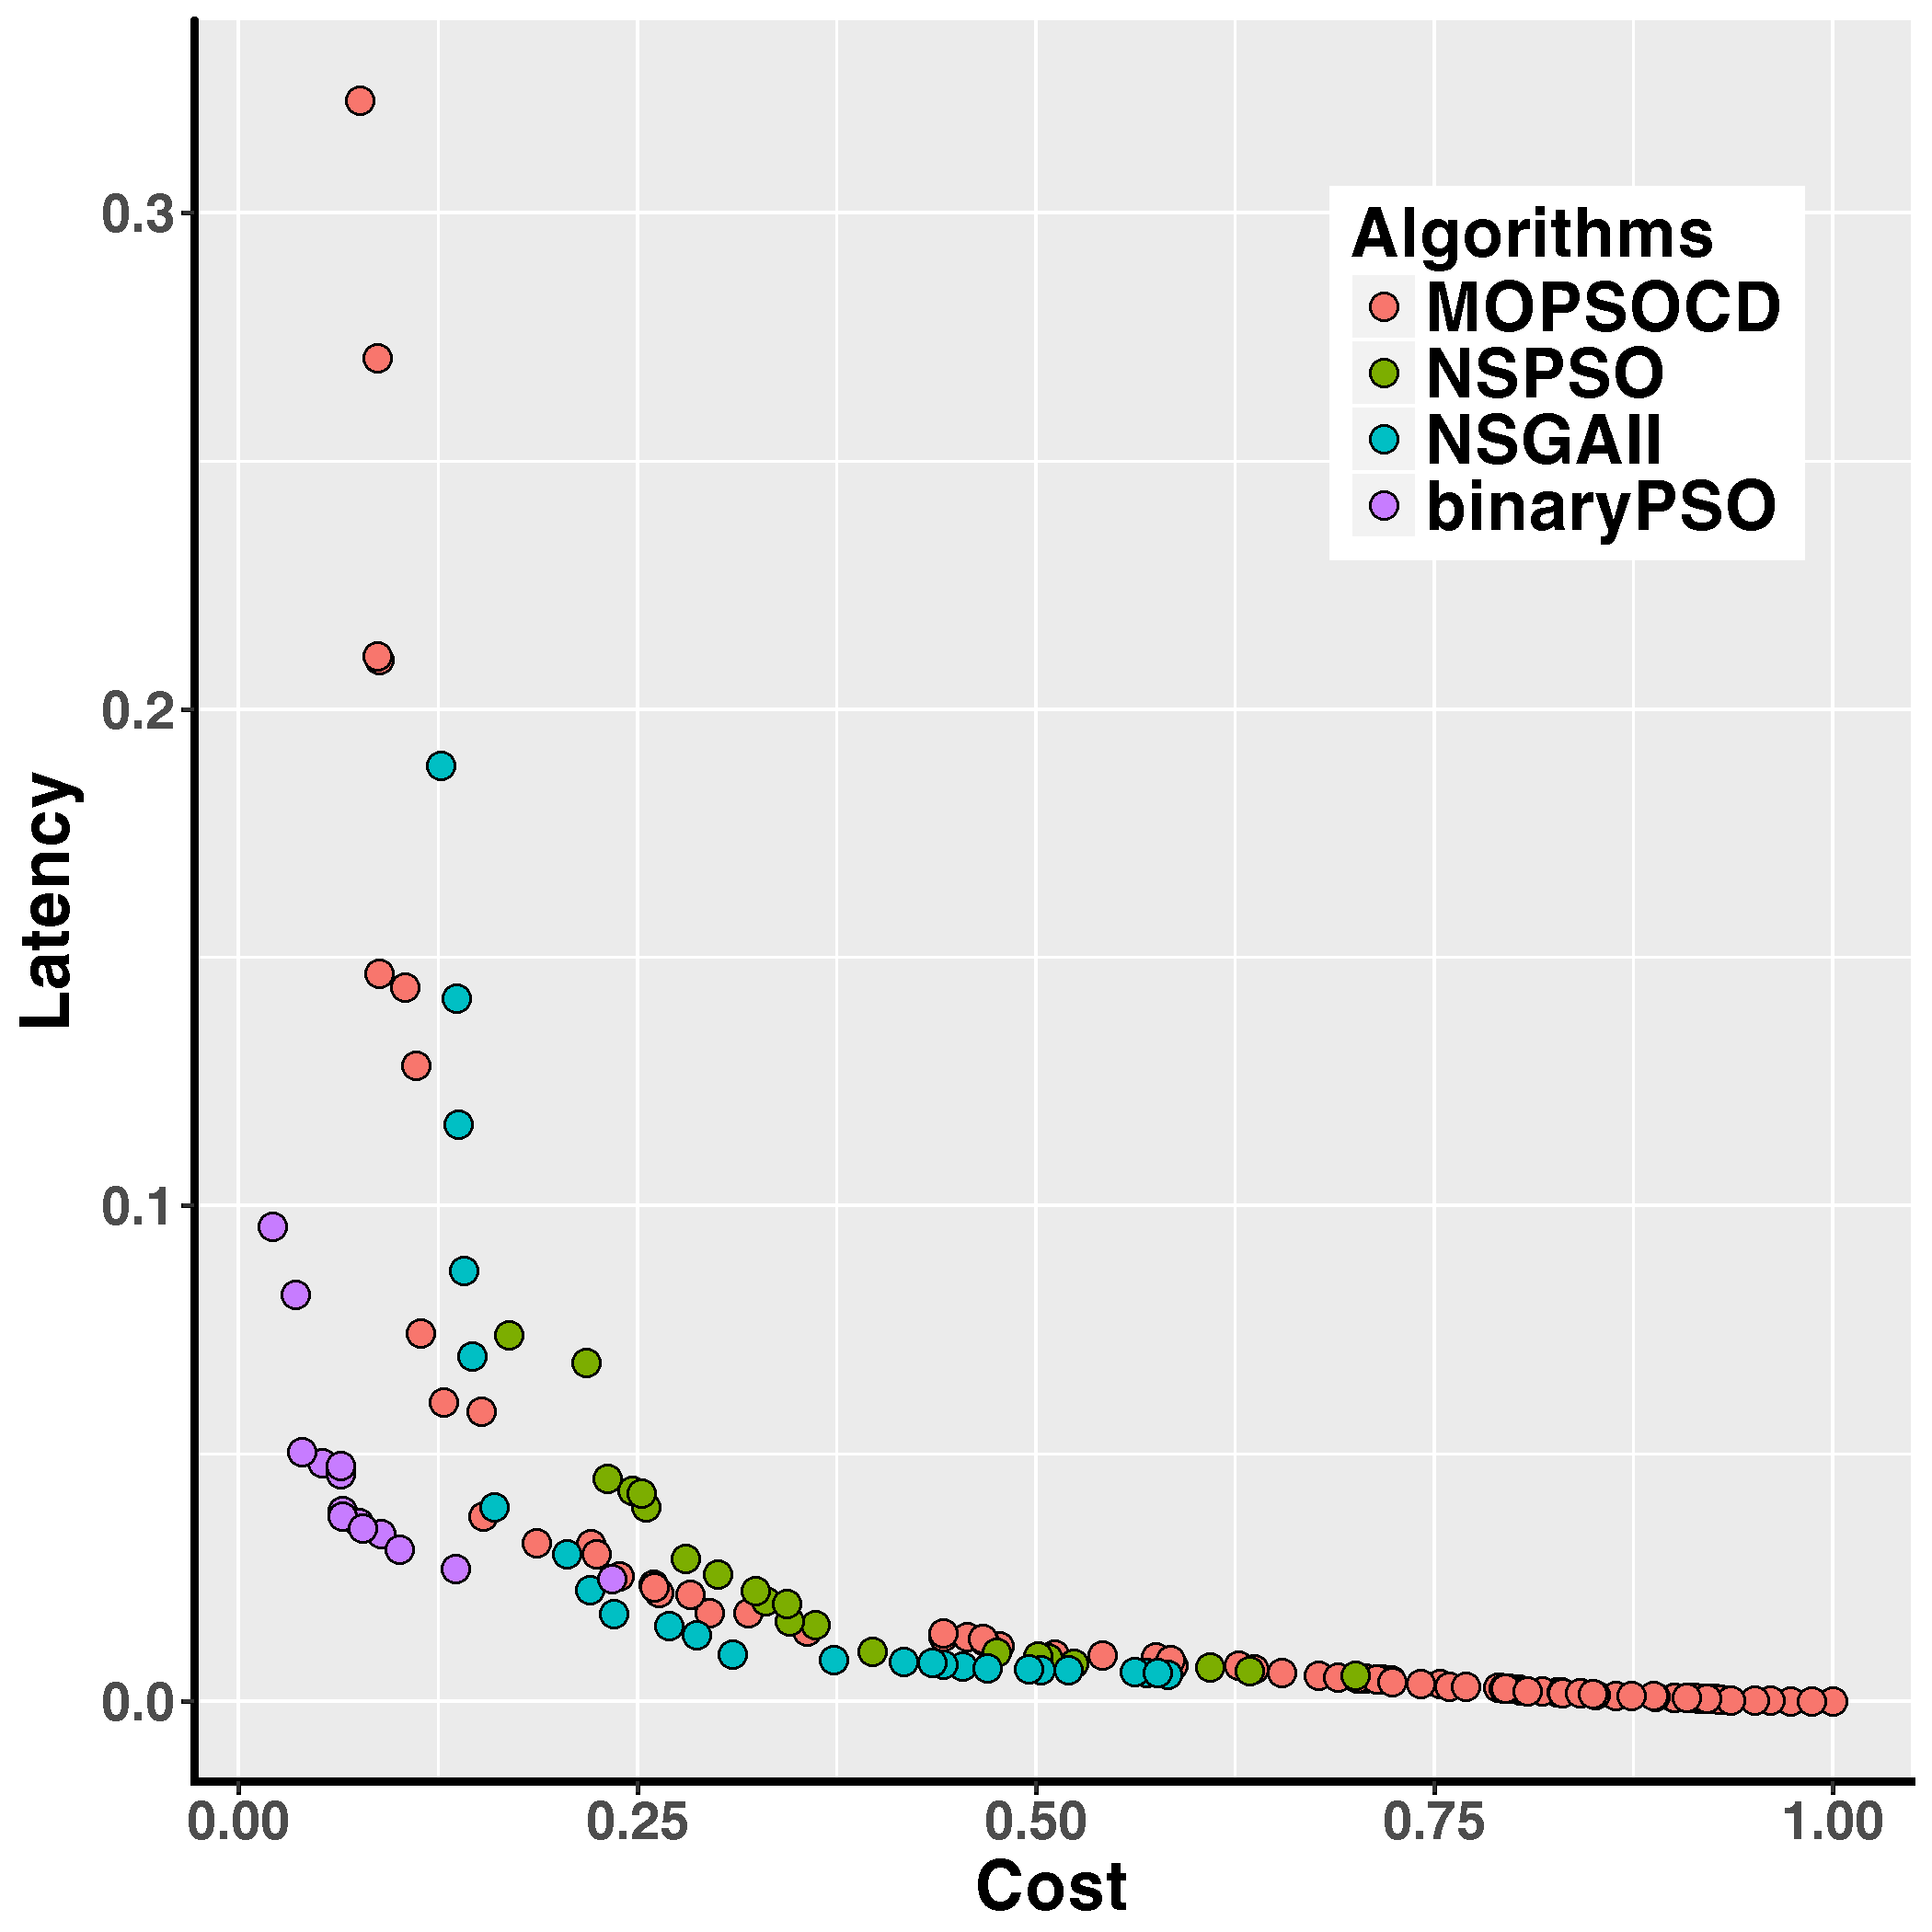
\includegraphics[width=\textwidth]{pics/total1.png}
    \caption{instance 1}
   \end{subfigure}
   \begin{subfigure}{0.21\linewidth}
       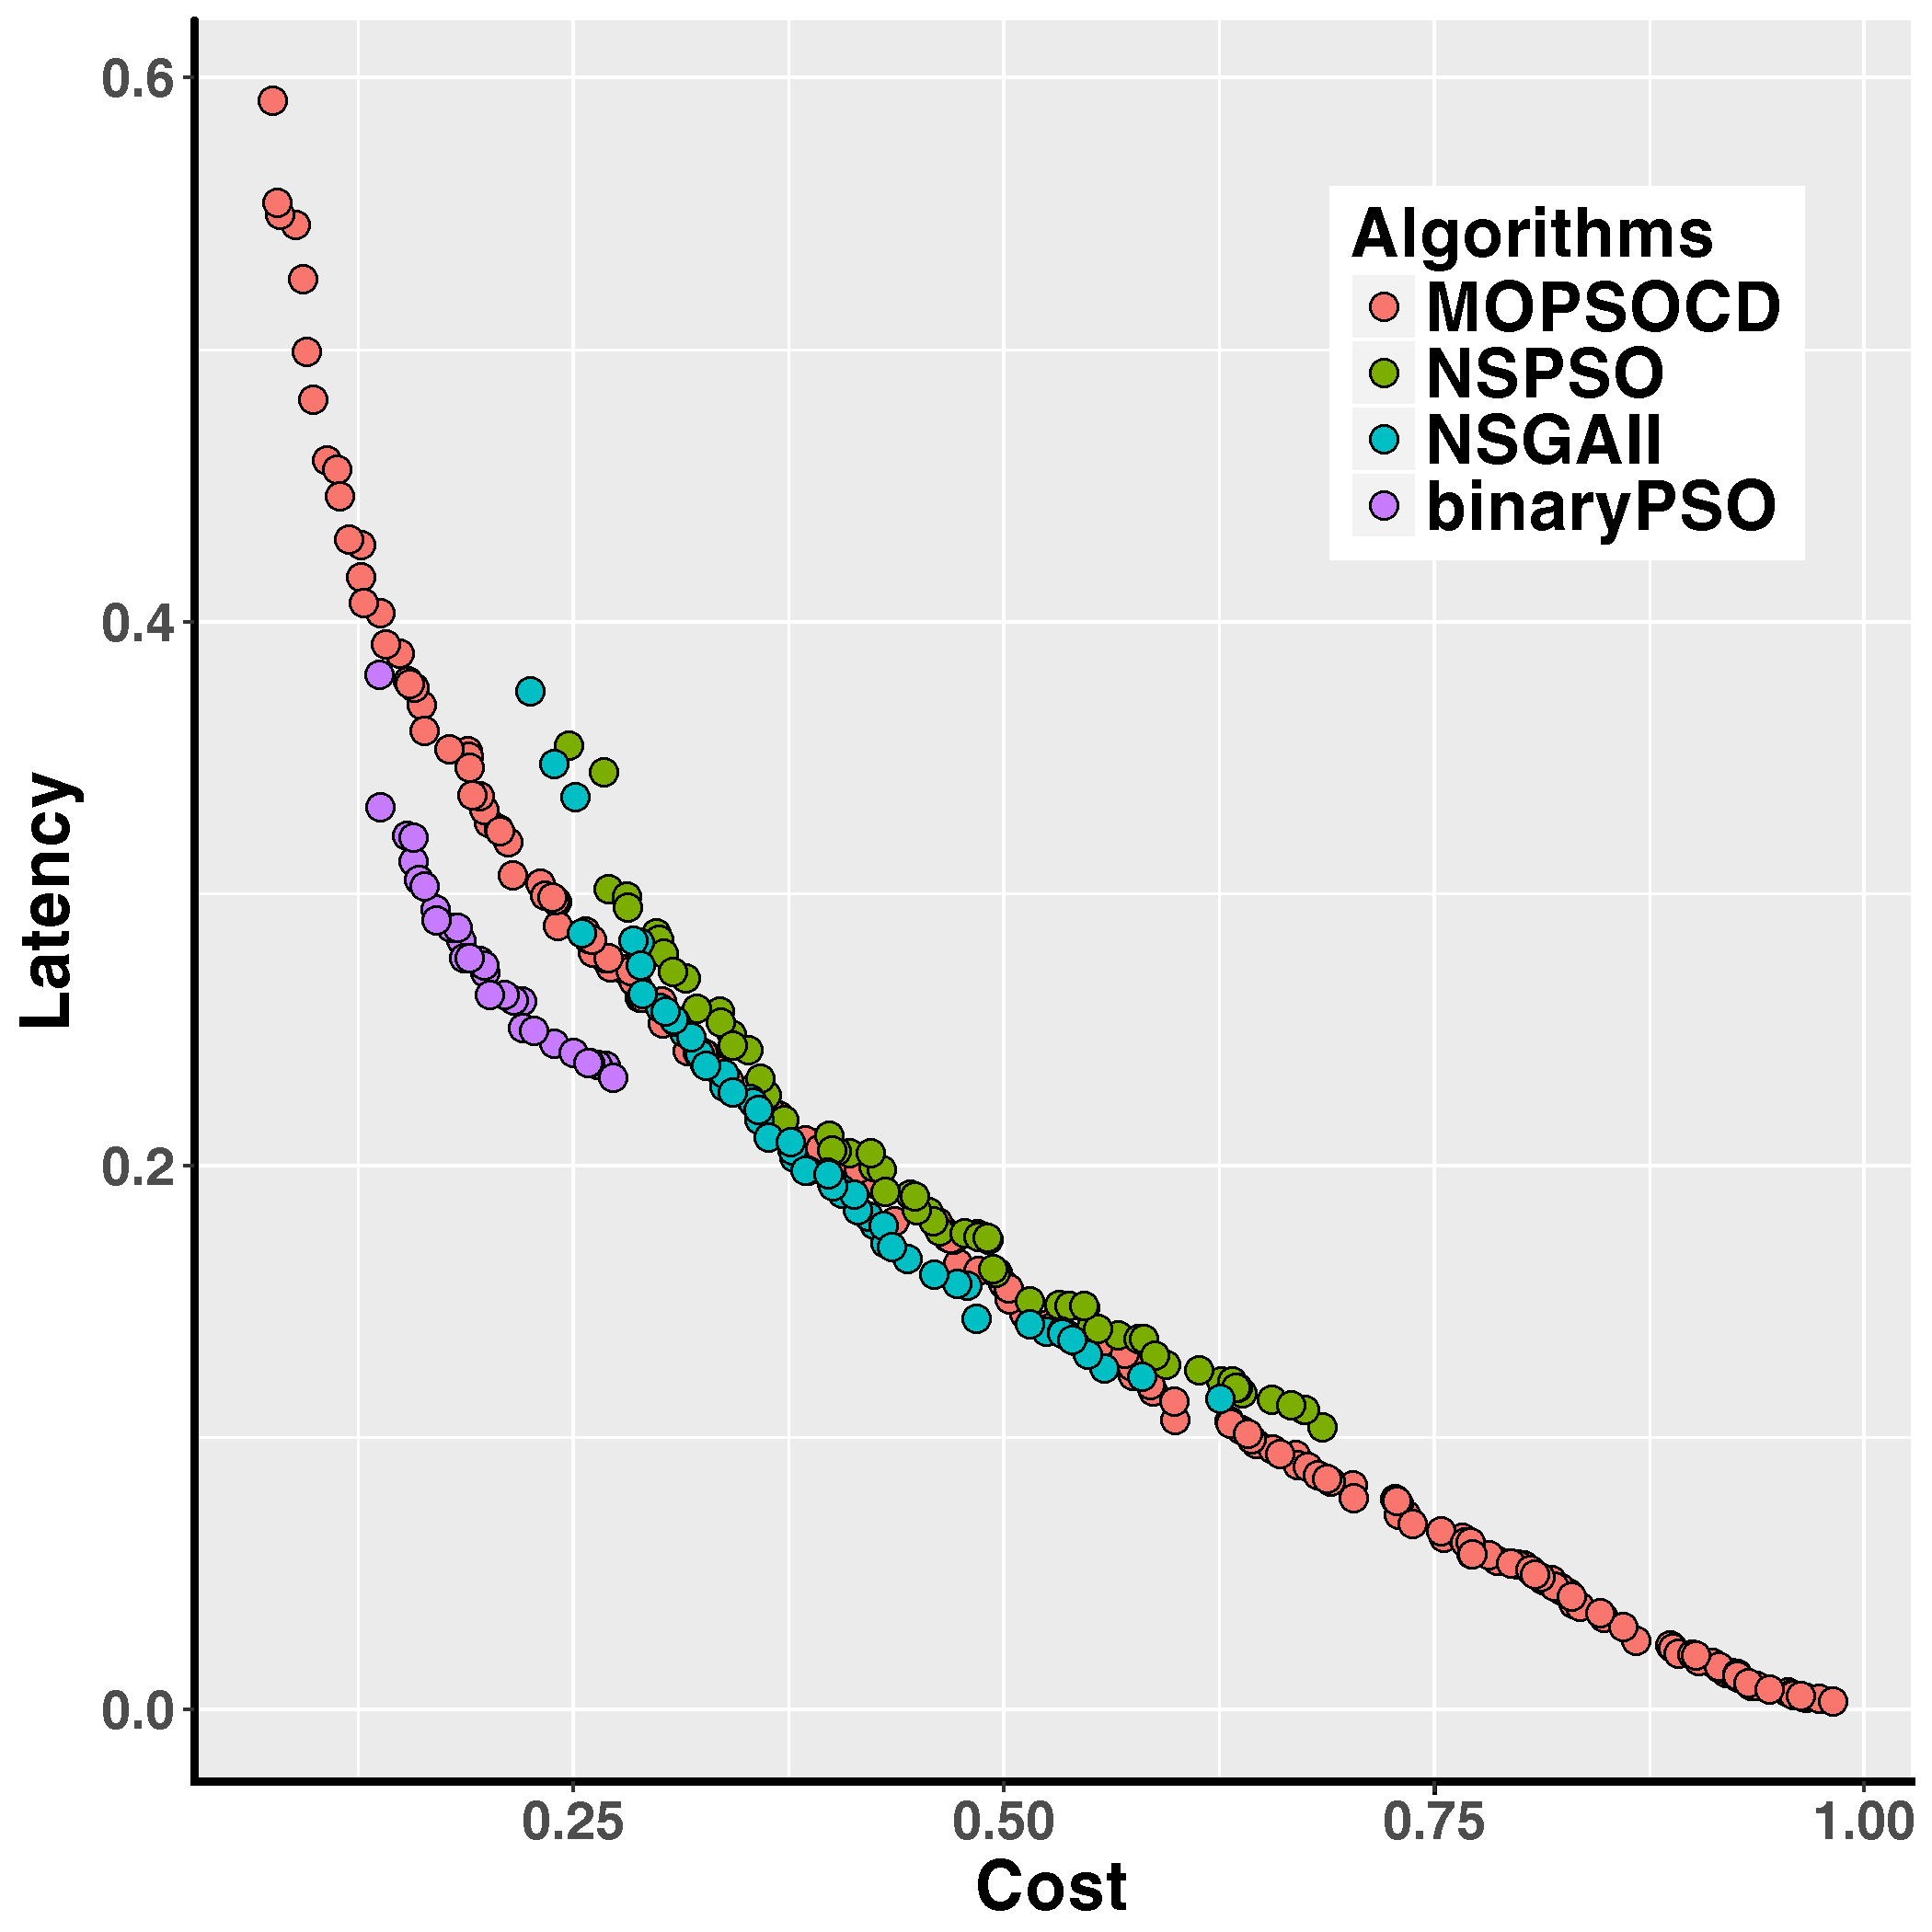
\includegraphics[width=\textwidth]{pics/total2.png}
    \caption{instance 2}
   \end{subfigure}
   \begin{subfigure}{0.21\linewidth}
       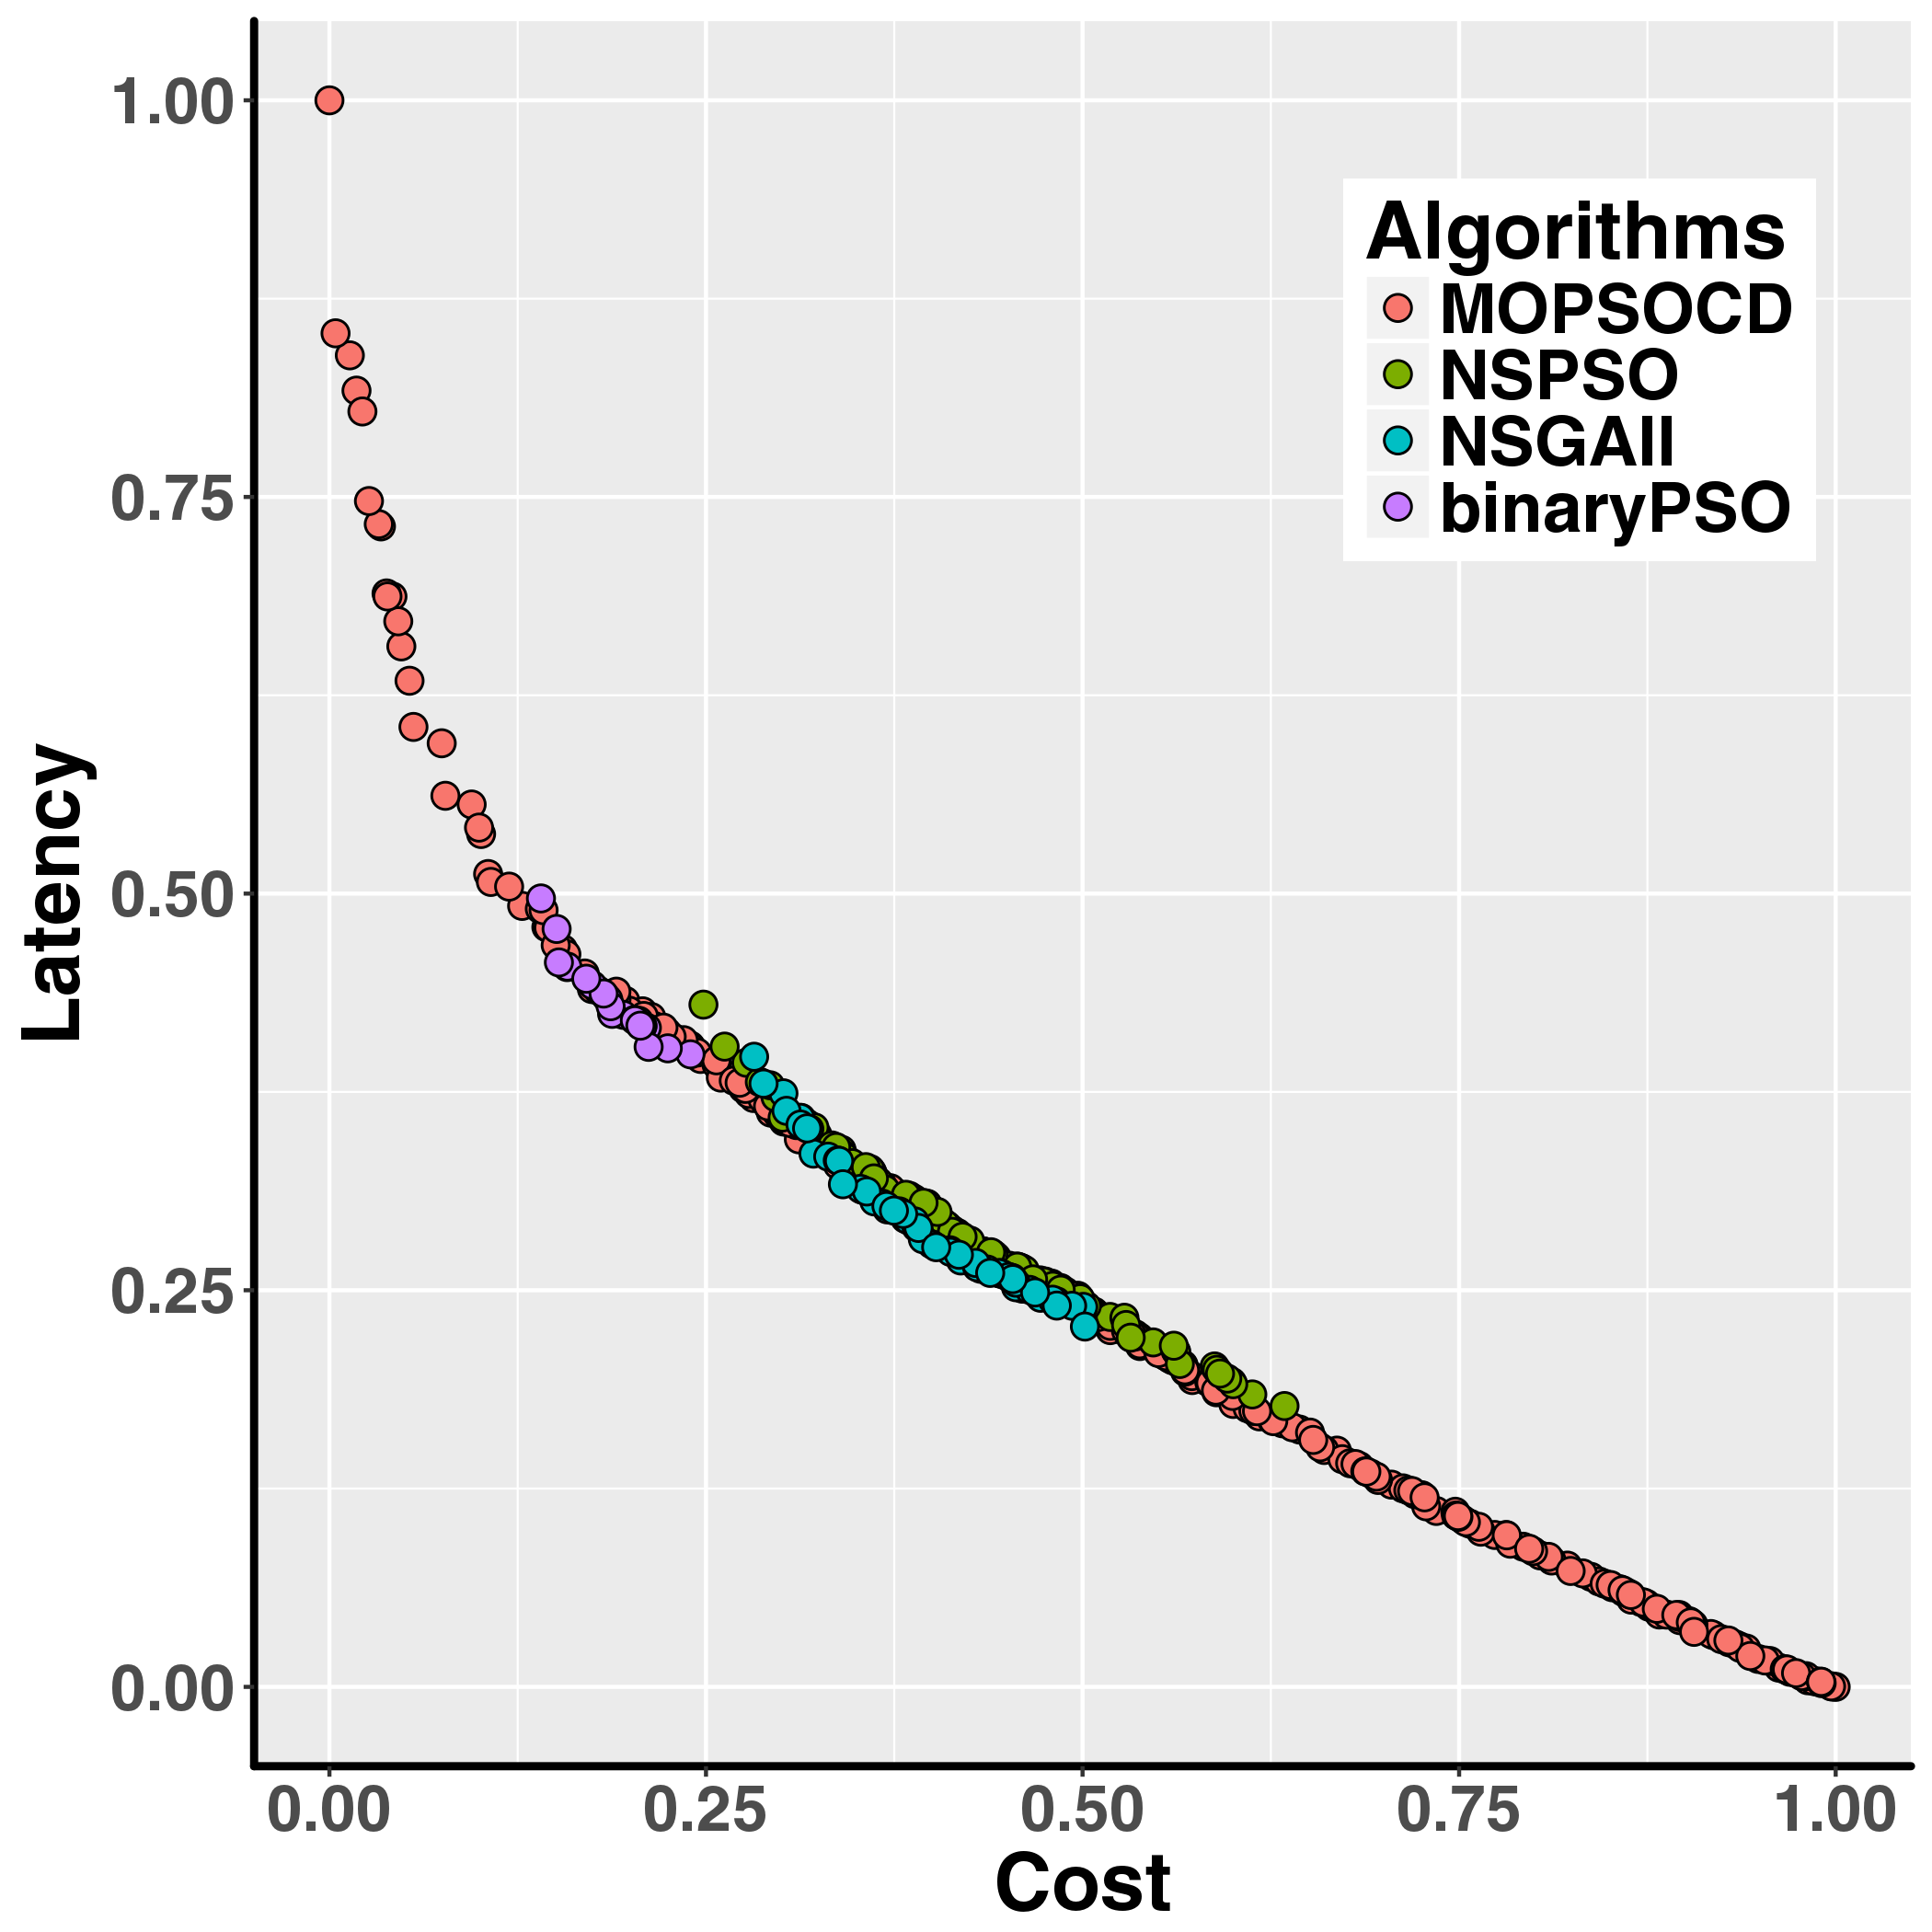
\includegraphics[width=\textwidth]{pics/total3.png}
    \caption{instance 3}
   \end{subfigure}
      \begin{subfigure}{0.21\linewidth}
       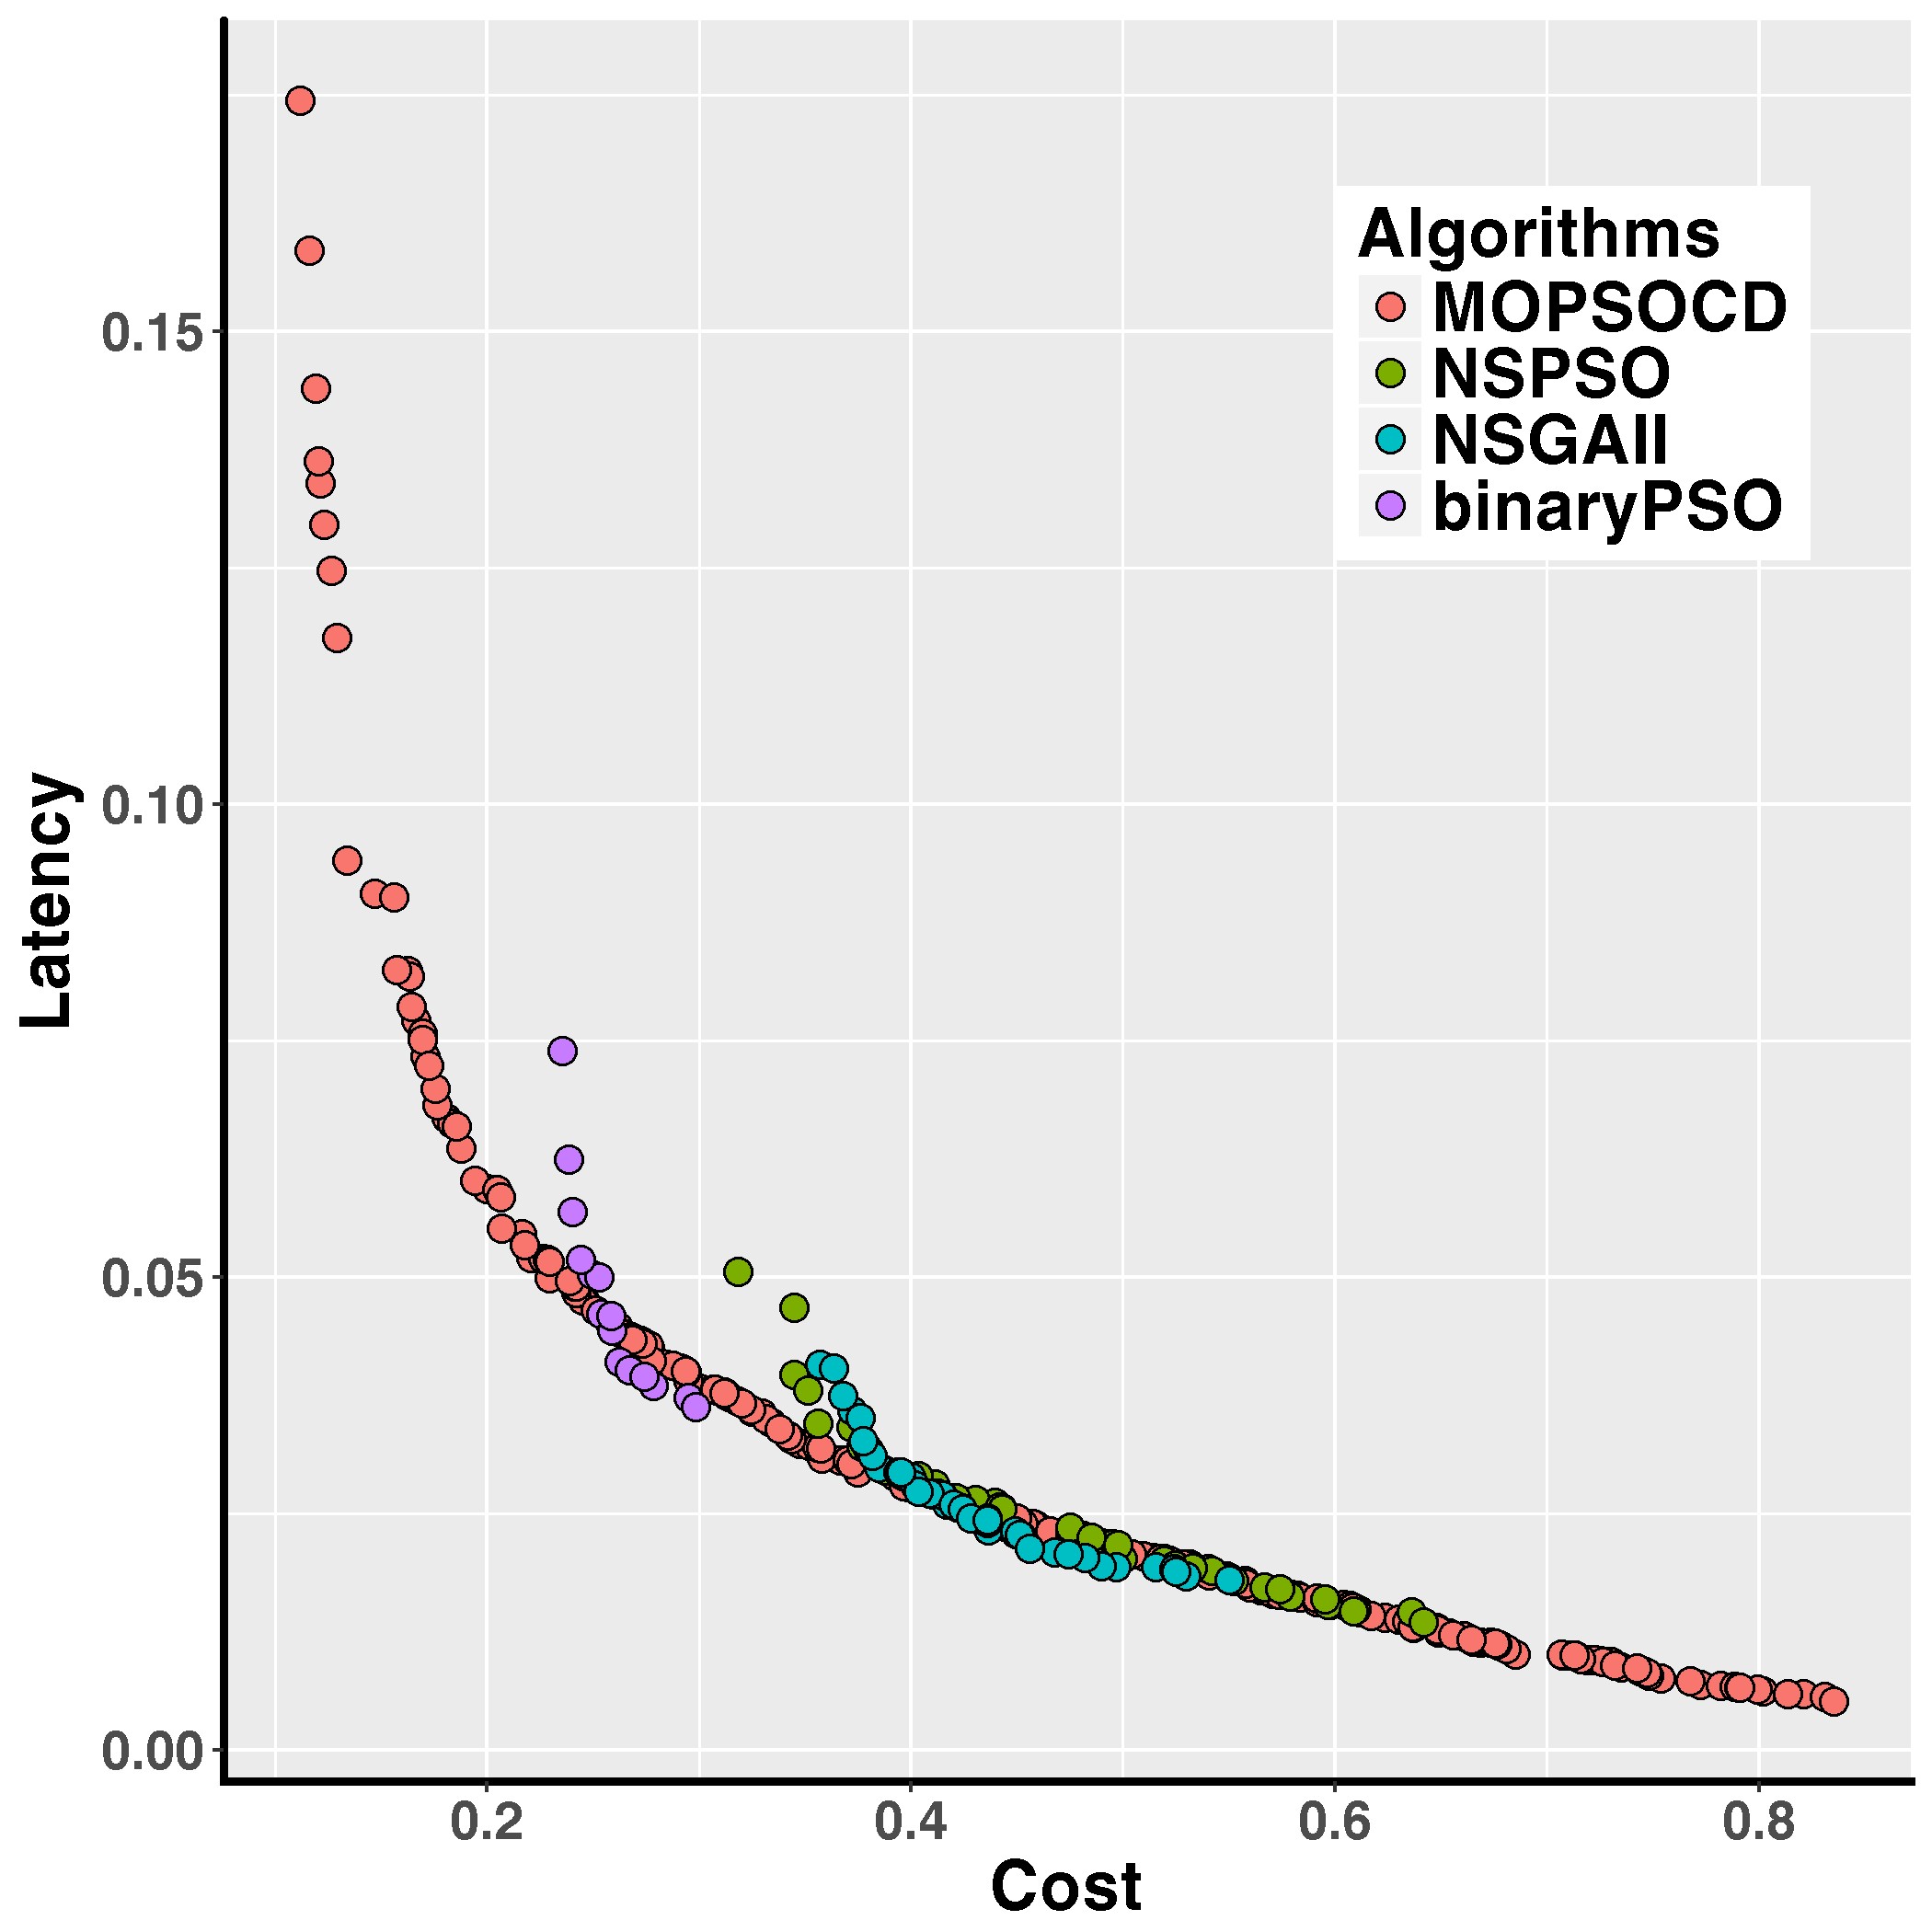
\includegraphics[width=\textwidth]{pics/total4.png}
    \caption{instance 4}
   \end{subfigure}
      \begin{subfigure}{0.21\linewidth}
       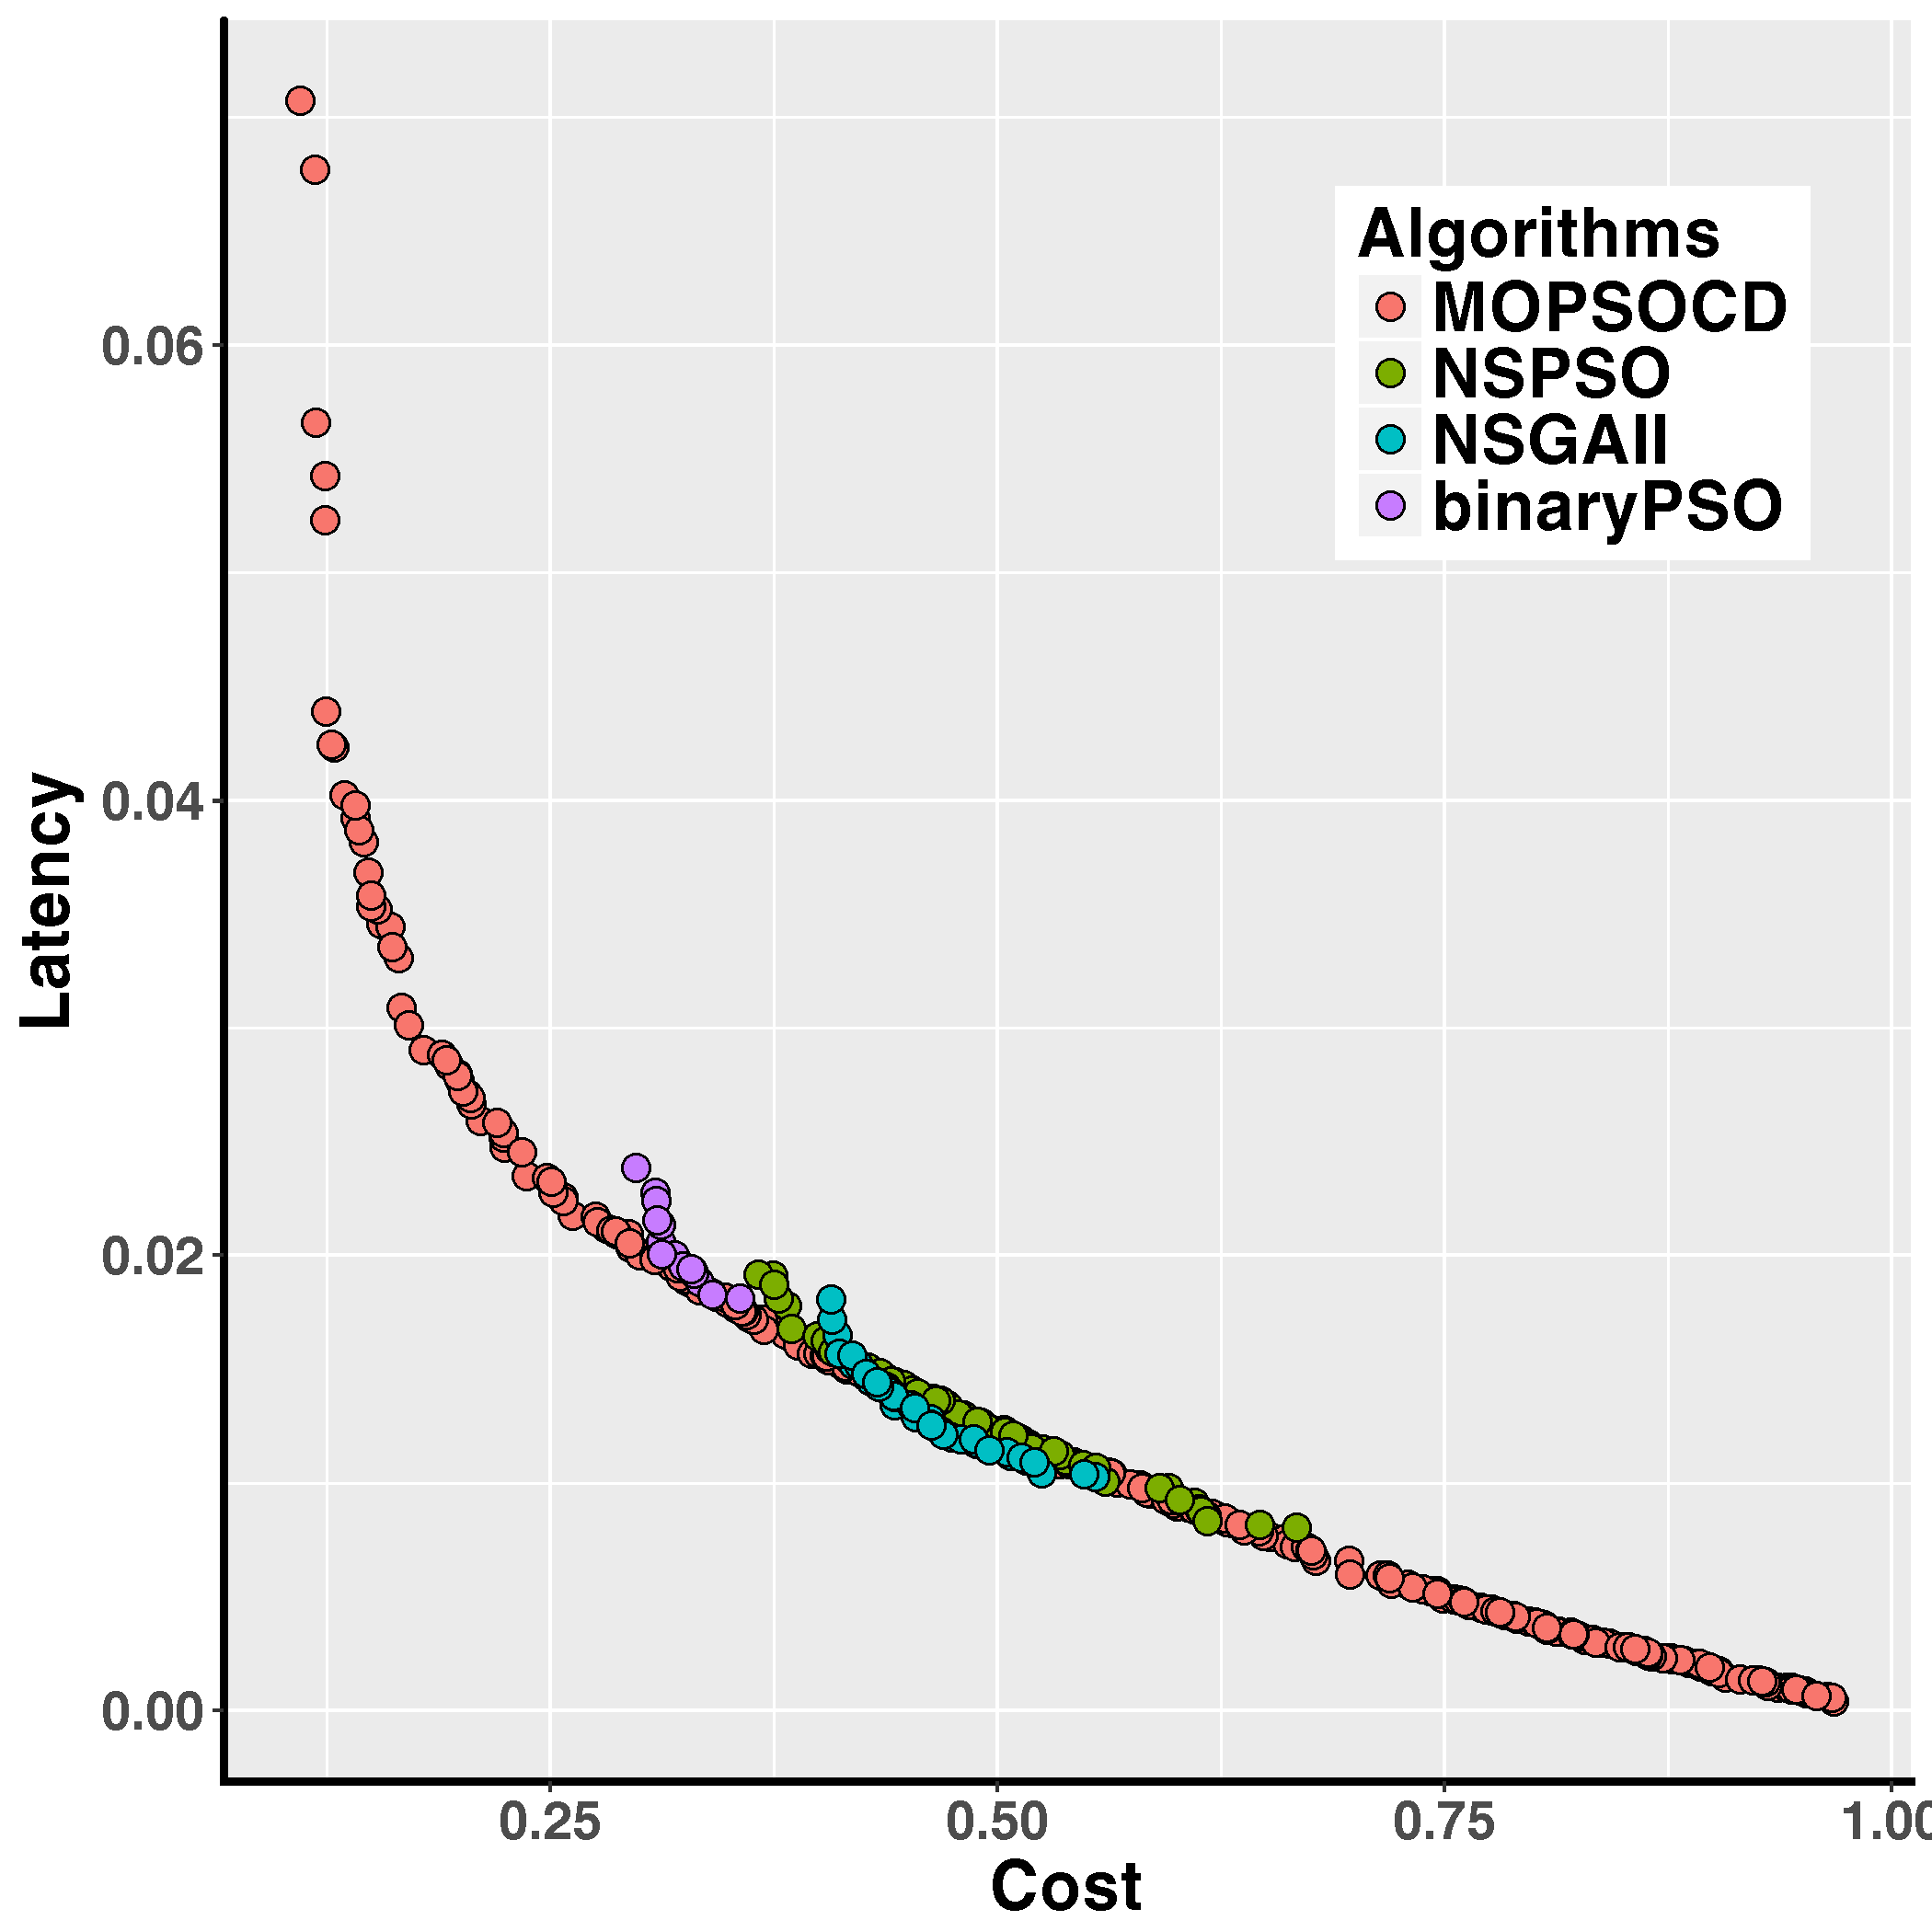
\includegraphics[width=\textwidth]{pics/total5.png}
    \caption{instance 5}
   \end{subfigure}
   \begin{subfigure}{0.21\linewidth}
       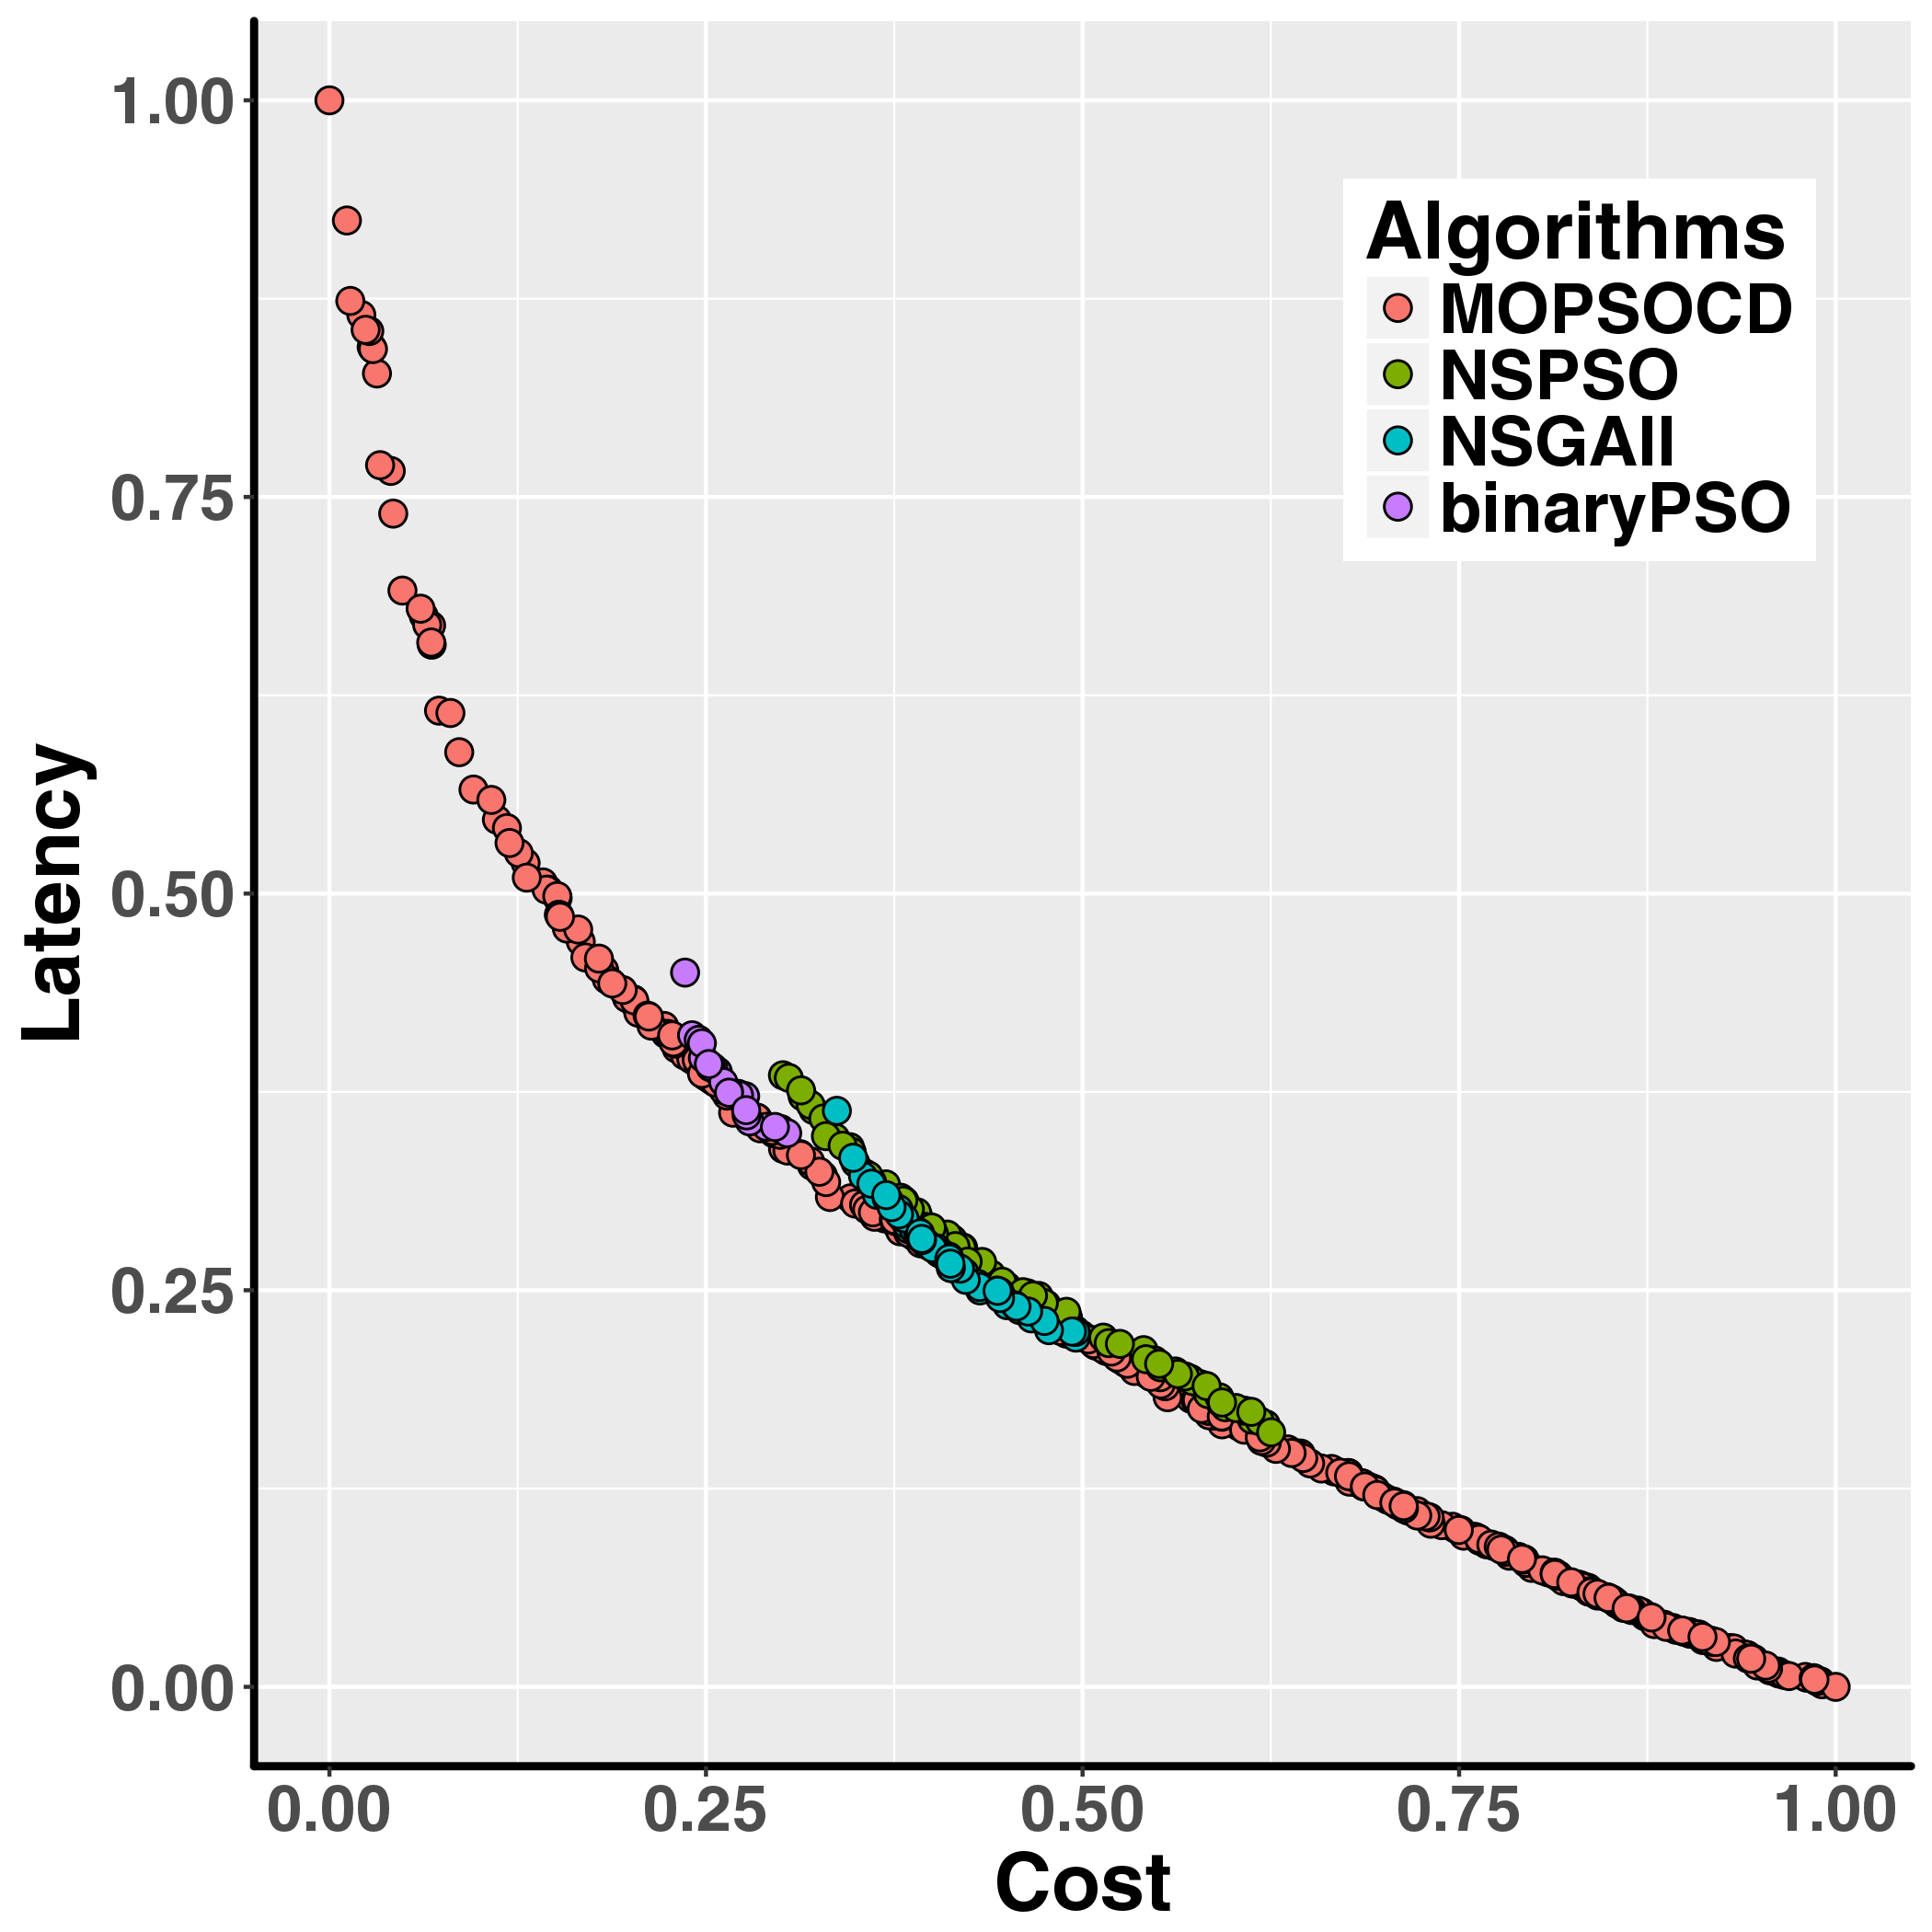
\includegraphics[width=\textwidth]{pics/total6.png}
    \caption{instance 6}
   \end{subfigure}
   \begin{subfigure}{0.21\linewidth}
       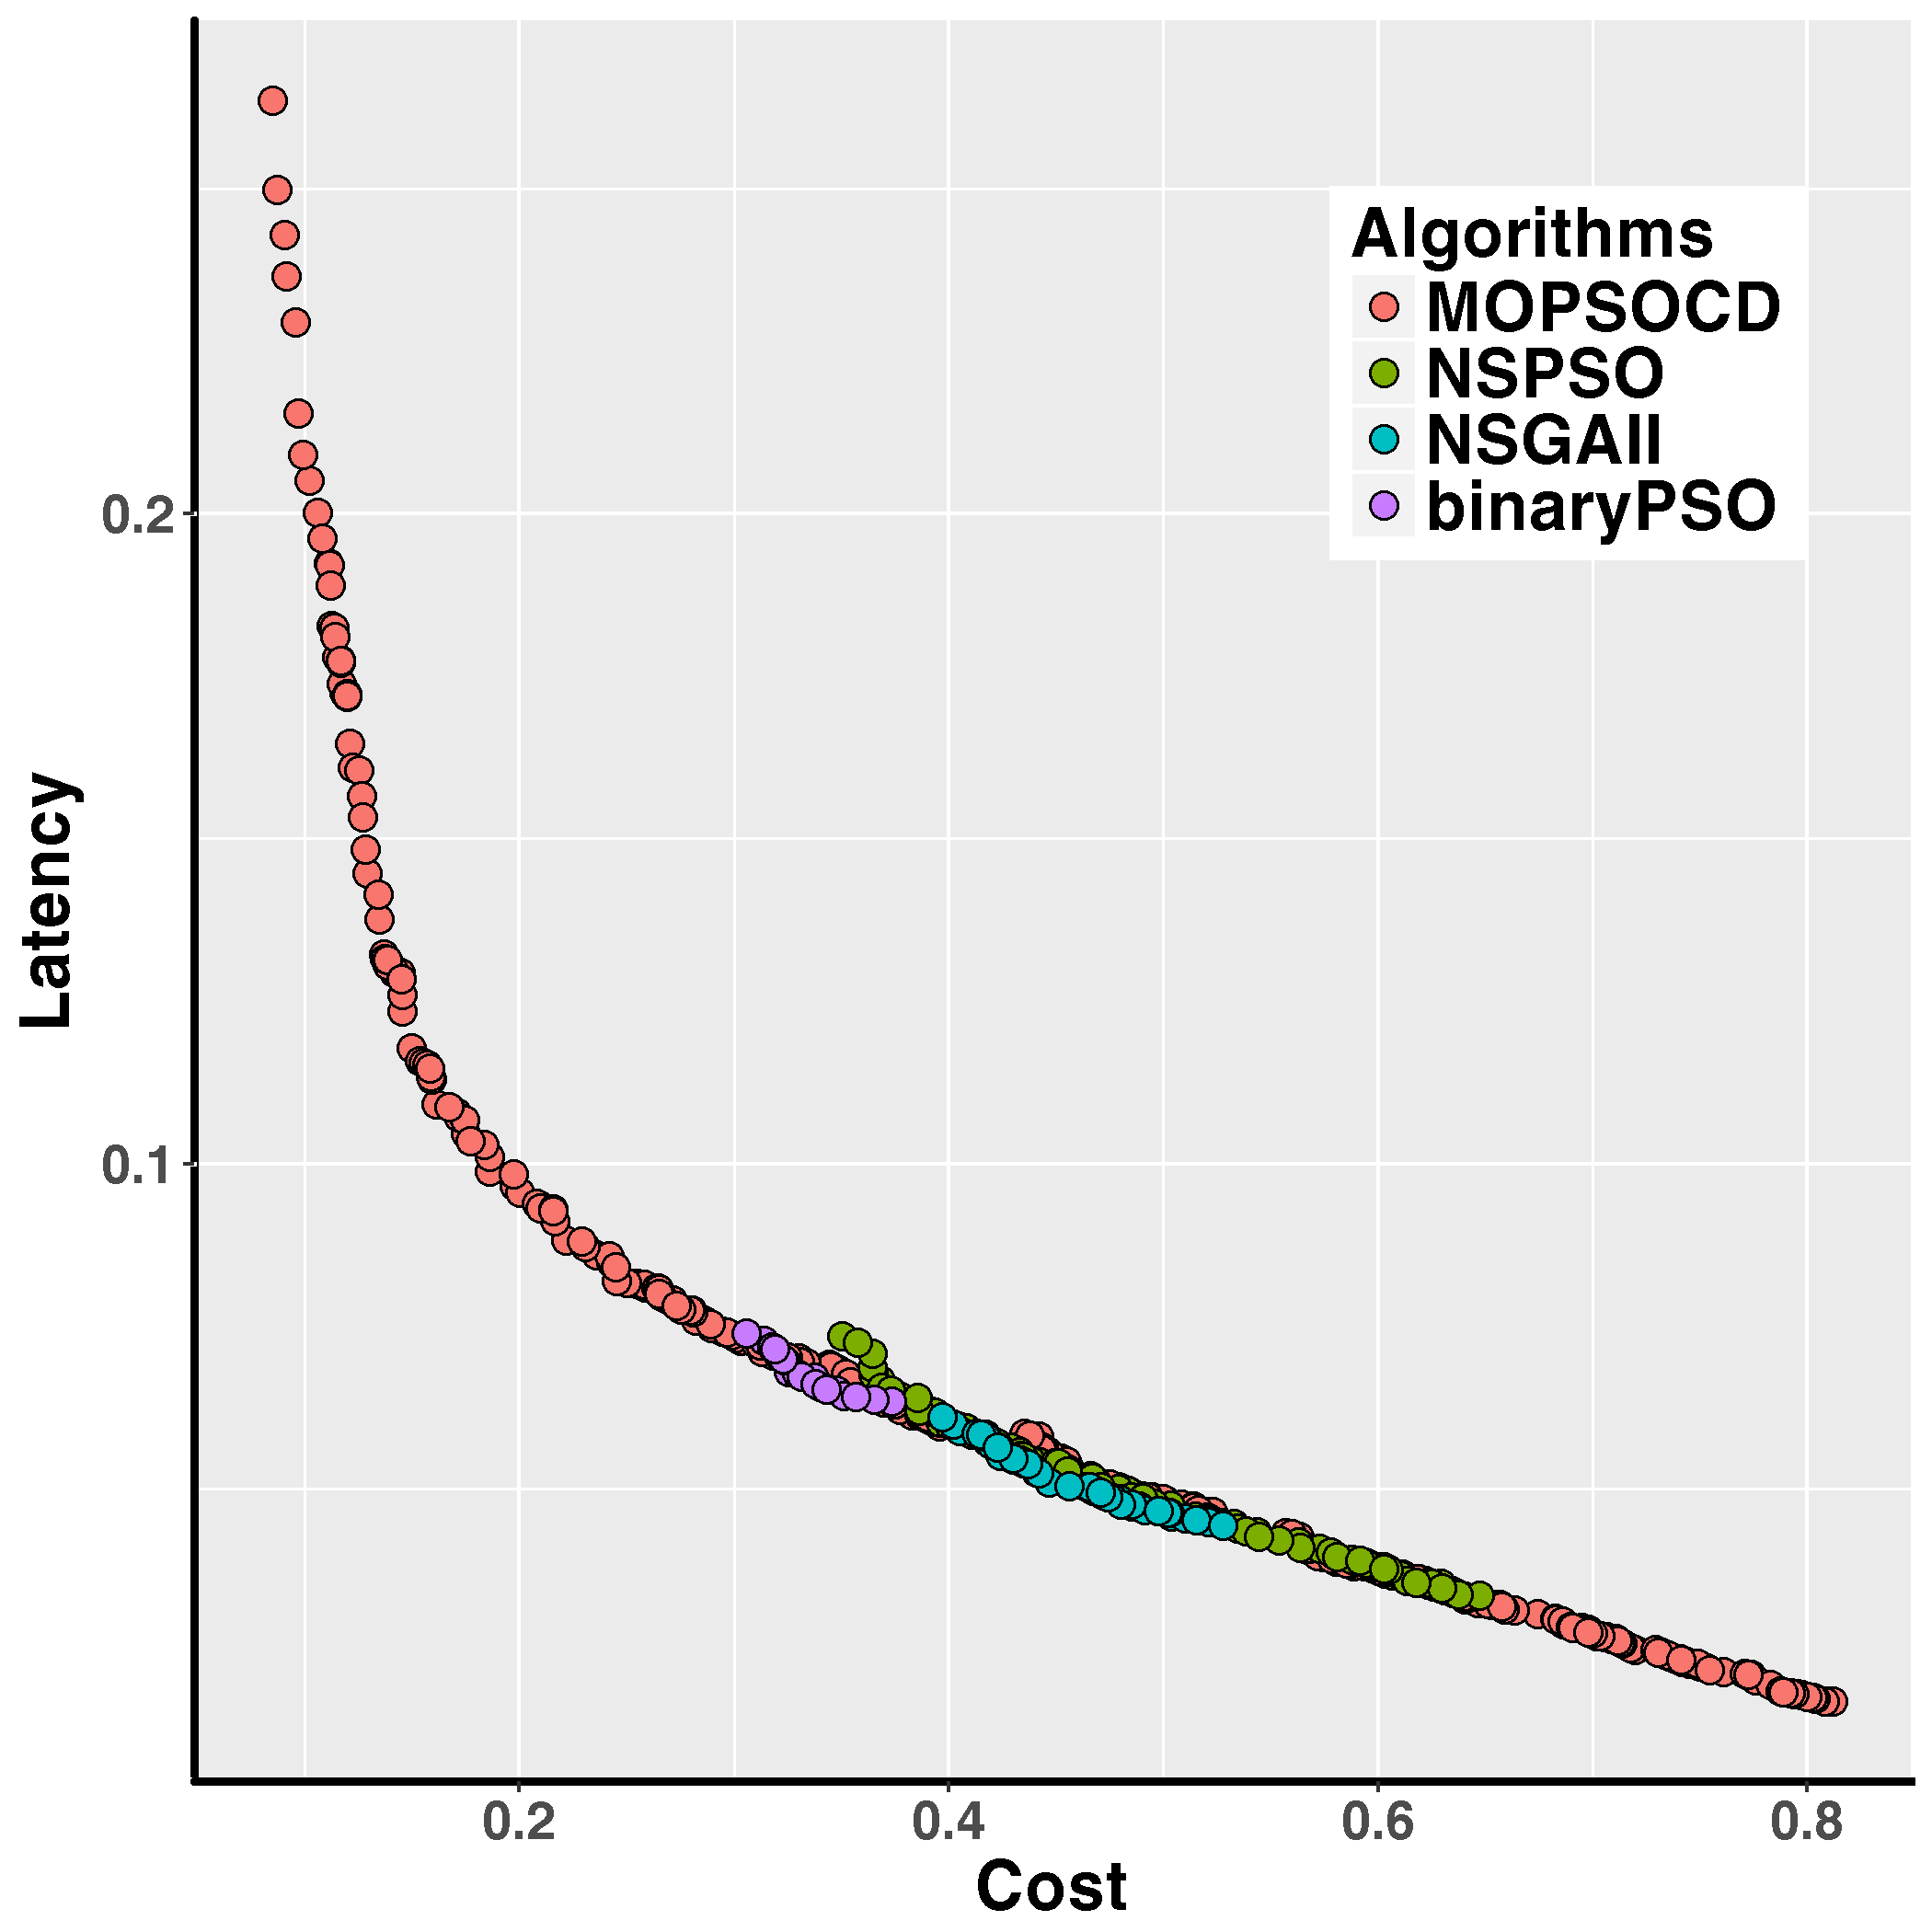
\includegraphics[width=\textwidth]{pics/total7.png}
    \caption{instance 7}
   \end{subfigure}
      \begin{subfigure}{0.21\linewidth}
       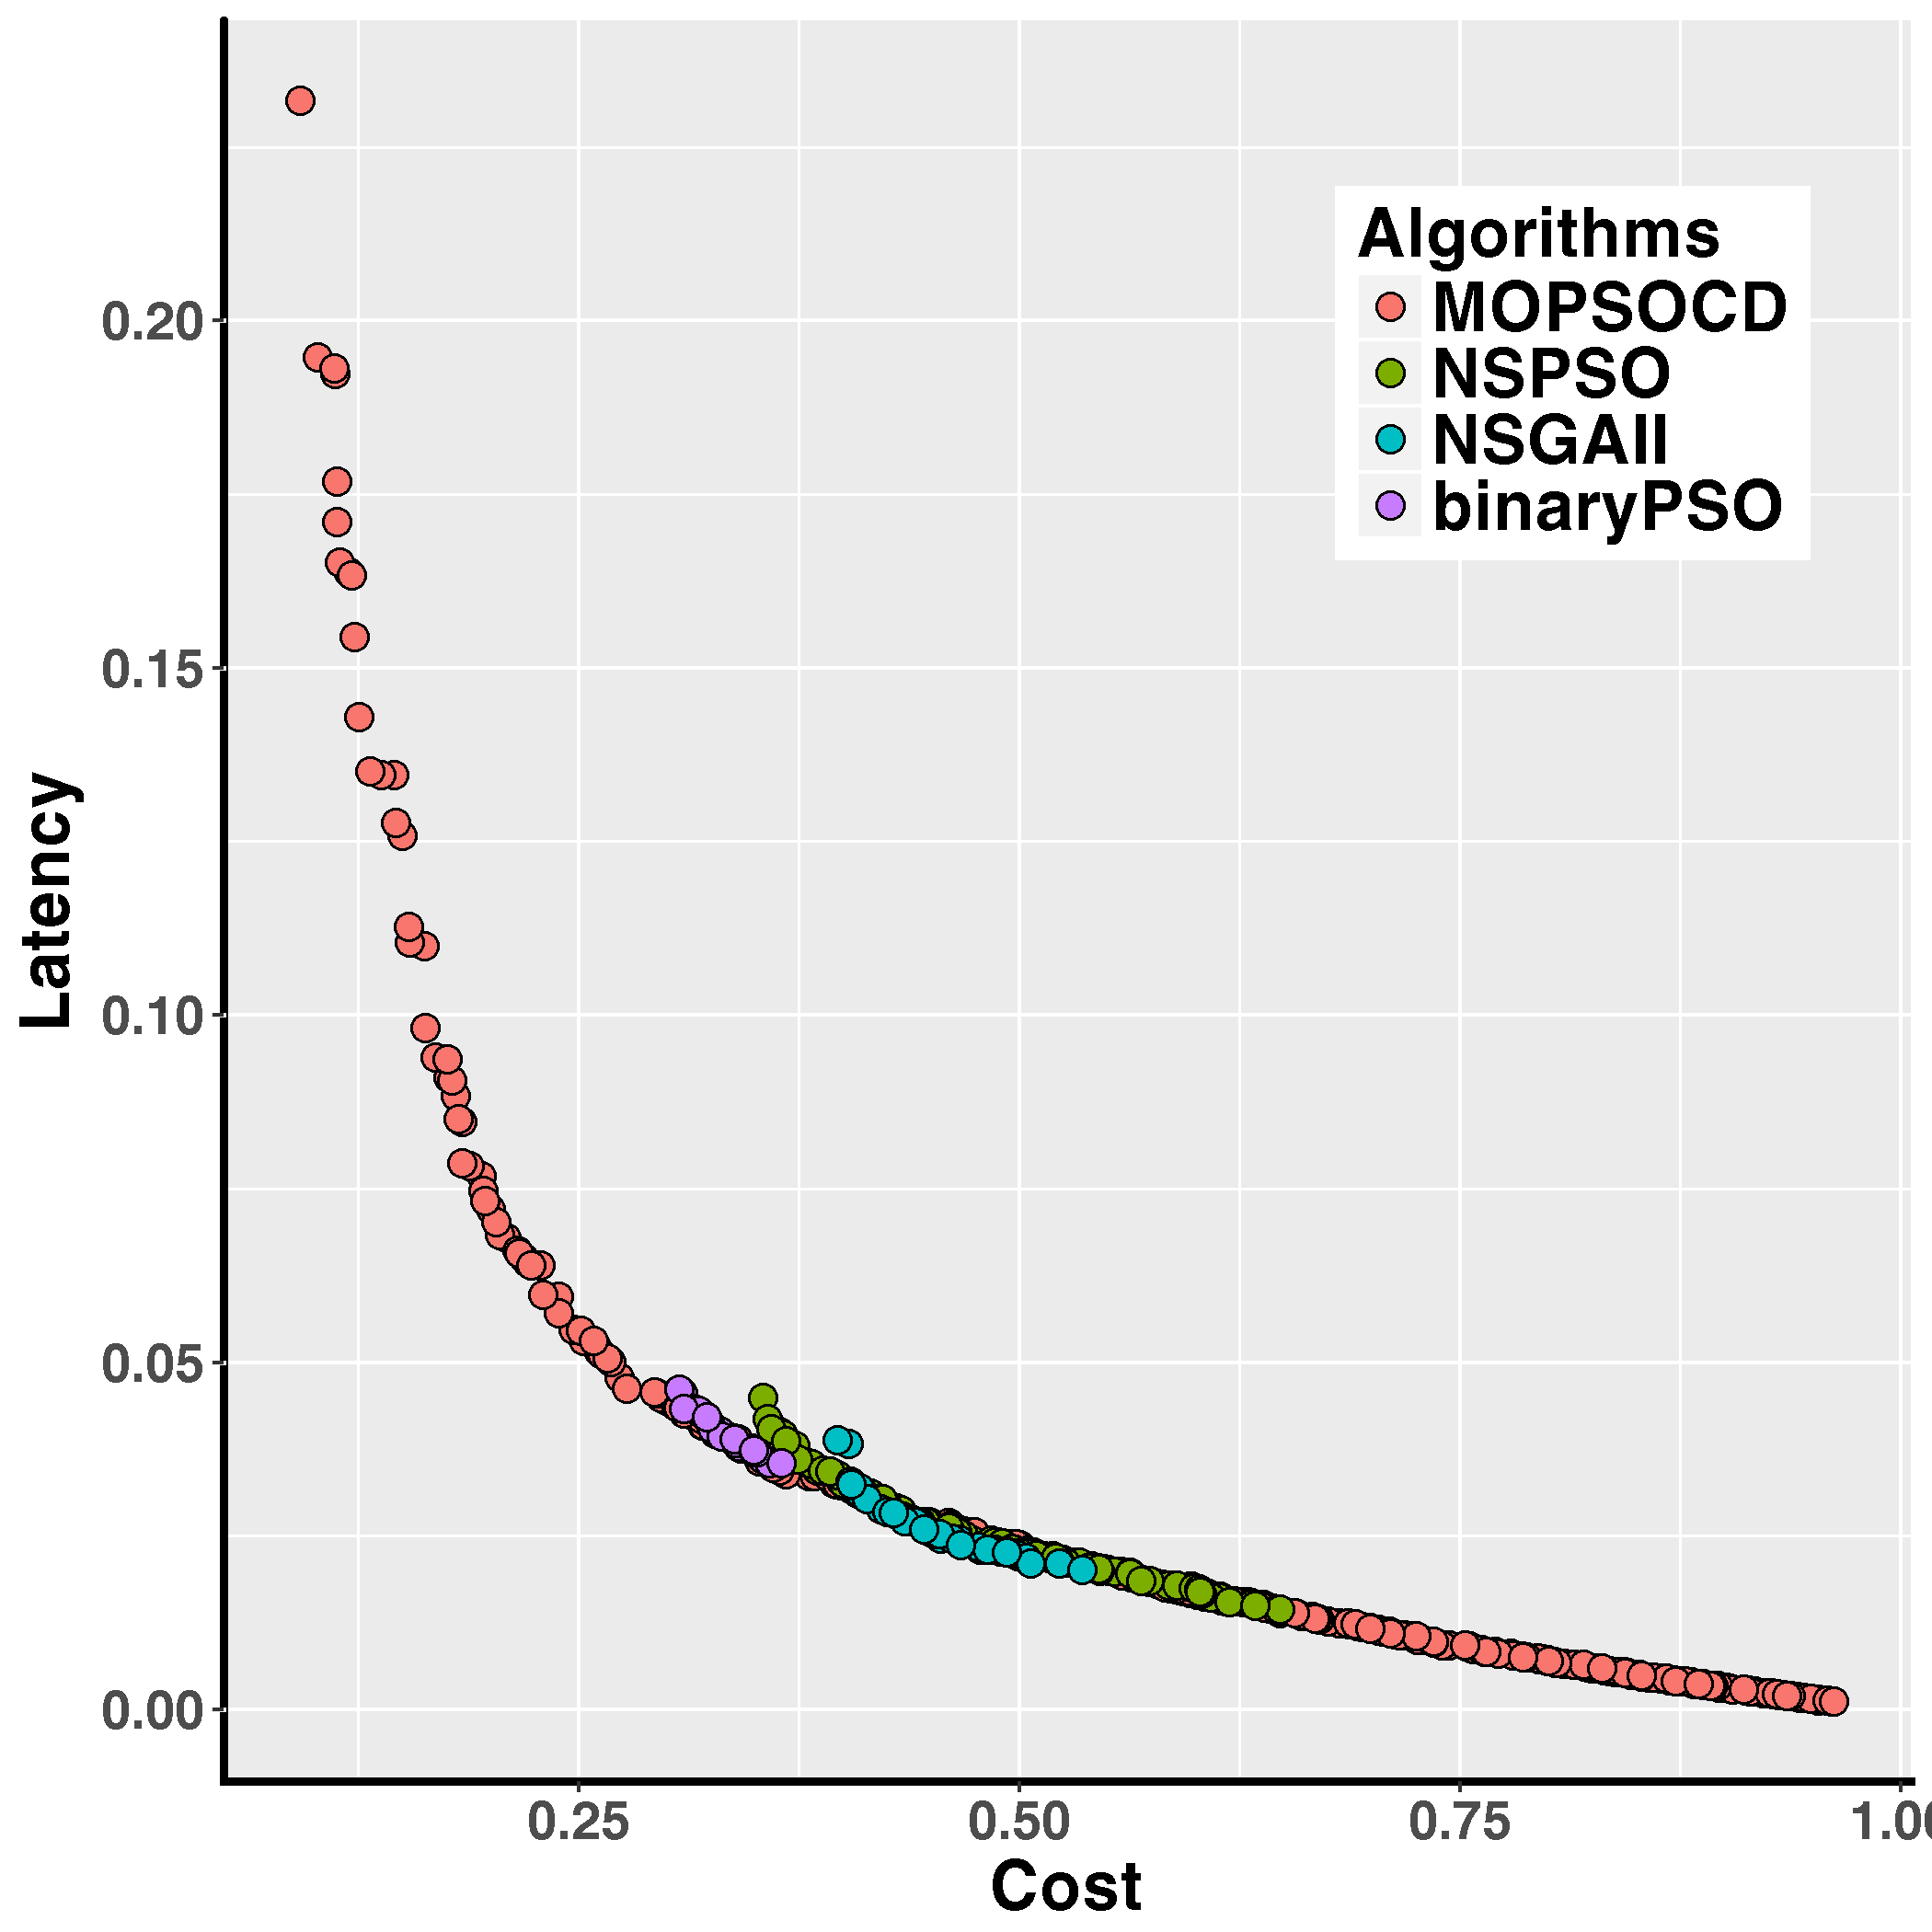
\includegraphics[width=\textwidth]{pics/total8.png}
    \caption{instance 8}
   \end{subfigure}
      \begin{subfigure}{0.21\linewidth}
       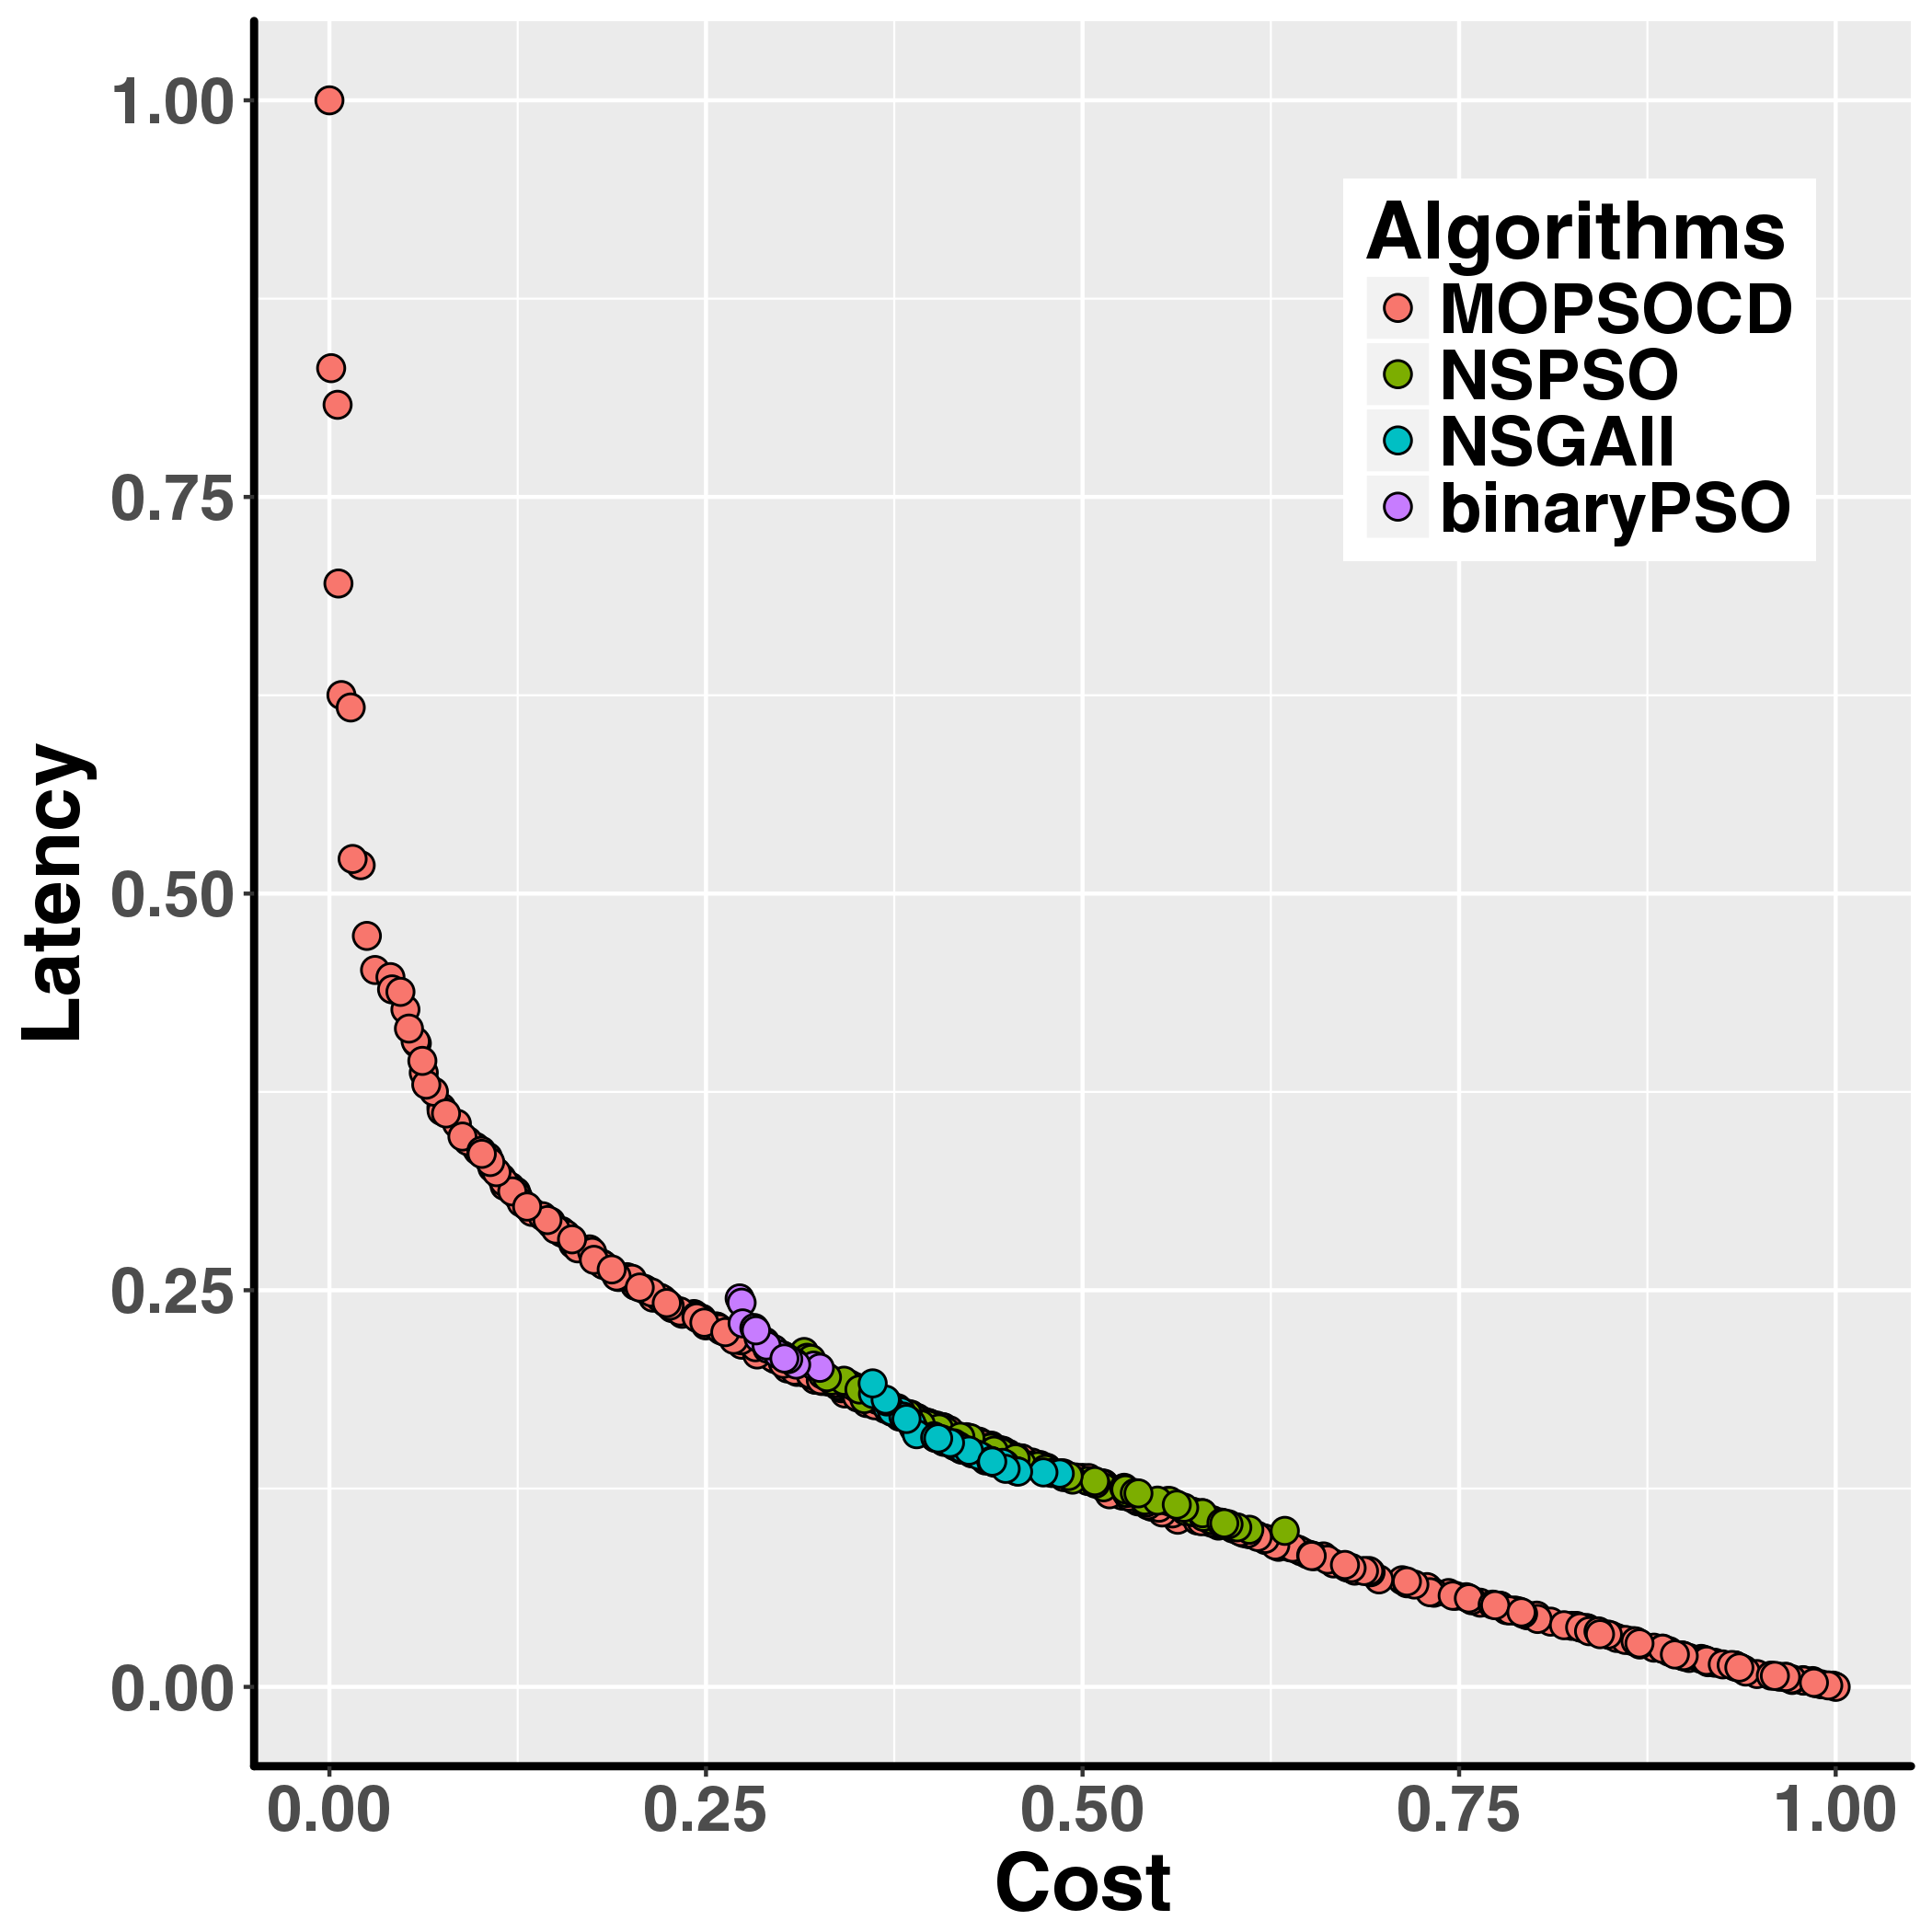
\includegraphics[width=\textwidth]{pics/total9.png}
    \caption{instance 9}
   \end{subfigure}
   \begin{subfigure}{0.21\linewidth}
       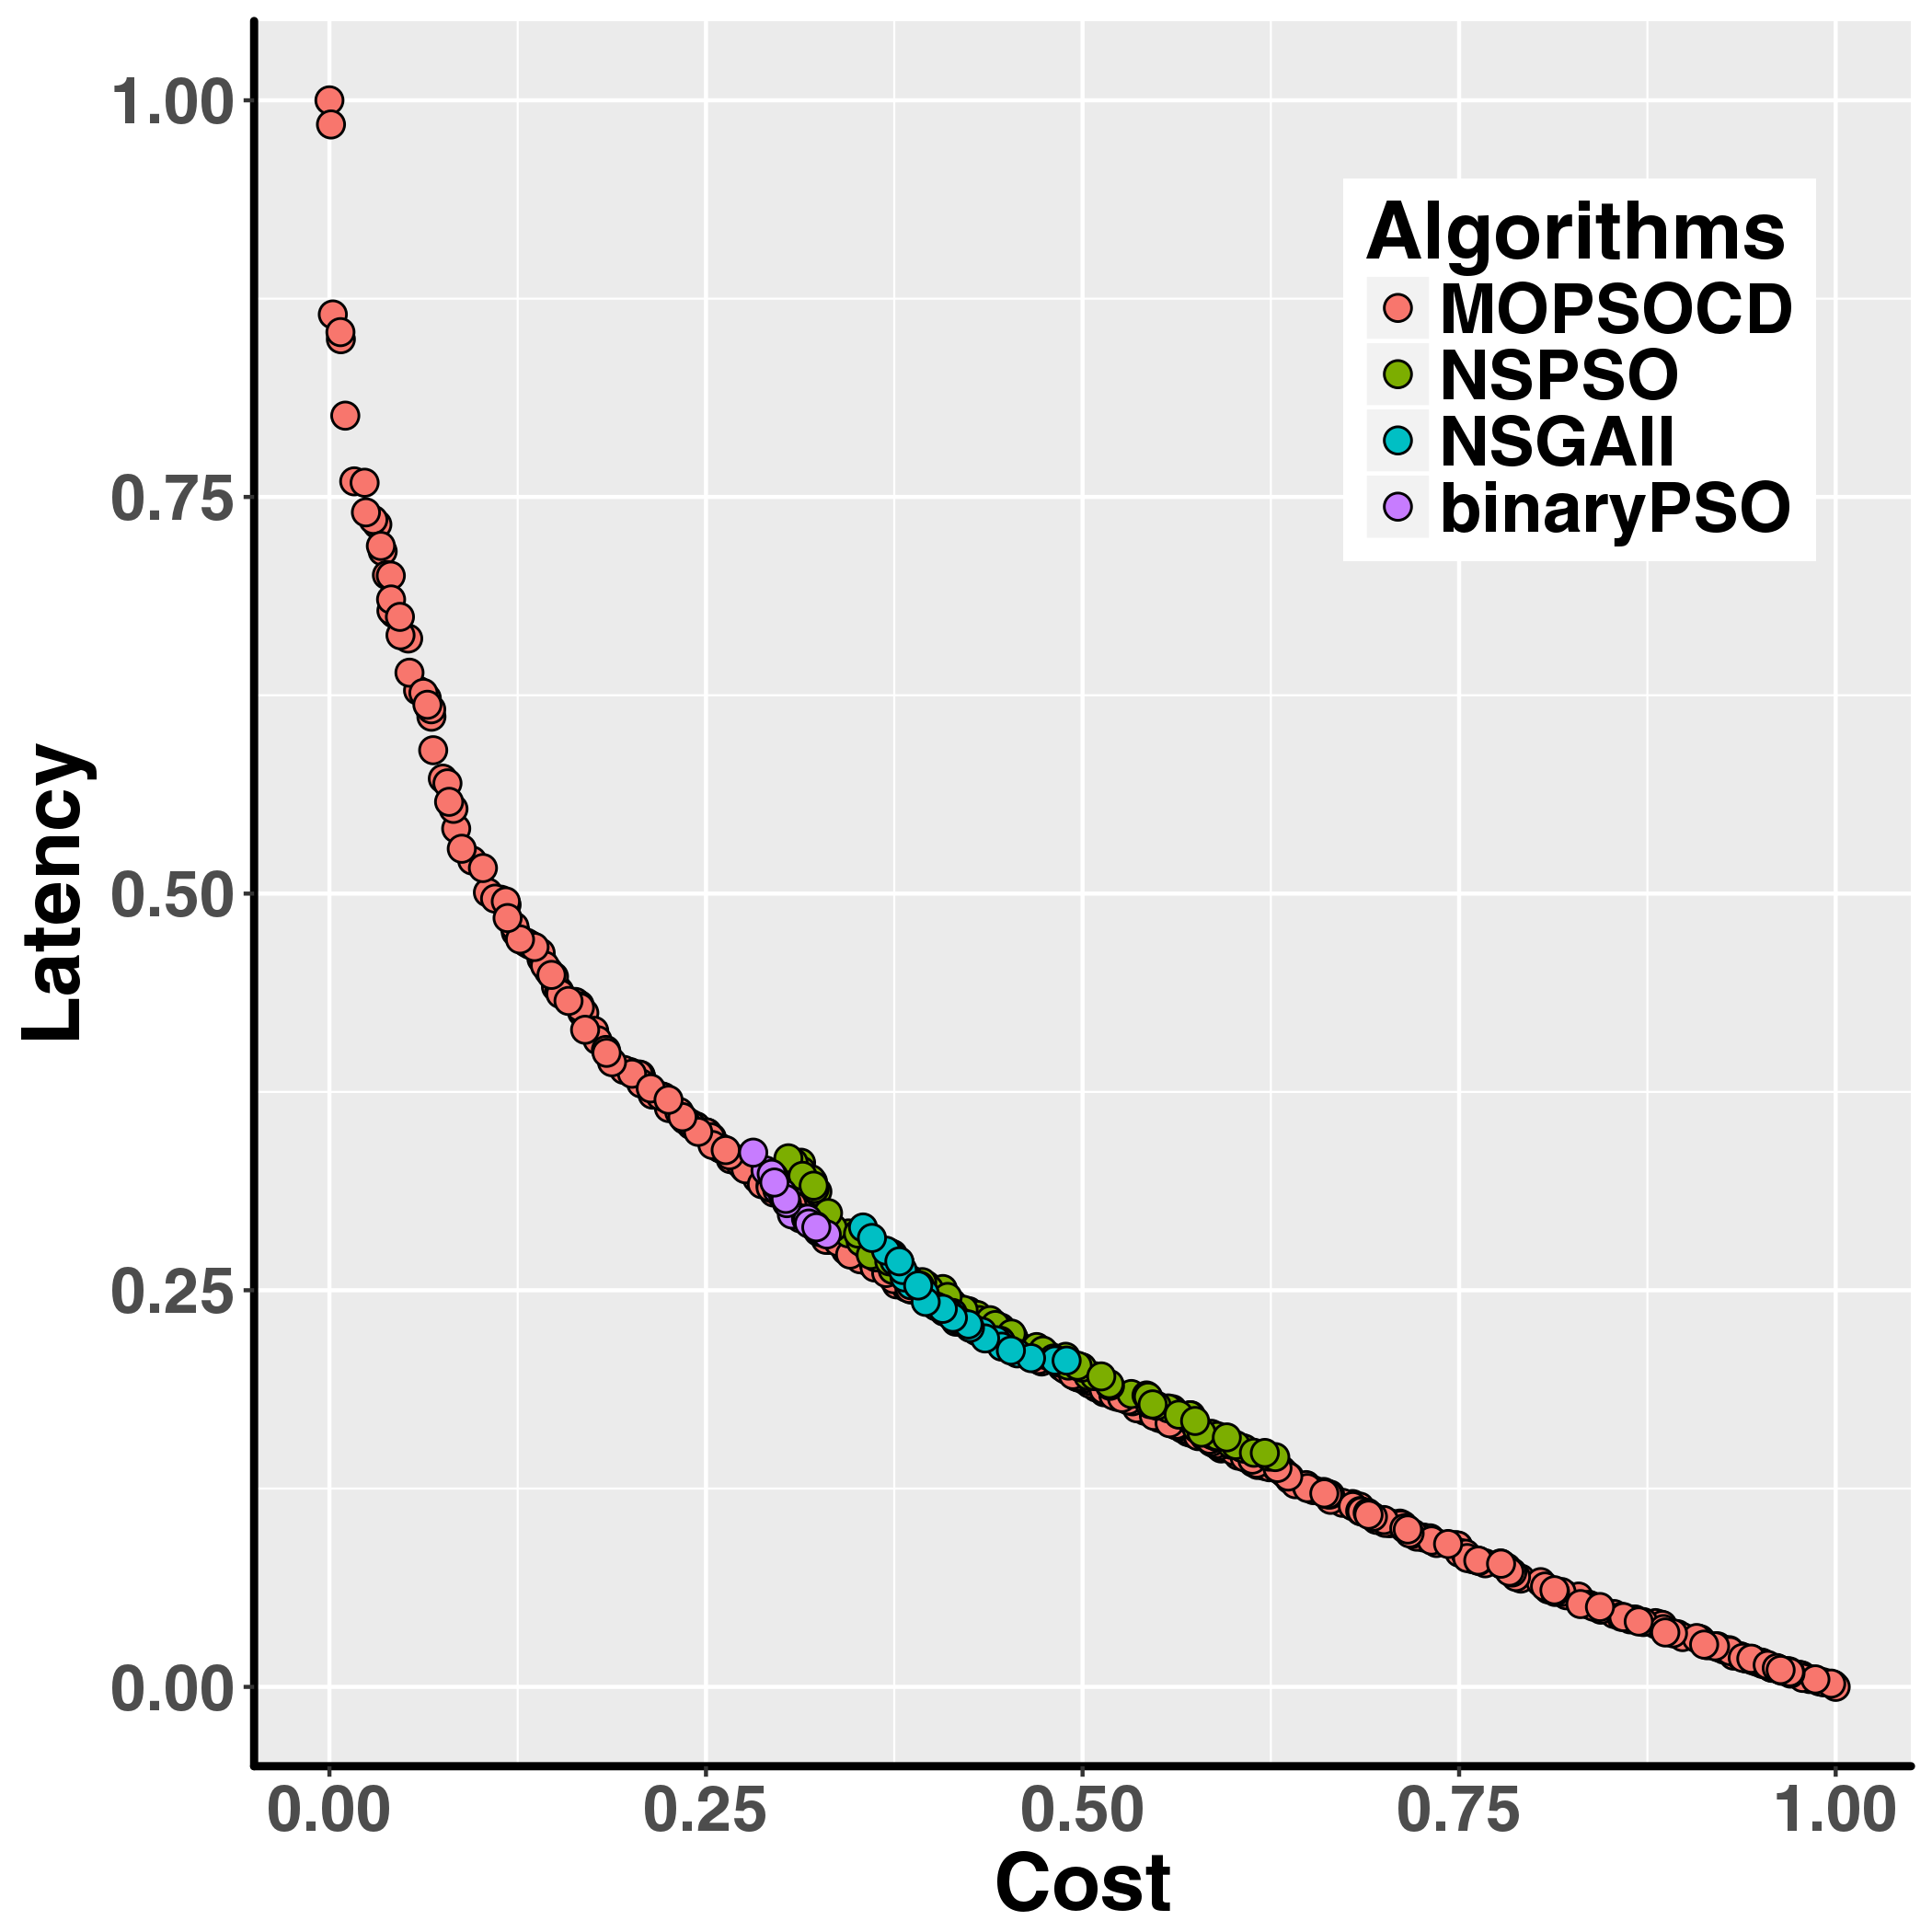
\includegraphics[width=\textwidth]{pics/total10.png}
    \caption{instance 10}
   \end{subfigure}
   \begin{subfigure}{0.21\linewidth}
       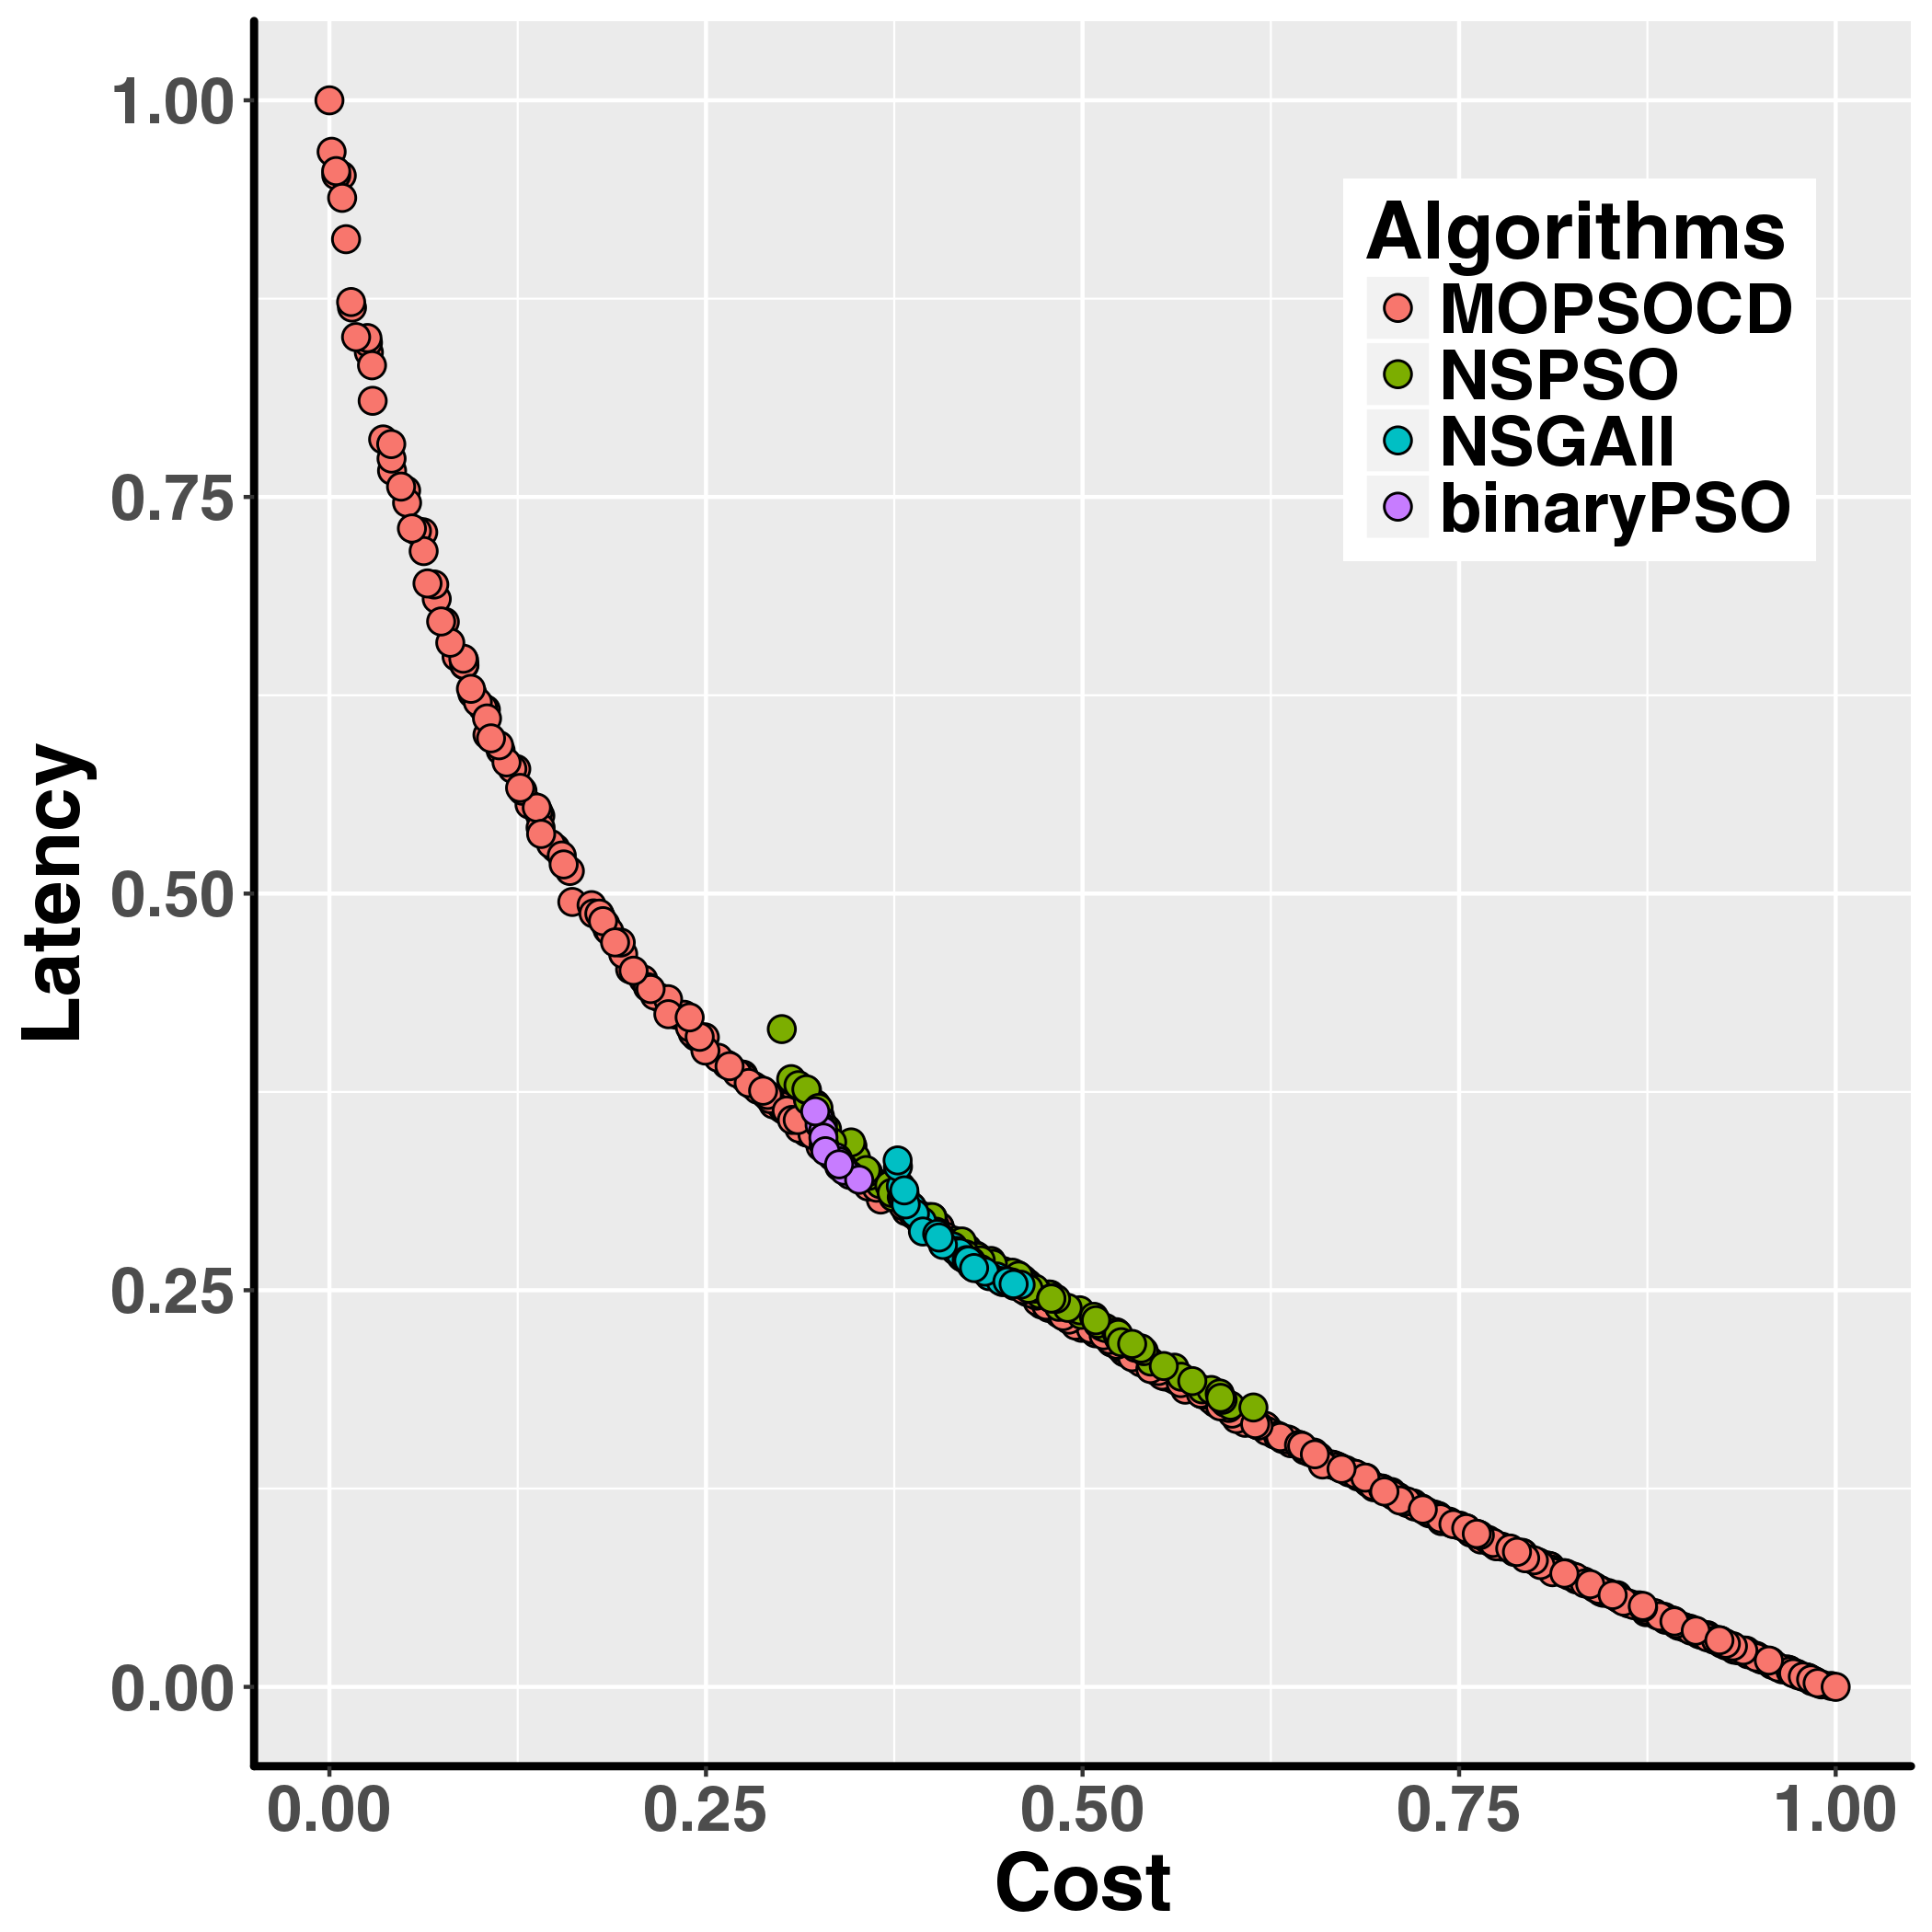
\includegraphics[width=\textwidth]{pics/total11.png}
    \caption{instance 11}
   \end{subfigure}
   \begin{subfigure}{0.21\linewidth}
       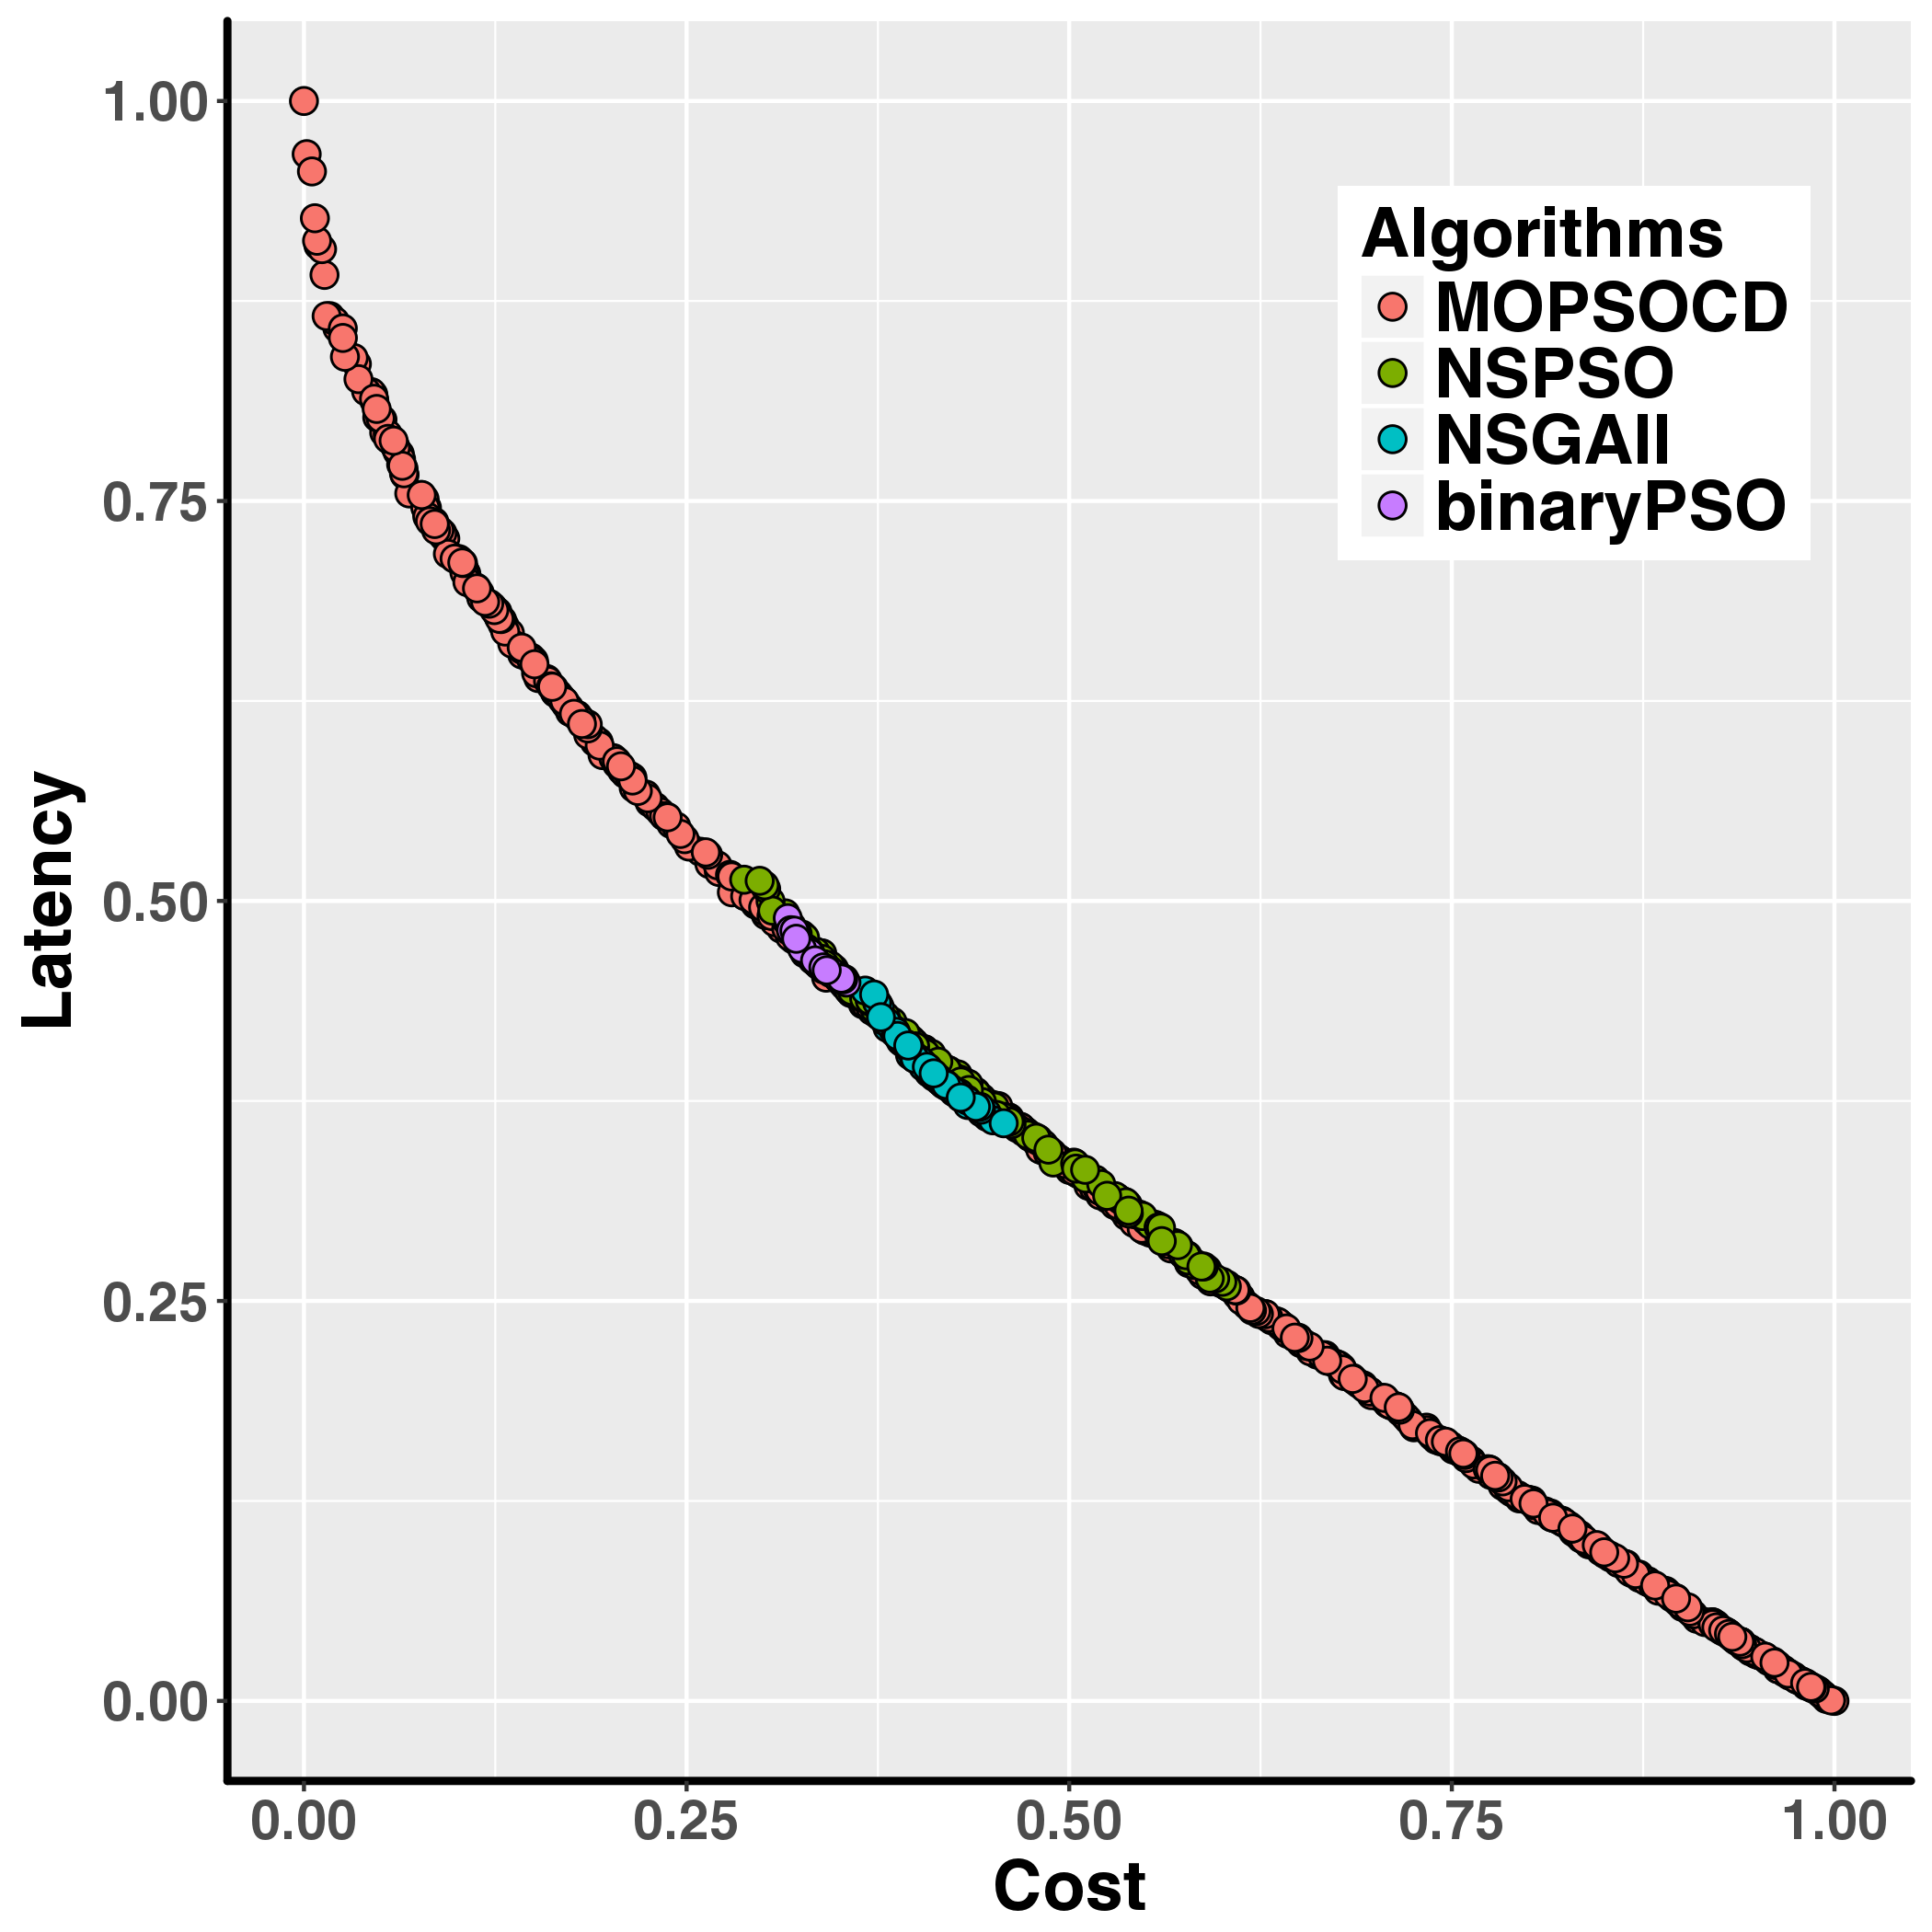
\includegraphics[width=\textwidth]{pics/total12.png}
    \caption{instance 12}
   \end{subfigure}
      \begin{subfigure}{0.21\linewidth}
       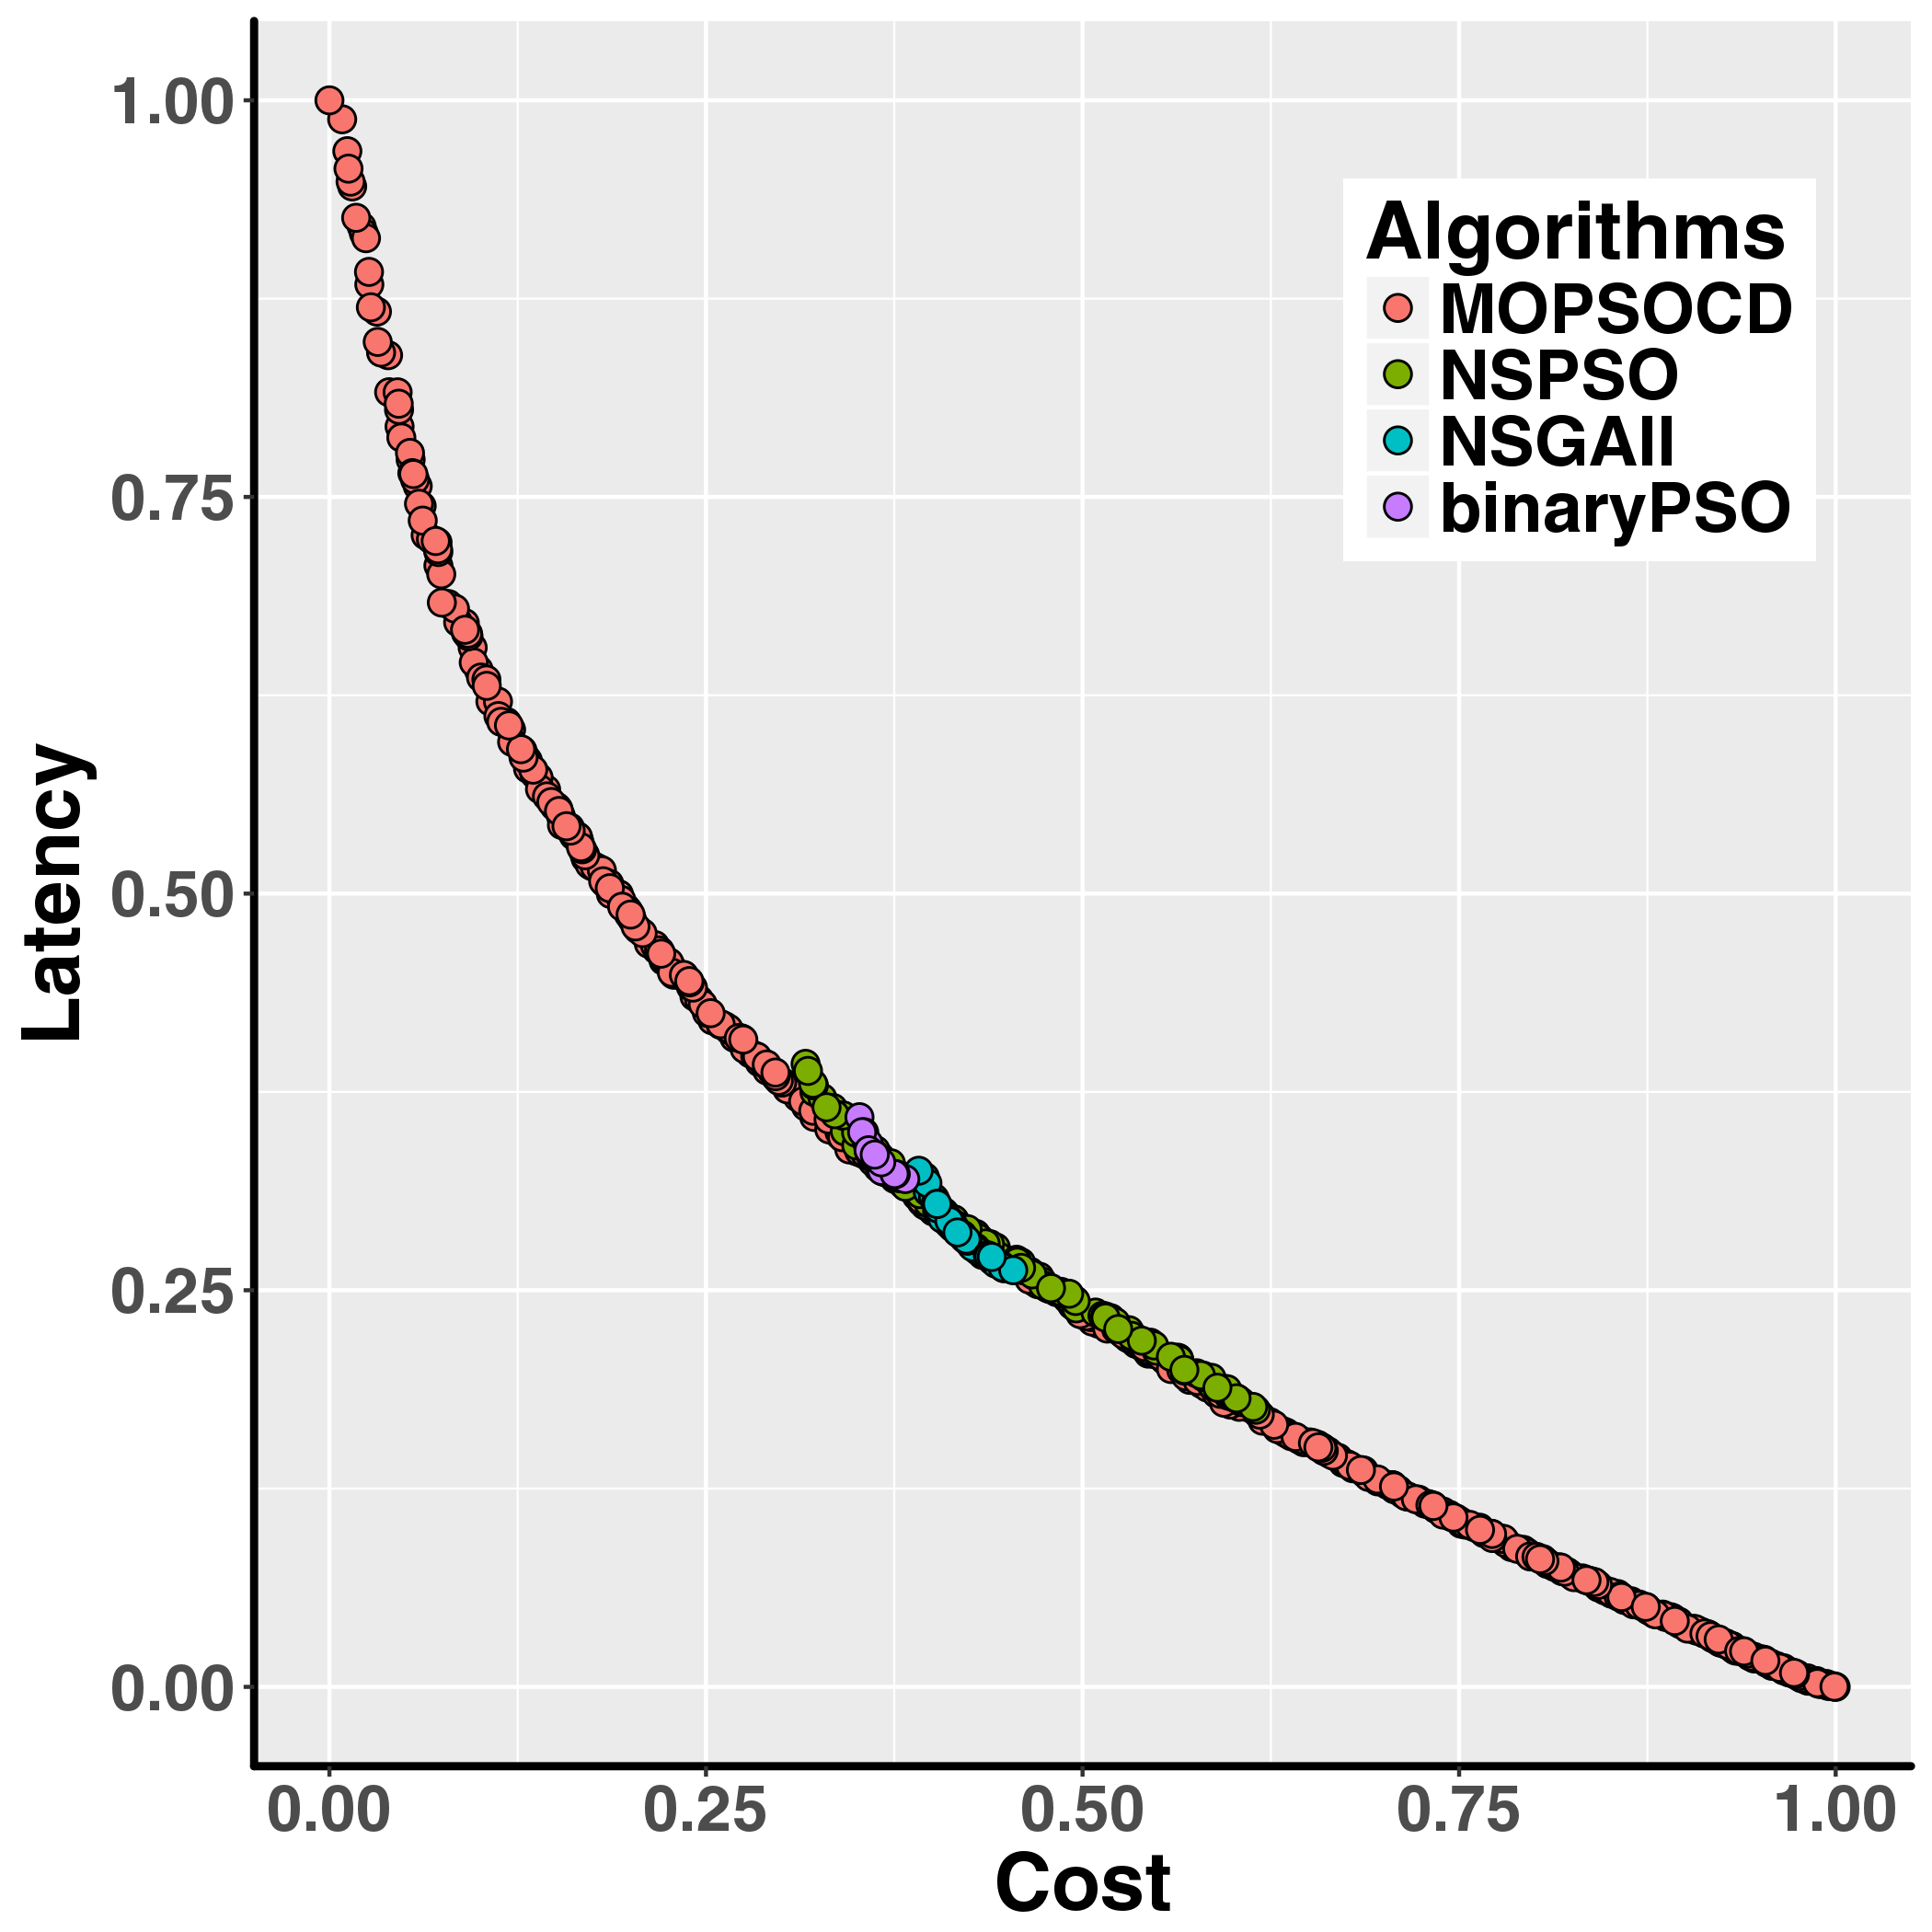
\includegraphics[width=\textwidth]{pics/total13.png}
    \caption{instance 13}
   \end{subfigure}
      \begin{subfigure}{0.21\linewidth}
       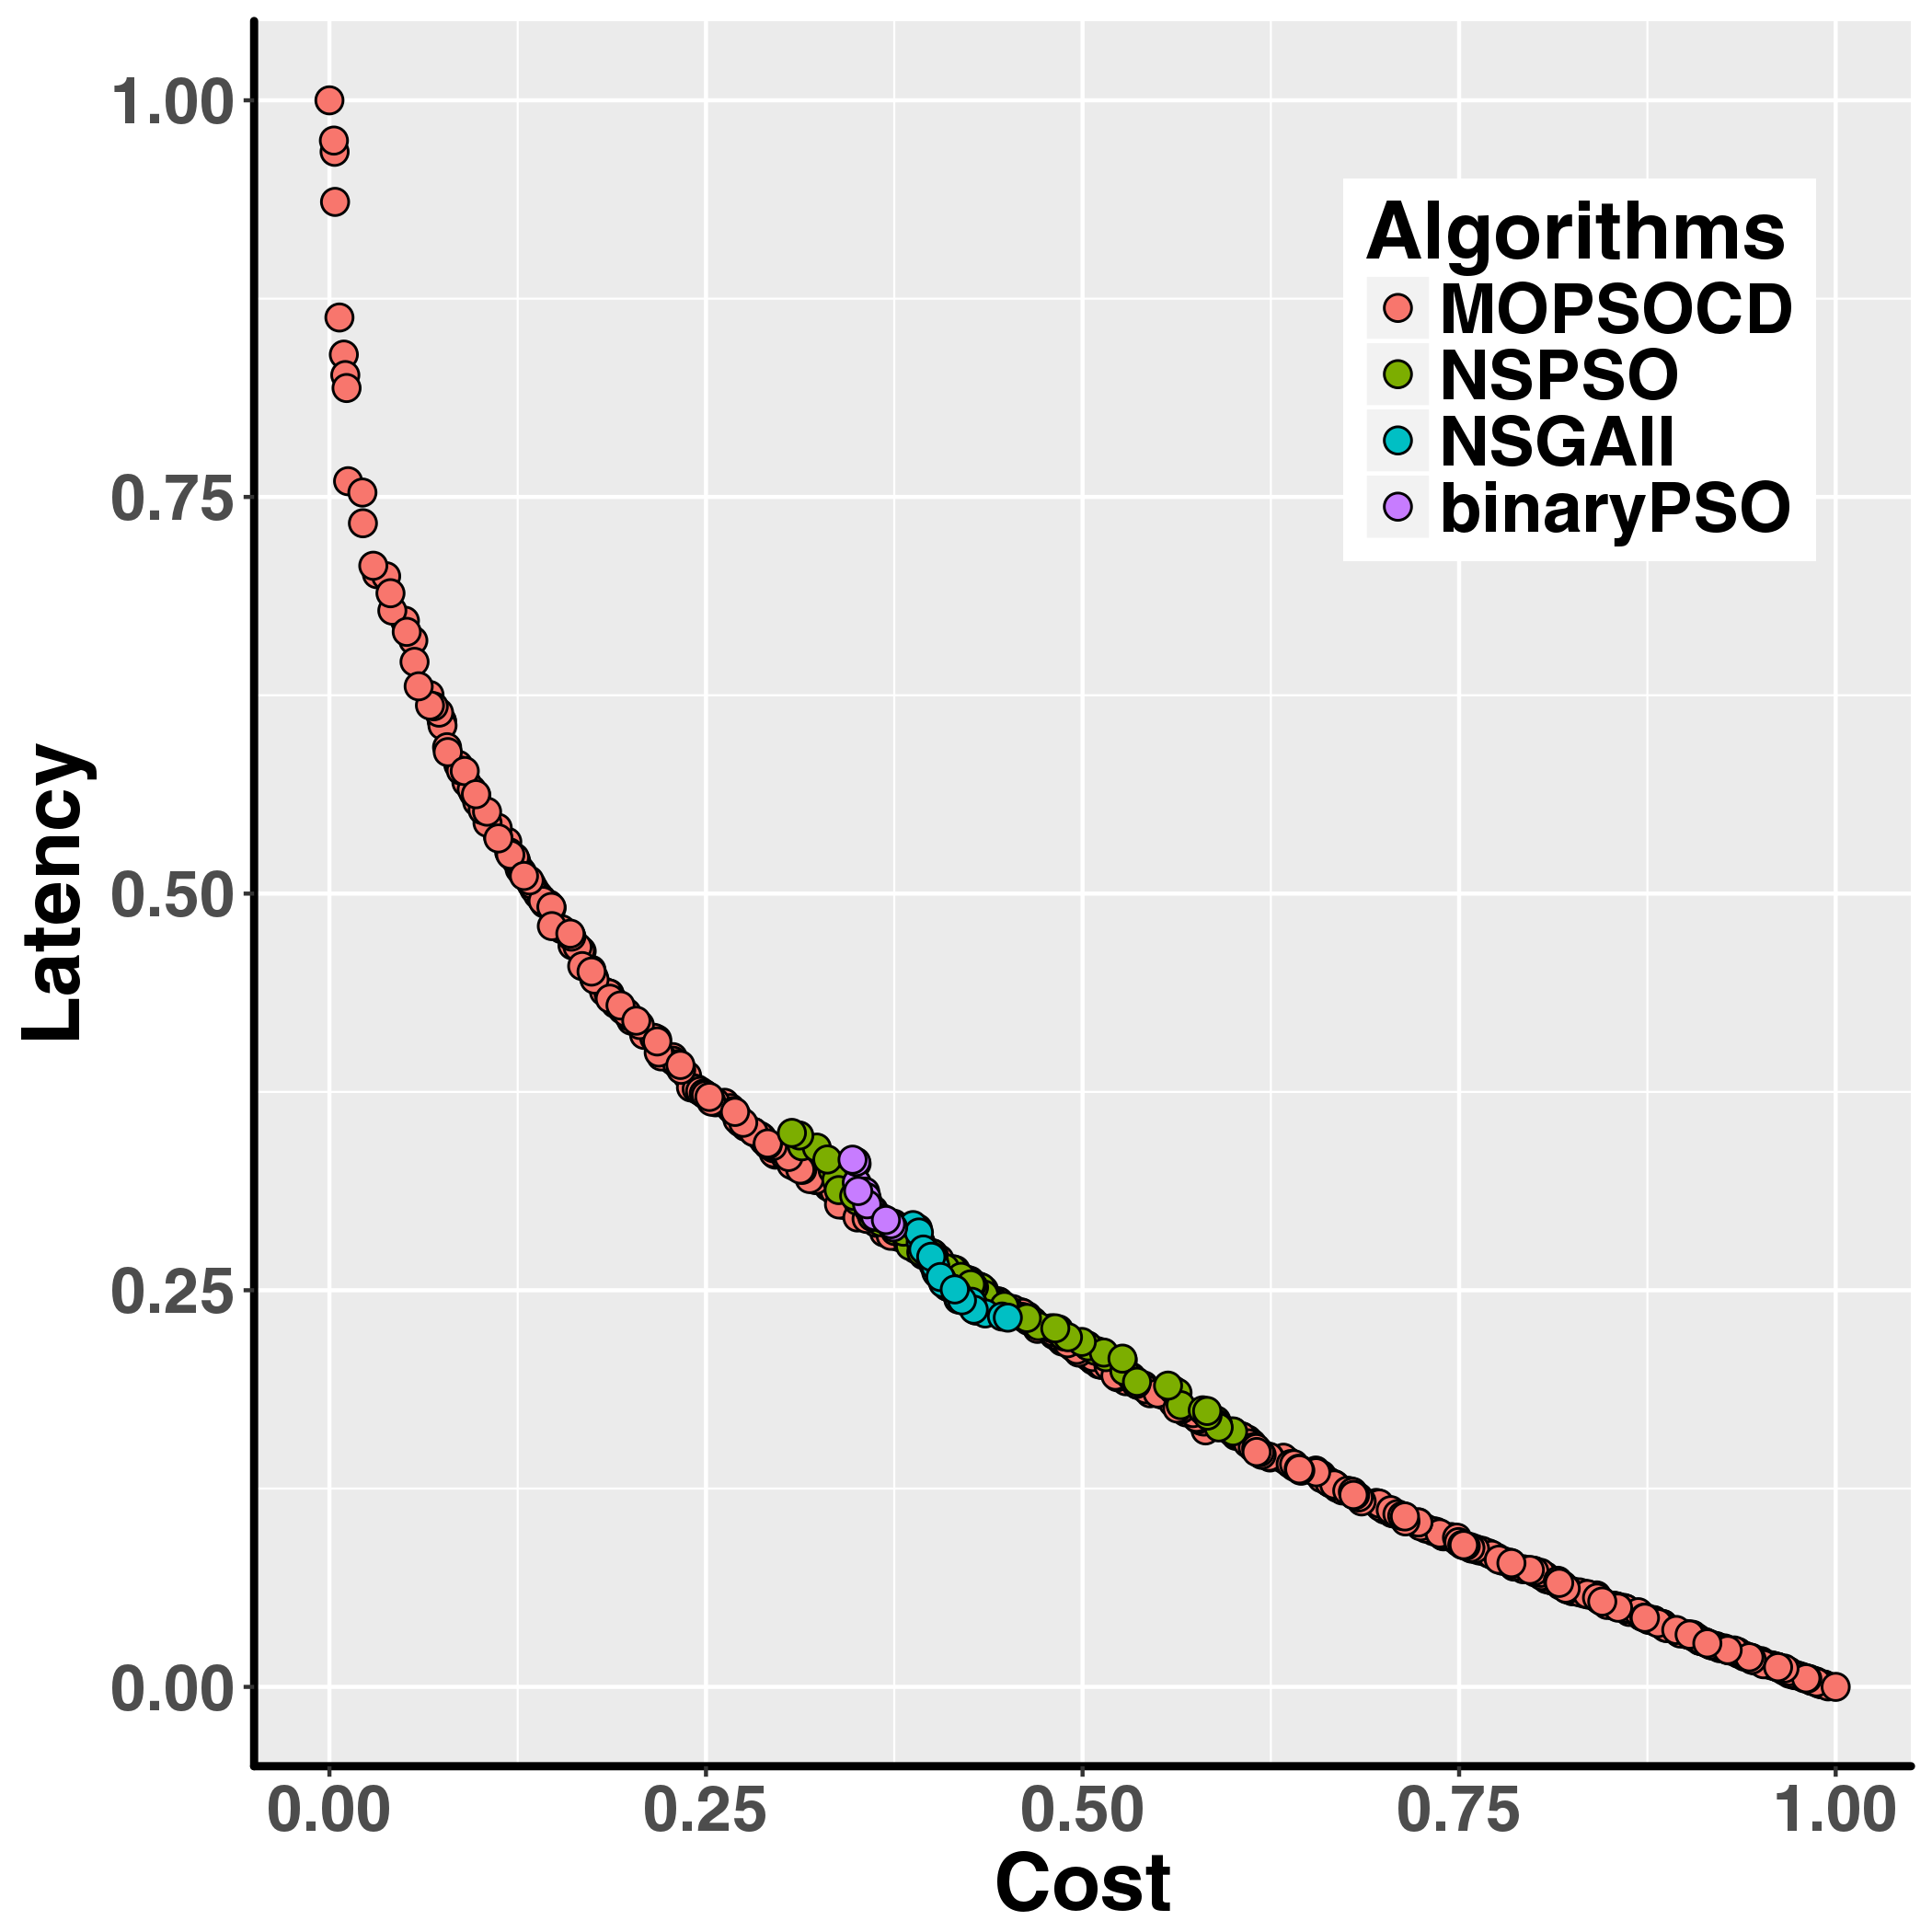
\includegraphics[width=\textwidth]{pics/total14.png}
    \caption{instance 14}
   \end{subfigure}
   \caption{MOPSOCD, BNSPSO, NSGA-II, and BPSO Experiments: The non-dominated solutions
among the sets obtained by 40 independent runs of different algorithms}

   \label{fig:total}
\end{figure*}

% \begin{table}[ht]
% \centering
% \caption{My caption}
% \label{my-label}
% \begin{tabular}{@{}ccc@{}}
% \toprule
% \multicolumn{1}{l}{Solution} & \multicolumn{1}{l}{Cost} & \multicolumn{1}{l}{Response time} \\ \midrule
% A                            & 1000                     & 3.5s                              \\
% B                            & 500                      & 15s                               \\
% C                            & 800                      & 10s                               \\
% D                            & 900                      & 12s                               \\ \bottomrule
% \end{tabular}
% \end{table}

% \begin{figure}[ht]
% 	\centering
% 	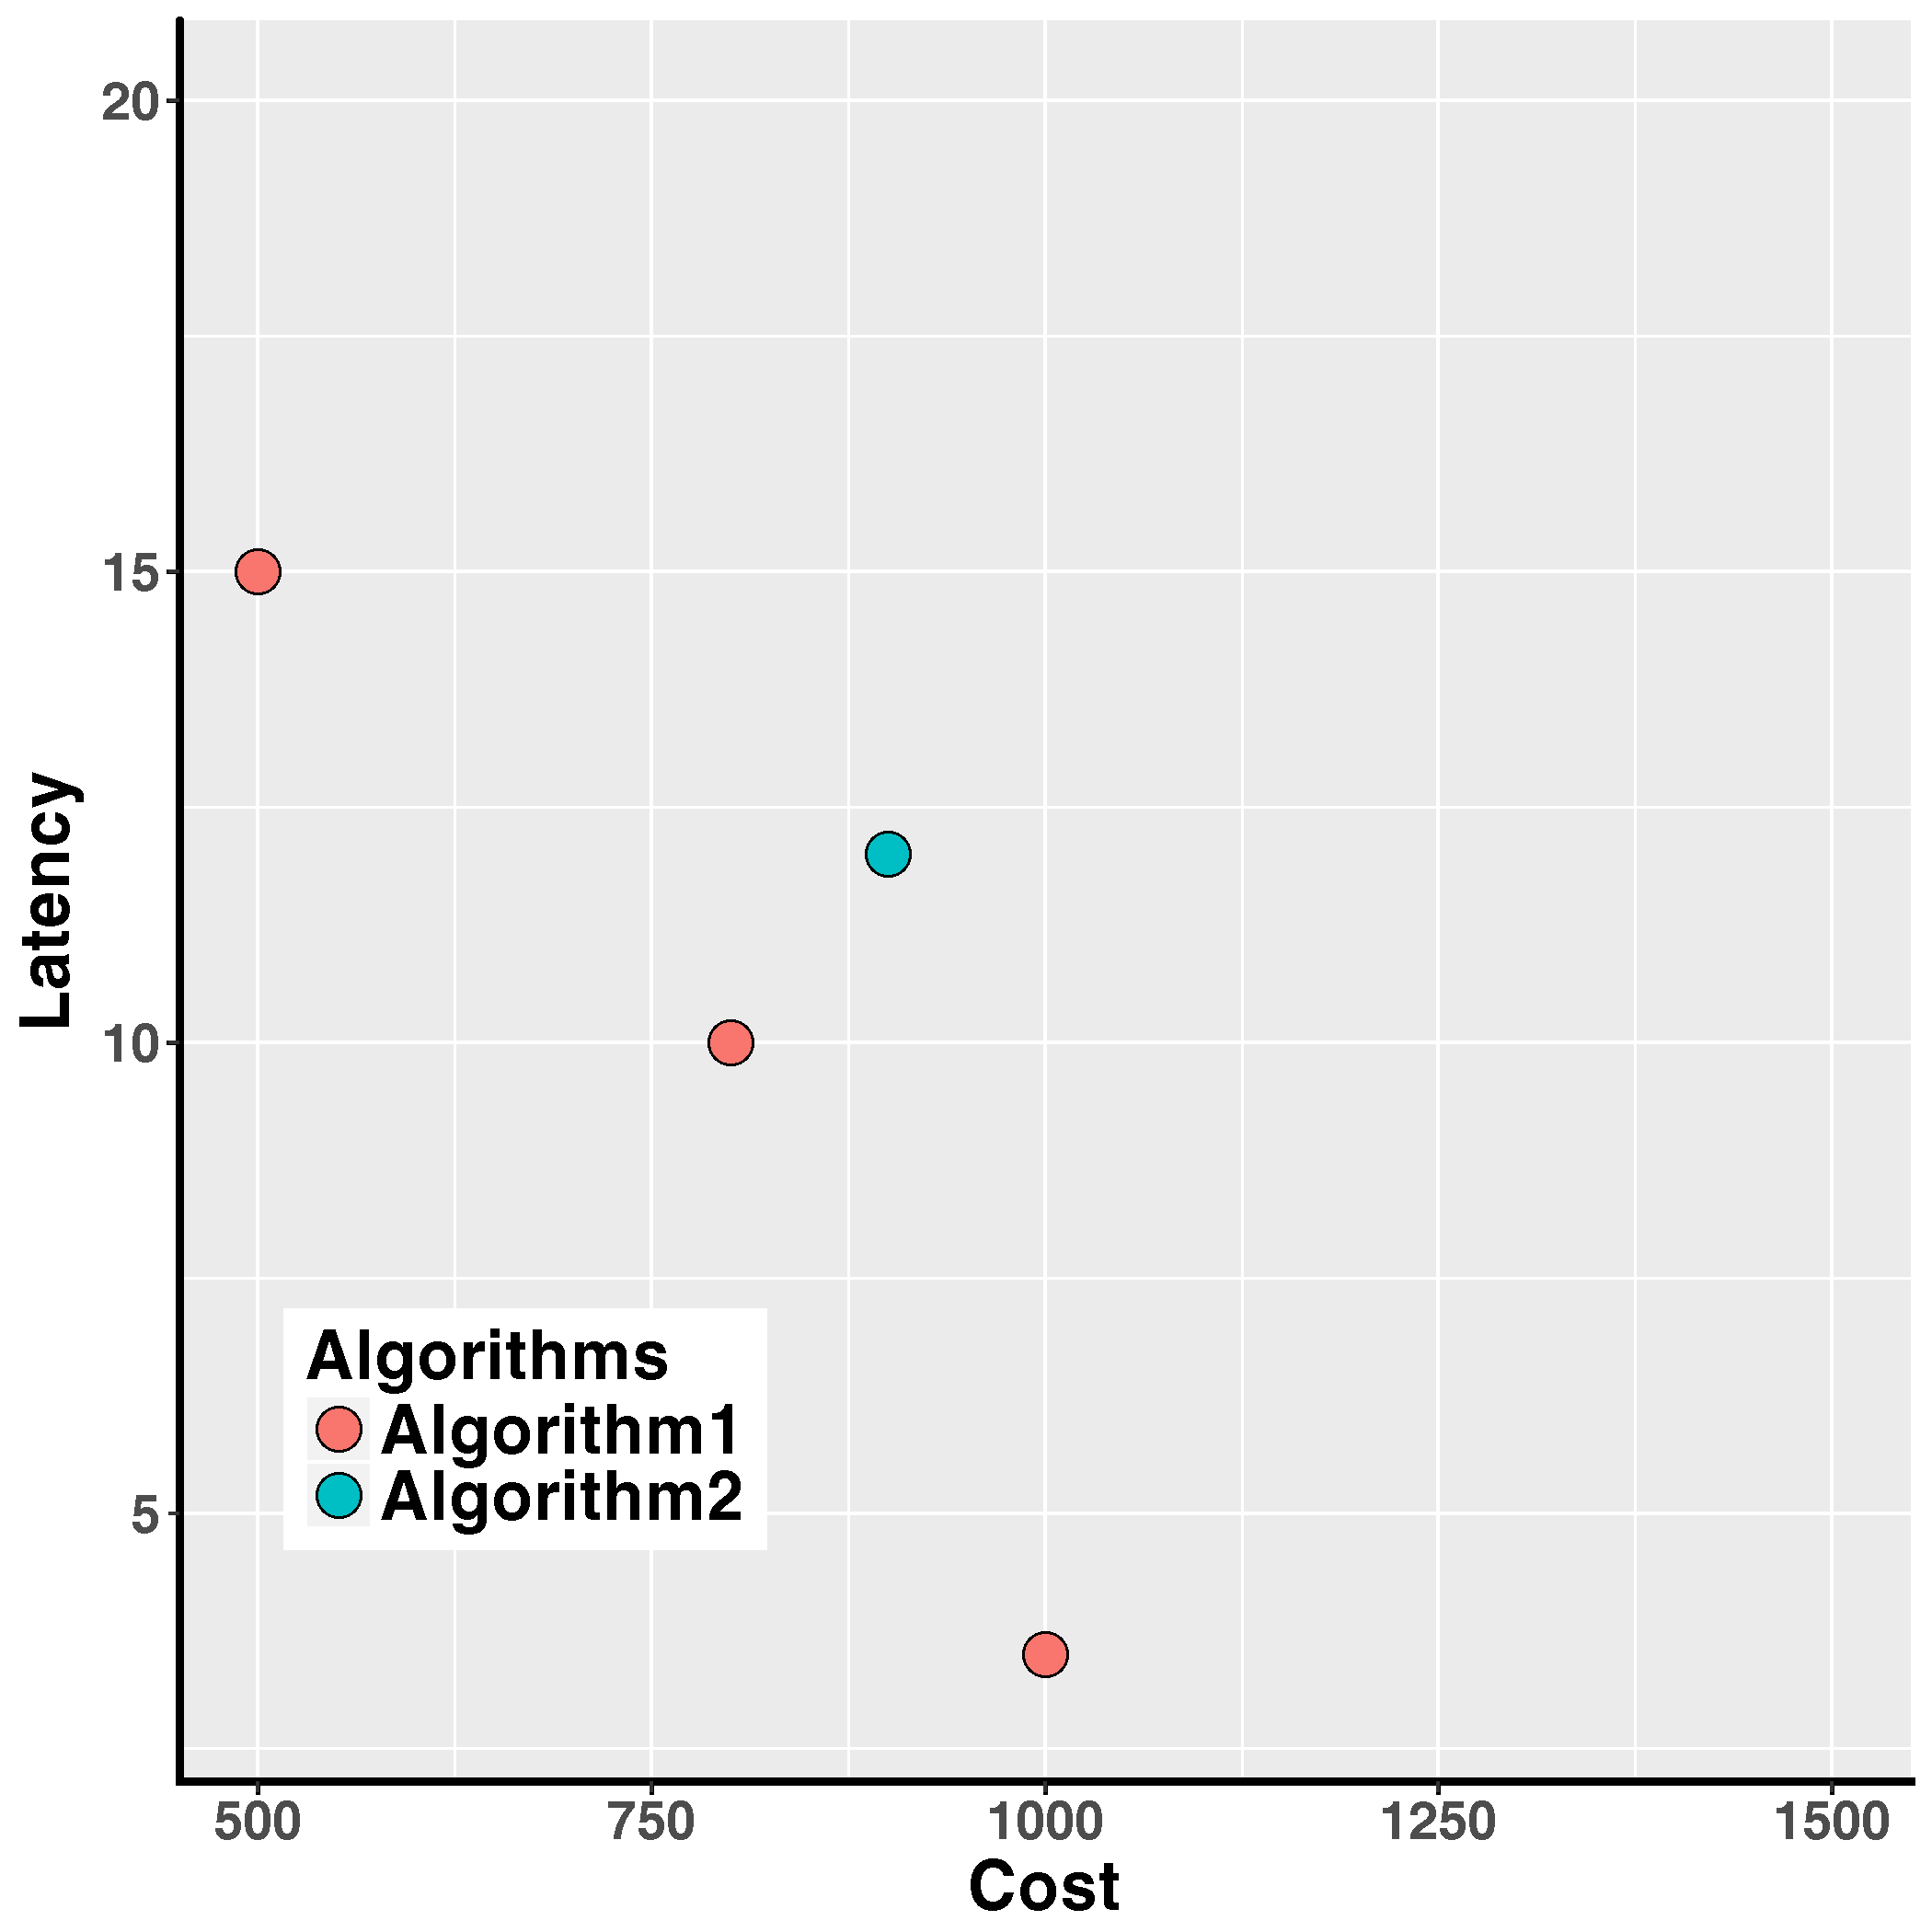
\includegraphics[width=0.35\textwidth]{pics/example.png}
% 	\caption{Comparison between multi-objective and single-objective algorithms}
% 	\label{fig:example}
% \end{figure}

In summary, from the experimental evaluation comparing the proposed algorithm with previous approaches, we observe that on most test instances, BMOPSOCD can achieve much better results than BNSPSO, NSGA-II, and BPSO in both convergence and diversity. The performance of MOPSOCD with dynamic rounding function is not much affected by the number of variables. This is a significant advantage of BMOPSOCD over the other three approaches.

% \subsection{BMOPSOCD versus Greedy approaches}
% To evaluate the impact of our proposed algorithm to the users, we design two greedy approaches which represent general solutions for industrial service providers. Each greedy algorithm aims at 
% minimizing overall cost and latency respectively. 
\vspace{-3 mm}
\section{Related Work}\label{sec:related}



Location-allocation problems with immobile servers such as hospitals, stores and disposal centers have arisen for a long time \cite{Vidyarthi201420}. The main characteristic of this problem is that customers need to travel to servers for services in contrast with mobile servers traveling to customers in response to requests. Similar to WSLAP, response time represents customer traveling time and network latency has a strong impact on response time between customers' locations and web services' locations. 



Most previous researchers treated WSLAP as a single objective problem and proposed many simple greedy-based heuristic algorithms, such as ADD, DROP and Alternate Location Allocation (ALA) \cite{Sun}.  As an improvement, Sun et al. \cite{Sun} proposed a DAL method which combines DROP, ALA and Linear Programming relaxations of Integer Transportation problems. Aboolian et al \cite{Aboolian} introduced a location-allocation model for a web service provider in duopoly competitive market. They solved the problem with Integer Linear Programming (ILP) technique. Goiri et al. \cite{5961695} proposed a novel combination of linear programming and simulated annealing approach for allocation of data centers for Internet services. 
Yuk and Lin \cite{lin2014solving} considered not only facility location and demand allocation, but also resource capacity allocation (number of service replicas). They formulated the problem as a stochastic mixed integer program and proposed a simulation-based hybrid heuristic to solve the dynamic problem under different response time service level.
In contrast, in our previous studies \cite{Tan2016a,Tan2016}, we proposed a multi-objective algorithm with linear aggregation using PSO and a multi-objective algorithm with Pareto front using NSGA-II. Both results show that 
multi-objective model suits the problem well. The solutions contain a set of equally good allocations trade off between cost and service response time. Hence, the service providers can select the most suitable allocation according to their preferences. 

For example, a multi-objective algorithm gives a solution set contains many solutions, among them, solution A is \{cost: 1000, response time: 3.5s\}, solution B is \{cost: 500, response time: 15s\}, and solution C is \{cost:800, response time: 10s\}. A single-objective algorithm gives a solution D: \{cost: 900, 12s\}. In this case, solution C better than solution D in both objectives (cost: 800 $<$ 900, response: 10s $<$ 12s).

Meanwhile, if a service provider would like to provide the best service quality to customers without caring too much of the budget, then solution A is the most suitable choice. Conversely, a service provider with tight budget may choose solution C. 
Service providers can balance their profit with our multi-objective model.
% Both approaches can provide good results with reasonable time. Nevertheless, for linear aggregation approach, the solutions are not diverse enough for service providers. 

We can see from the previous example, a service provider can select a suitable solution if the solution set is diverse enough - a provider may have precise requirement (e.g. cost $<$ 525, response $<$ 14.5s). The new approach can provide a much more diverse solution set compared with our
previous approaches including BPSO, BNSPSO, and NSGA-II (see Figure. \ref{fig:total}). This is a major contribution.

In addition, the major limitation of Integer Linear Programming is that the computational time increases rapidly when the size of the problem increases. Torrent-Fontbona et al. \cite{TorrentFontbona20134593} proposed a method that first uses clustering technique to reduce the complexity and then applied heuristic methods to solve the problem. It reduces the computation time as well as the quality of the solutions. However, our proposed algorithms can deal with large
test instance with hundreds of services and more. Our BMOPSOCD shows none-degradation with the number of variables increasing.


% In order to solve the scalability problem, Huang et al. \cite{EnhancedGenetic} proposed an enhanced genetic algorithm on WSLAP. They modeled the dependencies between services as an invocation probability and optimize the total cost of deployed services as the single objective. The result showed that the proposed algorithm can provide near optimum solutions within reasonable amount of time. Nevertheless, as WSLAP is inherently a multi-objective problem, single-objective methods cannot capture the tradeoff between two conflicting objectives.
% We further extended Huang's formulation into a multi-objective problem with minimization of cost and latency as objectives. 


% Pasandideh et al. \cite{pasandideh2012genetic} studied the facility allocation problem, which takes stochastic customer demands the input. They treated it as a multi-objective problem with minimizations of customer waiting time and average facility idle time percentage as objectives. A GA-based approach was proposed to solve this problem and it showed that the proposed GA could largely reduce the computation time while obtaining near optimum solutions.


With the emergence of cloud computing, virtual machine allocation problem is becoming important for service providers and cloud providers. Instead of allocating web services to physical servers, web services are first allocated to virtual machines(VMs) and then VMs are allocated to physical machines. The problem of VM allocation is 
similar to WSLAP with multiple objectives and binary VM allocation. Kessaci et al. \cite{6557869} proposed an MOGA-CB for minimizing the cost of VMs and response time when considering web service composition as a workflow. Phan et al. \cite{Phan8} proposed a framework called Green Monster, to dynamically move web services across Internet data centers for reducing their carbon footprint while maintaining their performance. Greenmonster applied a modified version of NSGA-II algorithm \cite{nsgaii} with an additional local search process. Our BMOPSOCD can solve VM allocation problem with minor modification of objective and constraint functions. Therefore, 
BMOPSOCD is useful for Cloud providers.


\vspace{-3 mm}
\section{Conclusion and Future Work} \label{sec:conclusion}

This paper proposed a BMOPSOCD to solve the WSLAP with the aim of producing a set of high-quality solutions that covers most of the Pareto front when dealing with large test instances. For that, we proposed a binary version of multi-objective PSO with crowding distance to solve the WSLAP. We employed a rounding function mechanism which not only makes a continuous algorithm compatible with binary problems but also significantly improves the quality of solutions. Three types of rounding functions were developed. From the experiments, we observed that the solutions obtained by BMOPSOCD with dynamic rounding functions have a great diversity that almost covers the whole Pareto front. Meanwhile, BMOPSOCD could produce good solutions regardless of the increasing problem size. For service providers who use this algorithm to design the allocation of their services, there are several advantages. First of all, BMOPSOCD can provide near optimum solutions in comparison with solutions from greedy-based heuristic algorithms. Secondly, it provides a wider range of non-dominated solutions compares with single-objective algorithms. In addition, near-optimal solutions are given within a feasible amount of time.

%The major contribution is that we provide a rounding function and an adaptive threshold technique to make a continuous algorithm compatible with a binary problem. These techniques can also be applied in other continuous algorithms. We have shown that BMOPSOCD can produce solutions with a good diversity that covers most of the Pareto front.

There are a few directions that we can work on in the future. Firstly, our model can be further improved by considering service composition. For now, the problem model considers each service as an atomic service. With the increasing usages of composite services composed with atomic services distributed over the Internet \cite{6900416,Tan2017}, we need to consider service composition workflow while solving WSLAP.   Service composition workflows have a significant impact on the allocation of atomic services because the data flow between services could not be neglected. Therefore, the location of each atomic service is highly related to the previous and the next service in a workflow.

Secondly, more potential objectives need to be considered, for example, maximizing availability of services. To avoid single point failure, web service providers often deploy many copies of service in different candidate locations to ensure the availability. 

In addition, service deployment in Cloud becomes a hot topic between service computing and cloud computing. Cloud computing provides an elastic resource management for services so that it removes the burden of managing hardwares for service providers. However, new issues such as dynamic virtual machine placement for service composition, elastic resource management for services have emerged \cite{7969618}. Difficult (often NP-hard) and dynamic nature make it extremely challenging.
% Green economy could also be considered. As the issue of global warming becomes a global challenge, deploying a service to a location that is closed to a power plant has been proposed in the literature . In addition, future work can consider multiple constraints such as the overall cost constraints and bandwidth constraints.

%\ifCLASSOPTIONcaptionsoff
 %\newpage
%\fi



\section*{Acknowledgment}
This work is supported in part by the New Zealand Marsden Fund with the contract numbers (VUW1510 and VUW1614), administrated by the Royal Society of New Zealand.


\bibliographystyle{IEEEtran}

\bibliography{sample}
\small
\begin{IEEEbiography}[{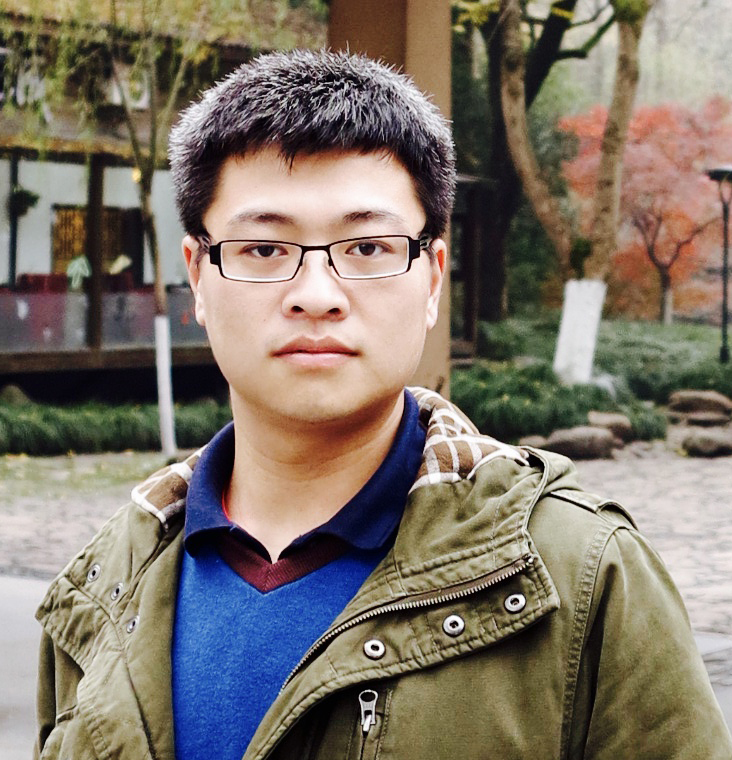
\includegraphics[width=1in,height=1.25in,clip,keepaspectratio]{photo/BoxiongTan}}]{Boxiong Tan}
is a Ph.D. student at the School of Engineering and Computer Science, Victoria University of
Wellington, Wellington, New Zealand. He received B.E degree from Guangzhou University and MCS degree from Victoria University of
Wellington in 2011 and 2016 respectively.
\end{IEEEbiography}
\vspace{-9.5 mm}
\begin{IEEEbiography}[{
\includegraphics[width=1in,height=1.25in,clip,keepaspectratio]{photo/HuiMa}}]{Hui Ma}
received her B.E. degree from Tongji University and her B.S. (Hons.), M.S. and Ph.D. degrees from Massay University. She is currently a Senior Lecturer in Software Engineering at Victoria University of Wellington. Her research interests include service computing, conceptual modelling, database systems, resource allocation in clouds, and evolutionary computation in combinatorial optimization.

Hui has more than 80 publications, including leading journals and conferences in databases, service computing, evolutionary computation, and conceptual modelling, such as Journal of Heuristics, Data \& Knowledge Engineering (DKE), the International Conference on Conceptual Modeling (ER), and Genetic and Evolutionary Computation Conference (GECCO). She has served as a PC member for about 60 international conferences, including seven times as a PC chair for conferences such as ER, DEXA, and APCCM. She is serving as a member of the ER steering committee and the IEEE CIS Emergent Technology technical committee.
\end{IEEEbiography}
\vspace{-9.5 mm}
\begin{IEEEbiography}[{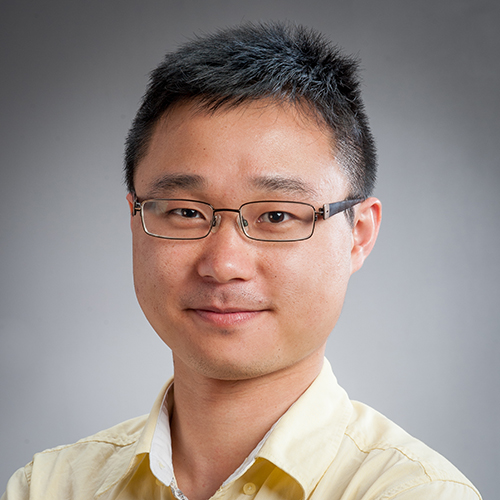
\includegraphics[width=1in,height=1.25in,clip,keepaspectratio]{photo/YiMei}}]{Yi Mei} (M’09)
is a lecturer at the School of Engineering and Computer Science, Victoria University of Wellington, Wellington, New Zealand. He received his BSc and PhD degrees from University of Science and Technology of China in 2005 and 2010, respectively. His research interests include evolutionary computation in scheduling, routing and combinatorial optimization, as well as evolutionary machine learning, hyper-heuristics, genetic programming, feature selection and dimensional reduction.

Yi has more than 60 fully referred publications, including the top journals in EC and Operations Research (OR) such as IEEE TEVC, IEEE Transactions on Cybernetics, European Journal of Operational Research, ACM Transactions on Mathematical Software, and top EC conferences (GECCO). As the sole investigator, he won the 2nd prize of the Competition at IEEE WCCI 2014: Optimization of Problems with Multiple Interdependent Components. He serves as a Vice-Chair of the IEEE CIS Emergent Technologies Technical Committee, and a member of three IEEE CIS Task Forces and two IEEE CIS Technical Committees. He is an Editorial Board Member of International Journal of Bio-Inspired Computation, and a guest editor of a special issue of the Genetic Programming Evolvable Machine journal. He has organised a number of special sessions in international conferences such as IEEE CEC. He serves as a reviewer of over 25 international journals including the top journals in EC and OR.
% He has organized a number of special sessions in international conferences such as IEEE CEC. He serves as a reviewer of over 25 international journals including the top journals in EC and OR.
% As  the  sole
% investigator, he won the 2nd prize of the Competition at IEEE WCCI 2014: Optimisation  of  Problems  with  Multiple  Interdependent  Components.  He
% received  the  2010  Chinese  Academy  of  Sciences  Dean's  Award  (top 200 postgraduates all over China) and the 2009 IEEE Computational Intelligence
% Society (CIS) Postgraduate Summer Research Grant (three to four recipients all over the world). He is serving as the committee member of IEEE ECTC
% Task  Force  on  Evolutionary  Scheduling  and  Combinatorial  Optimisation, IEEE  CIS  Task  Force  on  EC  for  Feature  Selection  and  Construction  and
% IEEE  CIS  Task  Force  on  Large  Scale  Global  Optimisation. 
\end{IEEEbiography}
\vspace{-9.5 mm}
\begin{IEEEbiography}[{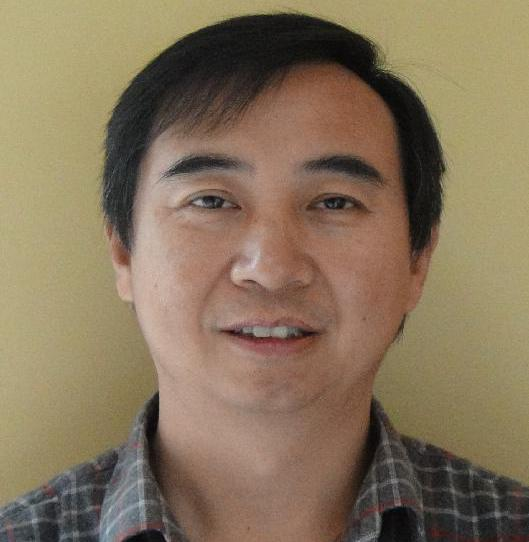
\includegraphics[width=1in,height=1.25in,clip,keepaspectratio]{photo/MengjieZhang}}]{Mengjie Zhang} (M’04-SM’10)
received the B.E. and M.E. degrees from Artificial Intelligence Research Center, Agricultural University of Hebei, Hebei, China, and the Ph.D. degree in computer science from RMIT University, Melbourne, Australia, in 1989, 1992, and 2000, respectively.

Since 2000, he has been with the Victoria University of Wellington, Wellington, New Zealand, where he is currently Professor of Computer Science, the Head of the Evolutionary Computation Research Group, and Associate Dean (Research and Innovation) in the Faculty of Engineering. His current research interests include artificial intelligence, machine learning and big data, particularly in evolutionary computation and learning, genetic programming, image analysis, feature selection and big dimensionality reduction, evolutionary scheduling and combinatorial optimization, and evolutionary deep learning and transfer learning. He has published over 450 research papers in refereed international journals and conferences.

Mengjie is a Fellow of Royal Society of New Zealand, and has been serving as an Associated Editor for over ten international journals (including IEEE Transactions on Evolutionary Computation, IEEE Transactions on Cybernetics, Evolutionary Computation Journal, and IEEE Transactions on Emergent Topics in CI) and as a Reviewer of over 30 international journals. He has been serving as a Steering Committee Member and a Program Committee Member for over 100 international conferences. He has supervised over 50  postgraduate research students. He is the Chair of the IEEE CIS Intelligent Systems and Applications Technical Committee, an Immediate Past Chair of the IEEE CIS Evolutionary Computation Technical Committee, a Vice-Chair of the IEEE CIS Task Force on Evolutionary Computer Vision and Image Processing, a Vice-Chair of the IEEE CIS  Task Force on Evolutionary Computation for Feature Selection and Construction, a member of IEEE CIS Task Force of Hyper-heuristics, and the Founding Chair for IEEE Computational Intelligence Chapter in New Zealand.
\end{IEEEbiography}


\end{document}






% The rounding process can be done in fitness function so that there is no need to modify the PSO.

% We introduced a \emph{service location-allocation probability matrix}, $A' = [a'_{sj}]$ represents the probability of a
% service $s_{i}$ allocate to a candidate location $j_{i}$.
% $a'_{sj}$ is a real-valued, $a'_{sj} \in (0, 1)$ indicate the probability of a service is \textbf{NOT}
% allocate to a candidate location.
%
% We use the service location-allocation probability matrix $A'$ = $[a'_{sj}]$ as a particle.
% During the PSO process, the particle needs to be transfered to binary representation in order to compatible with
% the modeling. In order to transfer $A' \rightarrow A$, we introduced a transformation
% function.
%







